%-------------------------------------------------------------------------------
% PACKAGES AND OTHER DOCUMENT CONFIGURATIONS
%-------------------------------------------------------------------------------

\documentclass[11pt,fleqn]{book} % Default font size and left-justified equations
\usepackage[top=3cm,bottom=3cm,left=3.2cm,right=3.2cm,headsep=10pt,a4paper]{geometry} % Page margins
\usepackage{kotex}
\usepackage[unicode]{hyperref}
\usepackage{xcolor} % Required for specifying colors by name
\definecolor{ocre}{RGB}{243,102,25} % Define the orange color used for highlighting throughout the book

\usepackage{avant} % Use the Avantgarde font for headings
%\usepackage{times} % Use the Times font for headings
\usepackage{mathptmx} % Use the Adobe Times Roman as the default text font together with math symbols from the Symbol, Chancery and Computer Modern fonts
\usepackage{microtype} % Slightly tweak font spacing for aesthetics
\DisableLigatures{encoding = *, family = *} % Note that this will also disable ligatures such as "--" to "–", "---" to "—", etc.

% Bibliography
\usepackage[style=alphabetic,sorting=nyt,sortcites=true,autopunct=true,babel=hyphen,hyperref=true,abbreviate=false,backref=true,backend=biber]{biblatex}
\addbibresource{bibliography.bib} % BibTeX bibliography file
\defbibheading{bibempty}{}

% Index
\usepackage{calc} % For simpler calculation - used for spacing the index letter headings correctly
\usepackage{makeidx} % Required to make an index
\makeindex % Tells LaTeX to create the files required for indexing
\usepackage{tikz}
\newcommand*\circled[1]{\tikz[baseline=(char.base)]{
            \node[shape=circle,draw,inner sep=1pt] (char) {#1};}}
\newcounter{num}
% \newcounter{num}\setcounter{num}{0}
% \stepcounter{num}\circled{\thenum}
% \usepackage[english]{babel}
\renewcommand{\figurename}{그림}

%-------------------------------------------------------------------------------

% -*- root: main.tex -*-
%----------------------------------------------------------------------------------------
%	VARIOUS REQUIRED PACKAGES
%----------------------------------------------------------------------------------------

\usepackage{titlesec} % Allows customization of titles

\usepackage{graphicx} % Required for including pictures
\graphicspath{{pictures/}} % Specifies the directory where pictures are stored

\usepackage{lipsum} % Inserts dummy text

\usepackage{tikz} % Required for drawing custom shapes

\usepackage[english]{babel} % English language/hyphenation

\usepackage{enumitem} % Customize lists
\setlist{nolistsep} % Reduce spacing between bullet points and numbered lists

\usepackage{booktabs} % Required for nicer horizontal rules in tables

\usepackage{eso-pic} % Required for specifying an image background in the title page

%----------------------------------------------------------------------------------------
%	MAIN TABLE OF CONTENTS
%----------------------------------------------------------------------------------------

\usepackage{titletoc} % Required for manipulating the table of contents

\contentsmargin{0cm} % Removes the default margin
% Chapter text styling
\titlecontents{chapter}[1.25cm] % Indentation
{\addvspace{15pt}\large\sffamily\bfseries} % Spacing and font options for chapters
{\color{ocre!60}\contentslabel[\Large\thecontentslabel]{1.25cm}\color{ocre}} % Chapter number
{}  
{\color{ocre!60}\normalsize\sffamily\bfseries\;\titlerule*[.5pc]{.}\;\thecontentspage} % Page number
% Section text styling
\titlecontents{section}[1.25cm] % Indentation
{\addvspace{5pt}\sffamily\bfseries} % Spacing and font options for sections
{\contentslabel[\thecontentslabel]{1.25cm}} % Section number
{}
{\sffamily\hfill\color{black}\thecontentspage} % Page number
[]
% Subsection text styling
\titlecontents{subsection}[1.25cm] % Indentation
{\addvspace{1pt}\sffamily\small} % Spacing and font options for subsections
{\contentslabel[\thecontentslabel]{1.25cm}} % Subsection number
{}
{\sffamily\;\titlerule*[.5pc]{.}\;\thecontentspage} % Page number
[] 

%----------------------------------------------------------------------------------------
%	MINI TABLE OF CONTENTS IN CHAPTER HEADS
%----------------------------------------------------------------------------------------

% Section text styling
\titlecontents{lsection}[0em] % Indendating
{\footnotesize\sffamily} % Font settings
{}
{}
{}

% Subsection text styling
\titlecontents{lsubsection}[.5em] % Indentation
{\normalfont\footnotesize\sffamily} % Font settings
{}
{}
{}
 
%----------------------------------------------------------------------------------------
%	PAGE HEADERS
%----------------------------------------------------------------------------------------

\usepackage{fancyhdr} % Required for header and footer configuration

\pagestyle{fancy}
\renewcommand{\chaptermark}[1]{\markboth{\sffamily\normalsize\bfseries\chaptername\ \thechapter.\ #1}{}} % Chapter text font settings
\renewcommand{\sectionmark}[1]{\markright{\sffamily\normalsize\thesection\hspace{5pt}#1}{}} % Section text font settings
\fancyhf{} \fancyhead[LE,RO]{\sffamily\normalsize\thepage} % Font setting for the page number in the header
\fancyhead[LO]{\rightmark} % Print the nearest section name on the left side of odd pages
\fancyhead[RE]{\leftmark} % Print the current chapter name on the right side of even pages
\renewcommand{\headrulewidth}{0.5pt} % Width of the rule under the header
\addtolength{\headheight}{2.5pt} % Increase the spacing around the header slightly
\renewcommand{\footrulewidth}{0pt} % Removes the rule in the footer
\fancypagestyle{plain}{\fancyhead{}\renewcommand{\headrulewidth}{0pt}} % Style for when a plain pagestyle is specified

% Removes the header from odd empty pages at the end of chapters
\makeatletter
\renewcommand{\cleardoublepage}{
\clearpage\ifodd\c@page\else
\hbox{}
\vspace*{\fill}
\thispagestyle{empty}
\newpage
\fi}

%----------------------------------------------------------------------------------------
%	THEOREM STYLES
%----------------------------------------------------------------------------------------

\usepackage{amsmath,amsfonts,amssymb,amsthm} % For math equations, theorems, symbols, etc

\newcommand{\intoo}[2]{\mathopen{]}#1\,;#2\mathclose{[}}
\newcommand{\ud}{\mathop{\mathrm{{}d}}\mathopen{}}
\newcommand{\intff}[2]{\mathopen{[}#1\,;#2\mathclose{]}}
\newtheorem{notation}{Notation}[chapter]

%%%%%%%%%%%%%%%%%%%%%%%%%%%%%%%%%%%%%%%%%%%%%%%%%%%%%%%%%%%%%%%%%%%%%%%%%%%
%%%%%%%%%%%%%%%%%%%% dedicated to boxed/framed environements %%%%%%%%%%%%%%
%%%%%%%%%%%%%%%%%%%%%%%%%%%%%%%%%%%%%%%%%%%%%%%%%%%%%%%%%%%%%%%%%%%%%%%%%%%
\newtheoremstyle{ocrenumbox}% % Theorem style name
{0pt}% Space above
{0pt}% Space below
{\normalfont}% % Body font
{}% Indent amount
{\small\bf\sffamily\color{ocre}}% % Theorem head font
{\;}% Punctuation after theorem head
{0.25em}% Space after theorem head
{\small\sffamily\color{ocre}\thmname{#1}\nobreakspace\thmnumber{\@ifnotempty{#1}{}\@upn{#2}}% Theorem text (e.g. Theorem 2.1)
\thmnote{\nobreakspace\the\thm@notefont\sffamily\bfseries\color{black}---\nobreakspace#3.}} % Optional theorem note
\renewcommand{\qedsymbol}{$\blacksquare$}% Optional qed square

\newtheoremstyle{blacknumex}% Theorem style name
{5pt}% Space above
{5pt}% Space below
{\normalfont}% Body font
{} % Indent amount
{\small\bf\sffamily}% Theorem head font
{\;}% Punctuation after theorem head
{0.25em}% Space after theorem head
{\small\sffamily{\tiny\ensuremath{\blacksquare}}\nobreakspace\thmname{#1}\nobreakspace\thmnumber{\@ifnotempty{#1}{}\@upn{#2}}% Theorem text (e.g. Theorem 2.1)
\thmnote{\nobreakspace\the\thm@notefont\sffamily\bfseries---\nobreakspace#3.}}% Optional theorem note

\newtheoremstyle{blacknumbox} % Theorem style name
{0pt}% Space above
{0pt}% Space below
{\normalfont}% Body font
{}% Indent amount
{\small\bf\sffamily}% Theorem head font
{\;}% Punctuation after theorem head
{0.25em}% Space after theorem head
{\small\sffamily\thmname{#1}\nobreakspace\thmnumber{\@ifnotempty{#1}{}\@upn{#2}}% Theorem text (e.g. Theorem 2.1)
\thmnote{\nobreakspace\the\thm@notefont\sffamily\bfseries---\nobreakspace#3.}}% Optional theorem note

%%%%%%%%%%%%%%%%%%%%%%%%%%%%%%%%%%%%%%%%%%%%%%%%%%%%%%%%%%%%%%%%%%%%%%%%%%%
%%%%%%%%%%%%% dedicated to non-boxed/non-framed environements %%%%%%%%%%%%%
%%%%%%%%%%%%%%%%%%%%%%%%%%%%%%%%%%%%%%%%%%%%%%%%%%%%%%%%%%%%%%%%%%%%%%%%%%%
\newtheoremstyle{ocrenum}% % Theorem style name
{5pt}% Space above
{5pt}% Space below
{\normalfont}% % Body font
{}% Indent amount
{\small\bf\sffamily\color{ocre}}% % Theorem head font
{\;}% Punctuation after theorem head
{0.25em}% Space after theorem head
{\small\sffamily\color{ocre}\thmname{#1}\nobreakspace\thmnumber{\@ifnotempty{#1}{}\@upn{#2}}% Theorem text (e.g. Theorem 2.1)
\thmnote{\nobreakspace\the\thm@notefont\sffamily\bfseries\color{black}---\nobreakspace#3.}} % Optional theorem note
\renewcommand{\qedsymbol}{$\blacksquare$}% Optional qed square
\makeatother

% Defines the theorem text style for each type of theorem to one of the three styles above
\newcounter{dummy} 
\numberwithin{dummy}{section}
\theoremstyle{ocrenumbox}
\newtheorem{theoremeT}[dummy]{Theorem}
\newtheorem{problem}{Problem}[chapter]
% \newtheorem{exerciseT}{Exercise}[chapter]
\newtheorem{exerciseT}{참고}
\theoremstyle{blacknumex}
\newtheorem{exampleT}{Example}[chapter]
\theoremstyle{blacknumbox}
% \newtheorem{vocabulary}{Vocabulary}[chapter]
% \newtheorem{definitionT}{Definition}[section]
\newtheorem{vocabulary}{ROS용어}
\newtheorem{definitionT}{ROS용어}
\newtheorem*{definitionT*}{ROS용어}
\newtheorem{corollaryT}[dummy]{Corollary}
\theoremstyle{ocrenum}
\newtheorem{proposition}[dummy]{Proposition}

%----------------------------------------------------------------------------------------
%	DEFINITION OF COLORED BOXES
%----------------------------------------------------------------------------------------

\RequirePackage[framemethod=default]{mdframed} % Required for creating the theorem, definition, exercise and corollary boxes

% Theorem box
\newmdenv[skipabove=7pt,
skipbelow=7pt,
backgroundcolor=black!5,
linecolor=ocre,
innerleftmargin=5pt,
innerrightmargin=5pt,
innertopmargin=5pt,
leftmargin=0cm,
rightmargin=0cm,
innerbottommargin=5pt]{tBox}

% Exercise box	  
\newmdenv[skipabove=7pt,
skipbelow=7pt,
rightline=false,
leftline=true,
topline=false,
bottomline=false,
backgroundcolor=ocre!10,
linecolor=ocre,
innerleftmargin=5pt,
innerrightmargin=5pt,
innertopmargin=5pt,
innerbottommargin=5pt,
leftmargin=0cm,
rightmargin=0cm,
linewidth=4pt]{eBox}	

% Definition box
\newmdenv[skipabove=7pt,
skipbelow=7pt,
rightline=false,
leftline=true,
topline=false,
bottomline=false,
linecolor=ocre,
innerleftmargin=5pt,
innerrightmargin=5pt,
innertopmargin=0pt,
leftmargin=0cm,
rightmargin=0cm,
linewidth=4pt,
innerbottommargin=0pt]{dBox}	

% Corollary box
\newmdenv[skipabove=7pt,
skipbelow=7pt,
rightline=false,
leftline=true,
topline=false,
bottomline=false,
linecolor=gray,
backgroundcolor=black!5,
innerleftmargin=5pt,
innerrightmargin=5pt,
innertopmargin=5pt,
leftmargin=0cm,
rightmargin=0cm,
linewidth=4pt,
innerbottommargin=5pt]{cBox}

% Creates an environment for each type of theorem and assigns it a theorem text style from the "Theorem Styles" section above and a colored box from above
\newenvironment{theorem}{\begin{tBox}\begin{theoremeT}}{\end{theoremeT}\end{tBox}}
\newenvironment{exercise}{\begin{eBox}\begin{exerciseT}}{\hfill{\color{ocre}\tiny\ensuremath{\blacksquare}}\end{exerciseT}\end{eBox}}
\newenvironment{definition}{\begin{dBox}\begin{definitionT}}{\end{definitionT}\end{dBox}}
\newenvironment{definition*}{\begin{dBox}\begin{definitionT*}}{\end{definitionT*}\end{dBox}}
\newenvironment{example}{\begin{exampleT}}{\hfill{\tiny\ensuremath{\blacksquare}}\end{exampleT}}		
\newenvironment{corollary}{\begin{cBox}\begin{corollaryT}}{\end{corollaryT}\end{cBox}}	

%----------------------------------------------------------------------------------------
%	REMARK ENVIRONMENT
%----------------------------------------------------------------------------------------

\newenvironment{remark}{\par\vspace{10pt}\small % Vertical white space above the remark and smaller font size
\begin{list}{}{
\leftmargin=35pt % Indentation on the left
\rightmargin=25pt}\item\ignorespaces % Indentation on the right
\makebox[-2.5pt]{\begin{tikzpicture}[overlay]
\node[draw=ocre!60,line width=1pt,circle,fill=ocre!25,font=\sffamily\bfseries,inner sep=2pt,outer sep=0pt] at (-15pt,0pt){\textcolor{ocre}{R}};\end{tikzpicture}} % Orange R in a circle
\advance\baselineskip -1pt}{\end{list}\vskip5pt} % Tighter line spacing and white space after remark

%----------------------------------------------------------------------------------------
%	SECTION NUMBERING IN THE MARGIN
%----------------------------------------------------------------------------------------

\makeatletter
\renewcommand{\@seccntformat}[1]{\llap{\textcolor{ocre}{\csname the#1\endcsname}\hspace{1em}}}                    
\renewcommand{\section}{\@startsection{section}{1}{\z@}
{-4ex \@plus -1ex \@minus -.4ex}
{1ex \@plus.2ex }
{\normalfont\large\sffamily\bfseries}}
\renewcommand{\subsection}{\@startsection {subsection}{2}{\z@}
{-3ex \@plus -0.1ex \@minus -.4ex}
{0.5ex \@plus.2ex }
{\normalfont\sffamily\bfseries}}
\renewcommand{\subsubsection}{\@startsection {subsubsection}{3}{\z@}
{-2ex \@plus -0.1ex \@minus -.2ex}
{.2ex \@plus.2ex }
{\normalfont\small\sffamily\bfseries}}                        
\renewcommand\paragraph{\@startsection{paragraph}{4}{\z@}
{-2ex \@plus-.2ex \@minus .2ex}
{.1ex}
{\normalfont\small\sffamily\bfseries}}

%----------------------------------------------------------------------------------------
%	HYPERLINKS IN THE DOCUMENTS
%----------------------------------------------------------------------------------------

% For an unclear reason, the package should be loaded now and not later
\usepackage{hyperref}
\hypersetup{hidelinks,backref=true,pagebackref=true,hyperindex=true,colorlinks=false,breaklinks=true,urlcolor= ocre,bookmarks=true,bookmarksopen=false,pdftitle={Title},pdfauthor={Author}}

%----------------------------------------------------------------------------------------
%	CHAPTER HEADINGS
%----------------------------------------------------------------------------------------

% The set-up below should be (sadly) manually adapted to the overall margin page septup controlled by the geometry package loaded in the main.tex document. It is possible to implement below the dimensions used in the goemetry package (top,bottom,left,right)... TO BE DONE

\newcommand{\thechapterimage}{}
\newcommand{\chapterimage}[1]{\renewcommand{\thechapterimage}{#1}}

% Numbered chapters with mini tableofcontents
\def\thechapter{\arabic{chapter}}
\def\@makechapterhead#1{
\thispagestyle{empty}
{\centering \normalfont\sffamily
\ifnum \c@secnumdepth >\m@ne
\if@mainmatter
\startcontents
\begin{tikzpicture}[remember picture,overlay]
\node at (current page.north west)
{\begin{tikzpicture}[remember picture,overlay]
\node[anchor=north west,inner sep=0pt] at (0,0) {\includegraphics[width=\paperwidth]{\thechapterimage}};
%%%%%%%%%%%%%%%%%%%%%%%%%%%%%%%%%%%%%%%%%%%%%%%%%%%%%%%%%%%%%%%%%%%%%%%%%%%%%%%%%%%%%
% Commenting the 3 lines below removes the small contents box in the chapter heading
% \fill[color=ocre!10!white,opacity=.6] (1cm,0) rectangle (8cm,-7cm);
% \node[anchor=north west] at (1.1cm,.35cm) {\parbox[t][8cm][t]{6.5cm}{\huge\bfseries\flushleft \printcontents{l}{1}{\setcounter{tocdepth}{2}}}};
\draw[anchor=west] (5cm,-9cm) node [rounded corners=20pt,fill=ocre!10!white,text opacity=1,draw=ocre,draw opacity=1,line width=1.5pt,fill opacity=.6,inner sep=12pt]{\huge\sffamily\bfseries\textcolor{black}{\thechapter. #1\strut\makebox[22cm]{}}};
%%%%%%%%%%%%%%%%%%%%%%%%%%%%%%%%%%%%%%%%%%%%%%%%%%%%%%%%%%%%%%%%%%%%%%%%%%%%%%%%%%%%%
\end{tikzpicture}};
\end{tikzpicture}}
\par\vspace*{230\p@}
\fi
\fi}

% Unnumbered chapters without mini tableofcontents (could be added though) 
\def\@makeschapterhead#1{
\thispagestyle{empty}
{\centering \normalfont\sffamily
\ifnum \c@secnumdepth >\m@ne
\if@mainmatter
\begin{tikzpicture}[remember picture,overlay]
\node at (current page.north west)
{\begin{tikzpicture}[remember picture,overlay]
\node[anchor=north west,inner sep=0pt] at (0,0) {\includegraphics[width=\paperwidth]{\thechapterimage}};
\draw[anchor=west] (5cm,-9cm) node [rounded corners=20pt,fill=ocre!10!white,fill opacity=.6,inner sep=12pt,text opacity=1,draw=ocre,draw opacity=1,line width=1.5pt]{\huge\sffamily\bfseries\textcolor{black}{#1\strut\makebox[22cm]{}}};
\end{tikzpicture}};
\end{tikzpicture}}
\par\vspace*{230\p@}
\fi
\fi
}
\makeatother % Insert the commands.tex file which contains the majority of the structure behind the template
% -*- root: main.tex -*-
% https://www.sharelatex.com/learn/Code_listing

\usepackage{listings}
\usepackage{color}

\renewcommand\lstlistingname{Code}

\definecolor{codegreen}{rgb}{0,0.6,0}
\definecolor{codegray}{rgb}{0.5,0.5,0.5}
\definecolor{codemauve}{rgb}{0.58,0,0.82}
\definecolor{backcolour}{rgb}{0.95,0.95,0.92}

\newcommand*{\Comment}[1]{\hfill\makebox[3.0cm][l]{#1}}

\lstdefinelanguage{ROS}{
  keywords={roscd,rospd,rosd,rosls,rosed,roscp,roscore,rosrun,roslaunch,rosclean,rostopic,rosservice,rosnode,rosparam,rosmsg,rossrv,roswtf,rosversion,rosbag,catkin_create_pkg,catkin_eclipse,catkin_find,catkin_generate_changelog,catkin_init_workspace,catkin_make,rqt},
  comment=[l]{//},
  literate={\$}{{\textcolor{red}\$}}1   
}

\lstset{
  xleftmargin=5pt,
  xrightmargin=5pt,
  backgroundcolor=\color{backcolour},   % choose the background color; you must add \usepackage{color} or \usepackage{xcolor}
  basicstyle=\footnotesize,        % the size of the fonts that are used for the code
  breakatwhitespace=false,         % sets if automatic breaks should only happen at whitespace
  breaklines=true,                 % sets automatic line breaking
  captionpos=b,                    % sets the caption-position to bottom
  commentstyle=\color{codegreen},    % comment style
  deletekeywords={...},            % if you want to delete keywords from the given language
  escapeinside={\%*}{*)},          % if you want to add LaTeX within your code
  extendedchars=true,              % lets you use non-ASCII characters; for 8-bits encodings only, does not work with UTF-8
  frame=single,                    % adds a frame around the code
  keepspaces=true,                 % keeps spaces in text, useful for keeping indentation of code (possibly needs columns=flexible)
  keywordstyle=\color{blue},       % keyword style
  language=C++,                    % the language of the code
  morekeywords={*,...},            % if you want to add more keywords to the set
  numbers=none,                    % where to put the line-numbers; possible values are (none, left, right)
  numbersep=5pt,                   % how far the line-numbers are from the code
  numberstyle=\tiny\color{codegray}, % the style that is used for the line-numbers
  rulecolor=\color{black},         % if not set, the frame-color may be changed on line-breaks within not-black text (e.g. comments (green here))
  showspaces=false,                % show spaces everywhere adding particular underscores; it overrides 'showstringspaces'
  showstringspaces=false,          % underline spaces within strings only
  showtabs=false,                  % show tabs within strings adding particular underscores
  stepnumber=1,                    % the step between two line-numbers. If it's 1, each line will be numbered
  stringstyle=\color{codemauve},     % string literal style
  tabsize=2,                       % sets default tabsize to 2 spaces
  title=\lstname                   % show the filename of files included with \lstinputlisting; also try caption instead of title
  % morecomment=[l]{//}              % displays comments in italics (language dependent)
} % parameters to insert source code

\usepackage[T1]{fontenc} % this encoding has all the printable ASCII characters
\usepackage[multiple]{footmisc} % for multiple footnote 1,2,3

\begin{document}

%-------------------------------------------------------------------------------
% TITLE PAGE
%-------------------------------------------------------------------------------

\begingroup
\thispagestyle{empty}
\AddToShipoutPicture*{\put(6,5){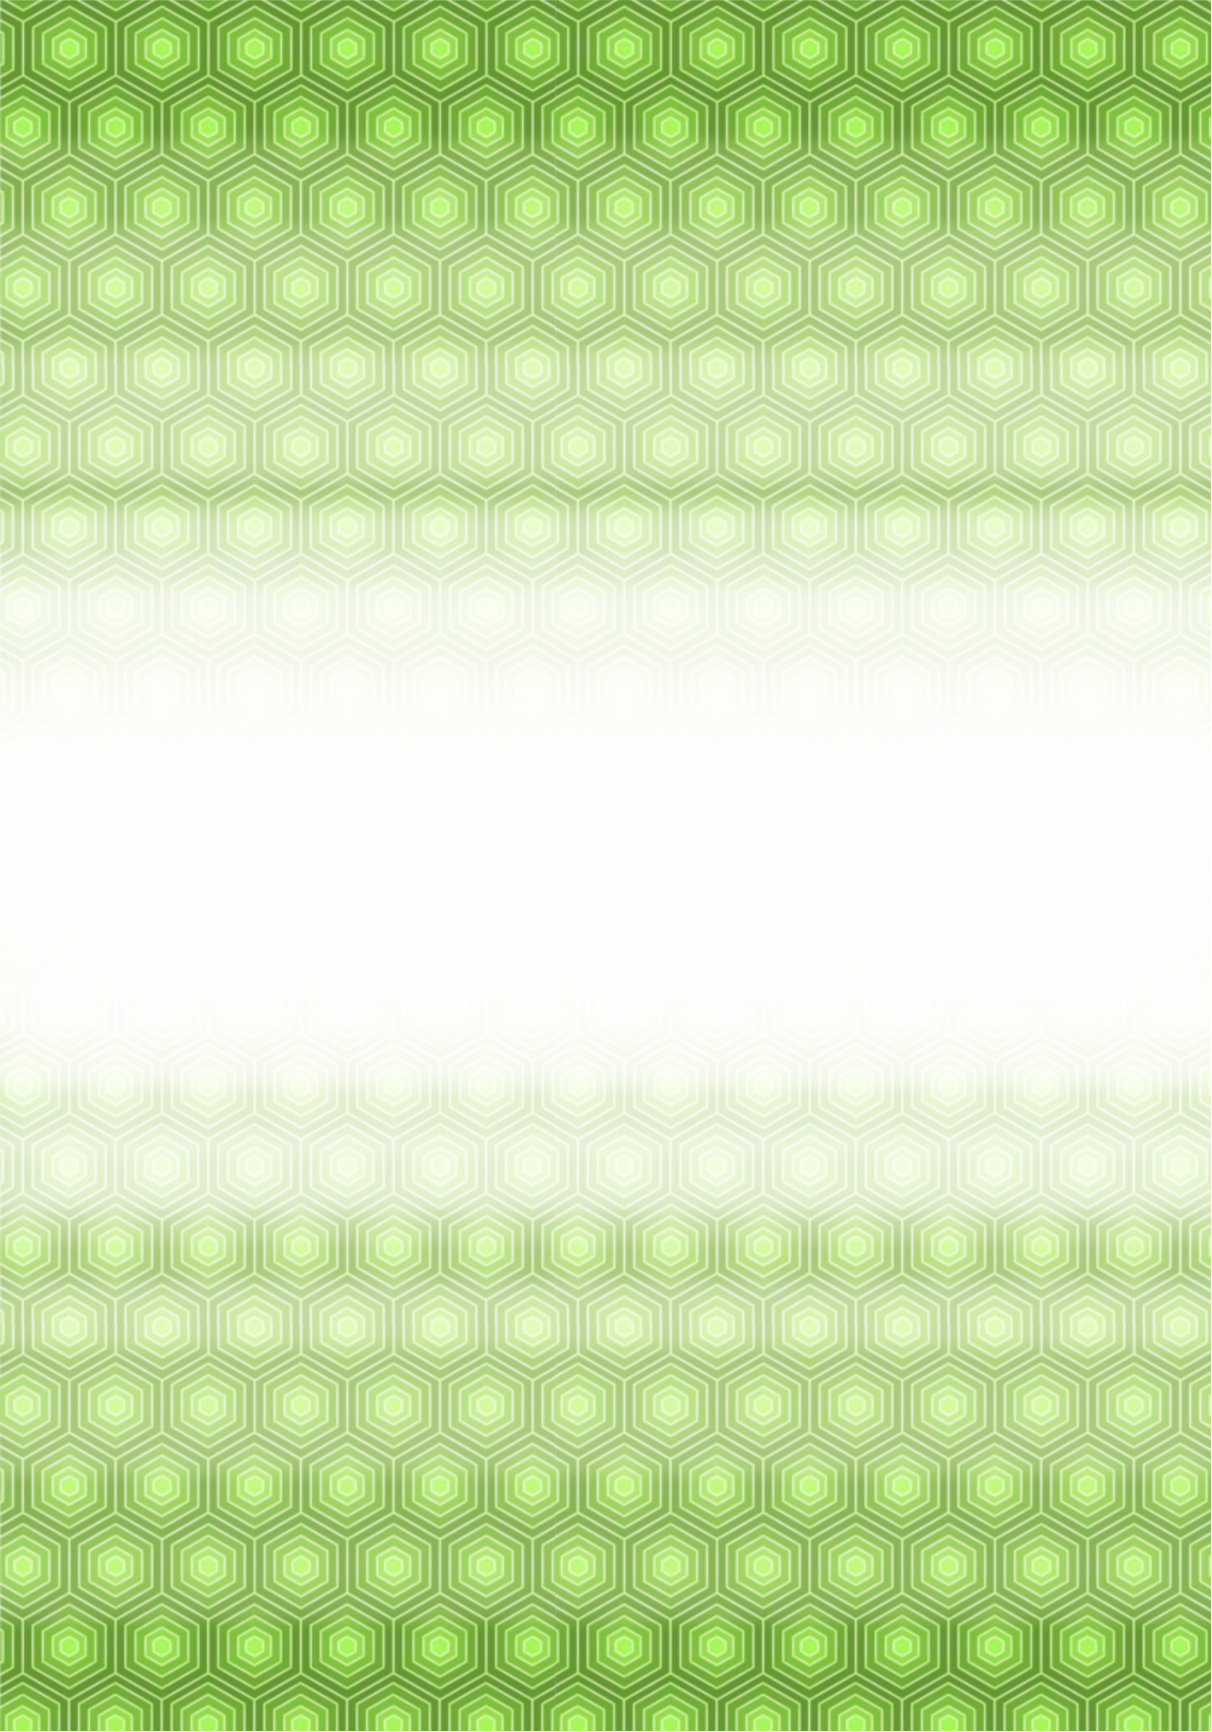
\includegraphics[scale=1]{cover}}} % Image background
\centering
\vspace*{3cm}
\begin{figure}[h]
\centering\hspace{30pt}
\includegraphics[scale=0.05]{turtle}
\end{figure}
\vspace*{1cm}
\par\normalfont\fontsize{50}{50}\sffamily\selectfont
로봇 프로그래밍\\
\textcolor{magenta}{\textbf{ROS}}로 시작하자!\par % Book title
{\Huge -로봇 운영 체제-}\\ % Sub book title
{\Huge \textit{(Robot Operating System)}}\par
\vspace*{6cm}
{\large 표윤석 지음}\par
{\large WWW.OROCA.ORG}\par
\endgroup

%-------------------------------------------------------------------------------
% COPYRIGHT PAGE
%-------------------------------------------------------------------------------

\newpage
~\vfill
\thispagestyle{empty}

\noindent 
로봇 프로그래밍 \textcolor{magenta}{\textbf{ROS}}로 시작하자!\\

\noindent Copyright \copyright\ 2014 by 표윤석 (Yoonseok Pyo, \href{mailto:passionvirus@gmail.com}{passionvirus@gmail.com})\\ % Copyright notice

\noindent \textsc{Published by OROCA (www.oroca.org)}\\ % Publisher

\noindent \textit{Ver 0.7, \today}\\ % Printing/edition date

\begin{figure}[h]

\includegraphics[scale=0.3]{cc-logo}
\hspace{10pt}

\includegraphics[scale=0.5]{by-nc}
\end{figure}

\noindent 이 저작물에는 크리에이티브 커먼즈 저작자표시 4.0 국제 라이선스가 적용 되어 있습니다. 이 라이선스의 설명을 보고 싶으시면 \url{http://creativecommons.org/licenses/by/4.0/} 을 참조하세요.\\

\noindent This work is licensed under the Creative Commons Attribution-NonCommercial 4.0 International License. To view a copy of this license, visit \url{http://creativecommons.org/licenses/by-nc/4.0/}. Unless required by applicable law or agreed to in writing, software distributed under the License is distributed on an \textsc{``as is'' basis, without warranties or conditions of any kind}, either express or implied. See the License for the specific language governing permissions and limitations under the License.\\ % License information

\noindent 이 저작물에서 사용된 (주)유진로봇의 Kobuki와 관련해서는 사용 허락을 받아 사용하였고, 본문에서 사용된 일부 이미지 및 템플릿에 대해서 별도의 라이선스를 가지고 있으며, 필자는 그 세부 사항을 아래에 표시합니다. 또한, 이 저작물에 사용된 이미지 중 CC BY-NC 이외의 저작권을 갖는 이미지는 각 페이지에 별도로 표시합니다.\\

\noindent Background image of cover page and chapter head image\\
Free Turtle Pattern By freecooldesign (www.freecooldesign.com)\\
License: CC BY-NC 3.0\\

\noindent Turtle image of cover page\\
By Nemo (http://pixabay.com/en/turtle-green-shell-animal-reptile-304427/)\\
License : CC0 Public Domain\\

\noindent LaTeX template ``The Legrand Orange Book'' made by LaTeXTemplates.com\\
Original author (LaTeX template): Mathias Legrand (legrand.mathias@gmail.com)\\
License: CC BY-NC-SA 3.0\\

\noindent \textbf{Also, We'd like to give special thanks to ROS development team, many ROS maintainers and contributors. We $\heartsuit$ ROS! (\url{http://www.ros.org/})}

%-------------------------------------------------------------------------------
% TABLE OF CONTENTS
%-------------------------------------------------------------------------------

\chapterimage{chapter_head_14.pdf} % Table of contents heading image

\pagestyle{empty} % No headers

\tableofcontents % Print the table of contents itself

\cleardoublepage % Forces the first chapter to start on an odd page so it's on the right

\pagestyle{fancy} % Print headers again

%-------------------------------------------------------------------------------
% CHAPTER  LIST
%-------------------------------------------------------------------------------

\setlength\parindent{1em}
%-------------------------------------------------------------------------------
\chapterimage{chapter_head_2.pdf} % Chapter heading image

%-------------------------------------------------------------------------------
\chapter{로봇 운영 체제}

%-------------------------------------------------------------------------------
\section{로봇 소프트웨어 플랫폼}\index{로봇 소프트웨어 플랫폼}

%-------------------------------------------------------------------------------
\subsection{플랫폼이 가져온 변화}\index{플랫폼이 가져온 변화}

잠깐, 로봇 이야기가 아닌, 핸드폰에 대해서 이야기해보자. 불가 20년전만 하더라도 스마트폰과 같은 핸드폰이 지금과 같이 많은 사람들의 필수품이 되리라고는 생각지도 못했었다.
더욱이, 초기의 핸드폰은 핸드폰이라는 이름이 무상할 정도로 크고 무거운 무전기와 같았고, 가격은 상상을 초월할 정도로 비쌌으며, 성능은 떨어졌다.
이에 비하여 현재의 스마트폰은 가격도 저렴하고, 가볍고, 작고 사용하기도 편리하다는 것을 본다면 그 변화는 놀랍기까지 하다.

올해 2013년, 40주년이 된 세계 최초의 상용 핸드폰인 모토롤라 다이나택 8000의 경우\footnote{http://www.segye.com/content/html/2013/04/04/20130404004829.html}\footnote{CarToyBlog, "Happy 40th Birthday to the Cell Phone!",  http://blog.cartoys.com/date/2013/04/},\footnote{http://venma.tistory.com/entry/Motorola-DynaTAC-8000X}, 그 당시 가격으로 500만원대, 0.8Kg의 무게, 최대 통화시간 30분, 충전 10시간 소요, 최대 30개 전화번호 입력 정도만이 가능하였다.
그 뒤로 핸드폰 시장은 급성장하게 되었고, 현재의 스마트폰까지 이르렀다. 그리고, 지금은 우리에게는 없어서는 안되는 생활 필수 아이템이 되었다.

그렇다면 이러한 것이 가능했던 이유는 무엇이였을까? 

초기에 많은 핸드폰 관련 회사들은 기술 경쟁을 거듭하며, 슬림하면서도 가볍고 고화질, 고음질, 휴대성 등 자신들만의 특징들을 네세우며 새로운 기기들을 내놓았다.
그 당시만해도 핸드폰은 모델마다 하드웨어에 맞게 기능을 추가하기 위하여 하드웨어 의존적인 펌웨어 개발을 했다.
한 회사에만 수 십가지 기종이 있었을테고, 전세계적으로는 어땠을까?
상상할 수도 없는 규모이다.
목적은 다 비슷한데 통합되지 못하고 그렇게 개발자들은 죽어라~ 새로운 하드웨어 개발 일정에 맞추어 펌웨어 개발을 했고 이는 반복되었다.
새로운 하드웨어마다 의존적으로 개발하였기에 그 발전 속도는 떨어졌고, 의존성으로 인하여 관리 비용은 높기만 했다.
그리고 그 비용은 우리 소비자의 몫이였다. 

지금은 어떠한가?
안드로이드, iOS, 윈도우즈 등 대표적인 OS를 기반으로 개발자들이 힘을 모으게 되었고 이러한 소프트웨어 플랫폼을 기반으로 핸드폰이라는 하드웨어 플랫폼을 잘 몰라도 관련 어플리케이션 개발에 문제가 없게 되었다.
그리고, 앱 개발자라는 새로운 소프트웨어 직종을 생길 정도로 스마트폰 운영체제를 기반으로 한 개발 환경이 확립되었으며, 스마트폰 운영체제 관리팀 이외에도 스마트폰 회사, 앱 개발자, 심지어 일반 사용자들까지도 하나로 뭉쳐서 하드웨어와 소프트웨어를 통합하는 플랫폼은 진화의 진화를 거듭하게 되었다.
이는 핸드폰 뿐만아니라 개인컴퓨터 개발과 더불어 불어닥친 유닉스, 리눅스, 윈도우, OS X 등의 컴퓨터용 OS 도 마찬가지 양상이라고 볼 수 있다.

이러한 이유로는 하드웨어의 급성장과 필연적인 사용자들의 수요도 있었겠지만,  소프트웨어 플랫폼 기반으로 지식이 한데 모아져서 나온 결과라고 볼 수 있다.
이러한 소프트웨어 플랫폼은 하드웨어 플랫폼의 인터페이스를 통합시키게 만들고, 나아가 하드웨어를 몰라도 상위 단의 프로그램인 응용 프로그램에 집중할 수 있게 되었기 때문에 사용자들의 수요에 맞는 응용 제품이 나올 수 있었다고 생각된다. 

%-------------------------------------------------------------------------------
\subsection{플랫폼이 가져온 변화}\index{플랫폼이 가져온 변화}

최근, 로봇계도 마찬가지의 움직임을 보이고 있다. 스마트폰 OS 나 개인컴퓨터 OS 에 비하여 그 규모는 작고, 아직 발전 단계이기는 하지만 로봇 소프트웨어 플랫폼은 춘추전국시대라고 볼 수 있을 정도로 매우 활발하게 진행되고 있다.
아래의 리스트는 그 중에서 돋보이는 활동을 보이고 있는 그룹들의 로봇 소프트웨어 플랫폼이다.

\begin{itemize}
\item ERSP,Evolution robotics (회사)\footnote{http://www.evolution.com/products/ersp/}
\item MSRDS,Microsoft (회사)\footnote{http://msdn.microsoft.com/en-us/robotics/default.aspx}
\item OpenRTM,일본의 AIST (국립 연구소)\footnote{http://www.openrtm.org}
\item ROS,Open Source Robotics Foundation\footnote{http://www.osrfoundation.org/}
\item OROCOS,유럽\footnote{http://www.orocos.org/}
\item OPRoS,한국\footnote{http://www.opros.or.kr/}
\end{itemize}

위와 같이 많은 플랫폼들이 등장하고 있고, 현재도 다양한 접근방식으로 증가 추세에 있다.
너도나도 로봇계의 로봇 소프트웨에 플랫폼의 선두에 서고 싶기 때문일 것이다.
현재, 다양한 로봇 소프트웨어 플랫폼이 나오고 있지만, 어느 것이 좋다라고는 섣불리 말하기 어려운게 사실이다.
그러나, 언젠가는 지금의 운영체제들처럼 독특한 스타일은 있을지는 몰라도 사용자 측면에서는 궁극적으로 비슷한 기능들로 압축 될 것이라고 생각한다.
우리는 소프트웨어 플랫폼 자체를 만드는 것이 아닌, 범용적인 로봇 소프트웨어 플랫폼에서도 돌아갈 수 있는 응용 프로그램 개발 능력에 집중하면 좋을 듯 싶다.
예를들어 안드로이드 어플 개발과 iOS 어플 개발이 비슷해진 것을 예를 들 수 있다. 

그렇다면 우리는 현재 나와있는 로봇 소프트웨어 플랫폼 중에서 어떤것을 우선적으로 익혀두면 좋을까?
필자는 이 중 어떤 것이 나에게 제일 적합하고, 앞으로 장래성이 있을까?
그리고 커뮤니케이션은?
오픈소스인가?
개발 환경은 어떻게 지원될까?
이러한 질문에서 가장 정답으로 생각하는 것은 Open Source Robotics Foundation 의 ROS라고 생각한다.
특히, 커뮤니티의 활발성, 준비되어 있는 라이브러리, 확장성, 개발 편의성을 생각해본다면 ROS 만한 것도 없어 보인다.
이 춘추전국시대와 같은 다양한 로봇 소프트웨어 플랫폼 중에서 어떤것이 살아 남을지 필자도 매우 궁금하다.

%-------------------------------------------------------------------------------
\subsection{로봇 소프트웨어 플랫폼이 가져올 미래}\index{로봇 소프트웨어 플랫폼이 가져올 미래}

로봇 소프트웨어 플랫폼은 정해진 하드웨어 플랫폼을 기준으로 하고 있기에 소프트웨어 플랫폼을 이용하면 하드웨어에 대한 지식이 없어도 응용 프로그램을 작성 가능하다.
이는 최신 스마트폰의 하드웨어 구성 및 세부 내역을 몰라도 어플을 작성가능한 것과 마찬가지이다.
또한, 로봇 개발자가 하드웨어 설계부터 소프트웨어 설계까지 하던 이전 작업 프로세서와 구별되어 더 많은 소프트웨어 인력들이 로봇 응용 제품에 참여 할 수 있다.
즉, 소프트웨어 플랫폼의 역할로 많은 이들이 로봇 개발에 동참하게 되는 길을 열고, 하드웨어는 소프트웨어 플랫폼을 사용하기 위하여 소프트웨어 플랫폼에서 제안하는 인터페이스에 맞도록 설계가 될것이다.
이는 로봇 개발이 급속도로 발전 할 수 있는 계기를 마련하게 되는 것이라고 생각한다.

%-------------------------------------------------------------------------------
\section{ROS 소개}\index{ROS 소개}

%-------------------------------------------------------------------------------
\subsection{ROS 란?}\index{ROS 란?}

ROS is an open-source, meta-operating system for your robot.
It provides the services you would expect from an operating system, including hardware abstraction, low-level device control, implementation of commonly-used functionality, message-passing between processes, and package management.
It also provides tools and libraries for obtaining, building, writing, and running code across multiple computers.

ROS 위키에는 위와 같은 정의를 내리고 있다. ROS는 로봇 응용프로그램을 개발할때 필요한 하드웨어 추상화, 하위 디바이스 제어, 일반적으로 사용되는 기능의 구현, 프로세스간의 메시지 패싱, 패키지 관리, 개발환경에 필요한 라이브러리와 다양한 개발 및 디버깅 도구를 제공한다는 것이다. 

즉, ROS는 로봇 응용 프로그램을 개발을 위한 운영체제와 같은 로봇 플랫폼이다.
이는 하드웨어 플랫폼을 하드웨어 추상화로 포함하고 있으며, 로봇 응용 소프트웨어 개발을 지원을 위한 소프웨어 플랫폼이면서 이기종의 하드웨어에서 사용 가능한 운영 체제와 같은 기능을 갖추고 있다.

%-------------------------------------------------------------------------------
\subsection{ROS는 새로운 운영체제(OS)인가?}\index{ROS는 새로운 운영체제(OS)인가?}

범용 컴퓨터의 경우, Windows(Windows XP, 7, 8 ...), Linux(Ubuntu, Fedora, Gentoo ...), MAC(OS X ...)가 있으며, 스마트폰의 경우에는 Android, iOS, Symbian, RiMO, Bada 등 많은 OS가 있다.
모두 전통적인 OS(Operating System)에 속하게 된다.
정말 다양한 하드웨어에 수 많은 OS의 종류가 있다. 

ROS는 Robot Operating System 이라고 하여 OS 임을 나태내고 있다.
특히, ROS를 처음 접한 사람들은 ROS를 전통적인 운영체제라고 생각하는 경우가 있다.
필자 역시, 처음에는 ROS가 로봇을 위한 새로운 운영체제라고 생각하였다. 

그러나, No!, ROS은 메타운영체제(Meta-Operating System)이다.

메타운영체제(Meta-Operating System) 딱히 정확히 정의된 용어는 아니지만, 어플리케이션과 분산 컴퓨팅 자원간의 가상화 레이어로 분산 컴퓨팅 자원을 활용하여, 스케쥴링 및 로드, 감시, 에러 처리 등을 실행하는 시스템이라고 볼 수 있다.
즉, 윈도우, 리눅스, 안드로이드와 같은 전통적인 운영체제는 아니다.
오히려, ROS는 기존의 전통적인 운영체제(리눅스,윈도우,OS-X,안드로이드)를 이용하고 있다.
리눅스의 한 배포판인 Ubuntu과 같은 운영체제의 프로세스 관리 시스템, 파일 시스템, 유저 인터페이스, 프로그램 유틸(컴파일러, 스레드 모델 등)등을 사용하고 있다.
이에 추가적으로 다수의 이기종 하드웨어간의 데이터 송수신, 스케쥴링, 에러 처리 등 로봇 응용 소프트웨어에 필요한 필수 기능들을 라이브러리 형태로 제공하고 있다.
또한, 이러한 기반 로봇 프레임워크를 기반으로 다양한 목적의 응용 패키지를 개발, 관리, 제공하고 있으며 유저들이 개발한 패키지 또한 유통하는 생태계(ecosystem)를 갖추고 있다.

또한, 아래의 그림처럼 ROS는 하나의 운영체제에서의 메시지도 지원하지만 서로 다른 운영체제, 하드웨어, 프로그램에서도 메시지 처리를 할 수가 있어서 다양한 하드웨어가 이용되는 로봇 개발에는 매우 적합한 운영체제라고 할 수 있다.
이에 대한 내용은 이어지는 강좌들에서 좀 더 자세히 다루기로 하겠다.  

그림으로 나타내면 아래와 같다고 볼 수 있다. 기존의 전통적인 운영체제를 이용하면서, 로봇 응용 개발에 필수적인 로봇 및 센서의 하드웨어 추상화 개념으로 이를 제어하고, 유저의 로봇 응용 프로그램 개발을 위한 지원 시스템인것이다.

%-------------------------------------------------------------------------------
\subsection{ROS 생태계}\index{ROS 생태계}

스마트폰 시장에서 Android, iOS,  Symbian, RiMO, Bada 등 다양한 OS가 등장하면서 생태계(ecosystem)라는 말을 자주 듣곤 한다.
이는 스마트폰을 생산하는 하드웨어 회사와 이를 사용하는 유저 혹은 어플리케이션 소프트웨어(앱,APP) 개발자를 연결해주는 구조를 말한다.
스마트폰 회사들이 기기를 생산, 운영체제의 인터페이스에 맞추고, 각 OS 회사들은 이를 라이브러리화시켜 제공해주고, 소프트웨어 개발자들이 이를 이용하여 하드웨어 지식이 없어도 손쉽게 개발작업을 해줄 수 있는 구조, 그리고 유저가 사용하기 쉽도록 유통하는 것이 바로 생태계이다. 

이러한 생태계는 모바일 시장에서 제일 먼저 했던것은 아니다.
범용 컴퓨터 분야도 다양한 하드웨어 회사들이 있고, 이를 묶어준 것은 마이크로소프트사의 Windows OS 및 자유진영의 리눅스가 대표적이였다.
어쩜 이러한 흐름은 자연의 생태계처럼 비슷한 흐림이 아닐까 싶다. 

로봇 분야도 마찬가지 흐름으로 가고 있다.
처음에는 여러 시도로 각종 하드웨어 기술들이 넘쳐흘렀으나, 이를 통합해줄 OS가 전무했다.
이 상황에서 다양한 소프트웨어 플랫폼이 등장했고, 가장 주목받은 ROS의 경우 이제 그 생태계의 틀을 갖추기 시작했다.
아직, 그 여파력은 미미하지만 점점 늘고 있고 있는 유저들과 회사들 그리고 급격히 늘고 있는 관련 툴 및 라이브러리를 볼 때 멀지 않아 생태계가 완만히 돌아갈 것이라고 기대해본다.
그리고, 로봇회사 및 센서회사와 같은 로봇 관련 하드웨어 분야의 개발자, ROS 개발 운용 팀, 응용 소프트웨어 개발자, 유저 모두가 웃을 수 있는 생태계가 되길 바란다.
 
아래는 2013년 9월 기점으로 필자가 조사해본 ROS 실태이다.
아직, 미미한 수준이라고 생각하는 사람들도 있지만, 로봇 분야에서 이만큼 세력을 키운 로봇 소프트웨어 플랫폼은 없다고 생각한다.
앞으로 어떻게 변할지 점점 기대가 된다!

% \begin{enumerate}
% \item The first item
% \item The second item
% \item The third item
% \end{enumerate}

% \subsection{Bullet Points}\index{Lists!Bullet Points}

% \begin{itemize}
% \item The first item
% \item The second item
% \item The third item
% \end{itemize}

% \subsection{Descriptions and Definitions}\index{Lists!Descriptions and Definitions}

% \begin{description}
% \item[Name] Description
% \item[Word] Definition
% \item[Comment] Elaboration
% \end{description}
% -*- root: main.tex -*-
%-------------------------------------------------------------------------------
\chapterimage{chapter_head_2.pdf} 

%-------------------------------------------------------------------------------
\chapter{ROS 설치 (일반PC)}

%-------------------------------------------------------------------------------
\section{ROS Indigo 설치}\index{ROS Indigo 설치}

%-------------------------------------------------------------------------------
\subsection{개발 환경}\index{개발 환경}

ROS 개발 환경에 대해서 알아보기로 하자. ROS는 Ubuntu, OS X, Windows, Fedora, Gentoo, OpenSUSE, Debian, Arch Linux 등을 지원하고 있지만 우분투(Ubuntu) 를 제외 하고는 공식적으로 지원하는 것이 아닌 설치 방법만 언급하고 있다. 하지만, 우분투 이외의 주요 운영 체제인 OS X, Windows 는 유저들이 많은 편이라 어느 정도 만족스럽게 쓸 수 있을 것이다. 우분투 버전이 다른 경우에는 공식 페이지\footnote{\url{http://wiki.ros.org/indigo/Installation/Ubuntu}}를 보기를 권하며, OS X\footnote{\url{http://wiki.ros.org/indigo/Installation/OSX/Homebrew/Source}}, Windows\footnote{\url{http://wiki.ros.org/hydro/Installation/Windows}}의 경우에는 각각의 설치 방법을 관련 위키\footnote{ROS 위키, 환경 설정, \url{http://wiki.ros.org/ROS/Tutorials/InstallingandConfiguringROSEnvironment}}\footnote{ROS 위키, catkin 빌드 시스템, \url{http://wiki.ros.org/catkin}}에서 확인하기 바란다. 여기서는 우분투에 대해서만 언급하겠다. 그리고 INTEL 및 AMD CPU가 아닌 ARM CPU등을 사용하는 SBC(Single Board Computer)의 경우에는 챕터\ref{cha:ros_install_sbc}에서 자세히 다루도록 하겠다.
\\
\begin{itemize}
\item 하드웨어: INTEL 및 AMD 칩을 사용하는 데스크톱 및 노트북 
\item 운영체제: Ubuntu 14.04 LTS (Trusty Tahr)
\item ROS: Indigo Igloo
\end{itemize}

\begin{figure}[h]
\centering
\includegraphics[height=35mm]{pictures/chapter2/ubuntu_14_04.jpg}
\centering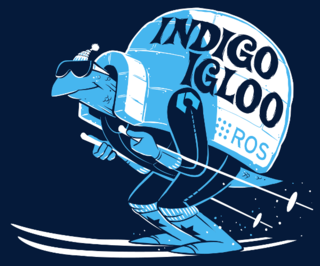
\includegraphics[height=35mm]{pictures/chapter2/indigo_igloo.png}
\caption{우분투 Trusty 버전과 ROS Indigo 버전의 로고}
\end{figure}

%-------------------------------------------------------------------------------
\subsection{ROS Indigo 설치 방법}\index{ROS Indigo 설치 방법}
\label{sec:ROSInstallation}

\begin{exercise}[간단 설치]
아래의 강좌보다 간단히 설치 할 수 있는 스크립트를 이용한 설치 방법은 섹션\ref{sec:SimpleInstallation}[ROS Indigo 간단 설치]을 참조하기 바란다.\\
\end{exercise}

%-------------------------------------------------------------------------------
\subsubsection{NTP (Network Time Protocol) 설정}
ROS 공식 설치 항목에는 포함되어 있지는 않지만 NTP 설정을 해주자.이는 서로 다른 PC간의 통신에서 ROS Time 의 오차를 줄일 수 있다. 설정법은 매우 간단하여 아래의 명령어처럼 우선 chrony 를 설치한 후, ntpdate 이라는 명렁어로 ntp 서버를 지정하면 된다. 결과, 서버측과의 현재 컴퓨터 시간 오차를 표시해주며, 설정한 서버 시간에 맞추게 될 것이다. 이는 서로 다른 PC 간에 같은 NTP 서버를 지정함으로써 시간 오차를 최소한으로 줄이는 방법이라 할 수 있다.
\\
\begin{lstlisting}[language=ROS]
$ sudo apt-get install chrony
$ sudo ntpdate ntp.ubuntu.com
\end{lstlisting}

%-------------------------------------------------------------------------------
\subsubsection{소스 리스트 추가}
sources.list 에 ROS 저장소 주소를 추가하자. 새로운 커맨드 창을 열고 아래와 같이 입력한다.
\\
\begin{lstlisting}[language=ROS]
$ sudo sh -c 'echo "deb http://packages.ros.org/ros/ubuntu trusty main" > /etc/apt/sources.list.d/ros-latest.list'
\end{lstlisting}

%-------------------------------------------------------------------------------
\subsubsection{키 설정}
ROS 저장소로부터 패키지를 다운로드 받기 위해 공개키를 추가하자. 아래와 같이 입력한다.
\\
\begin{lstlisting}[language=ROS]
$ wget https://raw.githubusercontent.com/ros/rosdistro/master/ros.key -O - | sudo apt-key add -
\end{lstlisting}

%-------------------------------------------------------------------------------
\subsubsection{패키지 인덱스 업데이트}
소스 리스트에 ROS 저장소 주소를 넣었으니 패키지 리스트를 다시 재인덱싱을 하고, 설치에 있어서 필수 사항은 아니지만 ROS 설치 전에 현재 설치된 우분투 관련 모든 패키지를 판올림 하기를 추천한다.
\\
\begin{lstlisting}[language=ROS]
$ sudo apt-get update && sudo apt-get upgrade
\end{lstlisting}

%-------------------------------------------------------------------------------
\subsubsection{ROS Indigo Igloo 설치}
이 명령어로 데스크톱용 기본적인 ROS 패키지들을 설치하게 된다. 여기에는 ROS, rqt, rviz, 로봇 관련 라이브러리, 시뮬레이션, 네이게이션 등이 포함되어 있다.
\\
\begin{lstlisting}[language=ROS]
$ sudo apt-get install ros-indigo-desktop-full
\end{lstlisting}

필자의 경우에는 추가로 rqt 관련 패키지를 설치하고 있다. 위의 설치만으로도 기본적인 rqt는 포함되지만 아래의 설치로 rqt관련 모든 패키지를 설치하는것이 여러모로 편하고, 다양한 rqt 플러그인을 사용가능해진다.
\\
\begin{lstlisting}[language=ROS]
$ sudo apt-get install ros-indigo-rqt-*
\end{lstlisting}

만약, 그 이외에 패키지를 설치하고 싶은 경우에는 아래와 같이 apt-cache 의 명령어를 이용하여 ros-indigo 로 시작되는 패키지들을 검색할 수 있다. 현재 아래의 명령어를 실행해보면 대략 900여개의 패키지를 확인할 수 있다. 패키지 개별 설치를 원하는 경우에는 sudo apt-get install ros-indigo-[패키지이름] 과 같은 명령어로 개별 패키지를 설치 가능하다. 그 이외에 GUI 툴인 sysnaptic package manager 를 이용해도 된다.

\begin{exercise}[APT (Advanced Packaging Tool)]
apt-get, apt-key, apt-cache 등에 나오는 apt는 Advanced Packaging Tool 이라고 하여서 우분투(Ubuntu)를 포함안 데비안(Debian)계열의 리눅스에서 많이 사용하는 패키지 관리 명령어이다\footnote{\url{http://en.wikipedia.org/wiki/Advanced_Packaging_Tool}}.
\end{exercise}

\begin{exercise}[패키지 검색 방법]
apt-cache search ros-indigo
\end{exercise}

\begin{exercise}[패키지 개별 설치 방법]
sudo apt-get install ros-indigo-패키지이름
\end{exercise}

\begin{exercise}[이전 버전의 ROS 삭제 및 번갈아 가며 사용하기]
아래의 명령어로 설정과 파일을 같이 삭제 가능하다. 만약, 기존 버전과 함께 사용하고자하는 경우에는 설정파일을 불러오는 명령어중 source /opt/ros/indigo/setup.bash 의 부분을 indigo 또는 hydro 로 바꾸면 된다. sudo apt-get purge ros-hydro-*
\end{exercise}

%-------------------------------------------------------------------------------
\subsubsection{rosdep 초기화}
ROS를 사용하기 전에 rosdep 를 초기화해주어야만 한다. rosdep 는 ros의 핵심 컴포넌트들을 사용하거나 컴파일 할때 의존성 패키지를 쉽게 설치하여 사용자 편의성을 높인 기능이다.
\\
\begin{lstlisting}[language=ROS]
$ sudo rosdep init
$ rosdep update
\end{lstlisting}

%-------------------------------------------------------------------------------
\subsubsection{rosinstall 설치}
ROS의 다양한 패키지를 인스톨하는 프로그램이다. 빈번하게 사용할 정도로 유용한 도구인 만큼 꼭 설치하자. 
\\
\begin{lstlisting}[language=ROS]
$ sudo apt-get install python-rosinstall
\end{lstlisting}

%-------------------------------------------------------------------------------
\subsubsection{환경설정 파일 불러오기}
환경 설정이 설정되어 있는 파일을 불러온다. ROS\_ROOT, ROS\_PACKAGE\_PATH 등의 환경 변수들이 정의되어 있다.
\\
\begin{lstlisting}[language=ROS]
$ source /opt/ros/indigo/setup.bash
\end{lstlisting}

%-------------------------------------------------------------------------------
\subsubsection{작업폴더 생성 및 초기화}
ROS에서는 catkin 이라는 ROS 전용 빌드 시스템을 사용하고 있다. 이를 사용하기 위해서는 아래와 같이 catkin 작업 폴더 및 작업 폴더 초기화 설정을 해주어야 한다. (아래의 설정은 ROS를 사용함에 있어서 처음 한 번만 해주면 된다.)
\\
\begin{lstlisting}[language=ROS]
$ mkdir -p ~/catkin_ws/src
$ cd ~/catkin_ws/src
$ catkin_init_workspace
\end{lstlisting}

catkin 작업 폴더를 생성하였으면 컴파일을 하자. 현재의 catkin 작업 폴더에는 src 폴더 및 그 안의 CMakeLists.txt 이외에 아무런 파일이 없지만 시험삼아 아래와 같이 catking\_make 명령어를 이용하여 빌드하여 보자. 
\\
\begin{lstlisting}[language=ROS]
$ cd ~/catkin_ws/
$ catkin_make
\end{lstlisting}

문제없이 빌드를 마치게 되면 아래와 같이 ls 명령어를 실행해보자. 유저가 직접 생성하였던 src 폴더 이외의 없었던 build 및 devel 폴더가 새로 생성되었을 것이다. catkin 빌드 시스템의 빌드 관련 파일은 build 폴더에, 빌드 후 실행관련 파일은 devel 폴더에 저장된다.
\\
\begin{lstlisting}[language=ROS]
$ ls
build  devel  src
\end{lstlisting}

마지막으로, catkin 빌드 시스템과 관련된 환경 파일을 불러오자. 
\\
\begin{lstlisting}[language=ROS]
$ source ~/catkin_ws/devel/setup.bash
\end{lstlisting}

%-------------------------------------------------------------------------------
\subsection{테스트}\index{테스트}

ROS의 모든 설치가 완료되었다. 마지막으로, 제대로 설치가 되었는지 테스트하기 위하여 지금의 모든 터미널창을 닫고, 새 터미널 창을 실행하자. 그 다음 아래의 명령어를 입력하여 roscore 를 실행해보자.
\\
\begin{lstlisting}[language=ROS]
$ roscore
\end{lstlisting}

\noindent
아래와 같이 에러가 없이 실행되었다면 설치가 완료된 것이다. 종료는 Ctrl-c 이다.
\\
\begin{lstlisting}[language=ROS]
... logging to /home/xxx/.ros/log/35c1e494-8097-11e4-a84a-d43d7e970cb0/roslaunch-xxx-23589.log
Checking log directory for disk usage. This may take awhile.
Press Ctrl-C to interrupt
Done checking log file disk usage. Usage is <1GB.

started roslaunch server http://192.168.4.100:51518/
ros_comm version 1.11.9


SUMMARY
========

PARAMETERS
 * /rosdistro: indigo
 * /rosversion: 1.11.9

NODES

auto-starting new master
process[master]: started with pid [23601]
ROS_MASTER_URI=http://192.168.4.100:11311/

setting /run_id to 35c1e494-8097-11e4-a84a-d43d7e970cb0
process[rosout-1]: started with pid [23614]
started core service [/rosout]
\end{lstlisting}

%-------------------------------------------------------------------------------
\section{ROS Indigo 간단 설치}\index{ROS Indigo 간단 설치}
\label{sec:SimpleInstallation}

자신이 사용중인 우분투 버전이 13.04, 14.04 이라면 앞서 설명한 ROS 설치를 간단히 수행하는 스크립트를 만들어 두었다. 이를 이용하면 비교적 손쉽게 설치 할 수 있다.
\\
\begin{lstlisting}[language=ROS]
$ wget https://raw.githubusercontent.com/oroca/oroca-ros-pkg/master/ros_indigo_install.sh
$ sh ros_indigo_install.sh
\end{lstlisting}

%-------------------------------------------------------------------------------
\section{ROS Indigo 설치 (간략버전)}\index{ROS Indigo 설치 (간략버전)}

아래의 명령어들은 챕터\ref{sec:ROSInstallation} ROS의 Indigo 버전 설치의 요약판이다. 긴 설명 없이 바로 설치하실 분들에게 도움이 될 것이다. ※ xxx.xxx.xxx.xxx 는 자신의 IP 주소를 입력하면 된다.

\begin{lstlisting}[language=ROS]
$ sudo apt-get install chrony
$ sudo ntpdate ntp.ubuntu.com
$ sudo sh -c 'echo "deb http://packages.ros.org/ros/ubuntu trusty main" > /etc/apt/sources.list.d/ros-latest.list'
$ wget https://raw.githubusercontent.com/ros/rosdistro/master/ros.key -O - | sudo apt-key add -
$ sudo apt-get update
$ sudo apt-get upgrade
$ sudo apt-get install ros-indigo-desktop-full
$ sudo apt-get install ros-indigo-rqt-*
$ sudo rosdep init
$ rosdep update
$ echo "source /opt/ros/indigo/setup.bash" >> ~/.bashrc
$ source ~/.bashrc
$ sudo apt-get install python-rosinstall
$ mkdir -p ~/catkin_ws/src
$ cd ~/catkin_ws/src
$ catkin_init_workspace
$ cd ~/catkin_ws/
$ catkin_make
$ echo "source ~/catkin_ws/devel/setup.bash" >> ~/.bashrc
$ echo "export ROS_MASTER_URI=http://xxx.xxx.xxx.xxx:11311" >> ~/.bashrc
$ echo "export ROS_HOSTNAME=xxx.xxx.xxx.xxx" >> ~/.bashrc
$ source ~/.bashrc
\end{lstlisting}

%-------------------------------------------------------------------------------
\section{ROS 개발 환경 구축 (환경설정)}\index{ROS 개발 환경 구축 (환경설정)}

%-------------------------------------------------------------------------------
\subsection{환경 설정}\index{환경 설정}

ROS 설치 과정에서 사용된 다음 명렁어처럼 환경 설정 파일을 불러오는 것은 새로운 터미널 창을 열때마다 매번 실행 해줘야 한다. 이러한 번거로운 작업을 없애기 위하여 새로운 터미널 창을 열때마다 정해진 환경 설정 파일을 읽어오도록 설정해주도록 하자. 그 이외에도 ROS 네트워크 설정 및 자주 사용하는 명령어를 단축 명령어도 설정하도록 하자.
\\
\begin{lstlisting}[language=ROS]
$ source /opt/ros/indigo/setup.bash
$ source ~/catkin_ws/devel/setup.bash
\end{lstlisting}

우선, gedit 프로그램과 같은 문서편집 프로그램을 사용하여 bashrc 파일을 수정하도록 하자. 아래의 명령어로 bashrc 파일을 불러오자. 이 책에서는 모든 챕터에 걸쳐서 문서폅집에 gedit을 사용하였지만 gedit가 아니더라도 sublime text, vim, emacs, nano 등을 사용해도 무방하다.
\\
\begin{lstlisting}[language=ROS]
$ gedit ~/.bashrc
\end{lstlisting}

bashrc 파일을 불러오면 이미 매우 많은 설정들이 있을 것이다. 이전 설정들은 건들지 말고, bashrc 파일의 제일 하단으로 내려가서 아래의 내용을 추가해주도록 하자. (xxx.xxx.xxx.xxx 는 자신의 IP이다.)
\\
\begin{lstlisting}[language=bash]
# Set ROS Indigo
source /opt/ros/indigo/setup.bash
source ~/catkin_ws/devel/setup.bash
# Set ROS Network
export ROS_MASTER_URI=http://xxx.xxx.xxx.xxx:11311
export ROS_HOSTNAME=xxx.xxx.xxx.xxx
# set ROS alias command
alias cw='cd ~/catkin_ws'
alias cs='cd ~/catkin_ws/src'
alias cm='cd ~/catkin_ws && catkin_make'
\end{lstlisting}

위 설정 이외에 필자는 아래와 같은 추가 설정을 하기도 한다. 아래의 내용은 어디까지나 참고 사항이니 설정하지 않아도 된다.
\\
\begin{lstlisting}[language=bash]
# Set User Alias
alias rm='rm -rf' 
alias eb='gedit ~/.bashrc' 
alias sb='source ~/.bashrc'
alias agi='sudo apt-get install'  
alias m='make -j4 -l4'  
alias gs='git status'  
alias gp='git pull'
alias catkin_eclipse='catkin_make --force-cmake -G"Eclipse CDT4 - Unix Makefiles"'
\end{lstlisting}

\noindent
다음으로는 위에서 설정한 내용들에 대하여 좀 더 자세히 설명하도록 하겠다.

%-------------------------------------------------------------------------------
\subsubsection{ROS 환경 설정 불러오기}
\# 은 주석문이 시작된다는 것을 알리는 문법이고 그 뒤의 내용이 주석문이다. 그리고, 2번째 줄의 source/opt/ros/indigo/setup.bash 및 3번째 줄의 source $\sim$/catkin\_ws/devel/setup.bash 은 필수로 설정해줘야 하는 ROS 환경 설정 파일이다.
\\
\begin{lstlisting}[language=bash]
# set ROS Indigo
source /opt/ros/indigo/setup.bash
source ~/catkin_ws/devel/setup.bash
\end{lstlisting}

%-------------------------------------------------------------------------------
\subsubsection{ROS 네트워크 설정}
ROS\_MASTER\_URI 와 ROS\_HOSTNAME 의 설정이다. ROS는 네트워크를 이용하여 노드간에 메시지 통신을하기 때문에 이 설정이 중요하다. 우선은 둘다 자신의 네트워크 IP를 입력해주면 된다. 차후에 마스터 PC가 따로 있고, 로봇은 호스트 PC를 사용하는 경우, 이를 구분하여 입력하면 서로 다른 컴퓨터간의 통신이 가능하게 된다. 지금은 둘다 모두 자신의 네트워크 IP를 입력해주자. 아래의 예제는 IP가 192.168.4.100 인 경우의 설정예이다. 
\\
\begin{lstlisting}[language=bash]
# set ROS Network
export ROS_MASTER_URI=http://192.168.4.100:11311
export ROS_HOSTNAME=192.168.4.100
\end{lstlisting}

\begin{exercise}[ifconfig]
리눅스에서 자신의 IP를 알아보는 방법으로는 ifconfig 명령어를 이용하는 방법이 제일 간단하다. 아래의 예제처럼 터미널창에서 ifconfig를 실행해보자. 유선이라면 eth, 무선이라면 wlan 의 항목의 inet addr 부분의 IP가 자신의 IP이다. 필자의 경우, 유선랜을 이용하지만 일부로 무선랜도 켜보았다. 아래의 예제에서의 유선 접속시의 IP는 192.168.4.100 이다.
\begin{lstlisting}[language=ROS, backgroundcolor=\color{ocre!10}, numbers=none]
$ ifconfig
eth0   Link encap:Ethernet  HWaddr xx:xx:xx:xx:xx:xx  
          inet addr:%*\textbf{\textcolor{red}{192.168.4.100}}*)  Bcast:192.168.4.255  Mask:255.255.255.0
          inet6 addr: fexx::d6xx:7exx:f1xx:xx2/64 Scope:Link

lo       Link encap:Local Loopback  
          inet addr:127.0.0.1  Mask:255.0.0.0
          inet6 addr: ::1/128 Scope:Host

wlan1 Link encap:Ethernet  HWaddr xx:xx:xx:xx:xx:xx
          inet addr:192.168.4.200  Bcast:192.168.4.255  Mask:255.255.255.0
          inet6 addr: fexx::23xx:dfxx:fexx:5exx/64 Scope:Link
\end{lstlisting}
\end{exercise}

%-------------------------------------------------------------------------------
\subsubsection{단축 명령어}
ROS 개발 작업에서 자주 사용하는 명령어를 단축 명령어로 설정하는 방법에 대해서 알아보도록 하자. 아래의 cw, cs, cm 은 필자가 만들어둔 단축 명령어이다. 이 단축 명령어는 리눅스에서 사용하는 alias 라는 단축 명령어를 이용하여 작성하였다.\\

\begin{itemize}[leftmargin=*]
\item cw 는 미리 설정해 둔 catkin 작업 폴더인 ~/catkin\_ws 로 이동한다. 
\item cs 는 catkin 작업 폴더 중 소스 파일이 담겨있는 ~/catkin\_ws/src 로 이동한다. 
\item cm 는 catkin 작업 폴더인 ~/catkin\_ws 로 이동한 후, catkin\_make 명령어로 ROS 패키지를 빌드하게 된다.
\end{itemize}

\vspace{\baselineskip}
\begin{lstlisting}[language=bash]
# set ROS alias command
alias cw='cd ~/catkin_ws'
alias cs='cd ~/catkin_ws/src'
alias cm='cd ~/catkin_ws && catkin_make'
\end{lstlisting}

\begin{exercise}[ROS 환경 설정 확인 방법]
아래처럼 export \textbar~grep ROS 명령어를 이용하여 자신이 현재 설정한 ROS 환경 설정들을 확인할 수 있다.
\begin{lstlisting}[language=bash, backgroundcolor=\color{ocre!10}, numbers=none]
$ export | grep ROS
declare -x ROSLISP_PACKAGE_DIRECTORIES="/home/xxx/catkin_ws/devel/share/common-lisp"
declare -x ROS_DISTRO="indigo"
declare -x ROS_ETC_DIR="/opt/ros/indigo/etc/ros"
declare -x ROS_HOSTNAME="192.168.4.100"
declare -x ROS_MASTER_URI="http://192.168.4.100:11311"
declare -x ROS_PACKAGE_PATH="/home/xxx/catkin_ws/src:/opt/ros/indigo/share:/opt/ros/indigo/stacks"
declare -x ROS_ROOT="/opt/ros/indigo/share/ros"
declare -x ROS_TEST_RESULTS_DIR="/home/xxx/catkin_ws/build/test_results"
\end{lstlisting}
\end{exercise}

%-------------------------------------------------------------------------------
\section{ROS 개발 환경 구축 (IDE)}\index{ROS 개발 환경 구축 (IDE)}

%-------------------------------------------------------------------------------
\subsection{통합 개발 환경 (Integrated Development Environment, IDE)}

IDE는 코딩, 디버그, 컴파일, 배포 등 프로그램 개발에 관련된 모든 작업을 하나의 프로그램 안에서 처리하는 환경을 제공하는 소프트웨어를 말한다. 아마 많은 개발자들이 자신만이 즐겨쓰는 IDE는 한두 개쯤은 있을 것으로 생각한다. 

ROS 또한 여러 IDE\footnote{ROS 위키, IDEs, \url{http://wiki.ros.org/IDEs}}를 사용할 수 있는데, 많이 사용되는 IDE로는 Eclipse, CodeBlocks, Emacs, Vim, NetBeans, QtCreator 등이 있다. 필자의 경우, 처음에는 Eclipse 를 사용 하였으나 Eclipse가 최근 버전에 와서는 매우 무겁게 느껴졌으며, ROS의 catkin 빌드 시스템 사용에 있어서 많은 불편을 느꼈다. 그래서, 다른 IDE 를 구축하고자 여러 IDE 를 검토해 봐다. 그 중 가장 적합한 툴로는 QtCreator\footnote{Qt Project, \url{http://qt-project.org/}}\footnote{Qt Download page, \url{http://qt-project.org/downloads}}가 아닐까 싶다. ROS 의 개발/디버깅 툴인 rqt 같은 경우나, RViz 같은 경우에도 Qt로 만들어져 있고, 사용자는 Qt 플러그인으로 기존 툴과 플러그인을 개발도 가능하다는 점에서 Qt의 편집기인 QtCreator 는 매우 유용하다고 볼 수 있다. 또한 Qt 를 이용하지 않더라도 범용적인 에디터로써의 기능도 충분히 갖추고 있을뿐 아니라, 프로젝트를 CMakeLists.txt 를 통하여 바로 불러올 수 있어서 catkin\_make 사용에 있어서 매우 편리하다.

아래의 내용은 QtCreator 로 ROS 개발 환경을 꾸미는 내용을 담고 있다. 반드시 QtCreator 를 이용하여 개발할 필요는 없으므로 QtCreator 를 IDE로 사용하지 않더라도 뒤에 따르는 내용을 이해하는 데에는 아무런 문제가 없음을 미리 밝혀둔다.

%-------------------------------------------------------------------------------
\subsubsection{QtCreator 설치}

\vspace{\baselineskip}
\begin{lstlisting}[language=ROS]
$ sudo apt-get install qtcreator
\end{lstlisting}

%-------------------------------------------------------------------------------
\subsubsection{QtCreator 구동}
QtCreator를 아이콘으로 실행시켜도 구동에는 문제 없으나 우리가 \textasciitilde/.bashrc 에 기술해둔 ROS 경로 등의 설정을 QtCreator 에도 적용하기 위해서는 새로운 터미널 창을 열어, 아래와 같이 실행해줘야 한다. 즉, QtCreator 를 실행할때 환경 설정 파일인 \textasciitilde/.bashrc 에 기술해 놓은 설정을 모두 적용하게 된다.\\

\begin{lstlisting}[language=ROS]
$ qtcreator
\end{lstlisting}

\noindent
위의 명령어로 아래와 같이 QtCreator 가 실행됨을 확인 할 수 있다.

\begin{figure}[h]
\centering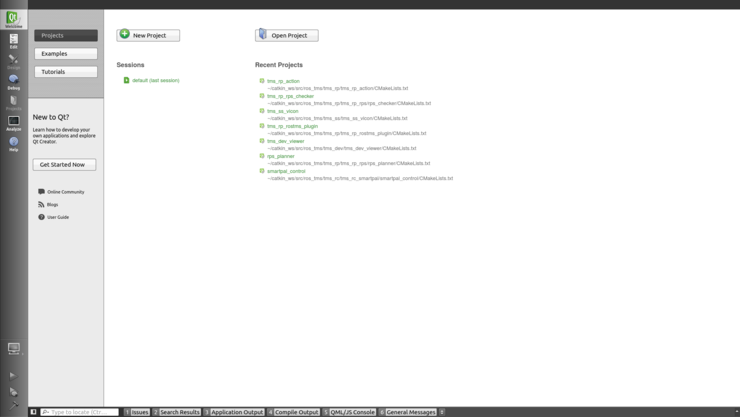
\includegraphics[width=0.9\columnwidth]{pictures/chapter2/qtcreator1.png}
\caption{QtCreator IDE}
\end{figure}

%-------------------------------------------------------------------------------
\subsubsection{ROS 패키지를 프로젝트로 불러오기}
앞서 말한바와 같이 QtCreator는 기본적으로 CMakeLists.txt 를 사용하고 있고, ROS 패키지도 CMakeLists.txt 기반이기에 단순히 아래와 화면의 OpenProject 버튼을 클릭하여 해당 ROS 패키지의 CMakeLists.txt 를 선택하면 손쉽게 프로젝트로 불러올 수 있다.

%-------------------------------------------------------------------------------
\subsubsection{ROS 패키지를 프로젝트로 불러오기}
컴파일의 경우에는 단순히 Ctrl + b 로 컴파일 하면 catkin\_make 가 실행된다. 단, 빌드 관련은 해당 패키지와 같은 위치의 폴더에 새로운 폴더로 생성된다. 예를 들어 tms\_rp\_action 이라는 패키지를 컴파일하면 build-tms\_rp\_action-Desktop-Default 이라는 폴더에 빌드 관련이 모두 놓이게 된다. 즉,  원래는 ~/catkin\_ws/build 와 ~/catkin\_ws/devel 에 보관되어야 할 파일들이 따로 컴파일 되어 새로운 장소에 놓이게 되므로 실행을 위해서는 나중에 다시 한번 catkin\_make 를 해줘야 한다. 이는 매번 해줄 필요는 없고 개발 도중에는 QtCreator 에서 개발, 디버깅한 후에 완료되어 실행할 때만 따로 catkin\_make 를 해주면 된다. 

\begin{figure}[h]
\centering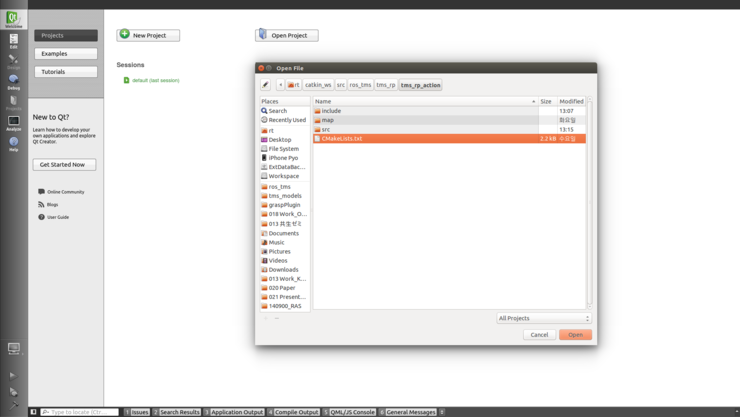
\includegraphics[width=0.9\columnwidth]{pictures/chapter2/qtcreator2.png}
\caption{QtCreator: 프로젝트 열기}
\end{figure}

\begin{figure}[h]
\centering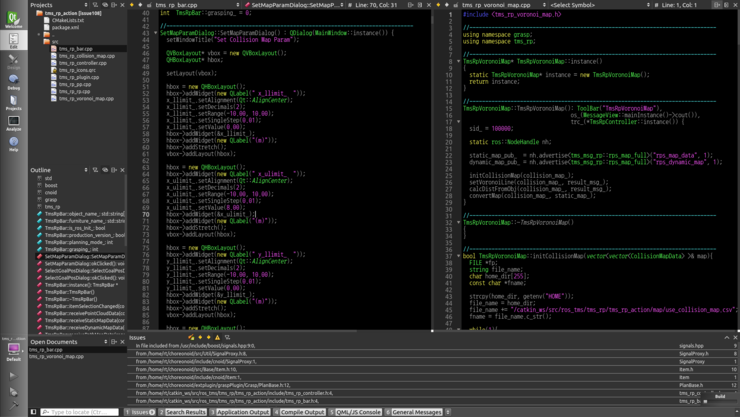
\includegraphics[width=0.9\columnwidth]{pictures/chapter2/qtcreator3.png}
\caption{QtCreator: 프로젝트 전개 모습}
\end{figure}

%-------------------------------------------------------------------------------
\section{ROS 동작 테스트}\index{ROS 동작 테스트}

%-------------------------------------------------------------------------------
\subsection{turtlesim 패키지}
일단, ROS를 설치하긴 했는데, 제대로 작동되는지 궁금하신분들을 위해 ROS에서 제공하는 간단한 예제 노드를 실행하는 방법에 대해 설명한다. 예제는 turtlesim 이라는 패캐지(노드의 묶음)로 ROS의 심볼인 거북이 모양을 한 로봇이 화면에 나타나고 키보드로 로봇의 이동을 간단히 조종해 보는 노드(프로그램)이다.

이번 내용부터는 노드(Node), 패키지(package), roscore 등 ROS 의 고유의 용어들이 많이 등장하는데 이번 강좌에서는 단순히 이런게 있구나 알아두기 바라며, 자세한 설명은 \textbf{섹션~\ref{sec:RosTerm}~\nameref{sec:RosTerm}(pp.\pageref{sec:RosTerm})} 에서 설명하도록 하겠다. 이번 강좌는 ROS 가 문제없이 설치됨을 확인정도 이기 때문에 본격적인 ROS 강좌가 들어가기 전에 몸풀기 운동 정도로 생각하자.

%-------------------------------------------------------------------------------
\subsection{roscore 실행}
새로운 터미널을 열어 다음과 같은 명렁어를 실행한다. 그러면 모든 ROS 시스템을 관할하는 roscore가 실행되게 된다.
\\
\begin{lstlisting}[language=ROS]
$ roscore
\end{lstlisting}

\begin{figure}[h]
\centering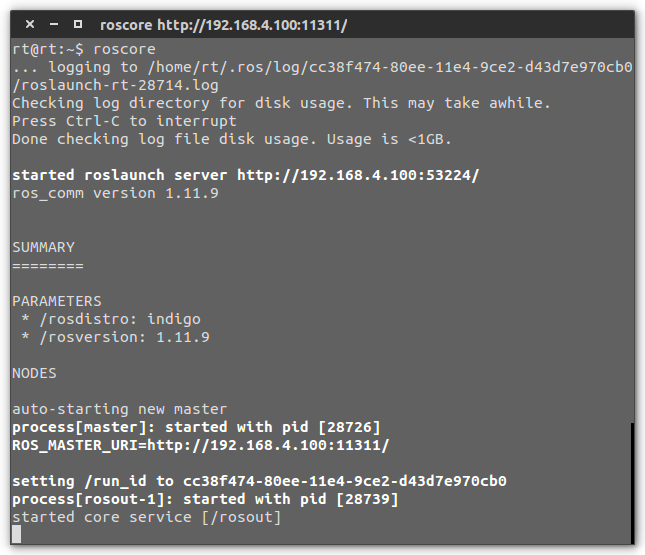
\includegraphics[width=0.7\columnwidth]{pictures/chapter2/roscore.png}
\caption{roscore가 실행된 화면}
\end{figure}

%-------------------------------------------------------------------------------
\subsection{turtlesim 패키지의 turtlesim\_node 실행}
새로운 터미널을 열어 다음과 같은 명렁어를 실행한다. 그러면 다음와 같은 메시지를 보게 되며, turtlesim 패키지의 turtlesim\_node 를 실행하게 된다. 별도의 창에 파란색 바탕의 화면에 거북이 한 마리가 보일 것이다. (거북이 모양은 실행에 따라 랜덤으로 바뀌기 때문에 필자의 모양과는 다를 수 있다.)
\\
\begin{lstlisting}[language=ROS]
$ rosrun turtlesim turtlesim_node
[ INFO] [1418273733.244561023]: Starting turtlesim with node name /turtlesim
[ INFO] [1418273733.249333831]: Spawning turtle [turtle1] at x=[5.544445], y=[5.544445], theta=[0.000000]
\end{lstlisting}

\begin{figure}[h]
\centering
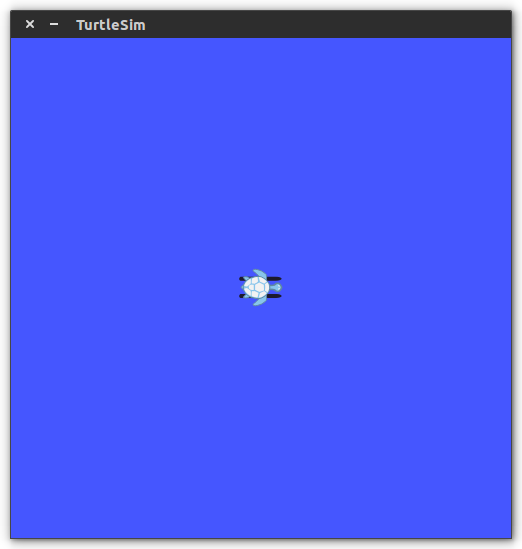
\includegraphics[width=0.49\columnwidth]{pictures/chapter2/turtlesim_node.png}
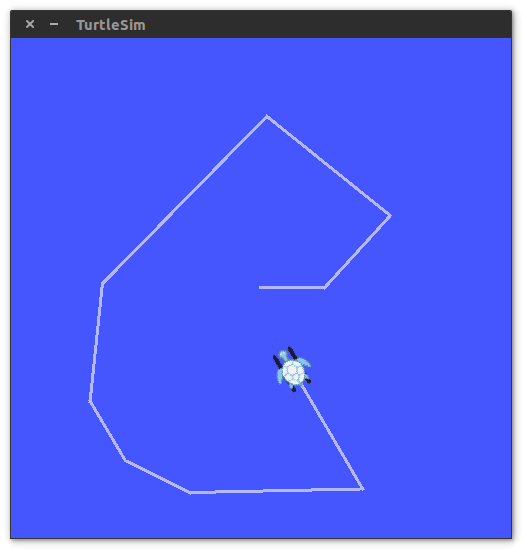
\includegraphics[width=0.49\columnwidth]{pictures/chapter2/turtlesim_node_move.png}
\caption{turtlesim\_node 노드를 실행하고 turtle\_teleop\_key 노드를 실행하여 화면위의 거북이를 이동시킨 모습}
\label{fig:turtlesim_node}
\end{figure}

%-------------------------------------------------------------------------------
\subsection{turtlesim 패키지의 turtle\_teleop\_key 실행}
새로운 터미널을 열어 다음과 같은 명렁어를 실행한다. 그러면 다음과 같은 메시지를 보게 되며, turtlesim 패키지의 turtle\_teleop\_key를 실행하게 된다. 이 \textbf{터미널 창 위}에서 키보드의 화살표(← → ↑ ↓)를 이용하여 그림\ref{fig:turtlesim_node}의 우측과 같이 거북이를 제어하게 된다. 간단하므로 직접 해보길 바란다. 제어하게 되면 화면 속의 거북이가 움직이게 되는데, 이는 간단히 시뮬레이션이지만 실제 로봇도 이와 같은 방법으로 원격조정이 가능하게 된다.
\\
\begin{lstlisting}[language=ROS]
$ rosrun turtlesim turtle_teleop_key
Reading from keyboard
---------------------------
Use arrow keys to move the turtle.
\end{lstlisting}

%-------------------------------------------------------------------------------
\subsection{rqt\_graph 패키지의 rqt\_graph 실행}
새로운 터미널을 열어 다음와 같은 명렁어를 실행한다. 그러면 rqt\_graph 패키지의 rqt\_graph 노드가 실행되게 된다. 그 결과 그림\ref{fig:turtlesim_node_graph} 같은 그래프를 볼 수 있을 것이다. 이는 현재 실행중인 노드(프로그램)들의 정보를 그래프로 볼 수 있는 노드이다.
\\
\begin{lstlisting}[language=ROS]
$ rosrun rqt_graph rqt_graph
\end{lstlisting}

rqt\_graph 노드는 현재 실행 중인 노드들의 정보를 볼 수 있는 GUI 형태의 노드이다. 동그라미는 노드를 의미하고, 네모는 토픽을 의미한다. 다음의 그림을 자세히 보자. /teleop\_turtle 노드로부터 화살표가 그어져 /turtlesim 으로 이어져 있다. 이는 두 노드가 실행 중 이고, 이 두 노드 간에는 메시지 통신이 이루어 지고 있다는 설명이다. 

그리고 화살표 사이의 네모박스 turtle1 토픽의 하위 토픽인 /turtle1/cmd\_vel 는 두 노드간의 토픽의 이름으로, teleop\_turtle 노드에서 키보드로 입력한 속도 명령이 turtlesim 으로 토픽을 통해 메세지(msg 데이타)가 송신되고 있다는 내용이다. 

즉, 위에서 실행한 두 노드를 이용하여 키보드 명령을 로봇 시뮬레이션에게 전달해 줬다는 내용이다. 자세한 내용은 추후 이어지는 내용에서 하도록 하고, 여기까지 진행이 원만히 되었다면, ROS 구동 테스트는 끝나게 된다.

\begin{figure}[h]
\centering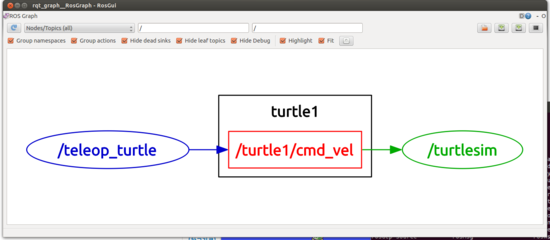
\includegraphics[width=0.8\columnwidth]{pictures/chapter2/turtlesim_node_graph.png}
\caption{노드들의 정보를 볼 수 있는 GUI 형태의 rqt\_graph 노드}
\label{fig:turtlesim_node_graph}
\end{figure}

%-------------------------------------------------------------------------------
\subsection{노드의 종료}

각각 실행된 roscore 및 노드는 터미널 창에서 Ctrl + c 를 눌러 종료한다.

%-------------------------------------------------------------------------------

% \chapterimage{chapter_head_1.pdf} % Chapter heading image

% \chapter{Presenting Information}

% \section{Table}\index{Table}

% \begin{table}[h]
% \centering
% \begin{tabular}{l l l}
% \toprule
% \textbf{Treatments} & \textbf{Response 1} & \textbf{Response 2}\\
% \midrule
% Treatment 1 & 0.0003262 & 0.562 \\
% Treatment 2 & 0.0015681 & 0.910 \\
% Treatment 3 & 0.0009271 & 0.296 \\
% \bottomrule
% \end{tabular}
% \caption{Table caption}
% \end{table}

% %-------------------------------------------------------------------------------

% \section{Figure}\index{Figure}

% \begin{figure}[h]
% \centering
\includegraphics[scale=0.5]{placeholder}
% \caption{Figure caption}
% \end{figure}
% -*- root: main.tex -*-
%-------------------------------------------------------------------------------
\chapterimage{chapter_head_4.pdf} 

%-------------------------------------------------------------------------------
\chapter{ROS 개념 정리}

%-------------------------------------------------------------------------------
\section{ROS 용어 정리}\index{ROS 용어 정리}\label{sec:RosTerm}

ROS는 수 없이 많은 독특한 용어들이 사용된다. 여기에 많이 등장하는 ROS 용어들을 골라 정리하였다. ROS 용어 사전처럼 이용하면 좋을 듯 싶다. 대부분이 처음보는 용어일 수 있다. 이해가 안된다고 포기하지 말고 이해 안되는 부분은 일단 접어두고 내용으로 넘어가서 직접 실전을 통해 익힐 수 있도록 하자.

\vspace{\baselineskip}
\begin{definition}[ROS]\label{def:Ros}
ROS는 로봇 응용 프로그램을 개발을 위한 운영 체제와 같은 로봇 플랫폼이다. ROS는 로봇 응용프로그램을 개발할 때 필요한 하드웨어 추상화, 하위 디바이스 제어, 일반적으로 사용되는 기능의 구현, 프로세스간의 메시지 파싱, 패키지 관리, 개발환경에 필요한 라이브러리와 다양한 개발 및 디버깅 도구를 제공한다.
\end{definition}

\vspace{\baselineskip}
\begin{definition}[마스터(master)]\label{def:RosMaster}
마스터는 노드와 노드사이의 연결 및 메시지 통신을 위한 네임 서버와 같은 역할을 한다. roscore가 실행 명령어 이며, 마스터를 실행하면 각 노드들의 이름을 등록하고 필요에 따라 정보를 받을 수 있다. 마스터가 없이는 노드간의 접속, 토픽과 서비스와 같은 메시지 통신을 할 수 없다. 

마스터는 마스터에 접속하는 슬레이브들과의 접속 상태를 유지하지 않는 HTTP 기반의 프로토콜인 XMLRPC를 이용하여 슬레이브들과 통신하게 된다. 즉, 슬레이브인 노드들이 필요할때만 접속하여 자신의 정보를 등록하거나 다른 노드의 정보를 요청하여 수신받을 수 있다. 평상시에는 서로간의 접속 상태를 체크하지 않는다. 이러한 기능으로 매우 크고, 복잡한 환경에서도 적용 가능하다. 또한, XMLRPC는 매우 가볍고, 다양한 프로그래밍 언어를 지원하고 있기 때문에 다기종 하드웨어, 다언어를 지원하는 ROS에 매우 적합하다.

ROS를 구동하게 되면 사용자가 정해놓은 ROS\_MASTER\_URI 변수에 기재되어 있는 URI 주소 및 포트를 갖는다. 사용자가 설정해놓지 않은 경우에는 URI 주소로 현재의 로컬 IP 를 사용하고, 11311 포트를 이용하게 된다.
\end{definition}

\vspace{\baselineskip}
\begin{definition}[노드(node)]\label{def:RosNode}
ROS에서 최소 단위의 실행 프로세서를 가르키는 용어이다. 하나의 실행 가능한 프로그램으로 생각하면 된다. ROS에서는 하나의 목적에 하나의 노드를 작성하길 권하고 있으며 재사용이 쉽도록 구성하여 만들도록 권고하고 있다. 예를들어, 모바일 로봇의 경우, 로봇을 구동하기 위하여 각 프로그램을 세분화 시킨다. 예를들어, 센서 드라이브, 센서 데이타를 이용한 변환, 장애물 판단, 모터 구동, 엔코더 입력, 네이게이션 등 세부화된 작은 노드들을 이용한다.

노드는 생성과 함께 마스터에 노드이름, 발행자이름, 구독자이름, 토픽이름, 서비스이름, 메시지형태, URI 주소 및 포트를 등록한다. 이 정보들을 기반으로 각 노드는 노드끼리 토픽 및 서비스를 이용하여 메시지를 주고 받을 수 있다.

노드는 마스터와 통신할 때, XMLRPC를 이용하며, 노드간의 통신에서는 XMLRPC 및 TCP/IP 통신 계열의 TCPROS를 이용하고 있다. 노드간의 접속 요청 및 응답은  XMLRPC를 사용하며, 메시지 통신은 마스터와는 관계없이 노드와 노드간의 직접적인 통신으로 TCPROS를 이용하고 있다. URI 주소 및 포트는 현재 노드가 실행중인 컴퓨터에 저장된 ROS\_HOSTNAME 라는 환경 변수값을 URI 주소로 사용하며, 포트는 임의적 고유의 값으로 설정되게 된다.  
\end{definition}

\vspace{\baselineskip}
\begin{definition}[패키지(package)]\label{def:RosPackage}
ROS를 구성하는 기본 단위로써 실행 가능한 노드를 포함하고 있다. ROS는 패키지를 단위로 각각의 응용 프로그램들이 개발된다. 패키지는 최소한 하나 이상의 노드를 포함하고 있다. ROS Indio의 경우 공식적으로 약 970개 의 패키지를 제공하고 있으며, 유저들이 개발하여 공개된 패키지가 대략 3300개에 달하고 있다. 
\end{definition}

\vspace{\baselineskip}
\begin{definition}[메타패키지(metapackage)]\label{def:RosMetapackage}
공통된 목적을 가지는 패키지들을 모아둔 패키지들의 집합을 말한다. 복수의 패키지를 포함하고 있다.
\end{definition}

\vspace{\baselineskip}
\begin{definition}[메시지(message,msg)]\label{def:RosMessage}
노드는 메시지를 통해 노드간의 데이터를 주고받게 된다. 메시지는 integer, floating point, boolean 와 같은 변수 형태이다. 또한, 메시지안에 메시지를 품고 있는 간단한 데이터 구조 및 메시지들의 배열과 같은 구조도 사용할 수 있다. 

메세지를 이용한 통신방법으로는 TCPROS, UDPROS 방식등이 있으며, 단방향 메시지 송/수신 방식의 토픽과 양방향 메시지 요청/응답 방식의 서비스를 이용하고 있다.
\end{definition}

\vspace{\baselineskip}
\begin{definition}[토픽(topic)]\label{def:RosTopic}
토픽은 "이야깃거리"이다. 발행자 노드가 하나의 이야깃거리에서 대해서 토픽이라는 이름으로 마스터에 등록한 후, 이야깃거리에 대한 이야기를 메시지 형태로 발행한다. 이 이야깃거리를 수신 받기를 원하는 구독자 노드는 마스터에 등록된 토픽의 이름에 해당되는 발행자 노드의 정보를 받는다. 이 정보를 기반으로 구독자 노드는 발행자 노드와 직접적으로 연결하여 메시지를 송/수신 또는 요청/응답 받게 된다. 
\end{definition}

\vspace{\baselineskip}
\begin{definition}[발행(publish) 및 발행자(Publisher) ]\label{def:RosPublish}
발행은 토픽의 내용에 해당되는 메시지 형태의 데이터를 송신하는 것을 말한다. 발행자 노드는 발행을 수행하기 위하여 토픽을 포함한 자신의 정보들을 마스터에 등록하고, 구독을 원하는 구독자 노드에게 메시지를 보내게 된다. 발행자는 이를 실행하는 개체로써 노드에서 선언하게 된다. 발행자는 하나의 노드에서 복수로 선언이 가능하다.
\end{definition}

\vspace{\baselineskip}
\begin{definition}[구독(subscribe) 및 구독자(Subscriber)]\label{def:RosSubscribe}
구독은 토픽의 내용에 해당되는 메시지 형태의 데이터를 수신하는 것을 말한다. 구독자 노드는 구독을 수행하기 위하여 토픽을 포함한 자신의 정보들을 마스터에 등록하고, 구독하고자 하는 토픽을 발행하는 발행자 노드의 정보를 마스터로부터 받는다. 이 정보를 기반으로 구독자 노드는 발행자 노드와 직접적으로 접속하여 발행자 노드로부터 메시지를 받게 된다. 구독자는 이를 실행하는 개체로써 노드에서 선언하게 된다. 구독자는 하나의 노드에서 복수로 선언이 가능하다.
\end{definition}

\vspace{\baselineskip}
\begin{definition}[서비스(service)]\label{def:RosService}
발행과 구독 개념의 토픽 통신 방식은 비동기 방식이라 필요에 따라서 주어진 데이터를 전송하고 받기에 매우 훌륭한 방법이다. 또한, 한번의 접속으로 지속적인 메시지를 송/수신하기 때문에 지속적으로 메시지를 발송해야하는 센서 데이터에 적합하여 많이 사용되고 있다. 하지만, 경우에 따라서는 요청과 응답이 함께 사용되는 동기 방식의 메시지 교환 방식도 필요하다. 이에 따라, ROS에서는 서비스라는 이름으로 메시지 동기 방식을 제공하고 있다. 서비스는 요청이 있을 경우에 응답을 하는 서비스 서버와 요청을 하고 응답을 받는 서비스 클라이언트로 나뉘어 있다. 서비스는 토픽과는 달리 1회성 메시지 통신이다. 서비스의 요청과 응답이 완료되면 연결된 두 노드의 접속은 끊기게 된다. 
\end{definition}

\vspace{\baselineskip}
\begin{definition}[서비스 서버 (service server)]\label{def:RosServiceServer}
서비스 서버는 요청을 입력으로 받고, 응답을 출력으로 하는 서비스 메시지 통신의 서버 역할을 말한다. 요청과 응답은 모두 메시지로 되어 있으며, 서비스 요청에 의하여 주어진 서비스를 수행 후에 그 결과를 서비스 클라이언트에게 전달한다. 서비스 메시지 방식은 동기식이기에 정해진 명령을 지시 및 수행하는 노드에 사용하는 경우가 많다.
\end{definition}

\vspace{\baselineskip}
\begin{definition}[서비스 클라이언트 (service client)]\label{def:RosServiceClient}
서비스 클라이언트는 요청을 출력으로 하고, 응답을 입력으로 받는 서비스 메시지 통신의 클라이언트 역할을 말한다. 요청과 응답은 모두 메시지로 되어 있으며, 서비스 요청을 서비스 서버에 전달하고 그 결과 값을 서비스 서버로 부터 받는다. 서비스 메시지 방식은 동기식이기에 정해진 명령을 지시 및 수행하는 노드에 사용하는 경우가 많다.
\end{definition}

\vspace{\baselineskip}
\begin{definition}[캐킨(catkin)]\label{def:RosCatkin}
ROS의 빌드 시스템을 말한다. ROS의 빌드 시스템은 기본적으로 CMake(Cross Platform Make) 를 이용하고 있어서 패키지 폴더에 CMakeLists.txt 라는 파일에 빌드 환경을 기술하고 있다. ROS에서는 CMake 를 ROS에 맞도록 수정하여 ROS에 특화된 캐킨 빌드 시스템을 만들었다. 캐킨 빌드 시스템은 ROS와 관련된 빌드, 패키지 관리, 패키지간의 의존관계 등을 편리하게 사용할 수 있도록 하고 있다. 
\end{definition}

\vspace{\baselineskip}
\begin{definition}[ROS빌드(rosbuild)]\label{def:RosRosbuild}
catkin 빌드 시스템의 이전에 사용되었던 빌드 시스템이다. ROS Fuerte 버전부터 rosbuild 빌드 시스템 대신에 catkin 빌드 시스템을 사용하고 있으나, rosbuild 빌드 시스템 또한 사용 가능하다. 하지만, 이는 ROS 버전의 호환성을 위해 남겨둔 것이지 공식적으로는 추천하지 않는다. 만약, rosbuild 빌드 시스템을 사용한 이전 패키지를 사용해야만 한다면 rosbuild를 catkin으로 변경하여 사용하기를 추천한다. 
\end{definition}

\vspace{\baselineskip}
\begin{definition}[ROS코어(roscore)]\label{def:RosCore}
ROS 마스터를 구동하는 명령어이다. 같은 네트웍이라면 다른 컴퓨터에서 실행하여도 된다. 단, 멀티 ROS코어를 지원하는 특수한 경우를 제외하고는 ROS코어는 동일 네트워크에서 하나만 구동되게 디노다. ROS를 구동하게 되면 사용자가 정해놓은 ROS\_MASTER\_URI 변수에 기재되어 있는 URI 주소 및 포트를 갖는다. 사용자가 설정해놓지 않은 경우에는 URI 주소로 현재의 로컬 IP 를 사용하고, 11311 포트를 이용하게 된다.
\end{definition}

\vspace{\baselineskip}
\begin{definition}[매개변수(parameter)]\label{def:RosParameter}
노드에서 사용되는 매개변수를 말한다. 흔히, 윈도우즈 프로그램에서 *.ini 설정파일과 같다고 생각하면 된다. 디폴트로 설정 값들이 지정되어 있고, 필요에 의해서 외부에서 이 매개변수를 읽기, 쓰기가 가능하다. 특히, 상황에 맞추어 이 매개변수를 외부에서 쓰기기능을 이용하여 설정값을 실시간으로 바꿀수 있기에 매우 유용한 방법이다. 예를들어 접속하는 USB포트 및 카메라 캘리브레이션 값, 속도 및 명령어들의 최대/최저 값 등의 설정등을 지정할 수 있다.
\end{definition}

\vspace{\baselineskip}
\begin{definition}[매개변수 서버(parameter server)]\label{def:RosParameterServer}
매개변수 서버는 패키지에서 매개변수를 사용할 때, 각 매개변수를 등록하는 서버를 말한다. 매개변수 서버는 마스터의 일부분이다. 
\end{definition}

\vspace{\baselineskip}
\begin{definition}[rosrun]\label{def:RosRun}
ROS의 기본적인 실행 명령어이다. 패키지에서 하나의 노드를 실행하는데 사용된다. 노드가 사용하는 URI 주소 및 포트는 현재 노드가 실행중인 컴퓨터에 저장된 ROS\_HOSTNAME 라는 환경 변수값을 URI 주소로 사용하며, 포트는 임의적 고유의 값으로 설정되게 된다.
\end{definition}

\vspace{\baselineskip}
\begin{definition}[roslaunch]\label{def:RosLaunch}
rosrun이 하나의 노드를 실행하는 명령어라면 ROS런치(roslaunch)는 복 수개의 노드를 실행하는 개념이다. 이 명령어를 통해 정해진 단일 혹은 복수의 노드를 실행시킬 수 있다. 

그 이외의 기능으로 실행시에 패키지의 매개변수를 변경, 노드 명의 변경, 노드 네임 스페이스 설정, ROS\_ROOT 및 ROS\_PACKAGE\_PATH 설정, 이름 변경, 환경 변수 변경 등의 실행시 변경할 수 있는 많은 옵션들을 갖춘 노드 실행에 특화된 ROS 명령어이다. 

ROS런치는 *.launch 라는 ROS런치파일을 사용하여 실행 노드에 대한 설정을 해주는데 이는 XML 기반으로 되어 있으며, 태그별 옵션을 제공하고 있다.
\end{definition}

\vspace{\baselineskip}
\begin{definition}[배그(bag)]\label{def:RosBag}
ROS에서 주고받는 메시지의 데이터를 저장할 수 있는 있는데 이를 배그라고 한다. ROS에서는 이 배그를 이용하여 메시지를 저장하고 필요로 할 때 이를 재생하여 이전 상황을 그대로 재현할 수있는 기능을 갖추고 있다. 예를들어, 센서를 이용한 로봇 실험을 실행할 때, 센서 값을 배그를 이용하여 메시지 형태로 저장한다. 이 저장된 메시지는 같은 실험을 수행하지 않아도 저장해둔 배그 파일을 재생하는 것으로 그 당시의 센서값을 반복 사용가능하다. 특히, 기록, 재생의 기능을 활용하여 반복되는 프로그램 수정이 많은 알고리즘 개발에 매우 유용하다. 
\end{definition}

\vspace{\baselineskip}
\begin{definition}[ROS Wiki]\label{def:RosWiki}
ROS의 각 패키지 및 기능들을 설명하는 페이지(\url{http://wiki.ros.org/})이다. 각 패키지는 위키 페이지에 패키지에 대한 간단한 설명, 사용되는 매개변수, 저작자, 라이선스, 홈페이지, 저장소, 튜토리얼등을 기술하고 있다.
\end{definition}

\vspace{\baselineskip}
\begin{definition}[저장소(repositoy)]\label{def:RosRepository}
공개된 패키지의 경우, 각 패키지의 위키에 저장소를 명시하고 있다. 저장소는 패키지가 저장된 웹상의 저장소 URL 주소이며 svn, hg, git 등의 소스 관리 시스템을 이용하여 이슈, 개발, 다운로드 등을 관리하고 있다.
\end{definition}

\vspace{\baselineskip}
\begin{definition}[그래프(graph)]\label{def:RosGraph}
위에서 설명한 노드, 토픽, 발행자, 구독자 관계를 그래프를 통해 나타나게 하는 것이다. 현재 실행중인 메시지 통신을 그래프화 시킨 것으로 1회성 서비스에 대한 그래프는 작성할 수 없다. 실행은 rqt\_graph 패키지의 rqt\_graph 노드를 실행하면 된다. 실행 명령에는 두 가지가 있는데 rqt\_graph과 rosrun rqt\_graph rqt\_graph 이다.   
\end{definition}

\vspace{\baselineskip}
\begin{definition}[이름(name)]\label{def:RosName}
노드, 매개변수, 토픽, 서비스는 모두 이름을 갖고 있다. 이 이름은 마스터에 등록하고 각 노드의 매개변수, 토픽, 서비스를 사용할때 이 이름을 기반으로 상호적으로 동작하도록 되어있다. 또한, 이름은 실행시에 변경가능하기 때문에 매우 유연하고, 같은 노드, 매개변수, 토픽, 서비스라고 하여도 다른 이름으로 중복 실행이 가능하다. 이러한 이름의 사용으로 ROS는 큰 규모의 프로젝트, 복잡한 구조의 시스템에도 적합하다.  
\end{definition}

\vspace{\baselineskip}
\begin{definition}[클라이언트 라이브러리(client libray)]\label{def:RosClientLibray}
ROS는 사용되는 언어의 의존성을 낮추기 위하여 클라이언트 라이브러리라는 이름으로 각종 언어의 개발환경을 제공하고 있다. 주요한 클라이언트 라이브러리로는 C++, Python, Lisp 등이 있으며, 그 이외에도 java, lua, .NET, EusLisp, R 등의 언어들을 사용가능하다. 이를 위해 roscpp, rospy, roslisp, rosjava, roslua, roscs, roseus, PhaROS, rosR 등의 클라이언트 라이브러리가 개발되었다.
\end{definition}

\vspace{\baselineskip}
\begin{definition}[URI (Uniform Resource Identifier)]\label{def:RosURI}
URI (Uniform Resource Identifier, 통합 자원 식별자) 는 인터넷에 있는 자원을 나타내는 유일한 주소이다. URI 은 인터넷에서 요구되는 기본조건으로서 인터넷 프로토콜에서 식별자로 사용된다.
\end{definition}

\vspace{\baselineskip}
\begin{definition}[MD5 (Message-Digest algorithm 5)]\label{def:RosMD5}
MD5는 128비트 암호화 해시 함수이다. 주로 프로그램이나 파일이 원본 그대로인지를 확인하는 무결성 검사 등에 사용된다. ROS에서의 메시지를 이용한 통신에서 MD5를 이용하여 메시지 송수신의 무결성 검사를 하고 있다.
\end{definition}

\vspace{\baselineskip}
\begin{definition}[RPC(Remote Procedure Call)]\label{def:RosRPC}
RPC란 '멀리 떨어져(Remote) 있는 컴퓨터상의 프로그램이 다른 컴퓨터 내에 있는 서브프로그램(Procedure)을 불러내는(Call)' 것을 의미한다. 컴퓨터 프로그램이 다른 주소 공간에서 원격 제어를 위한 프로그래머의 세세한 코딩 없이 함수나 프로시저의 실행을 허용하는 기술로써 대표적으로는 TCP/IP, IPX 등의 전송 프로토콜을 이용한다. 
\end{definition}

\vspace{\baselineskip}
\begin{definition}[XML(Extensible Markup Language)]\label{def:RosXML}
XML은 W3C에서 다른 특수 목적의 마크업 언어를 만드는 용도에서 권장되는 다목적 마크업 언어(markup language)로 태그 등을 이용하여 데이터의 구조를 명기하는 언어의 한 가지이다. 
\end{definition}

\vspace{\baselineskip}
\begin{definition}[XMLRPC]\label{def:RosXMLRPC}
XML-RPC란, RPC 프로토콜의 일종으로서, 인코딩 형식에서는 XML을 채택하고, 전송 방식에서는 접속 상태를 유지하지 않고 체크하지 않는 요청/응답 방식의 HTTP 프로토콜을 사용하고 있다. XML-RPC는 매우 단순한 규약으로서, 작은 데이터 형식이나 명령을 정의하는 정도로만 사용하고 있어서 꽤나 단순한 편이다. 이러한 특징으로, XMLRPC는 매우 가볍고, 다양한 프로그래밍 언어를 지원하고 있기 때문에 다기종 하드웨어, 다언어를 지원하는 ROS에 매우 적합하다.
\end{definition}

\vspace{\baselineskip}
\begin{definition}[TCP/IP (Transmission Control Protocol / Internet Protocol)]\label{def:RosTCPIP}
TCP 는 Transmission Control Protocol 의 약자로써, 전송 제어 프로토콜이라고 부른다. 흔히 TCP/IP 라 부르는데 이는 인터넷 프로토콜 계층의 시각에서 보면 IP(Internet Protocol) 를 기반으로 전송 제어 프로토콜인 TCP 를 사용하여 데이터의 전달을 보증하고 보낸 순서대로 송/수신하게 된다. 
\end{definition}

\vspace{\baselineskip}
\begin{definition}[TCPROS]\label{def:RosTCPROS}
메시지 및 서비스에서 사용되는 TCP/IP 기반의 메시지 방식을 TCPROS라고 한다.
\end{definition}

\vspace{\baselineskip}
\begin{definition}[UDPROS]\label{def:RosUDPROS}
메시지 및 서비스에서 사용되는 UDP 기반의 메시지 방식을 UDPROS라고 한다. 일반적으로 ROS에서는 사용되지 않고 있다.
\end{definition}

\vspace{\baselineskip}
\begin{definition}[CMakeLists.txt]\label{def:RosCMakeLists.txt}
ROS의 빌드 시스템인 캐킨은 기본적으로 CMake를 이용하고 있어서 패키지 폴더에 CMakeLists.txt 라는 파일에 빌드 환경을 기술하고 있다.
\end{definition}

\vspace{\baselineskip}
\begin{definition}[package.xml]\label{def:RosPackage.XML}
패키지의 정보를 담은 XML 파일로써 패키지의 이름, 저작자, 라이선스, 의존성 패키지 등을 기술하고 있다.
\end{definition}

\newpage
%-------------------------------------------------------------------------------
\section{ROS 개념 정리}\index{ROS 개념 정리}

%-------------------------------------------------------------------------------
\subsection{메시지 통신}\index{메시지 통신}

지금까지 ROS에 대해서 설명하였지만, 실제로 어떻게 동작하는 것인지에 대해서는 자세히 언급하지 않았었다. 이번 강좌에서는 ROS의 동작에 대한 핵심 기능 및 개념에 대해서 설명하려고 한다. ROS는 매우 생소한 용어들이 많이 등장하므로 \textbf{섹션~\ref{sec:RosTerm}~\nameref{sec:RosTerm}(pp.\pageref{sec:RosTerm})}를 참고하면서 ROS 개념을 이해하면 좋을 듯 싶다. ROS 개념 설명에서 사용되는 각 용어들의 상세한 설명은 용어 정리 강좌를 참조하기 바라며, 이번 강좌에서는 개념만을 설명하도록 하겠다.

ROS의 핵심 개념은 노드간의 메시지 통신\footnote{ROS Wiki, Concepts, \url{http://wiki.ros.org/ROS/Concepts}}\footnote{ROS Wiki, Higher-Level Concepts, \url{http://wiki.ros.org/ROS/Higher-Level\%20Concepts}}이다. 목적에 따라 세분화된 최소 단위의 실행 프로그램인 노드는 다른 노드와 처리 결과 값을 주고 받게 됨으로써 하나의 커다란 프로그램이 된다. 이를 위하여 메시지 통신에는 단 방향으로 연속적으로 메시지를 송수신하는 토픽 메시지 통신과 쌍 방향으로 요청과 응답 형태의 정해진 작업을 수행하게 하는 목적의 서비스 메시지 통신이 있다. 

이러한 노드간의 메시지 통신에는 접속이 필요한데, 노드간의 접속을 돕는 것이 마스터\footnote{ROS Wiki, Master, \url{http://wiki.ros.org/Master}}이다. 마스터는 노드의 이름, 토픽 및 서비스의 이름, URI 주소와 포트, 매개변수 등의 네임 서버와 같은 역할을 하게된다. 즉, 노드는 생성과 동시에 마스터에 자신의 정보를 등록하게 되고, 다른 노드가 마스터를 통해 접속하려는 노드의 정보를 마스터로부터 취득한다. 그 후, 노드와 노드가 직접 접속하여 메시지 통신을 하는 것이다. 

이를 그림으로 나태내면 다음의 그림과 같다. 마스터는 노드들의 정보를 관리하며, 각 노드는 필요에 따라 다른 노드와 접속, 메시지 통신을 하게 된다. 여기서 우리는 가장 중요한 마스터, 노드, 토픽\footnote{ROS Wiki, Topics, \url{http://wiki.ros.org/Topics}}, 서비스\footnote{ROS Wiki, Services, \url{http://wiki.ros.org/Services}}, 메시지\footnote{ROS Wiki, Messages, \url{http://wiki.ros.org/Messages}}의 흐름에 대해서 알아보도록 하자.

\begin{figure}[h]
\centering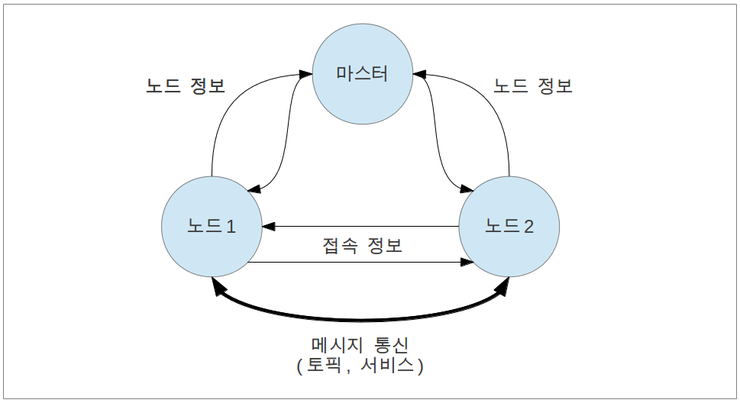
\includegraphics[width=\columnwidth]{pictures/chapter4/message_communication.png}
\caption{메시지 통신}
\end{figure}


%-------------------------------------------------------------------------------
\subsection{마스터 구동}\index{마스터 구동}

노드들간의 메시지 통신에서 연결 정보를 관리하는 마스터는 ROS를 사용하기 위해서 제일 먼저 구동해야하는 필수 요소이다. 다음과 같이 roscore라는 실행 명령어로 ROS 마스터는 구동되며, XMLRPC으로 서버를 구동하게 된다. 마스터는 노드간의 접속을 위하여 노드들의 이름, 토픽 및 서비스의 이름, 메시지 형태, URI 주소 및 포트를  등록받고, 요청이 있을 경우 이 정보를 다른 노드에게 알려주는 역할을 한다.

\begin{lstlisting}[language=ROS]
$ roscore
\end{lstlisting}

\begin{figure}[h]
\centering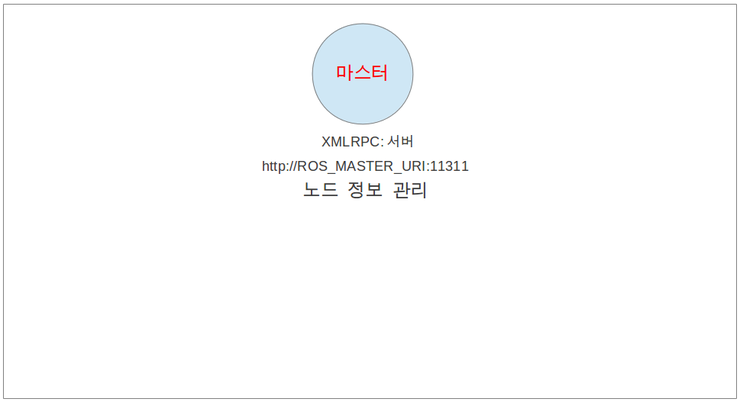
\includegraphics[width=0.7\columnwidth]{pictures/chapter4/notion1.png}
\caption{마스터 구동}
\end{figure}

%-------------------------------------------------------------------------------
\subsection{구독자 노드(Node) 구동}\index{구독자 노드(Node) 구동}
 
구독자 노드는 다음과 같이 rosrun 및 roslaunch 이라는 실행 명령어로 구동된다. 구독자 노드는 구동과 함께 마스터에 자신의 구독자노드이름, 토픽이름, 메시지형태, URI 주소 및 포트를 등록한다. 마스터와 노드는 XMLRPC 를 이용하여 통신하게 된다.

\begin{lstlisting}[language=ROS]
$ rosrun PACKAGE_NAME NODE_NAME
$ roslaunch PACKAGE_NAME LAUNCH_NAME
\end{lstlisting}

\begin{figure}[h]
\centering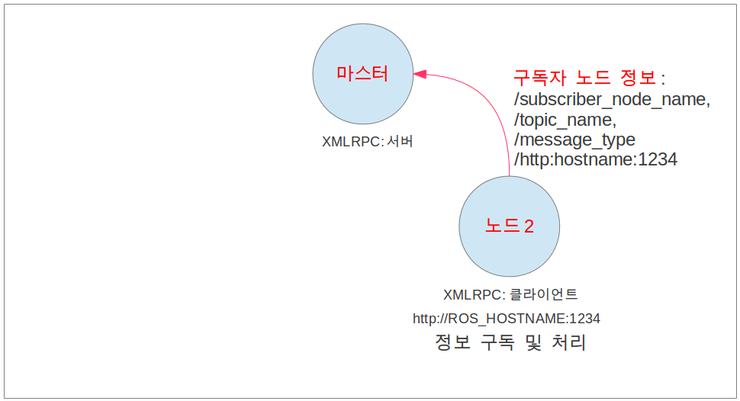
\includegraphics[width=0.7\columnwidth]{pictures/chapter4/notion2.png}
\caption{구독자 노드 구동}
\end{figure}

\newpage
%-------------------------------------------------------------------------------
\subsection{발행자 노드(Node) 구동}\index{발행자 노드(Node) 구동}

발행자 노드는 구독자 노드와 마찬가지로 rosrun 및 roslaunch 이라는 실행 명령어로 구동한다. 발행자 노드는 구동과 함께 마스터에 자신의 발행자노드이름, 토픽이름, 메시지형태, URI 주소 및 포트를 등록한다. 마스터와 노드는 XMLRPC 를 이용하여 통신하게 된다.

\begin{figure}[h]
\centering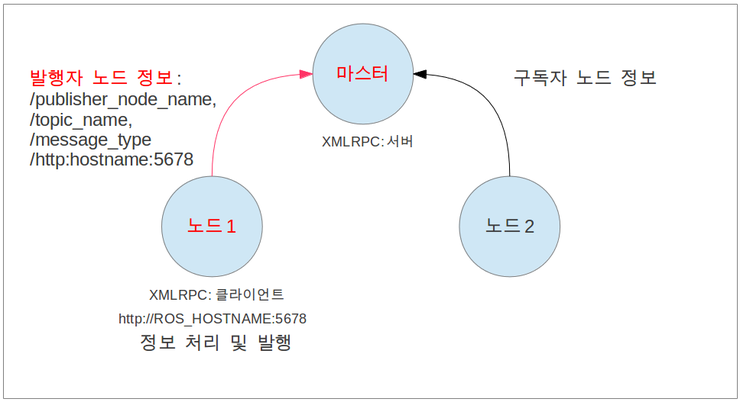
\includegraphics[width=0.9\columnwidth]{pictures/chapter4/notion3.png}
\caption{발행자 노드 구동}
\end{figure}

%-------------------------------------------------------------------------------
\subsection{발행자 정보 알림}\index{발행자 정보 알림}

마스터는 구독자 노드에게 접속하기 원하는 발행자의 이름, 주소등의 정보를 접속하고자하는 노드에게 알린다. 마스터와 노드는 XMLRPC 를 이용하여 통신하게 된다.

\begin{figure}[h]
\centering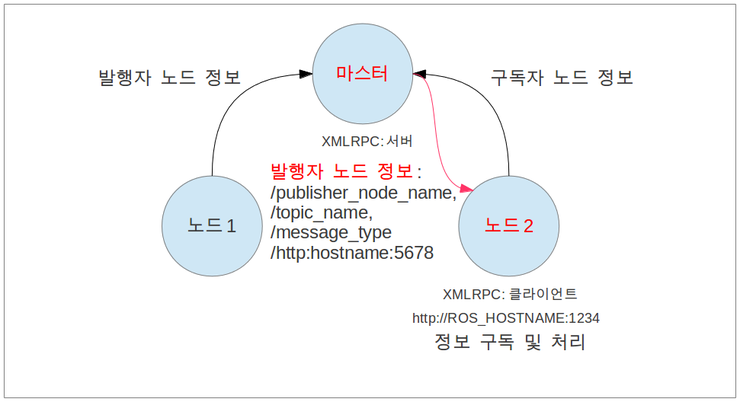
\includegraphics[width=0.9\columnwidth]{pictures/chapter4/notion4.png}
\caption{발행자 정보 알림}
\end{figure}

\newpage
%-------------------------------------------------------------------------------
\subsection{발행자 노드에 접속 요청}\index{발행자 노드에 접속 요청}

구독자 노드는 마스터로부터 받은 발행자 정보를 기반으로 발행자 노드에게 직접 접속 요청을 한다. 이때에 전송하는 정보로는 자신의 구독자 노드 이름, 토픽이름, 메시지방식(TCPROS 또는 UDPROS)이 있다. 발행자 노드와 구독자 노드는 XMLRPC 를 이용하여 통신하게 된다.

\begin{figure}[h]
\centering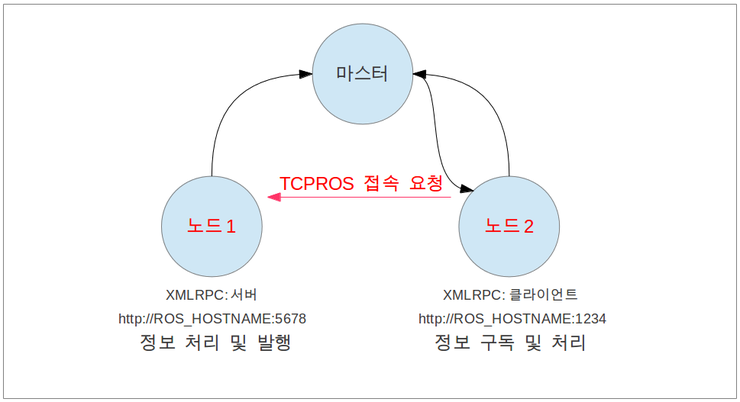
\includegraphics[width=0.9\columnwidth]{pictures/chapter4/notion5.png}
\caption{발행자 노드에 접속 요청}
\end{figure}

%-------------------------------------------------------------------------------
\subsection{발행자 노드에 접속 응답}\index{발행자 노드에 접속 응답}

발행자 노드는 구독자노드에게 접속 응답에 해당되는 자신의 TCP 서버의 정보인 URI주소와 포트를 전송한다. 발행자 노드와 구독자 노드는 XMLRPC 를 이용하여 통신하게 된다.

\begin{figure}[h]
\centering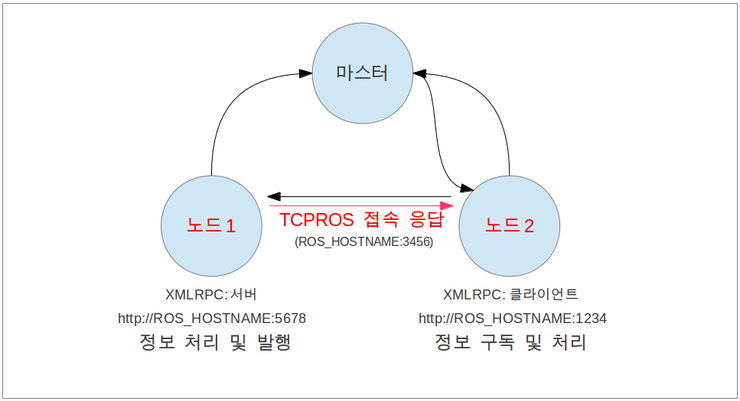
\includegraphics[width=0.9\columnwidth]{pictures/chapter4/notion6.png}
\caption{발행자 노드에 접속 응답}
\end{figure}

\newpage
%-------------------------------------------------------------------------------
\subsection{TCP 접속}\index{TCP 접속}

구독자 노드는 TCPROS를 이용하여 발행자노드에 대한 클라이언트를 만들고, 발행자노드와 직접 연결한다. (노드간의 통신 방식으로는 TCPROS라 하는 TCP/IP 방식을 이용한다.)

\begin{figure}[h]
\centering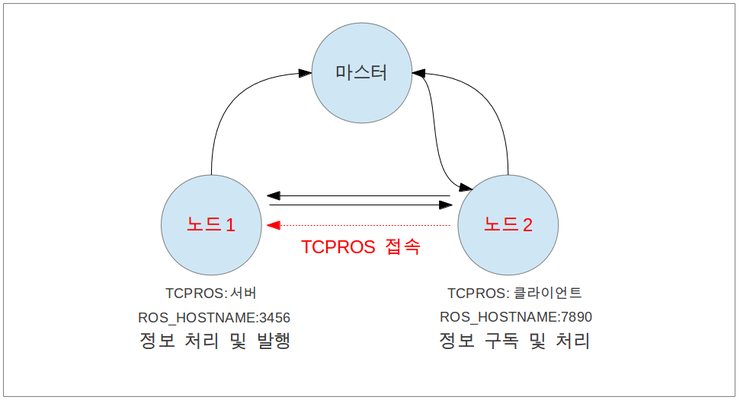
\includegraphics[width=0.9\columnwidth]{pictures/chapter4/notion7.png}
\caption{TCP 접속}
\end{figure}

%-------------------------------------------------------------------------------
\subsection{메시지 전송}\index{메시지 전송}

발행자 노드는 구독자 노드에게 정해진 메시지를 전송한다. (노드간의 통신 방식으로는 TCPROS라 하는 TCP/IP 방식을 이용한다.)

\begin{figure}[h]
\centering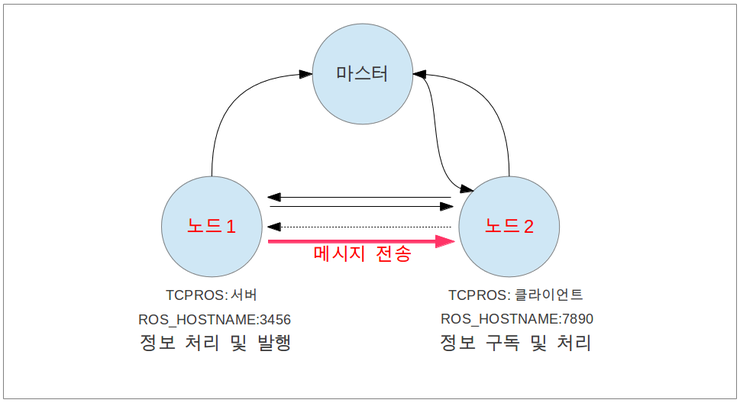
\includegraphics[width=0.9\columnwidth]{pictures/chapter4/notion8.png}
\caption{메시지 전송}
\end{figure}

\newpage
%-------------------------------------------------------------------------------
\subsection{서비스 요청 및 응답}\index{서비스 요청 및 응답}

위에서 설명한 내용은 메시지 통신중에 토픽에 해당된다. 토픽의 경우, 발행자 및 구독자가 중지하지 않는 이상, 메시지가 연속적으로 발행되고 구독하게 된다. 서비스의 경우에는 서비스를 요청하는 서비스 클라이언트와 서비스 요청을 받고 정해진 프로세스를 수행 및 응답하는 서비스 서버로 구분된다. 서비스는 토픽과 달리 1회에 한해 접속, 서비스 요청, 서비스 응답이 수행되고 서로간의 접속을 끊는다. 다시 필요한 경우 접속부터 다시 진행해야 한다. 

\begin{figure}[h]
\centering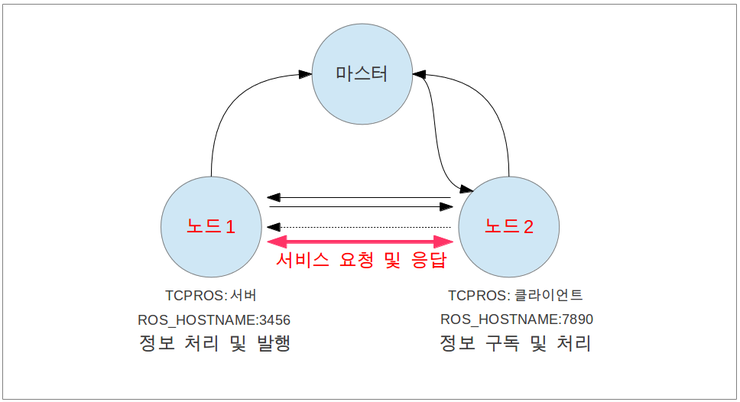
\includegraphics[width=0.7\columnwidth]{pictures/chapter4/notion9.png}
\caption{서비스 요청 및 응답}
\end{figure}

%-------------------------------------------------------------------------------
\subsection{예제}\index{예제}

이전 내용에서 우리는 turtlesim 을 이용하여 ROS의 구동을 테스트 해보았다. 이 테스트에서도 마스터 및 두 개의 노드가 사용되었고, 두 노드간에는 /turtle1/cmd\_vel 이라는 토픽을 이용하여 메시지 통신하고 있다. 이를 위해서 설명한 ROS 개념 맞추어 생각해보면 다음의 그림처럼 생각할 수 있다. 이전 ROS 동작 테스트 내용을 되새김해보며 ROS 개념을 다시 한번 생각해보자.

\begin{figure}[h]
\centering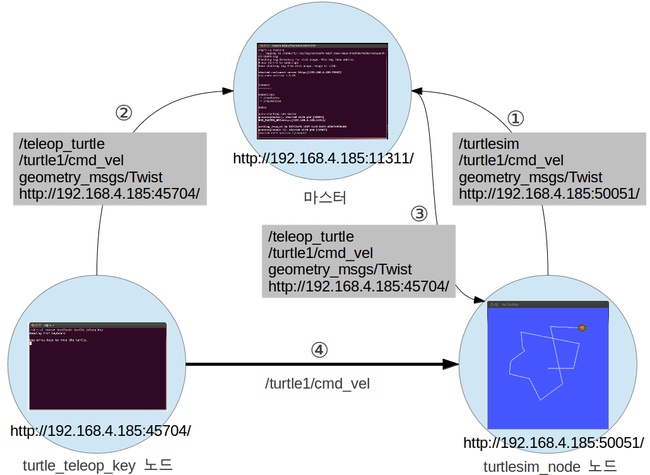
\includegraphics[width=0.8\columnwidth]{pictures/chapter4/notion10.png}
\caption{예제}
\end{figure}

\newpage
%-------------------------------------------------------------------------------
\section{ROS 파일시스템}\index{ROS 파일시스템}

%-------------------------------------------------------------------------------
\subsection{ROS의 파일 시스템}\index{ROS의 파일 시스템}
ROS의 파일 시스템에 대해서 설명하고자 한다. ROS는 ROS 설치 폴더와 사용자 작업 폴더로 구분된다. 
ROS 설치 폴더는 ROS의 데스크톱 버전을 설치하게 되면 /opt 폴더에 /ros 이라는 이름으로 폴더가 생성되고 그 안에 roscore를 포함한 핵심 유틸리티 및 rqt, rviz, 로봇 관련 라이브러리, 시뮬레이션, 네이게이션 등이 설치된다. 사용자는 이 부분의 파일들을 건들일은 거의 없다. 

사용자 작업 폴더는 사용자가 원하는 곳에 폴더를 생성가능한데 필자는 리눅스 사용자 폴더인 \textasciitilde/catkin\_ws/ (\textasciitilde/ 은 리눅스에서 /home/사용자명에 해당되는 폴더를 의미한다.) 에 설치할 것은 추천한다. 

\textbf{챕터~\ref{cha:RosInstall}~\nameref{cha:RosInstall}(pp.\pageref{cha:RosInstall})}에서 설명한 ROS Indigo 설치 및 ROS 개발 환경 구축를 진행했다는 가정하에 ROS 설치 폴더와 사용자 작업 폴더에 대한 상세한 내용을 설명하고자 한다.

%-------------------------------------------------------------------------------
\subsection{ROS 설치 폴더}\index{ROS 설치 폴더}

%-------------------------------------------------------------------------------
\subsubsection{설치 경로}\index{설치 경로}

ROS는 /opt/ros/[버전명] 폴더에 설치된다. 예를 들어, Indigo 버전을 설치하였을 경우 /opt/ros/indigo 가 ROS 설치 경로이다.

%-------------------------------------------------------------------------------
\subsubsection{파일 구성}\index{파일 구성}

다음의 그림과 같이 /opt/ros/indigo 의 폴더 아래에 bin, etc, include, lib, share 폴더 및 몇가지 환경 설정 파일들로 구성되어 있다. 

\begin{figure}[h]
\centering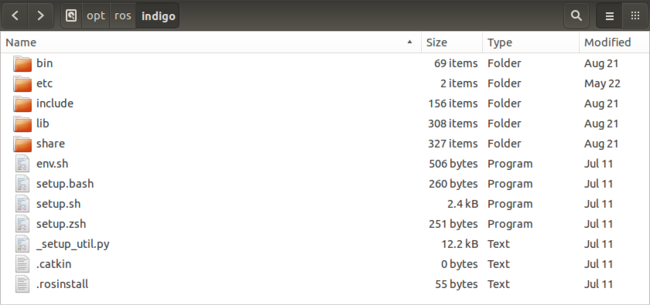
\includegraphics[width=0.7\columnwidth]{pictures/chapter4/folders.png}
\caption{ROS 파일 구성}
\end{figure}

%-------------------------------------------------------------------------------
\subsubsection{세부 내용}\index{세부 내용}
ROS이 폴더에는 ROS 설치시에 선택한 패키지를 포함한 ROS 구동 프로그램을 포함하고 있다. 세부 내용은 아래와 같다.

\begin{itemize}
\item /bin 실행가능한 바이너리 파일
\item /etc ROS 및 catkin 관련 설정파일
\item /include 헤더파일
\item /lib 라이브러리 파일
\item /share ROS 패키지
\item env.* 환경설정 파일
\item setup.* 환경설정 파일
\end{itemize}

%-------------------------------------------------------------------------------
\subsection{사용자 작업 폴더}\index{사용자 작업 폴더}

%-------------------------------------------------------------------------------
\subsubsection{사용자 작업 폴더 경로}\index{사용자 작업 폴더 경로}

사용자 작업 폴더는 사용자가 원하는 곳에 폴더를 생성가능하나 강좌의 원활한 진행을 위하여 리눅스 사용자 폴더인 \textasciitilde/catkin\_ws/ (\textasciitilde/ 은 리눅스에서 /home/사용자명에 해당되는 폴더를 의미한다.) 에 설치할 것은 추천한다. 즉, /home/사용자명/catkin폴더명 으로 설치하면된다. 예를들어 사용자명이 oroca라는 아이디이고 catkin폴더명은 catkin\_ws라고 설정하였다면 /home/oroca/catkin\_ws/ 폴더가 된다.

%-------------------------------------------------------------------------------
\subsubsection{파일 구성}\index{파일 구성}

다음의 그림과 같이 /home/사용자명/ 폴더의 아래에 catkin\_ws 라는 폴더가 있고, build, devel, src 폴더로 구성되어 있다. 

\begin{figure}[h]
\centering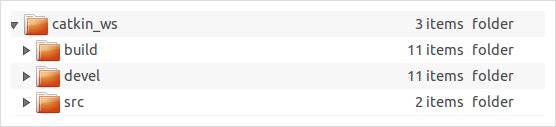
\includegraphics[width=0.65\columnwidth]{pictures/chapter4/folder_catkin_ws.png}
\caption{catkin workspace의 파일 구성}
\end{figure}

%-------------------------------------------------------------------------------
\subsubsection{세부 내용}\index{세부 내용}

이 폴더에는 사용자 작업 폴더로 사용자가 작성한 패키지 및 공개된 다른 개발자의 패키지를 저장하고 빌드하는 공간이다. 사용자는 이 폴더를 작업 폴더로 이용하며 ROS 관련된 내부분의 작업을 이 폴더안에서 하게된다. 세부 내용은 아래와 같다.

\vspace{\baselineskip}
\begin{itemize}[leftmargin=*]
\item /build catkin : 빌드 시스템의 빌드 환경 파일
\item /devel catkin : 빌드 시스템에 의해 빌드된 msg, srv 헤더파일 및 사용자 패키지 라이브러리 및 실행파일
\item /src : 사용자 패키지
\end{itemize}

%-------------------------------------------------------------------------------
\subsubsection{사용자 패키지}\index{사용자 패키지}

\textasciitilde/catkin\_ws/src 폴더에는 사용자가 사용하는 공간이다. 이 폴더에 사용자가 개발한 ROS 패키지 및 다른 개발자가 개발한 패키지를 저장하고 빌드하여 실행 파일을 생성해 낼 수 있다. ROS 빌드 시스템은 다음 강좌를 통해 저 자세히 알아 보도록 하고 이번 강좌에는 "이런 폴더와 파일로 구성되어 있구나" 라고 알아두고 넘어가기로 하자. 아래의 예제는 필자가 작성한 oroca\_ros\_tutorial 이라는 패키지를 작성한 후의 상태이다.

\begin{figure}[h]
\centering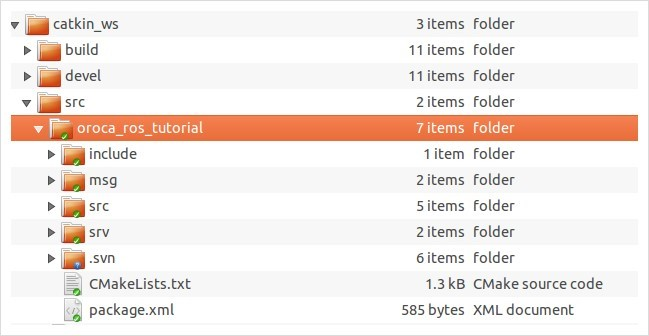
\includegraphics[width=0.65\columnwidth]{pictures/chapter4/folder_oroca_ros_tutorial.jpg}
\caption{사용자 패키지의 파일 구성}
\end{figure}

\begin{itemize}
\item /include 헤더파일
\item /launch ROS런치에 사용되는 스크립트
\item /node rospy용 스크립트
\item /msg 메시지 파일
\item /src 코드 소스 파일
\item /srv 서비스 파일
\item CMakeLists.txt 빌드 설정 파일
\item package.xml 패키지 설정 파일
\end{itemize}

%-------------------------------------------------------------------------------
\section{ROS 빌드 시스템}\index{ROS 빌드 시스템}
\label{sec:RosBuildSystem}

%-------------------------------------------------------------------------------
\subsection{ROS 빌드 시스템}\index{ROS 빌드 시스템}

ROS의 빌드 시스템은 기본적으로 CMake(Cross Platform Make)\footnote{CMake, wikipedia, http://ko.wikipedia.org/wiki/CMake} 를 이용하고 있고, 패키지 폴더에 CMakeLists.txt 라는 파일에 빌드 환경을 기술하고 있다. ROS에서는 CMake를 ROS에 맞도록 수정하여 ROS에 특화된 캐킨 빌드 시스템을 만들었다. 

ROS에서 CMake를 이용하고 있는 이유는 멀티플랫폼에서 ROS 패키지를 빌드할 수 있도록 위함이다. Make\footnote{Make, wikipedia, http://ko.wikipedia.org/wiki/Make}가 유닉스계열만 지원하는 것과 달리, CMake는 유닉스 계열인 리눅스, BSD, OS X 뿐만 아니라 윈도우 계열도 지원하기 때문이다. 또한, 마이크로소프트 비주얼 스튜디오도 지원하고 QT개발에도 쉽게 적용될 수 있다. 

더욱이, 캐킨 빌드 시스템은 ROS와 관련된 빌드, 패키지 관리, 패키지간의 의존관계 등을 편리하게 사용할 수 있도록 하고 있다. 

%-------------------------------------------------------------------------------
\subsection{패키지 생성}\index{패키지 생성}

ROS 패키지를 생성하기 위해서는 다음과 같은 명령어를 이용한다. "catkin\_create\_pkg" 는 사용자가 패키지를 작성할때 캐킨 빌드 시스템에 꼭 필요한 CMakeLists.txt 와 package.xml 를 포함한 패키지 폴더를 생성한다. 실제로 간단한 패키지를 작성해 보자.

\vspace{\baselineskip}
\begin{lstlisting}[language=ROS]
$ catkin_create_pkg %*[패키지이름] [의존하는패키지1] [의존하는패키지2] [의존하는패키지3]*)
\end{lstlisting}

%-------------------------------------------------------------------------------
\subsubsection{작업 폴더로 이동}\index{작업 폴더로 이동}

\vspace{\baselineskip}
\begin{lstlisting}[language=ROS]
$ cd ~/catkin_ws/src
\end{lstlisting}

%-------------------------------------------------------------------------------
\subsubsection{패키지 생성}\index{패키지 생성}

"my\_first\_ros\_pkg" 라는 이름의 패키지를 생성할 것이다. 

ROS에서는 패키지 이름에는 모두 소문자를 사용하며, 스페이스바와 같은 공백이 있으면 안된다. 그리고 일반적으로 하이픈(-) 대신에 밑줄(\_)을 사용하여 각 단어를 이어붙이는 것을 관례로 하고 있다. 

그리고 이번에는 의존하는 패키지로 "std\_msgs"와 "roscpp"를 옵션으로 달아주었다. ROS의 표준 메시지 패키지인 std\_msgs 와 ROS에서 C/C++을 사용하기 위하여 클라이언트라이브러인 roscpp를 사용하겠다는 것으로 패키지 생성에 앞어서 미리 설치해야한다는 의미이다. 이러한 의존하는 패키지의 설정은 패키지 생성할 때 지정할 수도 있지만, 생성 후 package.xml 에서 직접 입력하여도 된다.

\vspace{\baselineskip}
\begin{lstlisting}[language=ROS]
$ catkin_create_pkg my_first_ros_pkg std_msgs roscpp
\end{lstlisting}

위와 같이 패키지를 생성하였으면 "\textasciitilde/catkin\_ws/src"에 "my\_first\_ros\_pkg" 라는 패키지 폴더 및 ROS 패키지가 갖추어야할 기본 내부 폴더 및 CMakeLists.txt 와 package.xml가 생성된다. 다음과 같이 명령어로 ls 를 입력하여 내용을 보던가 윈도우의 탐색기와 같은 역할을 하는 GUI기반의 Nautilus를 이용하여 패키지 내부를 살펴보도록 하자.

\vspace{\baselineskip}
\begin{lstlisting}[language=ROS]
$ ls
include       %*.......... 인클루드 폴더*)
src           %*.......... 소스코드 폴더*)
CMakeLists.txt%*.......... 빌드 설정 파일*)
package.xml   %*.......... 패키지 설정 파일*)
\end{lstlisting}

\begin{figure}[h]
\centering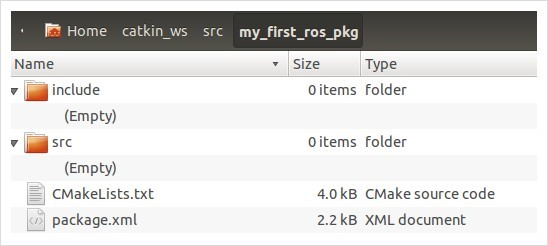
\includegraphics[width=0.6\columnwidth]{pictures/chapter4/new_package.jpg}
\caption{caption}
\end{figure}

%-------------------------------------------------------------------------------
\subsection{패키지 설정 파일 (package.xml) 수정}\index{패키지 설정 파일 (package.xml) 수정}

ROS의 필수 설정 파일 중 하나인 package.xml 은 패키지의 정보를 담은 XML 파일로써 패키지의 이름, 저작자, 라이선스, 의존성 패키지 등을 기술하고 있다. 처음에 아무런 수정을 가하지 않은 원본 파일은 다음과 같다.

\vspace{\baselineskip}
\lstinputlisting[language=XML, numbers=none, caption=package.xml]{./sources/package.xml}

\vspace{\baselineskip}
\begin{itemize}[leftmargin=*]
\item \textless{?xml}\textgreater~문서 분법을 정의하는 문구로 아래의 내용은 xml 버전 1.0을 따르고 있다는 것을 알리고 있다.
\item \textless{package}\textgreater~이 구문부터 \textless/package\textgreater 까지가 ROS 패키지 설정 부분이다.
\item \textless{name}\textgreater~패키지의 이름이다. 패키지 생성할때 입력한 패키지 이름이 사용된다. 다른 옵션도 마찬가지이지만 이는 사용자가 원할때 언제든지 변경할 수 있다.
\item \textless{version}\textgreater~패키지의 버전이다. 자유롭게 지정할 수 있다.
\item \textless{description}\textgreater~패키지의 간단한 설명이다. 
\item \textless{maintainer}\textgreater~패키지 관리자의 연락처를 기재한다.
\item \textless{license}\textgreater~라이선스를 기재한다. BSD, MIT, GPLv3, LGPLv3 등을 기재하면 된다. 오로카에서는 MIT를 사용하고 있다.
\item \textless{url}\textgreater~패키지를 설명하는 웹 페이지 또는 버그관리, 저장소 등의 주소를 기입한다. 이 종류에 따라 type에  website, bugtracker, repository 를 대입하면 된다. 참고로 url 태그는 옵션이다.
\item \textless{author}\textgreater~패키지 개발에 참여한 개발자를 적어주면 된다. 참고로 author 태그는 옵션이다.
\item \textless{buildtool\_depend}\textgreater~빌드 시스템의 의존성을 기술한다. 지금은 캐킨 빌드 시스템을 이용하고 있기 때문에 catkin 를 입력하면 된다.
\item \textless{build\_depend}\textgreater~패키지를 빌드할 때 의존하는 패키지명을 적어준다.
\item \textless{run\_depend}\textgreater~패키지를 실행할 때 의존하는 패키지명을 적어준다.
\item \textless{test\_depend}\textgreater~패키지를 테스트할때 의존하는 패키지명을 적어준다. 테스트이외에는 사용하지 않는다.
\item \textless{export}\textgreater~ROS에서 명시하지 않은 태그명을 사용할때 쓰인다. 일반적인 경우 쓸일이 없다.
\item \textless{metapackage/}\textgreater~export 태그 안에서 사용하는 공식적인 태그로 현재의 패키지가 메타패키지의 경우 이를 선언한다.
\end{itemize}

\vspace{\baselineskip}
\noindent
필자는 다음과 같이 패키지 설정 파일(package.xml)을 수정하였다. 여러분은 자신에 맞게 수정해보도록 하자.

\vspace{\baselineskip}
\begin{lstlisting}[language=XML]
<?xml version="1.0"?>
<package>
  <name>my_first_ros_pkg</name>
  <version>0.0.1</version>
  <description>The my_first_ros_pkg package</description>
 
  <maintainer email="passionvirus@gmail.com">Yoonseok Pyo</maintainer>
  <license>MIT</license>
  <url type="website">http://cafe.naver.com/openrt/2500</url>
  <url type="repository">https://github.com/oroca/oroca_ros_tutorials.git</url>
  <author email="passionvirus@gmail.com">Yoonseok Pyo</author>
 
  <buildtool_depend>catkin</buildtool_depend>
 
  <build_depend>std_msgs</build_depend>
  <build_depend>roscpp</build_depend>
 
  <run_depend>std_msgs</run_depend>
  <run_depend>roscpp</run_depend>
 
  <export>
  </export>
</package>
\end{lstlisting}

%-------------------------------------------------------------------------------
\subsection{빌드 설정 파일 (CMakeLists.txt) 수정}\index{빌드 설정 파일 (CMakeLists.txt) 수정}

ROS의 빌드 시스템인 캐킨은 기본적으로 CMake를 이용하고 있어서 패키지 폴더에 CMakeLists.txt 라는 파일에 빌드 환경을 기술하고 있다. 이는 실행 파일 생성, 의존성 패키지 우선 빌드, 링크 생성 등을 설정하게 되어 있다. 처음에 아무런 수정을 가하지 않은 원본 파일은 다음과 같다.

\lstinputlisting[language=make, numbers=none, caption=CMakeLists.txt]{./sources/CMakeLists.txt}

\noindent
빌드 설정 파일 (CMakeLists.txt)의 각 옵션들은 다음과 같다.\\

운영체제에 설치되어 있는 cmake의 최소한의 버전이다. 현재에는 2.8.3 버전으로 명시되어 있다. 이 보다 낮은 cmake를 사용하는 경우에는 버전 업데이트를 해줘야 한다.
\begin{lstlisting}[language=make]
cmake_minimum_required(VERSION 2.8.3)
\end{lstlisting}

패키지의 이름이다. package.xml 에서 입력한 패키지 이름을 그대로 사용하자.
\begin{lstlisting}[language=make]
project(my_first_ros_pkg)
\end{lstlisting}

캐킨 빌드를 할 때 요구되는 구성요소 패키지이다. 현재 의존성 패키지로 roscpp 및 std\_msgs가 추가되어 있다. 여기에 입력된 패키지가 없는 경우 캐킨 빌드할 때 사용자에게 에러가 표시된다. 즉, 사용자가 만든 패키지가 의존하는 패키지를 먼저 설치하게 만드는 옵션이다.
\begin{lstlisting}[language=make]
find_package(catkin REQUIRED COMPONENTS
  roscpp
  std_msgs
)
\end{lstlisting}

ROS 이외의 패키지를 사용하는 경우에 사용되는 방법이다. 예를들어 다음의 경우, Boost를 사용할때 system 이라는 패키지가 설되어 있어야 한다. 기능은 위에서 설명한 의존하는 패키지를 먼저 설치하게 만드는 옵션이다.
\begin{lstlisting}[language=make]
find_package(Boost REQUIRED COMPONENTS system)
\end{lstlisting}

파이썬을 사용할 때 설정하는 옵션이다. 파이썬은 cmake를 사용할 필요없는 스크립트 언어이지만 패키지의 호환성을 위해 아래와 같이 독자적인 설정을 하게 되어 있다.
\begin{lstlisting}[language=make]
catkin_python_setup()
\end{lstlisting}

사용하는 메시지 파일을 추가하는 옵션이다. FILES를 사용하면 패키지 폴더의 msg 폴더안의 .msg 파일들을 참조하게 된다. 다음의 예제에서는 Message1.msg 및 Message2.msg 의 메시지 파일을 이용하겠다는 옵션이다.
\begin{lstlisting}[language=make]
add_message_files(
  FILES
  Message1.msg
  Message2.msg
)
\end{lstlisting}

사용하는 서비스 파일을 추가하는 옵션이다. FILES를 사용하면 패키지 폴더의 srv 폴더안의 .srv 파일들을 참조하게 된다. 다음의 예제에서는 Service1.srv 및 Service2.srv 의 서비스 파일을 이용하겠다는 옵션이다.
\begin{lstlisting}[language=make]
add_service_files(
  FILES
  Service1.srv
  Service2.srv
)
\end{lstlisting}

의존하는 메시지를 사용하겠다는 옵션이다. 다음의 예제에서는 DEPENDENCIES 옵션에 의하여 std\_msgs 라는 메시지 패키지를 사용하겠다는 설정이다.
\begin{lstlisting}[language=make]
generate_messages(
  DEPENDENCIES
  std_msgs
)
\end{lstlisting}

캐킨 빌드 옵션이다. "INCLUDE\_DIRS"는 뒤에 설정한 패키지 내부 폴더인 "include"의 헤더파일을 사용하겠다는 설정이다. "LIBRARIES"는 뒤에 설정한 패키지의 라이브러리를 사용하겠다는 설정이다. "CATKIN\_DEPENDS" 캐킨 빌드할 때 의존하는 패키지들이다. 현재 roscpp 및 std\_msgs가 의존하고 있다는 설정이다. "DEPENDS" 시스템 의존 패키지를 기술하는 설정이다.
\begin{lstlisting}[language=make]
catkin_package(
 INCLUDE_DIRS include
 LIBRARIES my_first_ros_pkg
 CATKIN_DEPENDS roscpp std_msgs
 DEPENDS system_lib
)
\end{lstlisting}

인클루드 폴더를 지정할 수 있는 옵션이다. 현재 \$\{catkin\_INCLUDE\_DIRS\} 라고 설정되어 있는데 이는 각 패키지안의 "include" 폴더를 의미하고 이 안의 헤더파일을 이용 하겠다는 설정이다.
\begin{lstlisting}[language=make]
include_directories(
  ${catkin_INCLUDE_DIRS}
)
\end{lstlisting}

cpp 라이브러리를 선언한다. src/\$\{PROJECT\_NAME\}/my\_first\_ros\_pkg.cpp 파일을 참조하여 my\_first\_ros\_pkg 라는 라이브러리를 생성하게 된다.
\begin{lstlisting}[language=make]
add_library(my_first_ros_pkg
  src/\${PROJECT_NAME}/my_first_ros_pkg.cpp
)
\end{lstlisting}

cpp 실행 파일을 선언한다. src/my\_first\_ros\_pkg\_node.cpp 파일을 참조하여 my\_first\_ros\_pkg\_node 라는 실행파일을 생성한다.
\begin{lstlisting}[language=make]
add_executable(my_first_ros_pkg_node src/my_first_ros_pkg_node.cpp)
\end{lstlisting}

패키지를 빌드하기 앞서서 생성해야할 메시지 헤더파일이 있을 경우 빌드전에 우선적으로 메시지를 생성하라는 설정이다. 현재 my\_first\_ros\_pkg\_generate\_messages\_cpp 를 우선적으로 빌드하고 my\_first\_ros\_pkg\_node 를 빌드하게 하는 설정이다.
\begin{lstlisting}[language=make]
add_dependencies(my_first_ros_pkg_node my_first_ros_pkg_generate_messages_cpp)
\end{lstlisting}

my\_first\_ros\_pkg\_node 를 생성하기 앞서서 링크해야하는 라이브러리 및 실행파일을 링크해주는 옵션이다.
\begin{lstlisting}[language=make]
target_link_libraries(my_first_ros_pkg_node
  \${catkin_LIBRARIES}
)
\end{lstlisting}

\noindent
필자는 다음과 같이 빌드 설정 파일(CMakelists.txt)을 수정하였다. 여러분은 자신에 맞게 수정해보도록 하자.

\begin{lstlisting}[language=make]
cmake_minimum_required(VERSION 2.8.3)
project(my_first_ros_pkg)
 
find_package(catkin REQUIRED COMPONENTS
  roscpp
  std_msgs
)
 
catkin_package(
  INCLUDE_DIRS include
  CATKIN_DEPENDS roscpp std_msgs
  DEPENDS system_lib
)
 
include_directories( ${catkin_INCLUDE_DIRS} )
 
add_executable(hello_world_node src/hello_world_node.cpp)
add_dependencies(hello_world_node my_first_ros_pkg_generate_messages_cpp)
target_link_libraries(hello_world_node ${catkin_LIBRARIES})
\end{lstlisting}

\newpage
%-------------------------------------------------------------------------------
\subsection{소스코드 작성}\index{소스코드 작성}

\vspace{\baselineskip}
\begin{lstlisting}[language=make]
add\_executable(hello\_world\_node src/hello\_world\_node.cpp)
\end{lstlisting}

위에서 설명한 CMakelists.txt 파일의 실행 파일 생성 부분(add\_executable)에서 위와 같이 설정해 놓았다. 즉, 패키지의 "src" 폴더에 있는 "hello\_world\_node.cpp" 소스 코드를 참고하여 "hello\_world\_node" 라는 실행 파일을 생성하라는 설정이다. 여기서, "hello\_world\_node.cpp" 소스코드가 없기에 간단한 예제로 하나 작성해 보자. 다음의 예제에서는 nano라는 에디터를 사용하였으나 vi, gedit, qtcreator 등 자신이 원하는 편집기를 이용하면 된다.

\vspace{\baselineskip}
\begin{lstlisting}[language=ROS]
$ cd /src     %* //여기서 src 는 자신의 패키지 폴더안의 src 라는 소스코드를 담는 폴더를 말한다.*)
$ nano hello_world_node.cpp
\end{lstlisting}

\begin{lstlisting}[language=C++]
#include <ros/ros.h>
#include <std_msgs/String.h>

#include <sstream>

int main(int argc, char **argv)
{
  ros::init(argc, argv, "hello_world_node");
  ros::NodeHandle nh;
  ros::Publisher chatter_pub = nh.advertise<std_msgs::String>("say_hello_world", 1000);

  ros::Rate loop_rate(10);
  int count = 0;
  while (ros::ok())
  {
    std_msgs::String msg;
    std::stringstream ss;
    ss << "hello world " << count;
    msg.data = ss.str();
    ROS_INFO("%s", msg.data.c_str());
    chatter_pub.publish(msg);
    ros::spinOnce();
    loop_rate.sleep();
    ++count;
  }
  return 0;
}
\end{lstlisting}

%-------------------------------------------------------------------------------
\subsection{패키지 빌드}\index{패키지 빌드}

이제 패키지 빌드를 위한 모든 작업이 완료되었다.  빌드에 앞서서 다음의 명령어로 ROS 패키지의 프로파일을 갱신시켜주자. 앞서 제작한 우리의 패키지를 ROS 패키지 목록에 반영시켜주는 명령어이다. 필수 사항은 아니지만 새로 패키지를 생성한 후에 갱신해주면 이용하기 편하다.

\vspace{\baselineskip}
\begin{lstlisting}[language=ROS]
$ rospack profile
\end{lstlisting}

\noindent
다음은 캐킨 빌드 이다. 캐킨 작업 폴더로 이용하여 캐킨 빌드를 해주자.

\vspace{\baselineskip}
\begin{lstlisting}[language=ROS]
$ cd ~/catkin_ws && catkin_make
%*또는*)
$ cm
\end{lstlisting}

\noindent
이전 강좌인 "ROS 강좌 : 06. ROS 개발 환경 구축"에서 언급했듯이 .bashrc 파일에 alias \verb|cm='cd ~/catkin_ws && catkin_make'| 라고 설정해두면 터미널 창에서 "cm" 이라는 간단한 명령어로 위의 명령어를 대체할 수 있다. 유용한 만큼 이전 강좌를 보고 꼭 설정해 두도록 하자.

%-------------------------------------------------------------------------------
\subsection{노드 실행}\index{노드 실행}

에러 없이 빌드가 완료되었으면 "\textasciitilde/catkin\_ws/devel/lib/my\_first\_ros\_pkg" 에 "hello\_world\_node" 라는 파일이 생성되었을 것이다. 한번 확인해 보자.

다음 단계는 노드를 실행하는 것인데 노드 실행에 앞서서 roscore를 구동하자. ROS의 모든 노드는 roscore를 구동한 후에 이용할 수 있다.

\vspace{\baselineskip}
\begin{lstlisting}[language=ROS]
$ roscore
\end{lstlisting}

\noindent
마지막으로 새로운 터미널창을 열어 아래의 명령어로 노드를 실행해보자. my\_first\_ros\_pkg 라는 패키지의 hello\_world\_node 라는 노드를 실행하라는 명령어이다.

\vspace{\baselineskip}
\begin{lstlisting}[language=ROS]
$ rosrun my_first_ros_pkg hello_world_node 
[ INFO] [1380598894.131775283]: hello world 0
[ INFO] [1380598894.231826916]: hello world 1
[ INFO] [1380598894.331798085]: hello world 2
[ INFO] [1380598894.431796634]: hello world 3
[ INFO] [1380598894.531808660]: hello world 4
[ INFO] [1380598894.631800431]: hello world 5
[ INFO] [1380598894.731805683]: hello world 6
\end{lstlisting}

\noindent
노드를 실행하게 되면 위와 같이 hello world 1, 2 ,3 과 같은 메시지가 발행되는 것을 볼 수 있을 것이다. 이번 강좌는 ROS의 빌드 시스템을 설명하기 위한 것이니 노드의 소스코드에 관해서는 다음 강좌를 통해 알아보도록 하자.


%-------------------------------------------------------------------------------
% -*- root: main.tex -*-

%-------------------------------------------------------------------------------
\chapterimage{chapter_head_5.pdf} 

%-------------------------------------------------------------------------------
\chapter{ROS 명령어}

%-------------------------------------------------------------------------------
\section{ROS 명령어 정리}\index{ROS 명령어 정리}
\label{sec:RosCommand}

ROS는 쉘(shell)환경에서 명령어로 파일 시스템 이용, 소스코드 편집, 빌드, 디버깅, 패키지 관리 등을 처리할 수 있다. ROS를 제대로 사용하기 위해서는 기본적인 리눅스 명령어 이외에도 ROS만의 고유한 명령어\footnote{ROS, CommandLineTools, http://wiki.ros.org/ROS/CommandLineTools}들을 익힐 필요가 있다. ROS 명령어로는 다음과 같이 다양하게 존재한다. 

처음부터 모든 명령어를 숙련하게 사용할 수 없겠지만, 다음의 내용을 보고 필요할 때마다 이용하면 되겠다. 처음에는 익숙하지 않아서 불편하게 느껴질 수 있겠지만, 사용하면 사용할 수록 매우 빠르고 편하게 각종 기능을 명령어로 처리하는 자신의 모습을 보게 될 것이다.

ROS의 다양한 명령어를 숙달하기 위하여 본 강좌에서는 우선 각 명령어의 기능을 간단히 설명하고, 하나 하나 예제를 들어가며 소개하도록 하겠다. 그리고 각 명령어의 사용 빈도 및 중요도를 고려하여 필자가 별표로 점수를 매겨두었다. 별표가 많은 명령어의 경우, 사용 빈도수가 높고 중요한 명령어이니 꼭 익혀두기로 하자.

\vspace{\baselineskip}
\noindent
\textbf{[ROS 쉘 명령어]}
\begin{description}
\item[roscd] (★★★) ros+cd(changes directory) : ROS 패키지 또는 스택의 디렉토리 변경 명령어
\item[rospd] (☆☆☆) ros+pushd : ROS 디렉토리 인덱스에 디렉토리 추가
\item[rosd] (☆☆☆) ros+directory : ROS 디렉토리 인덱스 확인 명령어
\item[rosls] (★☆☆) ros+ls(lists files) : ROS 패키지의 파일 리스트를 확인하는 명령어
\item[rosed] (★☆☆) ros+ed(editor) : ROS 패키지의 파일을 편집하는 명령어
\item[roscp] (☆☆☆) ros+cp(copies files) : ROS 패키지의 파일 복사하는 명령어
\end{description}

\vspace{\baselineskip}
\noindent
\textbf{[ROS 실행 명령어]}
\begin{description}
\item[roscore] (★★★) ros+core : master (ROS 네임 서비스) + rosout (stdout/stderr) + parameter server (매개변수관리)
\item[rosrun] (★★★) ros+run : 패키지의 노드를 실행하는 명령어
\item[roslaunch] (★★★) ros+launch : 패키지의 노드를 복수개 실행하는 명령어
\item[rosclean] (★☆☆) ros+clean : ros 로그 파일을 체크하거나 삭제하는 명령어
\end{description}

\vspace{\baselineskip}
\noindent
\textbf{[ROS 정보 명령어]}
\begin{description}
\item[rostopic] (★★★) ros+topic : ROS 토픽 정보를 확인하는 명령어
\item[rosservice] (★★★) ros+service : ROS 서비스 정보를 확인하는 명령어
\item[rosnode] (★★★) ros+node : ROS의 노드 정보를 얻는 명령어
\item[rosparam] (★★★) ros+param(parameter) : ROS 파라미터 정보를 확인, 수정 가능한 명령어
\item[rosmsg] (★★☆) ros+msg : ROS 메세지 선언 정보를 확인하는 명령어
\item[rossrv] (★★☆) ros+srv : ROS 서비스 선언 정보를 확인하는 명령어
\item[roswtf] (☆☆☆) ros+wtf : ROS 시스템을 검사하는 명령어
\item[rosversion] (★☆☆) ros+version : ros 패키및 배포 릴리즈 버전의 정보를 확인하는 명령어
\item[rosbag] (★★★) ros+bag : ROS 메세지를 기록, 재생하는 명령어
\end{description}

\vspace{\baselineskip}
\noindent
\textbf{[ROS 캐킨 명령어]}
\begin{description}
\item[catkin\_create\_pkg] (★★★) 캐킨 빌드 시스템에 의한 패키지 자동 생성
\item[catkin\_eclipse] (★★☆) 캐킨 빌드 시스템에 의해 생성된 패키지를 이클립스에서 사용할 수 있도록 변경하는 명령어
\item[catkin\_find] (☆☆☆) 캐킨 검색
\item[catkin\_generate\_changelog] (☆☆☆) 캐킨 변경로그 생성
\item[catkin\_init\_workspace] (★☆☆) 캐킨 빌드 시스템의 작업폴더 초기화
\item[catkin\_make] (★★★) 캐킨 빌드 시스템을 기반으로한 빌드 명령어
\end{description}

\vspace{\baselineskip}
\noindent
\textbf{[ROS 패키지 명령어]}
\begin{description}
\item[rosmake] (☆☆☆) ros+make : ROS package 를 빌드한다. (구 ROS 빌드 시스템에서 사용됨)
\item[rosinstall] (★☆☆) ros+install : ROS 추가 패키지 설치 명령어
\item[roslocate] (☆☆☆) ros+locate : ROS 패키지 정보 관련 명령어 
\item[roscreate-pkg] (☆☆☆) ros+create-pkg : ROS 패키지를 자동 생성하는 명령어 (구 ROS 빌드 시스템에서 사용됨)
\item[rosdep] (★☆☆) ros+dep(endencies) : 해당 패키지의 의존성 파일들을 설치하는 명령어
\item[rospack] (★★☆) ros+pack(age) : ROS 패키지와 관련된 정보를 알아보는 명령어
\end{description}

%-------------------------------------------------------------------------------
\section{ROS 쉘 명령어}\index{ROS 쉘 명령어}

ROS 쉘 명령어는 일명 rosbash\footnote{ROS, rosbash, http://wiki.ros.org/rosbash}라고 부른다. 이는 리눅스에서 일반적으로 사용하는 bash 쉘 명령어를 ROS에서 사용하는 방법이다. 주로 ros 라는 접두사에 cd, pd, d, ls, ed, cp, run 등의 접미사를 붙여서 사용하게 된다. 이와 관련된 명령어들을 아래에 소개한다.  

\vspace{\baselineskip}
\noindent
\begin{description}
\item[roscd] (★★★) ros + cd (changes directory) 
\item[rospd] (☆☆☆) ros + pushd 
\item[rosd] (☆☆☆) ros + directory
\item[rosls] (★☆☆) ros + ls (lists files)
\item[rosed] (★☆☆) ros + ed (editor)
\item[roscp] (☆☆☆) ros+cp (copies files)
\item[rosrun] (★★★) ros+run 
\end{description}

\vspace{\baselineskip}
\noindent
이 중, 비교적 자주 사용되는 roscd, rosls, rosed 명령어에 대해서 자세히 알아보자.

\vspace{\baselineskip}
\noindent
※ rosrun 은 rosbash 에 포함되나 의미상 ROS 실행 명령어이기 때문에 여기서 다루도록 한다.

\newpage
%-------------------------------------------------------------------------------
\subsection{roscd : ROS 디렉토리 이동}\index{roscd : ROS 디렉토리 이동}

\setcounter{num}{0}

\stepcounter{num}\circled{\thenum} 사용법
\begin{lstlisting}[language=ROS]
roscd [%*패키지이름*)]
\end{lstlisting}

\noindent
\stepcounter{num}\circled{\thenum} 사용예
\begin{lstlisting}[language=ROS]
$ roscd turtlesim
\end{lstlisting}

\noindent
\stepcounter{num}\circled{\thenum} 결과값
\begin{lstlisting}[language=ROS]
/opt/ros/indigo/share/turtlesim$
\end{lstlisting}

\noindent
사용예에서 처럼, turtlesim 이라는 패키지 이름을 매개변수로 넣어주고 실행하게 되면 지정된 패키지가 저장된 폴더로 이동하게 된다. 현재 결과에서는 turtlesim 이라는 패키지가 ROS가 설치되어 있는 폴더에 있으므로 위와 같이 나왔으나, 자신이 작성한 패키지의 이름을 매개변수로 넣어주면 자신이 설정한 패키지의 디렉토리로 이동할 수도 있다. 명령어 기반의 ROS를 사용하는데 있어서 매우 사용빈도가 높은 명령어이다.

\vspace{\baselineskip}
\noindent
※ 위와 같은 실행 및 결과를 위해서는 관련 패키지인 ros-indigo-turtlesim 패키지가 설치되어 있어야 한다. 만약 설치되어 있지 않은 경우 설치하도록 하자. 설치 명령어는 sudo apt-get install ros-indigo-turtlesim  이다.

%-------------------------------------------------------------------------------
\subsection{rosls : ROS 리스트 파일}\index{rosls : ROS 리스트 파일}

\setcounter{num}{0}

\stepcounter{num}\circled{\thenum} 사용법
\begin{lstlisting}[language=ROS]
rosls [%*패키지이름*)]
\end{lstlisting}

\noindent
\stepcounter{num}\circled{\thenum} 사용예
\begin{lstlisting}[language=ROS]
$ rosls turtlesim
\end{lstlisting}

\noindent
\stepcounter{num}\circled{\thenum} 결과값
\begin{lstlisting}[language=ROS]
$ rosls turtlesim/
cmake  images  msg  package.xml  srv
\end{lstlisting}

\noindent
지정한 ROS 패키지의 파일 리스트를 확인하는 명령어이다. roscd 명령어를 이용하여 해당 패키지로 이동후에 일반 ls 명령어로 같은 기능을 수행할 수도 있지만, 간혹 바로 확인할 필요가 있을경우에 사용된다. 사용 빈도수는 매우 떨어진다.

%-------------------------------------------------------------------------------
\subsection{rosed : ROS 편집 명령어}\index{rosed : ROS 편집 명령어}

\setcounter{num}{0}

\stepcounter{num}\circled{\thenum} 사용법
\begin{lstlisting}[language=ROS]
rosed [%*패키지이름*)] [%*파일이름*)]
\end{lstlisting}

\noindent
\stepcounter{num}\circled{\thenum} 사용예
\begin{lstlisting}[language=ROS]
$ rosed turtlesim package.xml 
\end{lstlisting}

\noindent
turtlesim 패키지의 package.xml 를 편집하고자 할때 사용하는 명령어이다. 이를 실행하면 사용자가 설정한 에디터로 해당 파일을 열게된다. 급하게 간단히 파일을 수정하고자 할때 사용된다. 사용되는 에디터는 "~/.bashrc" 파일에 export EDITOR='emacs -nw' 와 같이 지정하여 사용가능하다. 필자는 비교적 단순한 편집일 경우 이를 사용한다. 프로그램 작성과 같은 작업 rosed 이외에 자신만의 개발환경을 사용하기를 추천한다.

\vspace{\baselineskip}
\noindent
\stepcounter{num}\circled{\thenum} 결과값
\begin{lstlisting}[language=ROS]
%*사용자가 지정해둔 에디터를 이용하여 해당 파일을 열게된다.*)
\end{lstlisting}

\noindent
바로 명령어창에서 수정이 필요한 단순한 작업에서 많이 사용되지만, 그 이외의 프로그램 작업등에는 비추천이다. 전체적인 사용 빈도수는 매우 떨어진다.

%-------------------------------------------------------------------------------
\section{ROS 실행 명령어}\index{ROS 실행 명령어}

ROS 실행 명령어\footnote{http://wiki.ros.org/rosbash}는 ROS 노드의 실행을 주관한다. 무엇보다 필수는 roscore로 노드간의 네임 서버로 사용된다. 그리고 실행명령어로는 rosrun 및 roslaunch가 있다. rosrun 는 하나의 노드를 실행하게 되며, roslaunch 는 하나이상의 노드를 실행할때 사용된다. 그리고 rosclean 는 노드 실행시 기록되는 로그의 삭제에 사용되는 명령어이다.

\vspace{\baselineskip}
\noindent
\begin{description}
\item[roscore] (★★★) ros+core : master (ROS 네임 서비스) + rosout (stdout/stderr) + parameter server (매개변수관리)
\item[rosrun] (★★★) ros+run : 패키지의 노드를 실행하는 명령어
\item[roslaunch] (★★★) ros+launch : 패키지의 노드를 복수개 실행하는 명령어
\item[rosclean] (★☆☆) ros+clean : ros 로그 파일을 체크하거나 삭제하는 명령어
\end{description}

\newpage
%-------------------------------------------------------------------------------
\subsection{roscore : ROS 코어 실행}\index{roscore : ROS 코어 실행}
\label{subsec:Roscore}

ROS코어\footnote{http://wiki.ros.org/roscore}는 노드들간의 메시지 통신에서 연결 정보를 관리하는 마스터로서, ROS를 사용하기 위해서 제일 먼저 구동해야하는 필수 요소이다. 다음과 같이 "roscore"라는 실행 명령어로 ROS 마스터는 구동되며, XMLRPC으로 서버를 구동하게 된다. 마스터는 노드간의 접속을 위하여 노드들의 이름, 토픽 및 서비스의 이름, 메시지 형태, URI 주소 및 포트를  등록받고, 요청이 있을 경우 이 정보를 다른 노드에게 알려주는 역할을 한다. 

\setcounter{num}{0}

\vspace{\baselineskip}
\noindent
\stepcounter{num}\circled{\thenum} 사용법
\begin{lstlisting}[language=ROS]
roscore [%*옵션*)]
\end{lstlisting}

\noindent
\stepcounter{num}\circled{\thenum} 사용예
\begin{lstlisting}[language=ROS]
$ roscore
\end{lstlisting}

\noindent
위의 명령어로 ROS 코어를 실행하게되면 사용자가 설정해둔 ROS\_MASTER\_URI 를 마스터 URI로 하여, 마스터를 기동하게 된다. ROS\_MASTER\_URI 은 "~/.bashrc" 에서 사용자가 설정하도록 되어있다.

\vspace{\baselineskip}
\noindent
\stepcounter{num}\circled{\thenum} 결과값
\begin{lstlisting}[language=ROS]
$ roscore
... logging to /home/rts/.ros/log/fefe3f-63dc-fege-a5a1-f3r3df3e44/roslaunch-rts-3547.log
Checking log directory for disk usage. This may take awhile.
Press Ctrl-C to interrupt
Done checking log file disk usage. Usage is <1GB.
started roslaunch server http://192.168.4.100:57385/
ros_comm version 1.11.9

SUMMARY
========
PARAMETERS
 * /rosdistro: indigo
 * /rosversion: 1.11.9

NODES

auto-starting new master
process[master]: started with pid [3560]
ROS_MASTER_URI=http://192.168.4.100:11311/

setting /run_id to fefe3f-63dc-fege-a5a1-f3r3df3e44
process[rosout-1]: started with pid [3575]
started core service [/rosout]
\end{lstlisting}

\noindent
위 결과에서 /home/rt/.ros/log/ 폴더에 로그들이 저장되고 있다는 것과 "Ctrl-C" 키로 ROS 코어를 종료할 수 있다느 것, roslaunch server, ROS\_MASTER\_URI 등의 정보, /rosdistro 및 /rosversion의 파라미터 서버, /rosout 의 서비스, /rosout 노드가 실행되었음을 알수 있다.


%-------------------------------------------------------------------------------
\subsection{rosrun : ROS 노드 실행}\index{rosrun : ROS 노드 실행}

rosrun\footnote{http://wiki.ros.org/rosbash}은 지정한 패키지의 하나의 노드를 실행하는 명령어이다. turtlesim 이라는 패키지의 turtlesim\_node 이라는 노드를 실행하는 명령어이다. rosrun은 지정한 패키지의 하나의 노드를 실행시킨다. 

\setcounter{num}{0}

\vspace{\baselineskip}
\noindent
\stepcounter{num}\circled{\thenum} 사용법
\begin{lstlisting}[language=ROS]
rosrun [%*패키지이름*)] [%*노드이름*)]
\end{lstlisting}

\noindent
\stepcounter{num}\circled{\thenum} 사용예
\begin{lstlisting}[language=ROS]
$ rosrun turtlesim turtlesim_node 
\end{lstlisting}

\noindent
\stepcounter{num}\circled{\thenum} 결과값
\begin{lstlisting}[language=ROS]
$ rosrun turtlesim turtlesim_node 
[INFO] [1383445615.677782380]: Starting turtlesim with node name /turtlesim
[INFO] [1383445615.686475328]: Spawning turtle [turtle1] at x=[5.544445], y=[5.544445], theta=[0.000000]
\end{lstlisting}

\begin{figure}[h]
\centering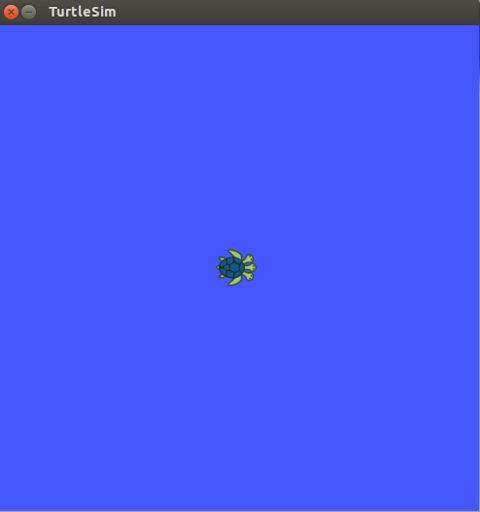
\includegraphics[width=0.7\columnwidth]{pictures/chapter5/term_rosrun.png}
\caption{turtlesim\_node 노드를 실행한 모습}
\end{figure}

\newpage
%-------------------------------------------------------------------------------
\subsection{roslaunch : ROS 노드 복수 실행}\index{roslaunch : ROS 노드 복수 실행}

roslaunch\footnote{http://wiki.ros.org/roslaunch} 지정한 패키지의 하나이상의 노드를 실행하는 명령어이다. 아래와 같이 openni\_launch를 구동하는 것만으로도 camera\_nodelet\_manager, depth\_metric, depth\_metric\_rect, depth\_points 등의 20개 이상의 노드 및 10여개의 파라미터 서버가 실행된다. 이렇듯 런치파일을 이용한 실행은 하나의 패키지의 다수의 노드를 실행하는데 매우 유용하며, ROS에서는 매우 많이 사용되는 실행 방법이다. 이때 사용되는 .launch 파일 작성에 대해서는 \textbf{섹션~\ref{sec:HowToUseTheRoslaunch}~\nameref{sec:HowToUseTheRoslaunch}(pp.\pageref{sec:HowToUseTheRoslaunch})}에서 더 자세히 다루기로 하자.

\setcounter{num}{0}

\vspace{\baselineskip}
\noindent
\stepcounter{num}\circled{\thenum} 사용법
\begin{lstlisting}[language=ROS]
roslaunch [%*패키지이름*)] [%*런치파일명*)]
\end{lstlisting}

\noindent
\stepcounter{num}\circled{\thenum} 사용예
\begin{lstlisting}[language=ROS]
$ roslaunch openni_launch openni.launch 
\end{lstlisting}

\noindent
\stepcounter{num}\circled{\thenum} 결과값
\begin{lstlisting}[language=ROS]
%*생략*)
\end{lstlisting}

\noindent
※ 위와 같은 실행 및 결과를 위해서는 관련 패키지인 ros-indigo-openni-launch 패키지가 설치되어 있어야 한다. 만약 설치되어 있지 않은 경우 설치하도록 하자. 설치 명령어는 sudo apt-get install ros-indigo-openni-launch  이다.

\newpage
%-------------------------------------------------------------------------------
\subsection{rosclean : ROS 로그 파일 삭제}\index{rosclean : ROS 로그 파일 삭제}

ROS 로그 파일을 체크하거나 삭제하는 명령어이다. ROS 코어(roscore)기동과 함께 모든 노드에 대한 기록은 로그파일로 기록되게 되는데 시간이 지날수록 데이타가 축척되므로 주기적으로 rosclean 명령어를 이용하여 삭제할 필요가 있다.

특히, ROS코어 실행시, "WARNING: disk usage in log directory [/xxx/.ros/log] is over 1GB." 이라는 메시지가 표시되면 로그 파일이 1기가를 초과했다는 것이므로 시스템에 무리가 예상이 된다면 rosclean 명령어를 이용하여 삭제하도록 하자.

\setcounter{num}{0}

\vspace{\baselineskip}
\noindent
\stepcounter{num}\circled{\thenum} 사용법
\begin{lstlisting}[language=ROS]
rosclean [%*옵션*)]
\end{lstlisting}

\noindent
\stepcounter{num}\circled{\thenum} 사용예 (rosclean check : 로그 사용 용량 체크)
\begin{lstlisting}[language=ROS]
$ roslaunch openni_launch openni.launch 
\end{lstlisting}

\noindent
\stepcounter{num}\circled{\thenum} 결과값 (rosclean check : 로그 사용 용량 체크)
\begin{lstlisting}[language=ROS]
$ rosclean check
320K ROS node logs
\end{lstlisting}

\noindent
ROS 노드 로그 총 사용량이 320킬로바이트 라는 의미이다.

\vspace{\baselineskip}
\noindent
\stepcounter{num}\circled{\thenum} 사용예 (rosclean purge : 로그 삭제)
\begin{lstlisting}[language=ROS]
$ rosclean purge
\end{lstlisting}

\noindent
\stepcounter{num}\circled{\thenum} 결과값 (rosclean purge : 로그 삭제)
\begin{lstlisting}[language=ROS]
$ rosclean purge 
Purging ROS node logs.
PLEASE BE CAREFUL TO VERIFY THE COMMAND BELOW!
Okay to execute:
rm -rf /home/rt/.ros/log
(y/n)? y
\end{lstlisting}

\noindent
자신의 ROS 로그 저장소 (필자의 경우, /home/rt/.ros/log)의 로그를 모두 삭제할때 사용하는 명령어이다.

\newpage
%-------------------------------------------------------------------------------
\section{ROS 정보 명령어}\index{ROS 정보 명령어}

ROS 정보 명령어는 토픽, 서비스, 노드, 매개변수 등의 정보를 확인하는데 사용되는 명령어로 매우 빈번히 사용되는 명령어군이다. 특히, rostopic, rosservice, rosnode, rosparam는 매우 빈번히 사용되며, rosbag 는 ROS의 큰 특징중에 하나인 데이터 기록, 재생 기능을 갖춘 명령어이므로 꼭 알아두고 활용하도록 하자.

\vspace{\baselineskip}
\noindent
\begin{description}
\item[rosnode] (★★★) ros+node : ROS 노드 관련 명령어
\item[rostopic] (★★★) ros+topic : ROS 토픽 관련 명령어
\item[rosservice] (★★★) ros+service : ROS 서비스 관련 명령어
\item[rosparam] (★★★) ros+param(parameter) : ROS 파라미터 정보를 확인, 수정 가능한 명령어
\item[rosmsg] (★★☆) ros+msg : ROS 메세지 선언 정보를 확인하는 명령어
\item[rossrv] (★★☆) ros+srv : ROS 서비스 선언 정보를 확인하는 명령어
\item[roswtf] (★☆☆) ros+wtf : ROS 시스템을 검사하는 명령어
\item[rosversion] (★☆☆) ros+version : ros 패키및 배포 릴리즈 버전의 정보를 확인하는 명령어
\item[rosbag] (★★★) ros+bag : ROS 메세지를 기록, 재생하는 명령어
\end{description}

%-------------------------------------------------------------------------------
\subsection{노드 실행}\index{노드 실행}

아래의 각 명령어를 사용하기 위해서, ROS에서 제공하는 "turtlesim" 를 이용하여 "turtlesim" 의 관련 노드, 토픽, 서비스 등을 알아 볼 것이다. ROS 정보 명령어를 이용한 테스트를 하기전에 아래처럼 "turtlesim" 관련 노드들을 미리 실행하도록 하자.

%-------------------------------------------------------------------------------
\subsubsection{roscore 실행}

원할한 따라하기식 강좌를 위해 실행 전에 기존에 실행중인 모든 터미널을 닫고 시작해 주길 바란다. 그런다음, 새로운 터미널을 열어 아래와 같은 명렁어를 실행한다. 그러면 아래와 같은 메시지를 보게 되며, 모든 노드를 관할하는 ROS코어가 실행되게 된다.

\begin{lstlisting}[language=ROS]
$ roscore
\end{lstlisting}

%-------------------------------------------------------------------------------
\subsubsection{turtlesim 패키지의 turtlesim\_node 노드 실행}

좀 전과는 다른 새로운 터미널을 열어 아래와 같은 명렁어를 실행한다. 그러면 turtlesim 패키지의 turtlesim\_node를 실행하게 된다. 그러면 파란색 바탕의 화면에 거북이 한마리가 보일 것이다.

\begin{lstlisting}[language=ROS]
$ rosrun turtlesim turtlesim_node 
\end{lstlisting}

%-------------------------------------------------------------------------------
\subsubsection{turtlesim 패키지의 turtle\_teleop\_key 노드 실행}

새로운 터미널을 열어 아래와 같은 명렁어를 실행한다. 그러면 turtlesim 패키지의 turtle\_teleop\_key를 실행하게 된다. 실행된 후, 이 터미널 창의 위에서 키보드의 화살표를 이용하여 거북이를 제어하게 된다. 간단하므로 직접 해보길 바란다. 제어하게 되면 화면 속의 거북이가 움직이게 되는데, 이는 간단히 시뮬레이션이지만 실제 로봇도 이와 같은 방법으로 원격조정이 가능하게 된다.

\begin{lstlisting}[language=ROS]
$ rosrun turtlesim turtle_teleop_key
\end{lstlisting}

\newpage
%-------------------------------------------------------------------------------
\subsection{rosnode : ROS 노드}\index{rosnode : ROS 노드}

우선, 노드(node)에 대해서 이해하고 있어야 한다. 아래 용어정리를 참고하도록 하자. 더 자세한 내용은 섹션~\nameref{sec:RosTerm}(pp.\pageref{def:RosNode})에서 설명해두었다. 참고하도록 하자.

\vspace{\baselineskip}
\noindent
\begin{description}
\item[rosnode list] : 활성화된 노드의 목록 확인
\item[rosnode ping 노드이름] : 지정된 노드와의 연결 테스트
\item[rosnode info 노드이름] : 지정된 노드의 정보 확인
\item[rosnode machine PC이름 또는 IP] : 해당 PC에서 실행되고 있는 노드 목록 확인
\item[rosnode kill 노드이름] : 지정된 노드 실행 중단
\item[rosnode cleanup] : 연결 정보가 확인 안 되는 유령 노드의 등록 정보 삭제
\end{description}

\setcounter{num}{0}

\vspace{\baselineskip}
\noindent
\stepcounter{num}\circled{\thenum} rosnode list : 활성화된 노드의 목록 확인
\begin{lstlisting}[language=ROS]
$ rosnode list
/rosout
/teleop_turtle
/turtlesim
\end{lstlisting}

\noindent
ROS코어(roscore)에 연결된 모든 노드의 목록을 확인하는 명령어이다. 위 [사전준비] 에서 이야기한 노드만을 실행하였다면 위와 같이 roscore를 구동하면 기본적으로 시작되는 rosout 과 [사전준비]에서 실행한 /teleop\_turtle 및 /turtlesim 의 노드가 리스트에 포함되어 있음을 확인할 수 있다.

\vspace{\baselineskip}
\noindent
\stepcounter{num}\circled{\thenum} rosnode ping [노드이름] : 지정된 노드와의 연결 테스트
\begin{lstlisting}[language=ROS]
$ rosnode ping /turtlesim
rosnode: node is [/turtlesim]
pinging /turtlesim with a timeout of 3.0s
xmlrpc reply from http://192.168.4.185:45470/ time=0.854969ms
\end{lstlisting}

\noindent
위 명령어는 /turtlesim 노드가 실제로 현재 사용중인 컴퓨터와 연결이 되어 있는지에 대한 테스트이다. 만약에 해당 노드와 연결되어 있지 않으면 "ERROR: connection refused to [http://192.168.4.185:55996/]" 와 같은 에러 메세지를 보게될 것이다.

\vspace{\baselineskip}
\noindent
\stepcounter{num}\circled{\thenum} rosnode info [노드이름] : 지정된 노드의 정보 확인
\begin{lstlisting}[language=ROS]
$ rosnode info /turtlesim 
-------------------------------
Node [/turtlesim]
Publications: 
 * /turtle1/color_sensor [turtlesim/Color]
...
\end{lstlisting}

\vspace{\baselineskip}
\noindent
rosnode info 명령어를 이용하면 지정한 노드의 정보를 확인가능하다. 기본적으로, Publications, Subscriptions, Services 등을 확인할 수 있으며, 노드 실행 URI 및 토픽 입출력에 대한 정보들도 확인 가능하다. 많은 정보 출력으로 위에서는 내용을 생략해 두었으므 꼭 실행해보길 권장한다.

\noindent
\stepcounter{num}\circled{\thenum} rosnode machine [PC이름 또는 IP] : 해당 PC에서 실행되고 있는 노드 목록 확인
\begin{lstlisting}[language=ROS]
$ rosnode machine 192.168.4.185
/rosout
/teleop_turtle
/turtlesim
\end{lstlisting}

\noindent
지정된 특정 머신(PC 및 단말기)에서 작동죽인 노드의 목록을 확인할 수 있다.

\vspace{\baselineskip}
\noindent
\stepcounter{num}\circled{\thenum} rosnode kill [노드이름] : 지정된 노드 실행 종료
\begin{lstlisting}[language=ROS]
$ rosnode kill /turtlesim
killing /turtlesim
killed
\end{lstlisting}

\noindent
실행중인 노드를 종료하는 명령어이다. 노드가 실행된 터미널창에서 Ctrl + C 를 이용하여 직접 노드를 종료할 수도 있지만, 이렇게 해당 노드를 지정하여 종료할 수도 있다. 만약 이 명령어로 종료하게 되면 아래와 같이 해당 노드가 실행중인 터미널에 경고 메시지가 출력되면서 해당 노드는 종료되게 된다.

\vspace{\baselineskip}
\begin{lstlisting}[language=ROS]
[ WARN] [1383455647.514022654]: Shutdown request received.
[ WARN] [1383455647.514058274]: Reason given for shutdown: [user request]
\end{lstlisting}

\noindent
\stepcounter{num}\circled{\thenum} rosnode cleanup : 연결 정보가 확인안되는 유령 노드의 등록 정보 삭제
\begin{lstlisting}[language=ROS]
$ rosnode cleanup 
\end{lstlisting}

\noindent
연결 정보가 확인안되는 유령 노드의 등록 정보를 삭제한다. 예기치못한 일로 노드가 비정상적으로 종료된경우, 이 명령어로 연결 정보가 끓어진 노드를 목록에서 삭제하게된다. 간혹 사용되지만 roscore 을 재실행하는 일이 없기에 매우 유용한 명령어이다.

\newpage
%-------------------------------------------------------------------------------
\subsection{rostopic : ROS 토픽}\index{rostopic : ROS 토픽}

우선, 토픽(topic)에 대해서 이해하고 있어야 한다. 아래 용어정리를 참고하도록 하자. 더 자세한 내용은 섹션~\nameref{sec:RosTerm}(pp.\pageref{def:RosTopic})에서 설명해두었다. 참고하도록 하자.

\vspace{\baselineskip}
\noindent
\begin{description}
\item[rostopic list] : 활성화된 토픽의 목록을 표시한다
\item[rostopic echo 토픽이름] : 지정한 토픽의 메시지 내용을 실시간으로 표시한다
\item[rostopic find 타입이름] : 지정한 타입의 메시지를 사용하는 토픽을 표시한다
\item[rostopic type 토픽이름] : 지정한 토픽의 메시지 타입을 표시한다
\item[rostopic bw 토픽이름] : 지정한 토픽의 메시지 데이터 대역폭(bandwidth)을 표시한다
\item[rostopic hz 토픽이름] : 지정한 토픽의 메세지 데이터 발행주기를 표시한다
\item[rostopic info 토픽이름] : 지정한 토픽의 정보를 표시한다
\item[rostopic pub 토픽이름 메시지타입 매개변수] : 지정한 토픽의 이름으로 메시지를 발행한다
\end{description}

\vspace{\baselineskip}
\noindent
※ 아래의 예제를 실행하기 전에 모든 노드를 종료하도록 하자. 그리고 난후, 각각 다른 터미널창에서 아래의 명령어를 실행하여 turtlesim\_node 및 turtle\_teleop\_key를 실행해주자.

\begin{lstlisting}[language=ROS]
roscore
rosrun turtlesim turtlesim_node 
rosrun turtlesim turtle_teleop_key
\end{lstlisting}

\setcounter{num}{0}

\noindent
\stepcounter{num}\circled{\thenum} rostopic list : 활성화된 토픽의 목록을 표시한다

\begin{lstlisting}[language=ROS]
$ rostopic list
/rosout
/rosout_agg
/turtle1/cmd_vel
/turtle1/color_sensor
/turtle1/pose
\end{lstlisting}

\noindent
rostopic list 명령어는 현재 송신 및 수신되고 있는 모든 토픽의 리스트를 확인할 수 있게 해준다.

\begin{lstlisting}[language=ROS]
$ rostopic list -v

Published topics:
 * /turtle1/color_sensor [turtlesim/Color] 1 publisher
 * /turtle1/cmd_vel [geometry_msgs/Twist] 1 publisher
 * /rosout [rosgraph_msgs/Log] 2 publishers
 * /rosout_agg [rosgraph_msgs/Log] 1 publisher
 * /turtle1/pose [turtlesim/Pose] 1 publisher

Subscribed topics:
 * /turtle1/cmd_vel [geometry_msgs/Twist] 1 subscriber
 * /rosout [rosgraph_msgs/Log] 1 subscriber
\end{lstlisting}

\noindent
rostopic list 명령어에 -v 이라는 옵션을 추가해주면, 발행되고 있는 토픽 및 수신되고 있는 토픽을 나누어 주고, 각 토픽의 메시지 타입까지 함께 표시해준다.

\vspace{\baselineskip}
\noindent
\stepcounter{num}\circled{\thenum} rostopic echo [토픽이름] : 지정한 토픽의 메시지 내용을 실시간으로 표시한다.

\begin{lstlisting}[language=ROS]
$ rostopic echo /turtle1/pose 
x: 5.35244464874
y: 5.544444561
theta: 0.0
linear_velocity: 0.0
angular_velocity: 0.0
---
...
\end{lstlisting}

\noindent
/turtle1/pose 토픽을 구성하는 x, y, theta, linear\_velocity, angular\_velocity 의 데이터를 실시간으로 확인할 수 있다.

\vspace{\baselineskip}
\noindent
\stepcounter{num}\circled{\thenum} rostopic find [타입이름] : 지정한 타입의 메시지를 사용하는 토픽을 표시한다

\begin{lstlisting}[language=ROS]
$ rostopic find turtlesim/Pose
/turtle1/pose
\end{lstlisting}

\vspace{\baselineskip}
\noindent
\stepcounter{num}\circled{\thenum} rostopic type [토픽이름] : 지정한 토픽의 메시지 타입을 표시한다

\begin{lstlisting}[language=ROS]
$ rostopic type /turtle1/pose 
turtlesim/Pose
\end{lstlisting}

\vspace{\baselineskip}
\noindent
\stepcounter{num}\circled{\thenum} rostopic bw [토픽이름] : 지정한 토픽의 메시지 데이터 대역폭(bandwidth)을 표시한다

\begin{lstlisting}[language=ROS]
$ rostopic bw /turtle1/pose 
subscribed to [/turtle1/pose]
average: 1.27KB/s
 mean: 0.02KB min: 0.02KB max: 0.02KB window: 62
...
\end{lstlisting}

\noindent
/turtle1/pose 토픽에 사용되는 데이터 대역폭은 초당 1.27KB 임을 확인할 수 있다.

\vspace{\baselineskip}
\noindent
\stepcounter{num}\circled{\thenum} rostopic hz [토픽이름] : 지정한 토픽의 메세지 데이터 발행주기를 표시한다

\begin{lstlisting}[language=ROS]
$ rostopic hz /turtle1/pose 
subscribed to [/turtle1/pose]
average rate: 62.502
 min: 0.016s max: 0.016s std dev: 0.00005s window: 62
\end{lstlisting}

\noindent
/turtle1/pose 의 데이타의 발행 주기를 확인해 볼 수 있다. 위의 결과로는 약 62.5Hz (0.016초=16msec) 주기로 메시지가 발행되고 있음을 알 수 있다.

\vspace{\baselineskip}
\noindent
\stepcounter{num}\circled{\thenum} rostopic info [토픽이름] : 지정한 토픽의 정보를 표시한다

\begin{lstlisting}[language=ROS]
$ rostopic info /turtle1/pose 
Type: turtlesim/Pose
Publishers: 
 * /turtlesim (http://192.168.4.185:42443/)
Subscribers: None
\end{lstlisting}

\noindent
/turtle1/pose 토픽은 turtlesim/Pose 메시지 타입을 사용하고 있고, /turtlesim 노드에 발행되고 있으며, 구독되고 있는 토픽은 없다는 정보를 확인할 수 있다. 

\vspace{\baselineskip}
\noindent
\stepcounter{num}\circled{\thenum} rostopic pub [토픽이름] [메시지타입] [매개변수] : 지정한 토픽의 이름으로 메시지를 발행한다

\begin{lstlisting}[language=ROS]
$ rostopic pub -1 /turtle1/cmd_vel geometry_msgs/Twist -- '[2.0, 0.0, 0.0]' '[0.0, 0.0, 1.8]'
publishing and latching message for 3.0 seconds
\end{lstlisting}

\noindent
/turtle1/pose 토픽은 turtlesim/Pose 메시지 타입을 사용하고 있고, /turtlesim 노드에 발행되고 있으며, 구독되고 있는 토픽은 없다는 정보를 확인할 수 있다. 

\vspace{\baselineskip}
\noindent
\textbf{[옵션 값 지정에 대한 설명]}
\begin{itemize}[leftmargin=*]
\item \textbf{-1} : 메시지를 1번만 발행한다. (실제로는 1번 실행이기는 하지만 위의 결과처럼 3초간 실행된다.)
\item \textbf{/turtle1/cmd\_vel} : 지정한 토픽이름
\item \textbf{geometry\_msgs/Twist} : 발행되는 메시지 타입 이름
\item \textbf{-- '[2.0, 0.0, 0.0]' '[0.0, 0.0, 1.8]'} : x축 좌표로 초당 2.0 미터(m/s)의 속도 이동, z축 좌표로 초당 1.8 라디안 (radian/s) 회전을 하라는 값이다.
\end{itemize}

\begin{figure}[h]
\centering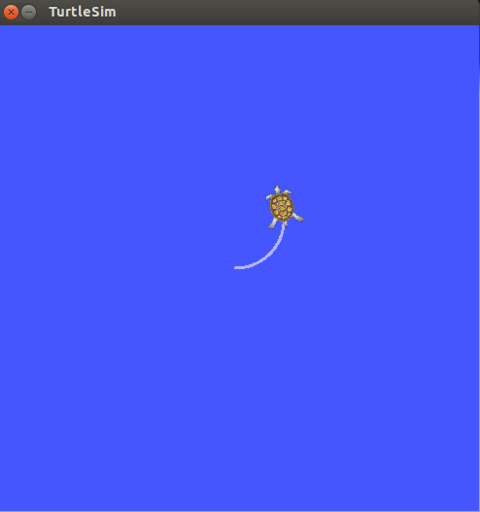
\includegraphics[width=0.7\columnwidth]{pictures/chapter5/rostopic_pub.png}
\caption{발행된 메시지가 반영된 모습}
\end{figure}

\newpage
%-------------------------------------------------------------------------------
\subsection{rosservice : ROS 서비스}\index{rosservice : ROS 서비스}

우선, 서비스(service)\footnote{ROS, rosservice, http://wiki.ros.org/rosservice}에 대해서 이해하고 있어야 한다. 아래 용어정리를 참고하도록 하자. 더 자세한 내용은 섹션~\nameref{sec:RosTerm}(pp.\pageref{def:RosService})에서 설명해두었다. 참고하도록 하자.

\vspace{\baselineskip}
\noindent
\begin{description}
\item[rosservice list] : 활성화된 서비스에 대한 정보를 출력한다
\item[rosservice type 서비스이름] : 서비스 타입을 출력한다
\item[rosservice find 서비스타입] : 지정한 서비스 타입의 서비스를 검색한다
\item[rosservice uri  서비스이름] : ROSRPC uri 서비스를 출력한다
\item[rosservice args 서비스이름] : 서비스 매개변수 출력
\item[rosservice call 서비스이름 매개변수] : 입력된 매개변수로 서비스를 요청한다
\end{description}

\vspace{\baselineskip}
\noindent
※ 아래의 예제를 실행하기 전에 모든 노드를 종료하도록 하자. 그리고 난후, 각각 다른 터미널창에서 아래의 명령어를 실행하여 turtlesim\_node 및 turtle\_teleop\_key를 실행해주자.

\begin{lstlisting}[language=ROS]
roscore
rosrun turtlesim turtlesim_node 
rosrun turtlesim turtle_teleop_key
\end{lstlisting}

\setcounter{num}{0}

\vspace{\baselineskip}
\noindent
\stepcounter{num}\circled{\thenum} rosservice list : 활성화된 서비스에 대한 정보를 출력한다

\begin{lstlisting}[language=ROS]
$ rosservice list
/clear
/kill
/reset
/rosout/get_loggers
/rosout/set_logger_level
/spawn
/teleop_turtle/get_loggers
/teleop_turtle/set_logger_level
/turtle1/set_pen
/turtle1/teleport_absolute
/turtle1/teleport_relative
/turtlesim/get_loggers
/turtlesim/set_logger_level
\end{lstlisting}

\noindent
동일한 네트워크에서 사용중인 서비스가 모두 표시된다.

\vspace{\baselineskip}
\noindent
\stepcounter{num}\circled{\thenum} rosservice type [서비스이름] : 서비스 타입을 출력한다.

\begin{lstlisting}[language=ROS]
$ rosservice type /turtle1/set_pen
turtlesim/SetPen
\end{lstlisting}

\noindent
/turtle1/set\_pen 서비스는 turtlesim/SetPen 형태의 서비스 타입임을 확인할 수 있다.

\vspace{\baselineskip}
\noindent
\stepcounter{num}\circled{\thenum} rosservice find [서비스타입] : 지정한 서비스 타입의 서비스를 검색한다

\begin{lstlisting}[language=ROS]
$ rosservice find turtlesim/SetPen
/turtle1/set_pen
\end{lstlisting}

\noindent
"turtlesim/SetPen" 형태의 서비스 타입의 서비스를 검색하는 명령어이다. 결과로는 "/turtle1/set\_pen" 가 나왔음을 확인할 수 있다.

\vspace{\baselineskip}
\noindent
\stepcounter{num}\circled{\thenum} rosservice uri [서비스이름] : ROSRPC uri 서비스를 출력한다

\begin{lstlisting}[language=ROS]
$ rosservice uri /turtle1/set_pen
rosrpc://192.168.4.185:49714
\end{lstlisting}

\noindent
"/turtle1/set\_pen" 서비스의 ROSRPC uri를 확인할 수 있다.

\vspace{\baselineskip}
\noindent
\stepcounter{num}\circled{\thenum} rosservice args [서비스이름] : 서비스 매개변수 출력

\begin{lstlisting}[language=ROS]
$ rosservice args /turtle1/set_pen
r g b width off
\end{lstlisting}

\noindent
"/turtle1/set\_pen" 서비스의 각 매개변수를 확인할 수 있다. 위의 명령어에서는 r, g, b, width, off 라는 매개변수가 사용됨을 확인할 수 있었다.

\vspace{\baselineskip}
\noindent
\stepcounter{num}\circled{\thenum}  rosservice call [서비스이름] [매개변수] : 입력된 매개변수로 서비스를 요청한다

\begin{lstlisting}[language=ROS]
$ rosservice call /turtle1/set_pen 255 0 0 5 0
\end{lstlisting}

\noindent
"/turtle1/set\_pen" 서비스를 요청하는 명령어이다. 사용된 255 0 0 5 0 은 "/turtle1/set\_pen" 서비스에 사용되는 매개변수(r, g, b, width, off)에 해당되는 수치이다.  빨간색의 r의 최대치인 255으로 하고, g,b 는 모두 0 이므로 펜의 색깔을 빨간색으로 설정하라는 이야기이며, width는 5의 굵기로 설정, off는 0(false)이기에 선이 보이도록 하는것을 의미한다. 그 결과가 아래와 같다. 위 명령어로 서비스를 요청하여 TurtleSim에 사용되는 펜의 특성을 바꾸었고, turtle\_teleop\_key에서 명령을 내려 이동한 결과 아래와 같이 흰색이였던 펜 색이 빨간색으로 표시됨을 확인할 수 있다.

\begin{figure}[h]
\centering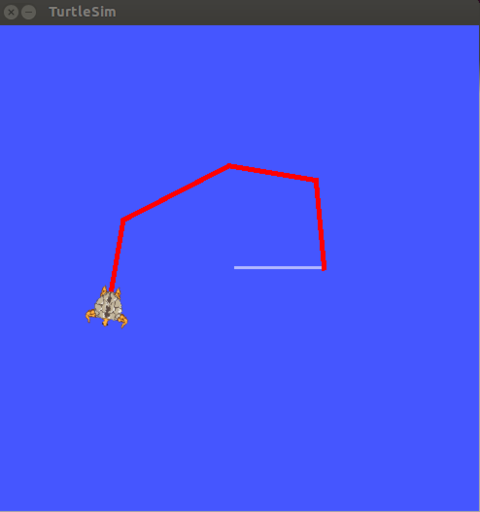
\includegraphics[width=0.5\columnwidth]{pictures/chapter5/rosservice_call.png}
\caption{rosservice call 예제}
\end{figure}

\newpage
%-------------------------------------------------------------------------------
\subsection{rosparam : ROS 매개변수}\index{rosparam : ROS 매개변수}

우선, 매개변수(parameter)\footnote{ROS, rosparam, http://wiki.ros.org/rosparam}에 대해서 이해하고 있어야 한다. 자세한 내용은 섹션~\nameref{sec:RosTerm}(pp.\pageref{def:RosParameter})에서 설명해두었다. 참고하도록 하자.

\vspace{\baselineskip}
\noindent
\begin{description}
\item[rosparam list] : 매개변수 목록 보기
\item[rosparam get 매개변수이름] : 매개변수 값 불러오기
\item[rosparam set 매개변수이름] : 매개변수 값 설정 
\item[rosparam dump 파일이름] : 매개변수를 지정한 파일에 저장한다
\item[rosparam load 파일이름] : 지정한 파일에 저장된 매개변수를 불러온다
\item[rosparam delete 매개변수이름] : 매개변수를 삭제한다 
\end{description}

\vspace{\baselineskip}
\noindent
※ 아래의 예제를 실행하기 전에 모든 노드를 종료하도록 하자. 그리고 난후, 각각 다른 터미널창에서 아래의 명령어를 실행하여 turtlesim\_node 및 turtle\_teleop\_key를 실행해주자.

\begin{lstlisting}[language=ROS]
roscore
rosrun turtlesim turtlesim_node 
rosrun turtlesim turtle_teleop_key
\end{lstlisting}

\setcounter{num}{0}

\noindent
\stepcounter{num}\circled{\thenum} rosparam list : 매개변수 목록 보기

\begin{lstlisting}[language=ROS]
$ rosparam list
/background_b
/background_g
/background_r
/rosdistro
/roslaunch/uris/host_192_168_4_185__39536
/rosversion
/run_id
\end{lstlisting}

\noindent
동일한 네트워크에서 사용중인 매개변수 목록이 표시된다.

\vspace{\baselineskip}
\noindent
\stepcounter{num}\circled{\thenum} rosparam get [매개변수이름] : 매개변수 값 불러오기

\begin{lstlisting}[language=ROS]
$ rosparam get /background_b
255
\end{lstlisting}

\noindent
특정 매개변수 값을 확인하고 싶을때는 위와 같이 "rosparam get" 명령어에 옵션으로 매개변수이름을 적어주면 된다.

\begin{lstlisting}[language=ROS]
$ rosparam get /
background_b: 255
background_g: 86
background_r: 69
rosdistro: 'hydro
  '
roslaunch:
  uris: {host_192_168_4_185__39536: 'http://192.168.4.185:39536/'}
rosversion: '1.9.50
  '
run_id: 93598b26-44f6-11e3-a077-d43d7e970cb0
\end{lstlisting}

\noindent
특정 매개변수가 아니라 모든 매개변수의 값을 확인하고 싶을 경우에는 옵션으로 "/" 를 붙여주면 위와같이 모든 매개변수의 값을 확인할 수 있다.

\vspace{\baselineskip}
\noindent
\stepcounter{num}\circled{\thenum} rosparam set [매개변수이름] : 매개변수 값 설정 

\begin{lstlisting}[language=ROS]
$ rosparam set background_b 0
$ rosservice call clear
\end{lstlisting}

\begin{figure}[h]
\centering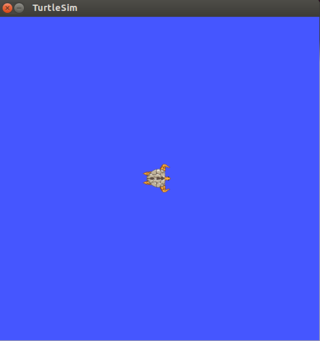
\includegraphics[width=0.4\columnwidth]{pictures/chapter5/rosparam_set1.png}
\centering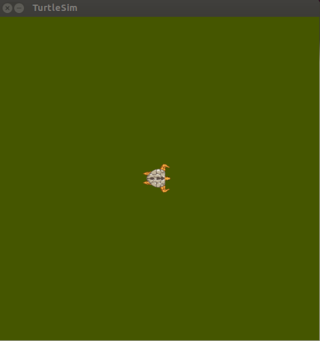
\includegraphics[width=0.4\columnwidth]{pictures/chapter5/rosparam_set2.png}
\caption{rosparam set 예제}
\end{figure}

\noindent
매개변수 값을 설정하는 명령어이다. 위 예제에서 "turtlesim" 노드의 배경색관련 매개변수인 "background\_b" 를 "0"으로 설정하였다. 그러면 rgb 는 255, 86, 69 에서 0, 86, 69 으로 변경되기에 위 오른쪽 그림처럼 짙은 녹색이 된다.

단, "turtlesim" 노드는 매개변수를 매번 읽는 것이 아니기에 "rosparam set background\_b 0" 명령어로 매개변수를 수정후에, "rosservice call clear" 명령어로 화면을 갱신해줘야한다. 이는 노드에 따라 매개변수 반영이 달라지게 된다.

\vspace{\baselineskip}
\noindent
\stepcounter{num}\circled{\thenum} rosparam dump [파일이름] : 매개변수를 지정한 파일에 저장한다

\begin{lstlisting}[language=ROS]
$ rosparam dump ~/parameters.yaml
\end{lstlisting}

\noindent
현재의 매개변수 값을 "parameters.yaml" 라는 파일에 저장하게 된다. 이는 매번 사용되는 매개변수값을 저장하여 다음 실행때에 사용할 수 있어서 매우 편리하다. (~/ 은 유저의 home 폴더를 의미한다)

\vspace{\baselineskip}
\noindent
\stepcounter{num}\circled{\thenum} rosparam delete [매개변수이름] : 매개변수를 삭제한다

\begin{lstlisting}[language=ROS]
$ rosparam delete /background_b
\end{lstlisting}

\noindent
지정한 매개변수를 삭제하는 명령어이다.

\newpage
%-------------------------------------------------------------------------------
\subsection{rosmsg : ROS 메시지 정보}\index{rosmsg : ROS 메시지 정보}

우선, 메시지(message)\footnote{ROS, rosmsg, http://wiki.ros.org/rosmsg}에 대해서 이해하고 있어야 한다. 자세한 내용은 섹션~\nameref{sec:RosTerm}(pp.\pageref{def:RosMessage})에서 설명해두었다. 참고하도록 하자.

\vspace{\baselineskip}
\noindent
\begin{description}
\item[rosmsg list] : 모든 메시지를 목록으로 표시한다
\item[rosmsg show 메시지이름] : 지정한 메시지 정보를 표시한다
\item[rosmsg md5 메시지이름] : md5sum을 표시한다
\item[rosmsg package 패키지이름] : 지정한 패키지에서 사용되는 메시지의 목록을 표시한다
\item[rosmsg packages] : 메시지를 사용하는 모든 패키지의 목록을 표시한다
\end{description}

\vspace{\baselineskip}
\noindent
※ 아래의 예제를 실행하기 전에 모든 노드를 종료하도록 하자. 그리고 난후, 각각 다른 터미널창에서 아래의 명령어를 실행하여 turtlesim\_node 및 turtle\_teleop\_key를 실행해주자.

\begin{lstlisting}[language=ROS]
$ roscore
$ rosrun turtlesim turtlesim_node 
$ rosrun turtlesim turtle_teleop_key
\end{lstlisting}

\setcounter{num}{0}

\vspace{\baselineskip}
\noindent
\stepcounter{num}\circled{\thenum} rosmsg list : 모든 메시지를 목록으로 표시한다

\begin{lstlisting}[language=ROS]
$ rosmsg list
actionlib/TestAction
actionlib/TestActionFeedback
actionlib/TestActionGoal
actionlib/TestActionResult
actionlib/TestFeedback
actionlib/TestGoal
sensor_msgs/Joy
sensor_msgs/JoyFeedback
sensor_msgs/JoyFeedbackArray
sensor_msgs/LaserEcho
zeroconf_msgs/DiscoveredService
...
\end{lstlisting}

\noindent
현재 ROS에 포함되어 있는 패키지에 따라 결과값이 틀려질 수 있다. 이 명령어는 현재 ROS에 설치된 패키지의 모든 메시지를 목록으로 표시하게 된다.

\vspace{\baselineskip}
\noindent
\stepcounter{num}\circled{\thenum} rosmsg show [메시지이름] : 지정한 메시지 정보를 표시한다

\begin{lstlisting}[language=ROS]
$ rosmsg show turtlesim/Pose 
float32 x
float32 y
float32 theta
float32 linear_velocity
float32 angular_velocity
\end{lstlisting}

\noindent
지정한 메시지 정보를 표시한다. 위 예제에서는 "turtlesim/Pose" 라는 이름의 메시지의 정보를 출력해보았다. float32 부동소수점형 변수로 x, y, theta, linear\_velocity, angular\_velocity 의 5개의 정보가 포함되어 있는 메시지임을 확인할 수 있다.

\vspace{\baselineskip}
\noindent
\stepcounter{num}\circled{\thenum} rosmsg md5 [메시지이름] : md5sum\footnote{섹션~\nameref{sec:RosTerm}(pp.\pageref{def:RosMD5})}을 표시한다

\begin{lstlisting}[language=ROS]
$ rosmsg md5 turtlesim/Pose 
863b248d5016ca62ea2e895ae5265cf9
\end{lstlisting}

\noindent
"turtlesim/Pose" 라는 이름의 메시지의 md5 정보를 확인한다. 간혹 메시지 통신중에 MD5 문제가 발생된다면 md5sum 을 확인할 필요가 있는데 이때에 사용되는 명령어이다. 일반적으로 많이 사용되지는 않는다.

\vspace{\baselineskip}
\noindent
\stepcounter{num}\circled{\thenum} rosmsg package [패키지이름] : 지정한 패키지에서 사용되는 메시지의 목록을 표시한다

\begin{lstlisting}[language=ROS]
$ rosmsg package turtlesim 
turtlesim/Color
turtlesim/Pose
\end{lstlisting}

\noindent
특정 패키지에서 사용되는 메시지들을 확인할 수 있다.

\vspace{\baselineskip}
\noindent
\stepcounter{num}\circled{\thenum} rosmsg packages : 메시지를 사용하는 모든 패키지의 목록을 표시한다

\begin{lstlisting}[language=ROS]
$ rosmsg packages
actionlib
actionlib_msgs
actionlib_tutorials
base_local_planner
bond
control_msgs
costmap_2d
\end{lstlisting}

%-------------------------------------------------------------------------------
\subsection{rossrv : ROS 서비스 정보}\index{rossrv : ROS 서비스 정보}

우선, 서비스(service)\footnote{ROS, rosmsg, http://wiki.ros.org/rosmsg}에 대해서 이해하고 있어야 한다. 자세한 내용은 섹션~\nameref{sec:RosTerm}(pp.\pageref{def:RosService})에서 설명해두었다. 참고하도록 하자.

\vspace{\baselineskip}
\noindent
\begin{description}
\item[rossrv list] : 모든 서비스를 목록으로 표시한다
\item[rossrv show 서비스이름] : 지정한 서비스 정보를 표시한다
\item[rossrv md5 서비스이름] : md5sum을 표시한다
\item[rossrv package 패키지이름] : 지정한 패키지에서 사용되는 서비스의 목록을 표시한다
\item[rossrv packages] : 서비스를 사용하는 모든 패키지의 목록을 표시한다
\end{description}

\vspace{\baselineskip}
\noindent
※ 아래의 예제를 실행하기 전에 모든 노드를 종료하도록 하자. 그리고 난후, 각각 다른 터미널창에서 아래의 명령어를 실행하여 turtlesim\_node 및 turtle\_teleop\_key를 실행해주자.

[leftmargin=*]
\begin{lstlisting}[language=ROS]
roscore
rosrun turtlesim turtlesim_node 
rosrun turtlesim turtle_teleop_key
\end{lstlisting}

\setcounter{num}{0}

\vspace{\baselineskip}
\noindent
\stepcounter{num}\circled{\thenum} rossrv list : 모든 서비스를 목록으로 표시한다

\begin{lstlisting}[language=ROS]
$ rossrv list
control_msgs/QueryCalibrationState
control_msgs/QueryTrajectoryState
diagnostic_msgs/SelfTest
dynamic_reconfigure/Reconfigure
gazebo_msgs/ApplyBodyWrench
gazebo_msgs/ApplyJointEffort
gazebo_msgs/BodyRequest
gazebo_msgs/DeleteModel
...
\end{lstlisting}

\noindent
현재 ROS에 포함되어 있는 패키지에 따라 결과값이 틀려질 수 있다. 이 명령어는 현재 ROS에 설치된 패키지의 모든 서비스를 목록으로 표시하게 된다.

\vspace{\baselineskip}
\noindent
\stepcounter{num}\circled{\thenum} rossrv show [서비스이름] : 지정한 서비스 정보를 표시한다

\begin{lstlisting}[language=ROS]
$ rossrv md5 turtlesim/SetPen 
9f452acce566bf0c0954594f69a8e41b
\end{lstlisting}

\noindent
"turtlesim/SetPen" 라는 이름의 서비스의 md5 정보를 확인한다. 간혹 서비스 요청 중에 MD5 문제가 발생된다면 md5sum 을 확인할 필요가 있는데 이때에 사용되는 명령어이다. 일반적으로 많이 사용되지는 않는다.

\vspace{\baselineskip}
\noindent
\stepcounter{num}\circled{\thenum} rossrv package [패키지이름] : 지정한 패키지에서 사용되는 서비스의 목록을 표시한다

\begin{lstlisting}[language=ROS]
$ rossrv package turtlesim 
turtlesim/Kill
turtlesim/SetPen
|turtlesim/Spawn
turtlesim/TeleportAbsolute
turtlesim/TeleportRelative
\end{lstlisting}

\noindent
특정 패키지에서 사용되는 메시지들을 확인할 수 있다.

\vspace{\baselineskip}
\noindent
\stepcounter{num}\circled{\thenum} rossrv packages : 서비스를 사용하는 모든 패키지의 목록을 표시한다

\begin{lstlisting}[language=ROS]
$ rossrv packages
control_msgs
diagnostic_msgs
dynamic_reconfigure
gazebo_msgs
map_msgs
nav_msgs
navfn
nodelet
oroca_ros_tutorials
roscpp
sensor_msgs
std_srvs
tf
tf2_msgs
turtlesim
\end{lstlisting}

%-------------------------------------------------------------------------------
\subsection{rosbag : ROS 로그 정보}\index{rosbag : ROS 로그 정보}
\label{subsub:Rosbag}

우선, 배그(bag)\footnote{ROS, rosbag, http://wiki.ros.org/rosbag}\footnote{ROS, Bags Format, http://wiki.ros.org/Bags/Format}에 대해서 이해하고 있어야 한다. 자세한 내용은 섹션~\nameref{sec:RosTerm}(pp.\pageref{def:RosBag})에서 설명해두었다. 참고하도록 하자.

\vspace{\baselineskip}
\noindent
\begin{description}
\item[rosbag record 옵션 토픽이름] : 지정한 토픽의 메시지를 기록한다
\item[rosbag info bag파일이름] : 배그파일의 정보를 확인한다
\item[rosbag play bag파일이름] : 지정한 배그파일을 재생한다

\item[rosbag compress bag파일이름] : 지정한 배그파일을 압축한다
\item[rosbag decompress bag파일이름] : 지정한 배그파일을 압축해제한다

\item[rosbag filter 입력bag파일 출력bag파일 옵션] : 지정된 내용을 제거한 새로운 bag 파일을 생성한다
\item[rosbag reindex bag파일이름] : 인덱스를 재색인한다

\item[rosbag check bag파일이름] : 지정한 배그파일이 현재 시스템에서 재생 가능한지 확인한다
\item[rosbag fix 입력bag파일 출력bag파일 옵션] : 버전이 다른 재생 불가능 bag파일을 재생가능하게 수정한다
\end{description}

\vspace{\baselineskip}
\noindent
※ 아래의 예제를 실행하기 전에 모든 노드를 종료하도록 하자. 그리고 난후, 각각 다른 터미널창에서 아래의 명령어를 실행하여 turtlesim\_node 및 turtle\_teleop\_key를 실행해주자.

\vspace{\baselineskip}
\begin{lstlisting}[language=ROS]
roscore
rosrun turtlesim turtlesim_node 
rosrun turtlesim turtle_teleop_key
\end{lstlisting}

\setcounter{num}{0}

\noindent
\stepcounter{num}\circled{\thenum} rosbag record [옵션] [토픽이름] : 지정한 토픽의 메시지를 기록한다

\begin{lstlisting}[language=ROS]
$ rostopic list
/rosout
/rosout_agg
/turtle1/cmd_vel
/turtle1/color_sensor
/turtle1/pose
\end{lstlisting}

\noindent
우선, "rostopic list" 명령어를 이용하여 현재 ROS 네트워크에서 사용중인 토픽 목록을 확인한다.

\begin{lstlisting}[language=ROS]
$ rosbag record /turtle1/cmd_vel
[ INFO] [1383546556.032289494]: Subscribing to /turtle1/cmd_vel
[ INFO] [1383546556.035616801]: Recording to 2013-11-04-15-29-16.bag.
\end{lstlisting}

\noindent
사용중인 토픽중에서 기록하고자 하는 토픽을 옵션으로 입력하여 bag기록을 시작한다. 기록을 시작한 후, "turtle\_teleop\_key" 노드에서 키보드로 명령을 내리면서 거북이를 이동시켜본다. 이때에 사용된 "/turtle1/cmd\_vel" 토픽이 기록되게 된다. 기록 종료는 Ctrl + C 으로 종료하면 된다. 위 정보처럼 "2013-11-04-15-29-16.bag" 와 같은 .bag 파일이 생성될 것이다.

\newpage

\begin{figure}[h]
\centering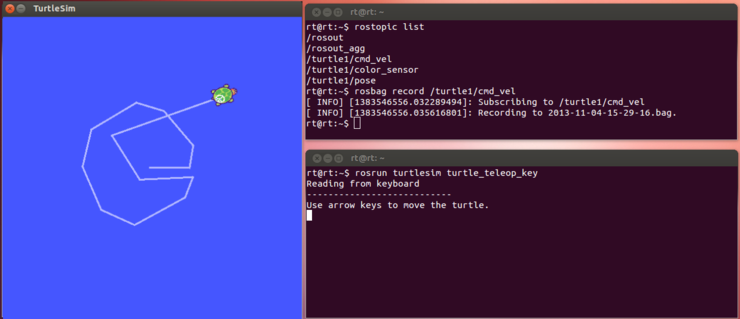
\includegraphics[width=0.8\columnwidth]{pictures/chapter5/rosbag_record.png}
\caption{rosbag record 예제}
\end{figure}

\begin{lstlisting}[language=ROS]
$ rosbag record -a
[ INFO] [1383547478.578148917]: Recording to 2013-11-04-15-44-38.bag.
[ INFO] [1383547479.577915716]: Subscribing to /turtle1/color_sensor
[ INFO] [1383547479.578655855]: Subscribing to /rosout
[ INFO] [1383547479.579363447]: Subscribing to /rosout_agg
[ INFO] [1383547479.579924366]: Subscribing to /turtle1/cmd_vel
[ INFO] [1383547479.580483400]: Subscribing to /turtle1/pose
\end{lstlisting}

\noindent
특정 토픽이 아닌 모든 토픽을 기록하고 싶다면 위와 같이 옵션에 "-a" 를 붙여주면 모든 토픽이 동시에 기록된다.

\vspace{\baselineskip}
\noindent
\stepcounter{num}\circled{\thenum} rosbag info [bag파일이름] : 배그파일의 정보를 확인한다

\begin{lstlisting}[language=ROS]
$ rosbag info 2013-11-04-15-29-16.bag 
path:        2013-11-04-15-29-16.bag
version:     2.0
duration:    16.9s
start:       Nov 04 2013 15:29:19.83 (1383546559.83)
end:         Nov 04 2013 15:29:36.74 (1383546576.74)
size:        23.1 KB
messages:    173
compression: none [1/1 chunks]
types:       geometry_msgs/Twist [9f195f881246fdfa2798d1d3eebca84a]
topics:      /turtle1/cmd_vel   173 msgs    : geometry_msgs/Twist
\end{lstlisting}

\noindent
배그파일의 정보를 확인할 수 있다. 위의 예제에서는 "/turtle1/cmd\_vel" 토픽을 기록하였으며, 총 173개의 메시지가 기록되었다. 사용된 메시지 형태는 "geometry\_msgs/Twist" 이며, 그이외에도 경로, bag 버전, 시간 등의 정보를 확인 할 수 있다.

\vspace{\baselineskip}
\noindent
\stepcounter{num}\circled{\thenum} rosbag play [bag파일이름] : 지정한 배그파일을 재생한다

\begin{lstlisting}[language=ROS]
$ rosbag play 2013-11-04-15-29-16.bag 
[ INFO] [1383548100.180862433]: Opening 2013-11-04-15-29-16.bag

Waiting 0.2 seconds after advertising topics... done.

Hit space to toggle paused, or 's' to step.
[RUNNING]  Bag Time: 1383546576.681423   Duration: 16.855905 / 16.918187     
Done.
\end{lstlisting}

\noindent
기록해둔 "2013-11-04-15-29-16.bag" 를 재생하는 명령어이다. 아래의 그림처럼 원본과 재생시의 데이터가 같음을 확인할 수 있다.

\begin{figure}[h]
\centering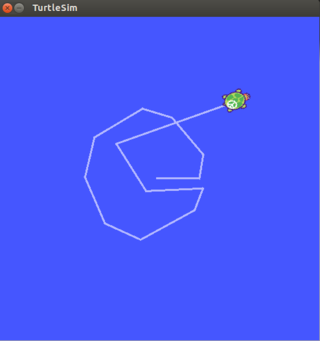
\includegraphics[width=0.4\columnwidth]{pictures/chapter5/rosbag_play1.png}
\centering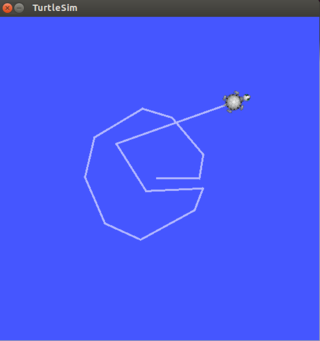
\includegraphics[width=0.4\columnwidth]{pictures/chapter5/rosbag_play2.png}
\caption{rosbag play 예제}
\end{figure}

\vspace{\baselineskip}
\noindent
\stepcounter{num}\circled{\thenum} rosbag compress [bag파일이름] : 지정한 배그파일을 압축한다

\begin{lstlisting}[language=ROS]
$ rosbag compress 2013-11-04-15-29-16.bag 
 2013-11-04-15-29-16.bag                     100%             16.4 KB 00:00  
\end{lstlisting}

\noindent
짧은 시간의 배그파일은 경우에는 그다지 용량이 크지 않아 문제 없지만, 장시간의 데이터를 기록할시에는 저장공간을 많이 차지한다. 위 압축 명령은 이럴때 사용하는 명령어로 압축해놓으면 매우 적은 저장 공간을 차지하게 된다. 위의 예제에서는 아래와 같이 1/3로 축소되었다. 그리고, 압축전 원본 파일은 orig라는 이름이 추가되어 별도로 저장된다.

\vspace{\baselineskip}
\noindent
/home/rt/2013-11-04-15-29-16.bag 8.6kB\\
/home/rt/2013-11-04-15-29-16.orig.bag 23.7kB

\vspace{\baselineskip}
\noindent
\stepcounter{num}\circled{\thenum} rosbag decompress [bag파일이름] : 지정한 배그파일을 압축해제한다

\begin{lstlisting}[language=ROS]
$ rosbag decompress 2013-11-04-15-29-16.bag 
2013-11-04-15-29-16.bag                     100%             16.3 KB 00:00  
\end{lstlisting}

\noindent
압축해제시에는 위의 명령어를 이용하면 된다. 압축전 상태로 원상 복귀된다.


% rosbag filter [입력bag파일] [출력bag파일] [옵션] : 지정된 내용을 제거한 새로운 bag 파일을 생성한다
% rosbag reindex [bag파일이름] : 인덱스를 재색인한다
% rosbag check [bag파일이름] : 지정한 배그파일이 현재 시스템에서 재생 가능한지 확인한다
% rosbag fix [입력bag파일] [출력bag파일] [옵션] : 버전이 다른 재생 불가능 bag파일을 재생가능하게 수정한다

%-------------------------------------------------------------------------------
% -*- root: main.tex -*-
%-------------------------------------------------------------------------------
\chapterimage{chapter_head_6.pdf} 

%-------------------------------------------------------------------------------
\chapter{ROS 도구}

%-------------------------------------------------------------------------------
\section{ROS 도구 (RViz)}\index{ROS 도구 (RViz)}

ROS는 "로봇 운영체제 강좌 : ROS 명령어" 에서 설명한 커맨드형 명령어 이외에도 ROS 활용에 필요한 다양한 도구들이 존재한다. 이는 커맨드형 명령어와 상호보완하는 형태로 ROS 유저들에게는 필수적으로 알아둬야 할 부분이다.

ROS 도구로는 ROS 유저들이 개인적으로 공개한 툴까지 포함하여 상당히 많은 수가 있는데 그 중에서 이번 강좌에서는 1) 3차원 시각화를 돕는 RViz\footnote{ROS wiki, RViz, http://wiki.ros.org/rviz}\footnote{ROS wiki, RViz User Guide, http://wiki.ros.org/rviz/UserGuide}, 2) 데이터 로깅 툴인 rqt\_bag\footnote{ROS wiki, RQT Bag, http://wiki.ros.org/rqt\_bag}, 3) 데이터 플롯 툴인 rqt\_plot\footnote{ROS wiki, RQT Plot, http://wiki.ros.org/rqt\_plot}. 4) 노드간의 관계 및 메시지를 확인 가능한 rqt\_graph\footnote{ROS wiki, RQT Graph, http://wiki.ros.org/rqt\_graph} , 5) GUI 통합 툴인 rqt\footnote{ROS wiki, RQT, http://wiki.ros.org/rqt} 을 알아볼 것이다. 있다. 이들 툴들은 ros와의 직접적인 처리를 행하는 것은 아니지만 ROS를 이용한 프로그래밍에 매우 유용한 보조툴이다. 

특히, ROS Fuerte 버전부터는 RViz는 rqt 라는 이름으로 rqt\_bag, rqt\_plot, rqt\_graph 등과 함께 36가지 플러그인이 통폐합되어 종합 GUI 툴로써 사용 가능해졌다. 그뿐만 아니라 rqt는 QT로 개발되어 있기 때문에 유저들이 자유롭게 플러그인을 개발하여 추가할 수도 있어서 매우 편리하다. 이번 강좌에서는 아래의 내용에 대해서 알아보도록 하자.

\begin{itemize}[leftmargin=*]
\item RViz : 3D visualization tool / 3차원 시각화 툴
\item rqt\_bag : Logging and Visualization Sensor Data, rosbag gui tool / 메시지 기록 GUI 유틸리티
\item rqt\_plot : Data Plot Tool / 2차원 데이터 플롯 툴 
\item rqt\_graph : 노드 및 메시지간의 상관 관계를 그래프로 나타내는 툴
\item rqt : QT 기반의 ROS GUI 개발 툴
\end{itemize}

%-------------------------------------------------------------------------------
\subsection{RViz 개요 및 활용}\index{RViz 개요 및 활용}

RViz는 ROS의 3차원 시각화 툴이다. ROS 네트워크상의 데이터를 3차원으로 표시하는 것이 주요 목적으로 센서 데이터를 시각화하여 확인할 수 있다. 

예를들어, 레이저 레인지 파인더(LRF: Laser Range Finder)의 센서로부터의 장애물과의 거리값, Kinect 및 Xtion과 같은 3차원 거리 센서의 포인트 클라우드 데이터 (PCD: Point Cloud Data), 카메라로부터 취득한 컬러 이미지 값 등을 실시간으로 표시할 수 있다. 

또한, 사용자가 지정한 폴리곤을 이용하여 각종 표시를 지원하고 있다. 특히, Interactive Markers 를 이용하여 사용자 노드로부터의 명령 및 데이터를 수신하여 상호호환적인 움직을 나타낼 수도 있다. 더불어, XML로 URDF(Unified Robot Description Format) 을 작성하여 로봇을 3차원 모델로 표현하고, 각각의 모델은 자유도에 따라 이동 및 구동 가능하도록 할 수 있어서 시뮬레이션 및 실시간 제어에 확인용으로 사용가능하다.

그 이외에 필자가 작성한 패키지중 RViz를 이용하여 표시가능한것을 아래에 링크하였다. 참고하길 바란다.

\begin{figure}[h]
\centering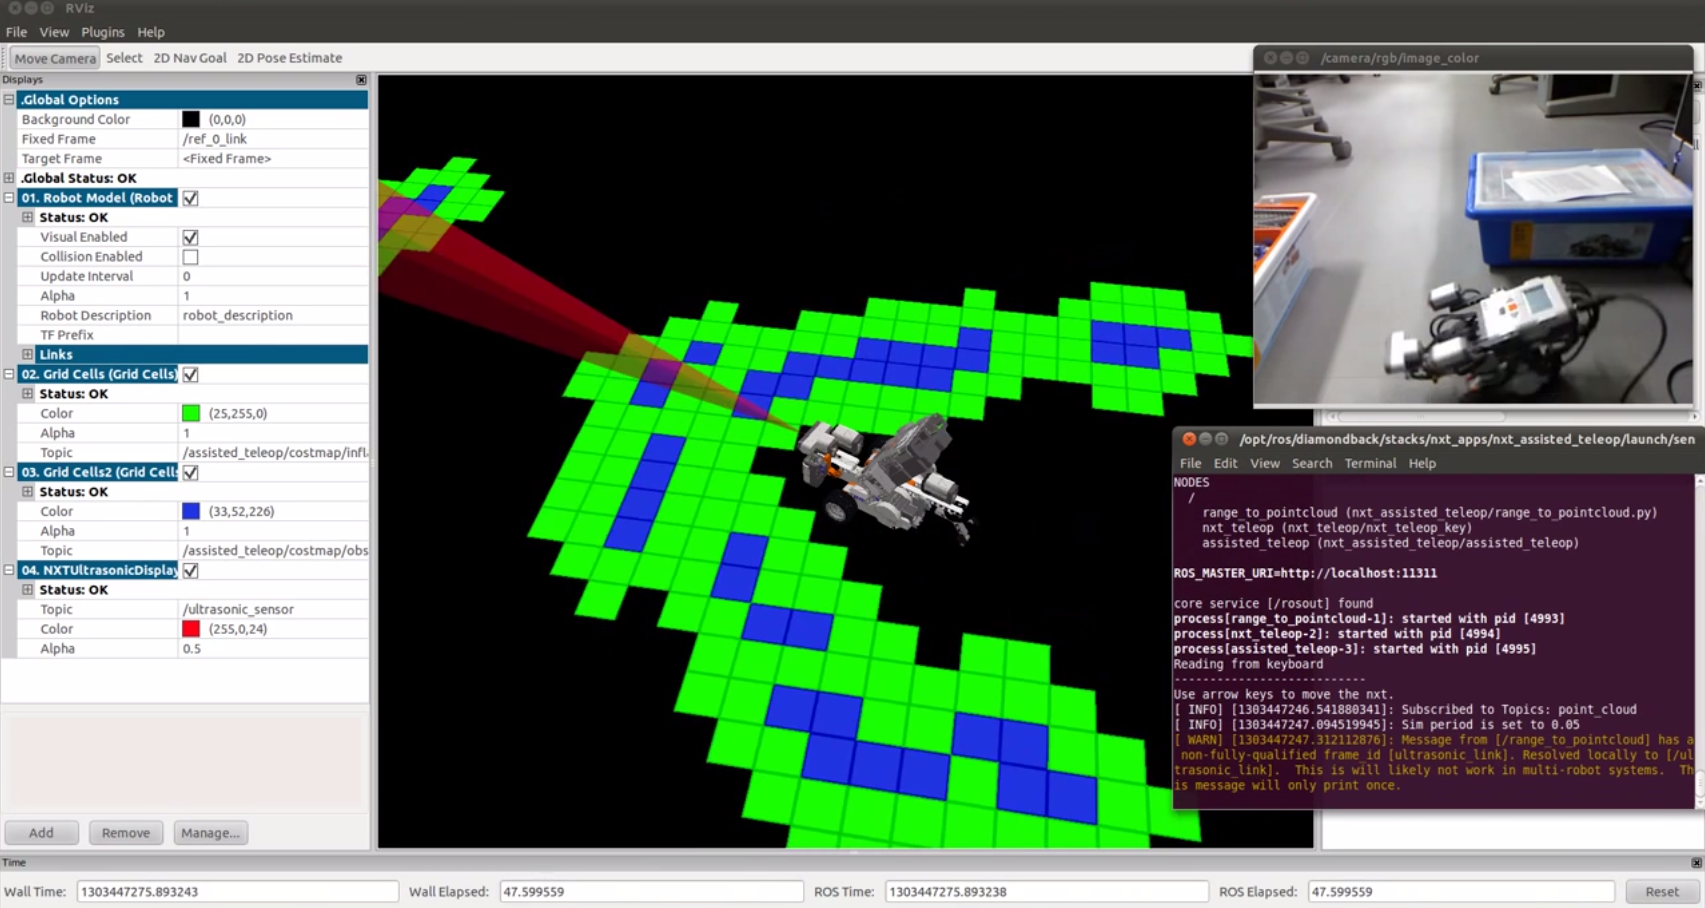
\includegraphics[width=0.7\columnwidth]{pictures/chapter6/rviz_example1.png}
\caption{RViz의 사용예1) 레고를 이용한 모바일 로봇과 초음파 센서를 이용하여 간단한 맵작성}
\end{figure}

\begin{figure}[h]
\centering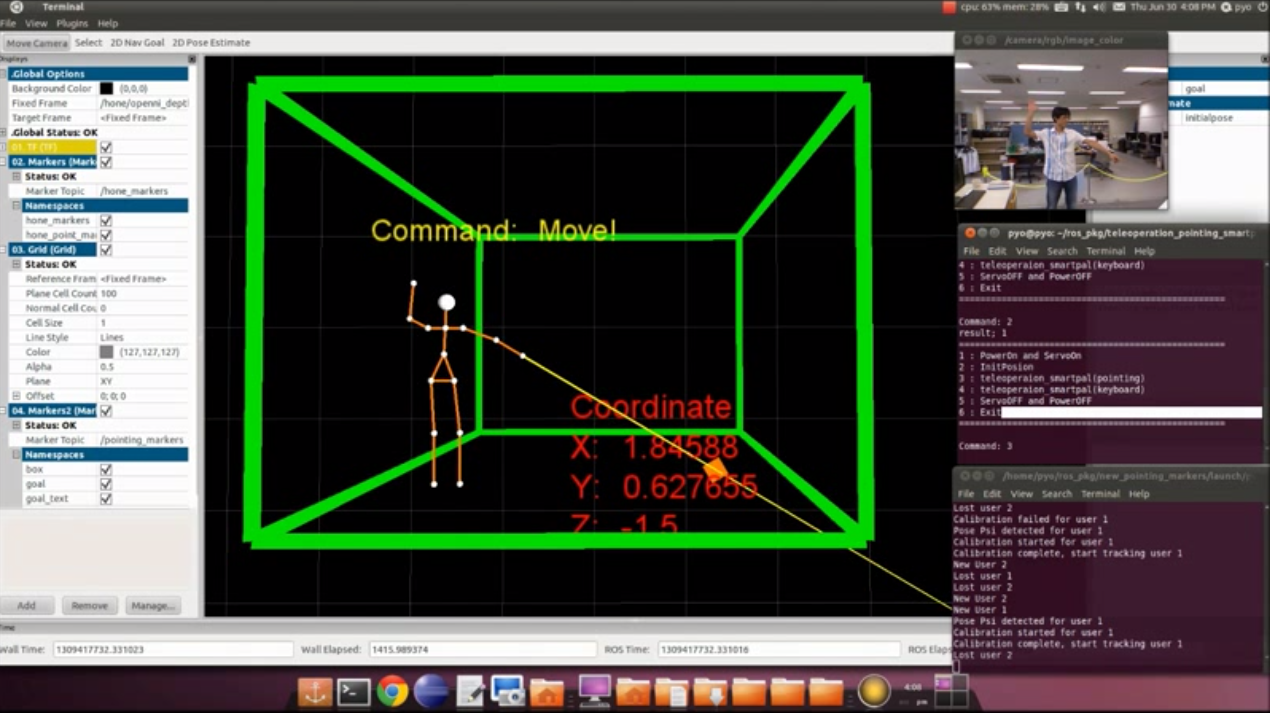
\includegraphics[width=0.7\columnwidth]{pictures/chapter6/rviz_example2.png}
\caption{RViz의 사용예2) 키넥트로부터 사람의 골격을 취득하고 로봇을 제어하는 모습}
\end{figure}

%-------------------------------------------------------------------------------
\subsection{RViz 설치 및 실행}\index{RViz 설치 및 실행}

ROS 설치시에 기본 설치라고도 부를 수 있는 "Desktop-Full Install" 를 설치하게되면 RViz는 기본적으로 설치되어 있다. 만약에 "Desktop-Full Install" 으로 설치하지 않았거나, RViz 가 설치되어 있지 않을 경우에는 아래의 명령어로 설치할 수있다.

\begin{lstlisting}[language=bash]
sudo apt-get install ros-indigo-rviz
\end{lstlisting}

\noindent
RViz 의 실행 명령어는 아래와 같다. (단, roscore 가 실행되어 있어야 한다.)

\begin{lstlisting}[language=bash]
rosrun rviz rviz
\end{lstlisting}

%-------------------------------------------------------------------------------
\subsection{RViz 화면 구성}\index{RViz 화면 구성}

\begin{figure}[h]
\centering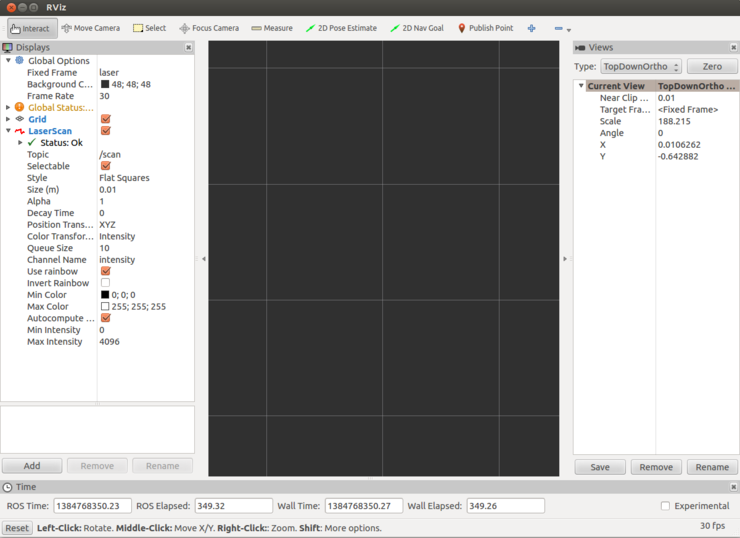
\includegraphics[width=0.8\columnwidth]{pictures/chapter6/rviz.png}
\caption{RViz 화면 구성}
\end{figure}

\begin{enumerate}[leftmargin=*, label=\arabic{*})]
\item 3D 뷰 (3D view)
: 위 화면의 가운데의 검정색 부분을 가르킨다. 각종 데이타를 3차원으로 볼 수 있는 메인 화면이다.

\item 디스플레이(Displays) 
: 왼쪽에 있는 디스플레이 화면은 각종 토픽으로부터 사용자가 원하는 데이타의 뷰를 선택하는 화면이다.

\item 메뉴 (Menu)
: 메뉴는 상단에 놓여져 있다. 현재의 뷰 상태를 저장하거나 읽어오는 명령, 각종 패널의 뷰 옵션을 체크할 수 있다.

\item 툴 (Tools)
: 대부분 네비게이션에 필요한 툴들이 놓여져 있다. 상세한 설명은 네비게이션을 다룰때 설명하도록 하겠다.

\item 뷰 (Views)
: 3D 뷰의 시점을 변경한다.

\item 시간 (Time)
: 현재 시간과 ROS Time 을 실시간으로 보여준다.
\end{enumerate}

%-------------------------------------------------------------------------------
% \subsection{사용 방법}\index{사용 방법}

%-------------------------------------------------------------------------------
\subsection{데이터 표시의 예}\index{데이터 표시의 예}

\begin{figure}[h]
\centering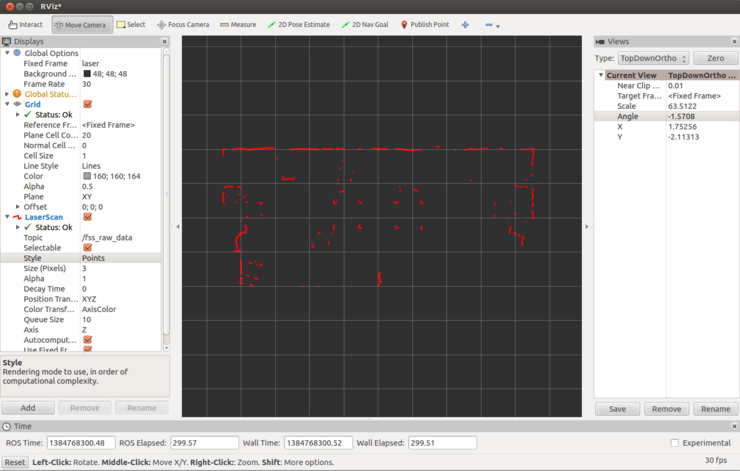
\includegraphics[width=0.7\columnwidth]{pictures/chapter6/rviz_example3.png}
\caption{RViz 사용예3) LRF를 이용한 거리측정}
\end{figure}

\begin{figure}[h]
\centering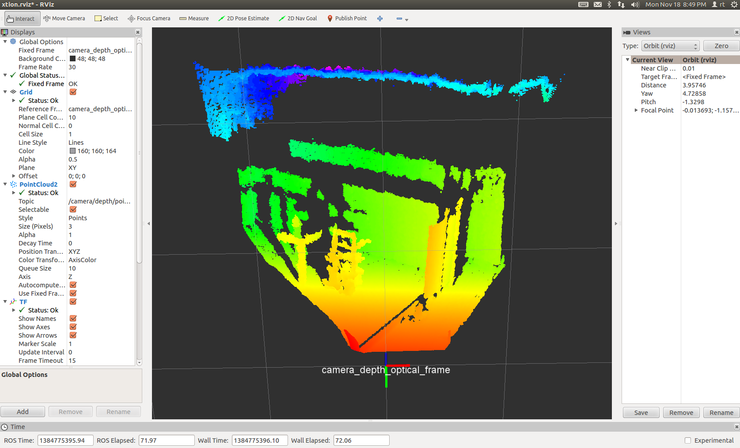
\includegraphics[width=0.7\columnwidth]{pictures/chapter6/rviz_example4.png}
\caption{RViz 사용예4) Xtion 센서로부터 취득한 3차원 거리 값}
\end{figure}

\begin{figure}[h]
\centering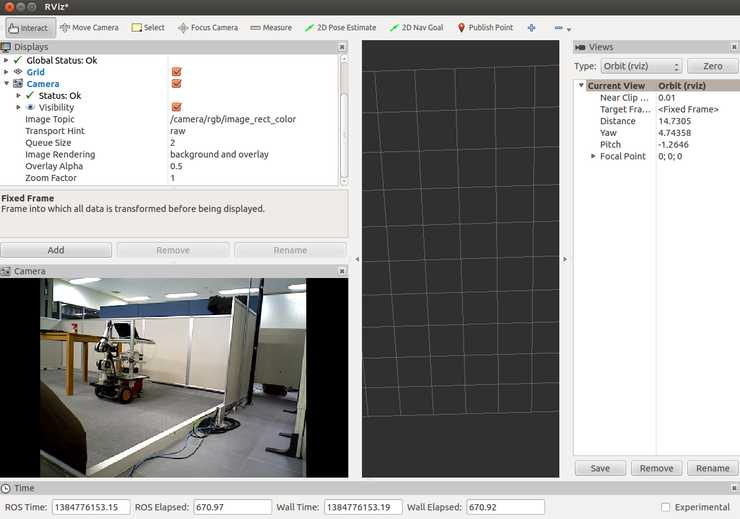
\includegraphics[width=0.7\columnwidth]{pictures/chapter6/rviz_example5.png}
\caption{RViz 사용예5) Xtion 센서에 장착된 카메라를 이용한 이미지 데이터 취득}
\end{figure}

%-------------------------------------------------------------------------------
\section{ROS 도구 (rqt) }\index{ROS 도구 (rqt) }

%-------------------------------------------------------------------------------
\subsection{rqt 개요}\index{rqt 개요}

ROS Fuerte 버전부터는 rqt 라는 이름으로 기존의 rxbag, rxplot, rxgraph 등이 통폐합되어 rqt\_bag, rqt\_plot, rqt\_graph 등을 플러그인으로 하는 종합 GUI 툴로써 사용 가능해졌다. 더불어, rviz 또한 rqt의 플러그인으로 편입되면서 rqt 는 ROS에서 빼놓을 수 없는 중요한 GUI 툴이 되었다. 그뿐만 아니라 rqt는 QT로 개발되어 있기 때문에 유저들이 자유롭게 플러그인을 개발하여 추가할 수도 있어서 매우 편리하다. 이번 강좌에서는 rqt의 대표적인 플러그인인 rqt\_bag, rqt\_plot, rqt\_graph 등 에 대해서 알아보도록 하겠다.

참고로, 그 이외에도 rqt\_action, rqt\_gui, rqt\_plot, rqt\_runtime\_monitorrqt\_bag, rqt\_gui\_cpp, rqt\_pose\_view, rqt\_rvizrqt\_bag\_plugins, rqt\_gui\_py, rqt\_publisher, rqt\_service\_callerrqt\_capabilities, rqt\_image\_view, rqt\_py\_common, rqt\_shellrqt\_console, rqt\_launch, rqt\_py\_console, rqt\_srvrqt\_controller\_manager, rqt\_logger\_level, rqt\_reconfigure, rqt\_tf\_treerqt\_dep, rqt\_moveit, rqt\_robot\_dashboard, rqt\_toprqt\_ez\_publisher, rqt\_msg, rqt\_robot\_monitor, rqt\_topicrqt\_graph, rqt\_nav\_view, rqt\_robot\_steering, rqt\_web 등의 플러그인이 존재한다.\sloppy

%-------------------------------------------------------------------------------
\subsection{rqt 설치}\index{rqt 설치}

ROS 설치시에 기본 설치라고도 부를 수 있는 "Desktop-Full Install" 를 설치하게되면 rqt는 기본적으로 설치되어 있다. 만약에 "Desktop-Full Install" 으로 설치하지 않았거나, rqt 가 설치되어 있지 않을 경우에는 아래의 명령어로 설치할 수있다.

\begin{lstlisting}[language=bash]
sudo apt-get install ros-indigo-rqt ros-indigo-rqt-common-plugins
\end{lstlisting}

추가로, rqt\_graph 에서는 그래프 생성을 위하여 추가적으로 설치해야할 파일이 있다. rqt\_graph 에서는 PyQtGraph, MatPlot, QwtPlot 을 지원하는데 우리는 rqt\_graph 가 추천하는 PyQtGraph 을 사용하도록 하자.

http://www.pyqtgraph.org/downloads/python-pyqtgraph\_0.9.8-1\_all.deb 에서 deb 파일을 받고 클릭하여 설치하도록 하자. 그 뒤 아래와 같이 rqt\_graph를 실행한 후, 프로그램의 오른쪽 상단에 있는 옵션을 의미하는 "기어" 모양의 아이콘을 클릭하면 아래의 첨부 그림과 같이 옵션을 선택할 수 있는데 PyQtGraph 를 선택해주면 된다. PyQtGraph 이외에도 MatPlot, QwtPlot 도 이용 가능하니 원하는 그래프 관련 라이브러리를 이용하면 된다.

\begin{lstlisting}[language=bash]
rqt_graph
\end{lstlisting}

\begin{figure}[h]
\centering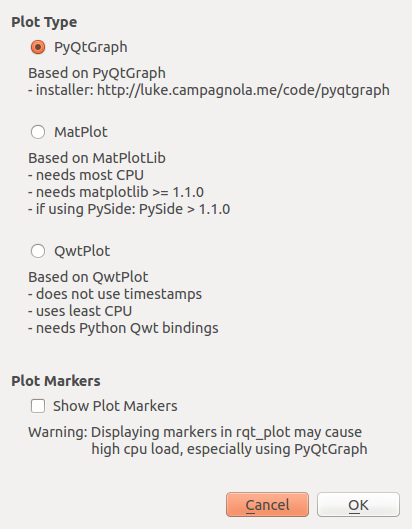
\includegraphics[width=0.5\columnwidth]{pictures/chapter6/rqtplotoption.png}
\caption{rqt\_graph의 설치 옵션}
\end{figure}

%-------------------------------------------------------------------------------
\subsection{rqt 실행 및 각 메뉴 소개}\index{rqt 실행 및 각 메뉴 소개}

실행은 아래와 같다. 단순히 rqt 라고 실행해주면 된다. (정식 실행명령어는 rosrun rqt\_gui rqt\_gui 이다)

\begin{lstlisting}[language=bash]
rqt
\end{lstlisting}

rqt 를 실행해주면 아래와 같이 rqt gui 화면이 나온다.처음 구동하였다면 아무런 표시가 없이 덩그러니 메뉴만 표시된다. 이는 rqt가 직접적으로 수행하는 프로그램인 플러그인이 지정되지 않았기 때문이다. 메뉴를 간단히 설명하자면, File의 경우, 단순히 rqt를 종료하는 서브메뉴만 있다. 플러그인(Plugins) 에는 27가지의 플러그인이 있다. 이를 선택하여 이용하게 된다. 동작(Running) 은 현재 동작중인 플러그인이 표시되어 필요치 않을시에 동작을 중단시킬 수 있는 메뉴이다. 끝으로 시각(Perspectives)은 현재 구동중인 플러그인을 셋트로 다음에도 같은 셋트를 이용하고 싶을때 저장하여 동일한 플러그인들을 실행할때 쓰는 메뉴이다.

\begin{figure}[h]
\centering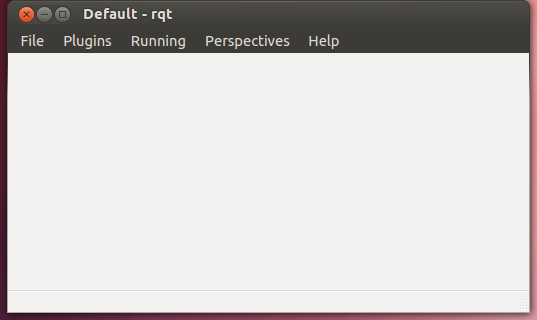
\includegraphics[width=0.6\columnwidth]{pictures/chapter6/rqt.png}
\caption{rqt의 초기 화면}
\end{figure}

%-------------------------------------------------------------------------------
\subsection{rqt 플러그인}\index{rqt 플러그인}

rqt의 상단 메뉴중에서 플러그인(Plugins)\footnote{ROS wiki, Plugins, http://wiki.ros.org/rqt/Plugins}\footnote{ROS wiki, RQT Common Plugins, http://wiki.ros.org/rqt\_common\_plugins}을 선택하면 27가지의 플러그인을 확인할 수 있다. 이 플러그인은 아래의 역할을 담당한다. 대부분 매우 필요한 기능등을 갖춘 rqt 의 기본 플러그인이다. 필요에 의해서 사용자가 개발한 플러그인도 추가 가능하다.

\subsubsection{액션 (Action)}
Action Type Browser | Action 타입의 데이터 구조를 확인하는 플러그인 
\subsubsection{구성 (Configuration)}
Dynamic Reconfigure | 노드들에서 제공하는 설정값 변경을 위한 GUI 설정값 변경 플러그인\\
Launch | roslaunch 의 GUI 플러그인, 로스런치의 이름 및 구성이 생각안날때 매우 유용하다.\\
\subsubsection{내성 (Introspection)}
Node Graph | 구동중인 모든 노드들의 관계도 및 메시지의 흐름을 확인할 수 있는 그래프 뷰 형식의 플러그인\\
Package Graph | 노드의 의존 관계를 표시하는 그래프 뷰 형식의 플러그인\\
Process Monitor | 현재 실행중인 노드들의 CPU사용률, 메모리사용륭, 스레드수 등을 확인 가능하다.\\
\subsubsection{로깅 (Logging)}
Bag | ROS 데이터 로깅 관련 플러그인\\
Console | 노드들에서 발생되는 경고(Warning), 에러(Error) 등의 메시지들을 한 화면에서 확인 가능한 플러그인\\
Logger Level | ROS의 Debug, Info, Warn, Error, Fatal 로거 정보를 선택하여 표시할 수 있는 GUI 툴\\
\subsubsection{다양한 툴 (Miscellaneous Tools)}
Python Console | 파이썬 콘솔 화면 플러그인\\
Shell | 쉘(shell)을 구동하는 플러그인\\
Web | 웹 브라우저를 구동하는 플러그인\\
\subsubsection{로봇 (Robot)}
사용하는 로봇에 따라 계기판(dashboard) 등의 플러그인을 이곳에 추가하면 된다. \\
\subsubsection{로봇툴 (Robot Tools)}
Controller Manager | 컨트롤러 제어에 필요한 플로그인\\
Diagnostic Viewer | 로봇 디바이스 및 에러 확인 플러그인\\
Moveit! Monitor | 로봇 팔 계획에 사용되는 Moveit! 데이터를 확인하는 플러그인\\
Robot Steering | 로봇 조정 GUI 툴, 원격 조정에서 이 GUI 툴을 이용하여 로봇 조종하기에 유용함.\\
Runtime Monitor | 실시간으로 노드들에서 발생되는 에러 및 경고를 확인가능한 플러그인\\
\subsubsection{서비스 (Services)}
Service Caller | 구동중인 서비스 서버에 접속하여 서비스를 요청하는 GUI 플러그인, 서비스 테스트에 유용하다.\\
Service Type Browser | 서비스 타입의 데이터 구조를 확인하는 플러그인\\
\subsubsection{토픽 (Topics)}
Easy Message Publisher | 토픽을 GUI 환경에서 발행가능 한 플러그인\\
Topic Publisher | 토픽을 생성하여 발행가능한 GUI 플러그인, 토픽 테스트에 매우 유용하다.\\
Topic Type Browser | 토픽 타입의 데이터 구조 확인 플러그인, 토픽 타입 확인에 매우 유용하다.\\
Topic Monitor | 현재 사용중인 토픽을 나열, 그 중에서 사용자가 선택한 토픽의 정보를 확인하는 플러그인\\
\subsubsection{시각화 (Visualization)}
Image View | 카메라의 영상 데이터를 확인 가능한 플러그인, 간단한 카메라 데이터 테스트에 유용하다.\\
Navigation Viewer | 로봇 네비게이션의 위치 및 목표지점 확인하는 플러그인\\
Plot | 2차원 데이터 플롯 GUI 플러그인, 2차원 데이터의 도식화에 매우 유용하다.\\
Pose View | 현재 tf의 위치 및 모델의 위치 표시 플러그인\\
RViz | 3차원 시각화 툴인 RViz 플러그인\\
TF Tree | tf 관계를 트리로 나타내는 그래프 뷰 형식의 플러그인\\

\begin{figure}[h]
\centering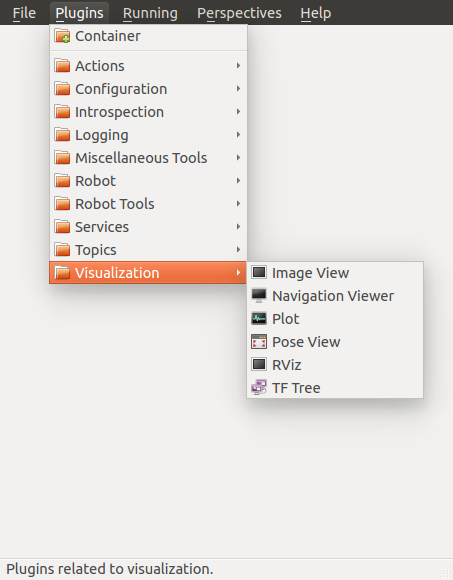
\includegraphics[width=0.8\columnwidth]{pictures/chapter6/rqt_plugin.png}
\caption{rqt 플러그인}
\end{figure}

\vspace{\baselineskip}
\noindent
이 들의 모든 플러그인을 설명하기 어렵고, 이번 강좌에서는 가장 빈번히 사용되는 rqt\_bag, rqt\_graph, rqt\_plot 등 에대해서 알아보도록 하겠다.

%-------------------------------------------------------------------------------
\subsection{rqt\_plot}\index{rqt\_plot}

rqt\_plot 은 2차원 데이터 플롯 툴이다. 플롯이라하면 좌료를 그리다라는 의미이다. 즉, ROS 메시지를 받아서 이를 좌표에 뿌리게 되는 것을 의미한다. 예를들어 turtlesim 노드 pose 메시지의 x 좌표와  y좌표를 좌표에 표기해보도록 하자. 우선, turtlesim 패키지의 turtlesim\_node 을 구동하자.

\begin{lstlisting}[language=ros]
$ rosrun turtlesim turtlesim_node 
\end{lstlisting}

다음으로, rqt\_plot 을 아래의 조건으로 구동하여 좌표를 작성한다. (원래는 rqt 를 구동후에 Plot 플러그인을 불러와서 GUI환경에서 토픽을 설정하면 되야하지만, 현재 버전에서는 이상하게 구동하지 않는다. 그러므로 아래의 명령어로 대채하여 설명한다.)

\begin{lstlisting}[language=ros]
rqt_plot /turtle1/pose/
\end{lstlisting}

다음으로, turtlesim 패키지의 turtle\_teleop\_key 을 구동하여, 화면속의 거북이를 이리저리 움직여보자.

\begin{lstlisting}[language=ros]
$ rosrun turtlesim turtle_teleop_key
\end{lstlisting}

그러면 빨간색 선이 거북이의 x위치가 x 좌표, 파란선이 거북이의 y위치가 y좌표에 표시됨을 확인할 수 있을 것이다. 이와 같이 2차원 데이터의 좌표 표시에 매우 유용한 툴로 지금은 turtlesim 을 이용하였지만, 사용자가 개발한 노드의 2차원 데이터 표시에 매우 유용할 것이다. 특히, 센서값 표시에 적합하다.

\begin{figure}[h]
\centering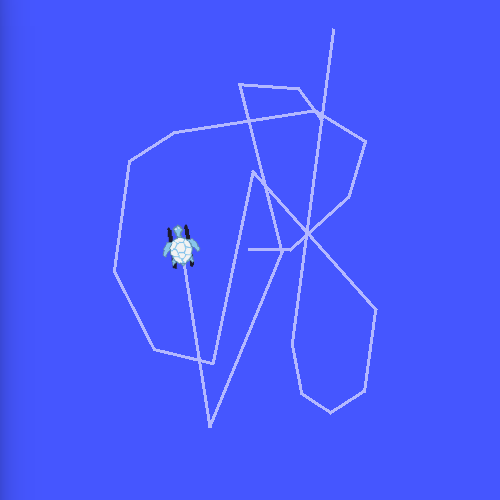
\includegraphics[height=50mm]{pictures/chapter6/turtlesim_rqt_plot1.png}
\centering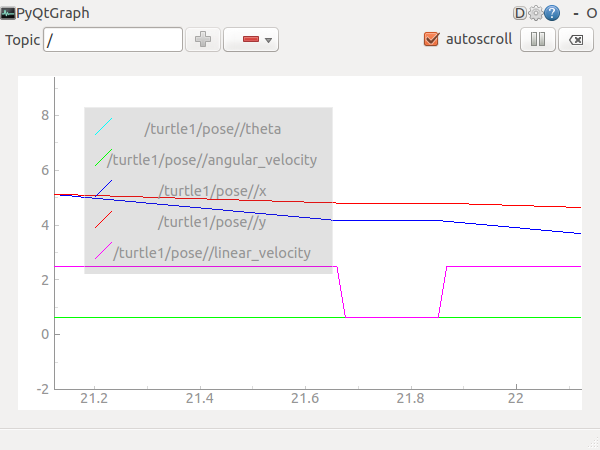
\includegraphics[height=50mm]{pictures/chapter6/turtlesim_rqt_plot2.png}
\caption{rqt\_plot 예제}
\end{figure}

%-------------------------------------------------------------------------------
\subsection{rqt\_bag}\index{rqt\_bag}

메시지 기록을 시각화한 GUI 툴이다. "로봇 운영체제 강좌 : ROS 정보 명령어 (rosbag)" 에서 다룬 내용을 시각화하면 편집 가능한 툴로 이미지 값등과 함께 편집할 때 매우 유용한 툴이다.

이를 테스트하기 위해서 위헤서 다룬 rqt\_graph 및 Image View 에서 다룬 turtlesim 및 uvc camera 관련의 노드들을 전부 실행해 주자. 그 뒤, 아래의 명령어로 카메라의 "/image\_raw" 와 터틀시뮬레이션의 "/turtle1/cmd\_vel" 값을 bag 파일로 생성하자.

\begin{lstlisting}[language=ros]
$ rosbag record /image_raw /turtle1/cmd_vel
\end{lstlisting}

그 후, 아래의 명령어로 rqt를 구동 후, 플러그인(Plugins) 메뉴에서 Bag를 선택한다. 그 뒤 왼쪽 상단의 폴더 모양(Load Bag)의 아이콘을 선택하여 방금전에 기록해둔 *.bag 파일을 불러오도록 하자. 그러면 아래의 화면처럼 영상 및 cmd\_vel 값을 확인할 수 있다. 또한, 이를 확대, 재생, 시간별 데이터 수 등을 확인할 수 있으며, 오른쪽 마우스를 누르면 Publish 라는 옵션이 있는데 이를 통해 메시지를 다시 발행할 수도 있다.

\begin{lstlisting}[language=ros]
$ rqt
\end{lstlisting}

\begin{figure}[h]
\centering\includegraphics[width=0.9\columnwidth]{pictures/chapter6/rqt_bag.png}
\caption{rqtbag 예제}
\end{figure}

%-------------------------------------------------------------------------------
\subsection{rqt\_graph}\index{rqt\_graph}

현재 구동중인 노드 및 ROS 네트워크상에 전송되고 있는 메시지간의 상관 관계를 그래프로 나타내주는 툴이다. 현재 ROS 네트워크의 상황을 파악하는데에 매우 유용하다.

사용방법은 매우 간단한다. 아래의 명령어로 rqt를 구동후, 플러그인(Plugins) 메뉴에서 ROS Graph를 선택하면 그것으로 끝이다. 현재, 카메라 및 터틀봇시뮬레이션을 구동하셨을때의 노드 및 메시지의 상황은 아래 그림처럼 나타난다.

\begin{lstlisting}[language=ros]
$ rqt
\end{lstlisting}

\begin{figure}[h]
\centering\includegraphics[width=0.9\columnwidth]{pictures/chapter6/rqt_graph.png}
\caption{rqt\_graph 예제}
\end{figure}

%-------------------------------------------------------------------------------
\subsection{Image View}\index{Image View}

카메라의 이미지 데이터를 표시하는 플러그인이다. 이미지 처리 프로세스는 아니지만, 단순히 영상을 확인하는 용도로는 매우 간단하기에 유용하다.

일반 USB CAM의 경우, UVC을 지원하기에 ROS의 "uvc\_camera"\footnote{ROS wiki, UVC Camera, http://wiki.ros.org/uvc\_camera} 패키지를 이용하면 된다. 우선, 아래의 명령어로 "uvc\_camera" 패키지를 설치하도록 하자.

\begin{lstlisting}[language=ROS]
$ sudo apt-get install ros-indigo-uvc-camera 
\end{lstlisting}

USB CAM을 컴퓨터의 USB에 연결하고, 아래의 명령어로 uvc\_camera 패키지의 uvc\_camera\_node 노드를 구동하자.

\begin{lstlisting}[language=ros]
$ rosrun uvc_camera uvc_camera_node
\end{lstlisting}

그 후, 아래의 명령어로 rqt를 구동후, 플러그인(Plugins) 메뉴에서 이미지 뷰(Image View)를 선택한다. 그 뒤 왼쪽 상단의 메시지 선택란을 "/image\_raw"를 선택하면 아래의 화면처럼 영상을 확인할 수 있다. 

\begin{lstlisting}[language=ros]
$ rqt
\end{lstlisting}

이상으로 rqt 를 대략적인 개요, 설치, 사용 방법에 대해서 설명하였다. 이 강좌를 통해서 모든 플러그인의 설명을 하는 것을 불가능했지만 위에서 설명한 몇가지 예를 기반으로 직접 사용해보기를 추천한다. ROS 노드와 같은 직접적으로 로봇 및 센서 처리에 관련한 내용은 아니지만, 이와 같은 작업들을 수행하는데 있어서 데이터를 저장, 보존, 수정, 현황파악 등에 도움이 되는 보조툴로서 사용가능하다. 













%-------------------------------------------------------------------------------
% -*- root: main.tex -*-
%-------------------------------------------------------------------------------
\chapterimage{chapter_head_7.pdf} 

%-------------------------------------------------------------------------------
\chapter{ROS 기본 프로그래밍}
\label{cha:RosPrograming}

%-------------------------------------------------------------------------------
\section{메시지, 토픽, 서비스, 매개변수}\index{메시지, 토픽, 서비스, 매개변수}

%-------------------------------------------------------------------------------
\subsection{ROS 메시지 통신}\index{ROS 메시지 통신}

이전 챕터 내용들이 ROS 개론을 설명하였다면 이번 부터가 본격적인 ROS 프로그래밍이라고 볼 수 있다. 이전 내용에서 제일 많이 나온 단어라고 치면 "메시지, 토픽, 서비스, 매개변수" 가 가장 빈번히 언급되었다. 그도 그럴것이, 메시지, 토픽, 서비스, 매개변수는 ROS 에서 가장 핵심 부분이라고 할 수 있다. 각기 목적에 따라 분화된 최소 실행 단위인 노드들은 메시지 통신을 통해 노드간의 입/출력 데이터를 주고 받는 처리를 하고 있다.

\begin{definition*}[메시지(message,msg)]
노드는 메시지를 통해 노드간의 데이터를 주고받게 된다. 메시지는 integer, floating point, boolean 와 같은 변수형태이다. 또한, 메시지안에 메시지를 품고 있는 간단한 데이터 구조 및 메시지들의 배열과 같은 구조도 사용할 수 있다. 

메세지를 이용한 통신방법으로는 TCPROS, UDPROS 방식등이 있으며, 단방향 메시지 송/수신 방식의 토픽과 양방향 메시지 요청/응답 방식의 서비스를 이용하고 있다.
\end{definition*}

메시지 통신을 하나의 그림으로 설명하면 아래와 같다고 볼 수 있다. 작은 목적 단위로 세분화된 실제 처리 프로그램인 노드는 다른 노드와의 데이터 송수신에 메시지 통신 방법을 이용하고 있다. 이 메시지 통신에는 크게 토픽과 서비스로 나뉘고 큰 틀에서는 매개변수 또한 메시지 통신이라고 볼 수있다. 이 세가지 메시지 통신방식인 토픽, 서비스, 매개변수를 이번 강좌에서 소개하고 각각의 특징을 ROS 프로그램 작성전에 미리 익혀두고자 한다. 그 후, 이어지는 강좌들에서 실전을 통해 자세히 다룰 예정이다.

\begin{figure}[h]
\centering\includegraphics[width=0.5\columnwidth]{pictures/chapter7/msgtrans1.png}
\caption{메시지 통신 상관 관계}
\end{figure}

%-------------------------------------------------------------------------------
\subsection{토픽 (topic)}\index{토픽 (topic)}

\begin{center} 
토픽(topic)은 \textbf{이야깃거리}이다.\\ 
\end{center}

발행자 노드가 하나의 이야깃거리에서 대해서 토픽이라는 이름으로 마스터에 등록한 후, 이야깃거리에 대한 이야기를 메시지 형태로 발행한다. 이 이야깃거리를 수신 받기를 원하는 구독자 노드는 마스터에 등록된 토픽의 이름에 해당되는 발행자 노드의 정보를 받는다. 이 정보를 기반으로 구독자 노드는 발행자 노드와 직접적으로 연결하여 메시지를 송/수신 받게 된다. \\

이를 나타낸 그림이 아래와 같다. 단방향 통신이기에 센서가 취득한 정보를 단순히 전달하는 용도로 많이 사용되는 메시지 통신 방식이다.

\begin{figure}[h]
\centering\includegraphics[width=0.7\columnwidth]{pictures/chapter7/msgtrans2.jpg}
\caption{토픽}
\end{figure}

%-------------------------------------------------------------------------------
\subsection{서비스(service)}\index{서비스(service)}

발행과 구독 개념의 토픽 통신 방식은 비동기 방식이라 필요에 따라서 주어진 데이터를 전송하고 받기에 매우 훌륭한 방법이다. 또한, 한번의 접속으로 지속적인 메시지를 송/수신하기 때문에 지속적으로 메시지를 발송해야하는 센서 데이터에 적합하여 많이 사용되고 있다. 

하지만, 경우에 따라서는 요청과 응답이 함께 사용되는 동기 방식의 메시지 교환 방식도 필요하다. 이에 따라, ROS에서는 서비스라는 이름으로 메시지 동기 방식을 제공하고 있다. 

서비스는 요청이 있을 경우에 응답을 하는 서비스 서버와 요청을 하고 응답을 받는 서비스 클라이언트로 나뉘어 있다. 서비스는 토픽과는 달리 1회성 메시지 통신이다. 서비스의 요청과 응답이 완료되면 연결된 두 노드의 접속은 끊기게 된다. 

이러한 서비스는 로봇에게 특정의 일을 수행하는 요청시에 명령어로써 많이 사용된다. 혹은, 특정 조건에 의해 이벤트를 발생해야할 노드에 사용되는 경우가 많다. 1회성 메시지 이기에 네트워크에 부하가 적다는 이유로 토픽을 대체하는 수단으로도 사용되는 등 매우 유용한 통신 수단이다.

\begin{figure}[h]
\centering\includegraphics[width=0.7\columnwidth]{pictures/chapter7/msgtrans3.png}
\caption{서비스}
\end{figure}

%-------------------------------------------------------------------------------
\subsection{매개변수(parameter)}\index{매개변수(parameter)}

노드에서 사용되는 매개변수를 말한다. 흔히, 윈도우즈 프로그램에서 *.ini 설정파일과 같다고 생각하면 된다. 디폴트로 설정 값들이 지정되어 있고, 필요에 의해서 외부에서 이 매개변수를 읽기, 쓰기가 가능하다. 특히, 상황에 맞추어 이 매개변수를 외부에서 쓰기기능을 이용하여 설정값을 실시간으로 바꿀수 있기에 매우 유용한 방법이다. 이는 엄밀히 따지면, 메시지 통신이라고 볼 수 없지만, 필자는 메시지를 이용한다는 점에서 메시지 통신의 범위에 속한다고 본다. 사용 예를 들자면 접속하는 USB포트 및 카메라 캘리브레이션 값, 속도 및 명령어들의 최대/최저 값 등의 설정 등을 꼽을 수 있다.

\begin{figure}[h]
\centering\includegraphics[width=0.6\columnwidth]{pictures/chapter7/msgtrans4.png}
\caption{매개변수}
\end{figure}

%-------------------------------------------------------------------------------
\section{메시지 발행자 노드와 구독자 노드 작성 및 실행}\index{메시지 발행자 노드와 구독자 노드 작성 및 실행}

%-------------------------------------------------------------------------------
\subsection{목적}

ROS 메시지 통신에서 사용되는 발행자(Publisher) 와 구독자(Subscriber) 라는 용어는 쉽게 우리말로 따지면 송신과 수신역할을 담당하게 된다. ROS에서는 송신측을 Publisher, 수신측을 Subscriber 라고 부르고 있다. 이 강좌에서는 간단한 메시지 파일을 작성해보고, 발행자(Publisher) 노드 와 구독자(Subscriber) 노드를 작성 및 실행하는 것을 목적으로 한다.

%-------------------------------------------------------------------------------
\subsection{패키지 생성}

아래의 명령어는 "oroca\_ros\_tutorials" 라는 패키지를 생성하는 명령어이다. 이 패키지는 의존하는 패키지로 "std\_msgs"와 "roscpp"를 옵션으로 달아주었다. ROS의 표준 메시지 패키지인 std\_msgs 와 ROS에서 c/c++을 사용하기 위하여 클라이언트라이브러인 roscpp를 사용하겠다는 것으로 패키지 생성에 앞어서 미리 설치해야한다는 의미이다. 이러한 의존하는 패키지의 설정은 패키지 생성할 때 지정할 수도 있지만, 생성 후 package.xml 에서 직접 입력하여도 된다.

\begin{lstlisting}[language=ROS]
$ cd ~/catkin_ws/src
$ catkin_create_pkg oroca_ros_tutorials std_msgs roscpp
\end{lstlisting}

위와 같이 패키지를 생성하였으면 "\textasciitilde/catkin\_ws/src"에 "oroca\_ros\_tutorials" 라는 패키지 폴더 및 ROS 패키지가 갖추어야할 기본 내부 폴더 및 CMakeLists.txt 와 package.xml가 생성된다. 다음은 아래와 같이 ls 명령어를 입력하여 내용을 보던가 윈도우의 탐색기와 같은 역할을 하는 GUI기반의 Nautilus를 이용하여 패키지 내부를 살펴보도록 하자.

\begin{lstlisting}[language=ROS]
$ ls
include       %*.......... 인클루드 폴더*)
src           %*.......... 소스코드 폴더*)
CMakeLists.txt%*.......... 빌드 설정 파일*)
\end{lstlisting}

%-------------------------------------------------------------------------------
\subsection{패키지 설정 파일 (package.xml) 수정}

ROS의 필수 설정 파일 중 하나인 package.xml 은 패키지 정보를 담은 XML 파일로써 패키지의 이름, 저작자, 라이선스, 의존성 패키지 등을 기술하고 있다. 아래의 명령어로 gedit 툴을 이용하여 파일을 열고 현재의 노드에 맞도록 수정해보자.

\begin{lstlisting}[language=ROS]
$ gedit package.xml 
\end{lstlisting}

아래의 코드는 package.xml 를 이번 노드에 맞도록 수정한 내용이다. 내용중에 필자의 개인 정보가 포함되어 있으니, 이를 자신에 맞게 수정해주길 바란다. 각 옵션의 세부 설명은 섹션~\ref{sec:RosBuildSystem}~\nameref{sec:RosBuildSystem}(pp.\pageref{sec:RosBuildSystem})를 참고하길 바란다.

\begin{lstlisting}[language=XML]
<?xml version="1.0"?>
<package>
  <name>oroca_ros_tutorials</name>
  <version>0.1.0</version>
  <description>The oroca_ros_tutorials package</description>

  <maintainer email="passionvirus@gmail.com">Yoonseok Pyo</maintainer>
  <url type="website">http://oroca.org</url>
  <url type="repository">https://github.com/oroca/oroca_ros_tutorials.git</url>
  <author email="passionvirus@gmail.com">Yoonseok Pyo</author>

  <license>MIT</license>

  <buildtool_depend>catkin</buildtool_depend>

  <build_depend>roscpp</build_depend>
  <build_depend>std_msgs</build_depend>
  <build_depend>message_generation</build_depend>

  <run_depend>roscpp</run_depend>
  <run_depend>std_msgs</run_depend>
  <run_depend>message_runtime</run_depend>

  <export>
  </export>
</package>
\end{lstlisting}

%-------------------------------------------------------------------------------
\subsection{빌드 설정 파일 (CMakeLists.txt) 수정}

ROS의 빌드 시스템인 캐킨(cakin)은 기본적으로 CMake를 이용하고 있어서 패키지 폴더에 CMakeLists.txt 라는 파일에 빌드 환경을 기술하고 있다. 이는 실행 파일 생성, 의존성 패키지 우선 빌드, 링크 생성 등을 설정하게 되어 있다.

\begin{lstlisting}[language=ROS]
$ gedit CMakeLists.txt 
\end{lstlisting}

아래의 코드는 CMakeLists.txt 를 이번 노드에 맞도록 수정한 내용이다.

\begin{lstlisting}[language=make]
cmake_minimum_required(VERSION 2.8.3)
project(oroca_ros_tutorials)

## Find catkin and any catkin packages
find_package(catkin REQUIRED COMPONENTS roscpp std_msgs message_generation)

## Declare ROS messages and services
add_message_files(FILES msgTutorial.msg)

## Generate added messages and services
generate_messages(DEPENDENCIES std_msgs)

## Declare a catkin package
catkin_package(
  #INCLUDE_DIRS include
  LIBRARIES oroca_ros_tutorials
  CATKIN_DEPENDS roscpp std_msgs
  DEPENDS system_lib
)

## Build node
include_directories(include ${catkin_INCLUDE_DIRS})

add_executable(ros_tutorial_msg_publisher src/ros_tutorial_msg_publisher.cpp)
target_link_libraries(ros_tutorial_msg_publisher ${catkin_LIBRARIES})
add_dependencies(ros_tutorial_msg_publisher oroca_ros_tutorials_generate_messages_cpp)

add_executable(ros_tutorial_msg_subscriber src/ros_tutorial_msg_subscriber.cpp)
target_link_libraries(ros_tutorial_msg_subscriber ${catkin_LIBRARIES})
add_dependencies(ros_tutorial_msg_subscriber oroca_ros_tutorials_generate_messages_cpp)
\end{lstlisting}

%-------------------------------------------------------------------------------
\subsection{메시지 파일 작성}

CMakeLists.txt 에 라는 파일에 "add\_message\_files(FILES msgTutorial.msg)" 라는 옵션을 넣었다. 이는 이번 노드에서 사용할 메시지인 msgTutorial.msg 를 빌드할때 포함하라는 이야기이다. 현재, msgTutorial.msg 는 생성하지 않았기에 아래와 같은 순서로 생성해주도록 하자.

\begin{lstlisting}[language=ROS]
$ cd ~/catkin_ws/src/oroca_ros_tutorials/     %*(패키지 폴더로 이동한다.)*)
$ mkdir msg               %*(패키지에 msg 라는 메시지 폴더를 신규 작성한다.)*)
$ cd msg                  %*(작성한 msg 폴더로 이동)*)
$ gedit msgTutorial.msg   %*(msgTutorial.msg 파일 신규 작성 및 내용 수정)*)
\end{lstlisting}

\noindent
내용으로는 아래와 같이 int32 메시지 형식에 data라는 이름의 메시지를 만들어주자.

\begin{lstlisting}[language=ROS]
int32 data
\end{lstlisting}

%-------------------------------------------------------------------------------
\subsection{발행자 노드 작성}

\begin{lstlisting}[language=make]
add_executable(ros_tutorial_msg_publisher src/ros_tutorial_msg_publisher.cpp)
\end{lstlisting}

CMakeLists.txt 에 위와 같은 실행 파일을 생성하는 옵션을 주었다. 즉, "ros\_tutorial\_msg\_publisher.cpp"라는 파일을 빌드하여 "ros\_tutorial\_msg\_publisher"라는 실행 파일을 만들라는 이야기이다. 아래의 순서대로 발행자 노드 기능을 수행하는 "ros\_tutorial\_msg\_publisher.cpp" 소스를 작성해 보자. 

\begin{lstlisting}[language=ROS]
$ cd ~/catkin_ws/src/oroca_ros_tutorials/ %*(패키지 폴더로 이동한다.)*)
$ cd src                                  %*(노드의 소스코드 폴더인 src 폴더로 이동)*)
$ gedit ros_tutorial_msg_publisher.cpp    %*(소스 파일 신규 작성 및 내용 수정)*)
\end{lstlisting}

\begin{lstlisting}[language=C++]
#include "ros/ros.h"                         //%* ROS 기본 헤더파일*)
#include "oroca_ros_tutorials/msgTutorial.h" //%* msgTutorial 메시지 파일헤더*)

int main(int argc, char **argv)              //%* 노드 메인 함수*)
{
  ros::init(argc, argv, "ros_tutorial_msg_publisher");  //%* 노드명 초기화*)
  ros::NodeHandle nh;                                   //%* 노드 핸들 선언*)

  //%* 발행자 선언, oroca\_ros\_tutorials 패키지의 msgTutorial 메시지 파일을 이용한*)
  //%* 발행자 ros\_tutorial\_pub 를 작성한다. 토픽명은 "ros\_tutorial\_msg" 이며,*)
  //%* 발행자 큐(queue) 사이즈를 100개로 설정한다는 것이다*)
  ros::Publisher ros_tutorial_pub = nh.advertise<oroca_ros_tutorials::msgTutorial>("ros_tutorial_msg", 100);

  //%* 루프 주기를 설정한다. "10" 이라는 것은 10Hz를 말하는 것으로 0.1초 간격으로 반복된다*)
  ros::Rate loop_rate(10); 

  int count = 0;    //%* 메시지에 사용될 변수 선언*)

  while (ros::ok())
  {
    oroca_ros_tutorials::msgTutorial msg; //%* msgTutorial 형식으로 msg 메시지를 선언*)
    msg.data = count;                 //%* count 변수를 이용하여 메시지 값을 정한다*)

    ROS_INFO("send msg = %d", count); //%* ROS\_INFO 함수를 이용하여 count 변수 표시*)

    ros_tutorial_pub.publish(msg);    //%* 메시지를 발행한다. 약 0.1초 간격으로 발행된다*)

    loop_rate.sleep();                //%* 위에서 정한 루프 주기에 따라 슬립에 들어간다*)

    ++count;                          //%* count 변수 1씩 증가*)
  }

  return 0;
}
\end{lstlisting}

%-------------------------------------------------------------------------------
\subsection{구독자 노드 작성}

\begin{lstlisting}[language=make]
add_executable(ros_tutorial_msg_subscriber src/ros_tutorial_msg_subscriber.cpp)
\end{lstlisting}

CMakeLists.txt 에 위와 같은 실행 파일을 생성하는 옵션을 주었다. 즉, "ros\_tutorial\_msg\_subscriber.cpp"라는 파일을 빌드하여 "ros\_tutorial\_msg\_subscriber"라는 실행 파일을 만들라는 이야기이다. 아래의 순서대로 구독자 노드 기능을 수행하는 "ros\_tutorial\_msg\_subscriber.cpp" 소스를 작성해 보자. 

\begin{lstlisting}[language=ROS]
$ cd ~/catkin_ws/src/oroca_ros_tutorials/ %*(패키지 폴더로 이동한다.)*)
$ cd src                                  %*(노드의 소스코드 폴더인 src 폴더로 이동)*)
$ gedit ros_tutorial_msg_subscriber.cpp   %*(소스 파일 신규 작성 및 내용 수정)*)
\end{lstlisting}

\begin{lstlisting}[language=C++]
#include "ros/ros.h"                         //%* ROS 기본 헤더파일*) 
#include "oroca_ros_tutorials/msgTutorial.h" //%* msgTutorial 메시지 파일 헤더*)

//%* 메시지 콜백함수로써, 밑에서 설정한 ros\_tutorial\_sub 구독자에 해당되는 메시지를*)
//%* 수신하였을때 동작하는 함수이다*)
//%* 입력 메시지로는 oroca\_ros\_tutorial 패키지의 msgTutorial 메시지를 받도록 되어있다 *)
void msgCallback(const oroca_ros_tutorials::msgTutorial::ConstPtr& msg)
{
  ROS_INFO("recieve msg: %d", msg->data);   //%* 수신된 메시지를 표시하는 함수*)
}

int main(int argc, char **argv)                         //%* 노드 메인 함수*)
{
  ros::init(argc, argv, "ros_tutorial_msg_subscriber"); //%* 노드명 초기화*)

  ros::NodeHandle nh;                                   //%* 노드 핸들 선언*)

  //%* 구독자 선언, oroca\_ros\_tutorials 패키지의 msgTutorial 메시지 파일을 이용한*)
  //%* 구독자 ros\_tutorial\_sub 를 작성한다. 토픽명은 "ros\_tutorial\_msg" 이며,*)
  //%* 구독자 큐(queue) 사이즈를 10개로 설정한다는 것이다*)
  ros::Subscriber ros_tutorial_sub = nh.subscribe("ros_tutorial_msg", 10, msgCallback);

  //%* 콜백함수 호출을 위한 함수로써, 메시지가 수신되기를 대기, 수신되었을 경우 콜백함수를 실행한다*)
  ros::spin();

  return 0;
}
\end{lstlisting}

%-------------------------------------------------------------------------------
\subsection{ROS 노드 빌드}

\begin{lstlisting}[language=ROS]
$ cd ~/catkin_ws  %*(catkin 폴더로 이동)*)
$ catkin_make     %*(catkin 빌드 실행)*)
\end{lstlisting}

위의 명령어로 oroca\_ros\_tutorials 패키지의 메지시 파일, 발행자 노드, 구독자 노드가 빌드되었다. 
oroca\_ros\_tutorials 패키지의 소스는 \textasciitilde/catkin\_ws/src/oroca\_ros\_tutorials/src 에 존재하고,oroca\_ros\_tutorials 패키지의 메시지 파일은 \textasciitilde/catkin\_ws/src/oroca\_ros\_tutorials/msg 에 존재한다.

이를 기반으로 빌드된 결과물은 ~/catkin\_ws 의 /build 및 /devel 에 각각 생성된다.
/build 에는 캐킨 빌드에서 사용된 설정 내용이 저장되며, /devel/lib/oroca\_ros\_tutorials 에는 실행 파일이, /devel/include/oroca\_ros\_tutorials 에는 메시지 파일로부터 자동 생성된 메시지 헤더파일이 저장된다. 각 생성 결과물이 궁금하다면 이 경로에 생성된 결과물을 확인해 보자.

%-------------------------------------------------------------------------------
\subsection{발행자 실행}

※ 주의! 노드 실행에 앞서서 roscore를 실행해주는 것을 잊지 말자!

\begin{lstlisting}[language=ROS]
$ rosrun oroca_ros_tutorials ros_tutorial_msg_publisher
\end{lstlisting}

ROS 노드 실행 명령어인 rosrun 을 이용하여, oroca\_ros\_tutorials 패키지의 ros\_tutorial\_msg\_publisher 노드를 구동하라는 명령어이다. 이를 실행하게 되면 아래와 같은 출력 화면을 볼 수 있다. 내부에 선언된 count 값이 표시되고 있으며, ROS 메시지로 발부되고 있다. 

\begin{figure}[h]
\centering\includegraphics[width=0.8\columnwidth]{pictures/chapter7/rosrun_ros_tutorial_msg_publisher.png}
\caption{ros\_tutorial\_msg\_publisher 노드 실행시의 화면}
\end{figure}

이전에 익힌 rostopic 명령어를 이용하여 현재 ROS 네트워크에서 사용중인 토픽의 목록을 확인해보고, 위에서 실행한 발행자 노드에서 발행중인 메시지를 확인해보도록 하자.

\vspace{\baselineskip}
\begin{lstlisting}[language=ROS]
$ rostopic list
/ros_tutorial_msg
/rosout
/rosout_agg
$ rostopic echo /ros_tutorial_msg
\end{lstlisting}

rostopic list 라는 옵션을 붙인 명령어로 ros\_tutorial\_msg 토픽이 있음을 확인하였다. rostopic echo /ros\_tutorial\_msg 이라는 명령어로 ros\_tutorial\_msg 토픽의 메시지를 확인해보자. 아래와 같이 실시간으로 발행되는 메시지를 확인할 수 있을 것이다.

\begin{figure}[h]
\centering\includegraphics[width=0.8\columnwidth]{pictures/chapter7/rostopic_echo.png}
\caption{ros\_tutorial\_msg 토픽의 수신된 내역}
\end{figure}

\newpage
%-------------------------------------------------------------------------------
\subsection{구독자 실행}

\begin{lstlisting}[language=ROS]
$ rosrun oroca_ros_tutorials ros_tutorial_msg_subscriber 
\end{lstlisting}

ROS 노드 실행 명령어인 rosrun 을 이용하여, oroca\_ros\_tutorials 패키지의 ros\_tutorial\_msg\_subscriber  노드를 구동하라는 명령어이다. 이를 실행하게 되면 아래와 같은 출력 화면을 볼 수 있다. 발행자에서 발행된 ros\_tutorial\_msg 토픽의 메시지를 수신받아 값이 표시되고 있다.

\begin{figure}[h]
\centering\includegraphics[width=0.8\columnwidth]{pictures/chapter7/rosrun_ros_tutorial_msg_subscriber.png}
\caption{ros\_tutorial\_msg\_subscriber 노드 실행시의 화면}
\end{figure}

\newpage
%-------------------------------------------------------------------------------
\subsection{실행된 노드들의 통신 상태 확인}

\begin{lstlisting}[language=ROS]
$ rqt_graph
\end{lstlisting}

\begin{lstlisting}[language=ROS]
$ rqt
\end{lstlisting}

위 두 명령어 중 하나를 사용하여 rqt 를 실행 후, 플러그인(plugins)에서 ROS Graph 를 선택하면 아래의 그림처럼 현재 ROS 에서 구동중인 노드 및 메시지를 확인할 수 있다. 현재 ROS 네트워크상에는, 구독자 노드 (ros\_tutorial\_msg\_publisher) 에서 발행한 토픽 (ros\_tutorial\_msg) 이 발행중이고 이를 구독자 노드 (ros\_tutorial\_msg\_subscriber) 에서 수신하고 있음을 확인할 수 있다.

\begin{figure}[h]
\centering\includegraphics[width=0.7\columnwidth]{pictures/chapter7/rqt_graph_oroca_ros_tutorials.png}
\caption{rqt\_graph를 통해서 본 두 노드의 관계도}
\end{figure}

%-------------------------------------------------------------------------------
\section{서비스 서버 노드와 클라이언트 노드 작성 및 실행}\index{서비스 서버 노드와 클라이언트 노드 작성 및 실행}

%-------------------------------------------------------------------------------
\subsection{서비스의 목적}

서비스는 요청이 있을 경우에 응답을 하는 서비스 서버와 요청을 하고 응답을 받는 서비스 클라이언트로 나뉘어 있다. 서비스는 토픽과는 달리 1회성 메시지 통신이다. 서비스의 요청과 응답이 완료되면 연결된 두 노드의 접속은 끊기게 된다.이러한 서비스는 로봇에게 특정의 일을 수행하는 요청시에 명령어로써 많이 사용된다. 혹은, 특정 조건에 의해 이벤트를 발생해야할 노드에 사용되는 경우가 많다. 1회성 메시지 이기에 네트워크에 부하가 적다는 이유로 토픽을 대체하는 수단으로도 사용되는 등 매우 유용한 통신 수단이다.

이 강좌에서는 간단한 서비스 파일 작성해보고 서비스 서버(server) 노드 와 서비스 클라이언트(client) 노드를 작성 및 실행하는 것을 목적으로 한다.

%-------------------------------------------------------------------------------
\subsection{패키지 생성}

이전 강좌에서 oroca\_ros\_tutorials 라는 패키지를 생성하는 설명을 하였다. 위 강좌를 참조하기 바라고, 위 강좌에서 이미 패키지를 생성한 것으로 보고 패키지 생성은 건너 뛰도록 하자.

%-------------------------------------------------------------------------------
\subsection{패키지 설정 파일 (package.xml) 수정}

이번 강좌에서는 패키지 정보를 담은 package.xml 를 수정할 부분이 없다.

%-------------------------------------------------------------------------------
\subsection{빌드 설정 파일 (CMakeLists.txt) 수정}

ROS의 빌드 시스템인 캐킨(cakin)은 기본적으로 CMake를 이용하고 있어서 패키지 폴더에 CMakeLists.txt 라는 파일에 빌드 환경을 기술하고 있다. 이는 실행 파일 생성, 의존성 패키지 우선 빌드, 링크 생성 등을 설정하게 되어 있다.

\begin{lstlisting}[language=ROS]
$ gedit CMakeLists.txt 
\end{lstlisting}

아래의 코드는 CMakeLists.txt 를 이번 노드에 맞도록 수정한 내용이다. 이전 메시지 발행자 노드와 구독자 노드 작성에 서비스 파일을 새로 추가하고, 서비스 서버 노드와 클라이언트 노드에 대한 내용을 추가하였다. 각 옵션의 세부 설명은 섹션~\ref{sec:RosBuildSystem}~\nameref{sec:RosBuildSystem}(pp.\pageref{sec:RosBuildSystem})를 참고하길 바란다.

\begin{lstlisting}[language=make]
cmake_minimum_required(VERSION 2.8.3)
project(oroca_ros_tutorials)

## Find catkin and any catkin packages
find_package(catkin REQUIRED COMPONENTS roscpp std_msgs message_generation)

## Declare ROS messages and services
add_message_files(FILES msgTutorial.msg)
add_service_files(FILES srvTutorial.srv)

## Generate added messages and services
generate_messages(DEPENDENCIES std_msgs)

## Declare a catkin package
catkin_package(
  INCLUDE_DIRS include
  LIBRARIES oroca_ros_tutorials
  CATKIN_DEPENDS roscpp std_msgs
  DEPENDS system_lib
)

## Build node
include_directories(include ${catkin_INCLUDE_DIRS})

add_executable(ros_tutorial_msg_publisher src/ros_tutorial_msg_publisher.cpp)
target_link_libraries(ros_tutorial_msg_publisher ${catkin_LIBRARIES})
add_dependencies(ros_tutorial_msg_publisher oroca_ros_tutorials_generate_messages_cpp)

add_executable(ros_tutorial_msg_subscriber src/ros_tutorial_msg_subscriber.cpp)
target_link_libraries(ros_tutorial_msg_subscriber ${catkin_LIBRARIES})
add_dependencies(ros_tutorial_msg_subscriber oroca_ros_tutorials_generate_messages_cpp)

add_executable(ros_tutorial_srv_server src/ros_tutorial_srv_server.cpp)
target_link_libraries(ros_tutorial_srv_server ${catkin_LIBRARIES})
add_dependencies(ros_tutorial_srv_server oroca_ros_tutorials_generate_messages_cpp)

add_executable(ros_tutorial_srv_client src/ros_tutorial_srv_client.cpp)
target_link_libraries(ros_tutorial_srv_client ${catkin_LIBRARIES})
add_dependencies(ros_tutorial_srv_client oroca_ros_tutorials_generate_messages_cpp)
\end{lstlisting}

%-------------------------------------------------------------------------------
\subsection{서비스 파일 작성}

CMakeLists.txt 에 라는 파일에 "add\_service\_files(FILES srvTutorial.srv)" 라는 옵션을 넣었다. 이는 이번 노드에서 사용할 서비스인 srvTutorial.srv 를 빌드할 때 포함하라는 이야기이다. 현재, srvTutorial.srv 는 생성하지 않았기에 아래와 같은 순서로 생성해주도록 하자.

\begin{lstlisting}[language=ROS]
$ roscd oroca_ros_tutorials %*(패키지 폴더로 이동한다.*)
$ mkdir srv                 %*(패키지에 srv 라는 서비스 폴더를 신규 작성한다.*)
$ cd srv                    %*(작성한 srv 폴더로 이동*)
$ gedit srvTutorial.srv     %*(srvTutorial.srv 파일 신규 작성 및 내용 수정*)
\end{lstlisting}

\noindent
내용으로는 아래와 같이 int64 형식의 a, b라는 서비스 요청(request)과, sum 라는 이라는 서비스 응답(response)을 만들어주자. "---" 는 요청과 응답을 구분시켜주는 구분자이다.

\begin{lstlisting}[language=ROS]
int64 a
int64 b
---
int64 result
\end{lstlisting}

%-------------------------------------------------------------------------------
\subsection{서비스 서버 노드 작성}

\begin{lstlisting}[language=make]
add_executable(ros_tutorial_srv_server src/ros_tutorial_srv_server.cpp)
\end{lstlisting}

CMakeLists.txt 에 위와 같은 실행 파일을 생성하는 옵션을 주었다. 즉, "ros\_tutorial\_srv\_server.cpp"라는 파일을 빌드하여 "ros\_tutorial\_srv\_server"라는 실행 파일을 만들라는 이야기이다. 아래의 순서대로 서비스 서버 노드 기능을 수행하는 "ros\_tutorial\_srv\_server.cpp" 소스를 작성해 보자. 

\begin{lstlisting}[language=ROS]
$ roscd oroca_ros_tutorials         %*(패키지 폴더로 이동한다.*)
$ cd src                            %*(노드의 소스코드 폴더인 src 폴더로 이동*)
$ gedit ros_tutorial_srv_server.cpp %*(소스 파일 신규 작성 및 내용 수정*)
\end{lstlisting}

\begin{lstlisting}[language=C++]
#include "ros/ros.h"                         //%* ROS 기본 헤더파일*)
#include "oroca_ros_tutorials/srvTutorial.h" //%* srvTutorial 서비스 파일 헤더*)

//%* 서비스 요청이 있을 경우, 아래의 처리를 수행한다*)
//%* 서비스 요청은 res, 서비스 응답은 req로 설정하였다*)
bool calculation(oroca_ros_tutorials::srvTutorial::Request  &req,
         oroca_ros_tutorials::srvTutorial::Response &res)
{
  //%* 서비스 요청시 받은 a와 b 값을 더하여 서비스 응답값에 저장한다*)
  res.result = req.a + req.b;  

  //%* 서비스 요청에 사용된 a, b값의 표시 및 서비스 응답에 해당되는 result 값을 출력한다*)
  ROS_INFO("request: x=%ld, y=%ld", (long int)req.a, (long int)req.b);
  ROS_INFO("sending back response: [%ld]", (long int)res.result);

  return true;
}

int main(int argc, char **argv)                     //%* 노드 메인 함수*)
{
  ros::init(argc, argv, "ros_tutorial_srv_server"); //%* 노드명 초기화*)
  ros::NodeHandle nh;                               //%* 노드 핸들 선언*)

  //%* 서비스 서버 선언, oroca\_ros\_tutorials 패키지의 srvTutorial 서비스 파일을 이용한*)
  //%* 서비스 서버 ros\_tutorial\_service\_server 를 작성한다. 서비스명은 "ros\_tutorial\_srv" 이며,*)
  //%* 서비스 요청이 있을경우, calculation 라는 함수를 실행하라는 설정이다*)
  ros::ServiceServer ros_tutorial_service_server = nh.advertiseService("ros_tutorial_srv", calculation);

  ROS_INFO("ready srv server!");

  ros::spin();  //%* 서비스 요청을 대기한다*)

  return 0;
}
\end{lstlisting}

%-------------------------------------------------------------------------------
\subsection{서비스 클라이언트 노드 작성}

\begin{lstlisting}[language=make]
add_executable(ros_tutorial_srv_client src/ros_tutorial_srv_client.cpp)
\end{lstlisting}

CMakeLists.txt 에 위와 같은 실행 파일을 생성하는 옵션을 주었다. 즉, "ros\_tutorial\_srv\_client.cpp"라는 파일을 빌드하여 "ros\_tutorial\_srv\_client"라는 실행 파일을 만들라는 이야기이다. 아래의 순서대로 서비스 클라이언트 노드 기능을 수행하는 "ros\_tutorial\_srv\_client.cpp" 소스를 작성해 보자. 

\begin{lstlisting}[language=ROS]
$ cd ~/catkin_ws/src/oroca_ros_tutorials/ %*(패키지 폴더로 이동한다.)*)
$ cd src                                  %*(노드의 소스코드 폴더인 src 폴더로 이동)*)
$ gedit ros_tutorial_srv_client.cpp       %*(소스 파일 신규 작성 및 내용 수정)*)
\end{lstlisting}

\begin{lstlisting}[language=C++]
//%* ROS 기본 헤더파일*)
#include "ros/ros.h"
//%* srvTutorial 서비스 파일 헤더*)
#include "oroca_ros_tutorials/srvTutorial.h"
//%* atoll 함수 사용을 위한 라이브러리*)
#include <cstdlib>

//%* 노드 메인 함수*)
int main(int argc, char **argv)
{
  //%* 노드명 초기화*)
  ros::init(argc, argv, "ros_tutorial_srv_client");

  //%* 입력값 오류 처리*)
  if (argc != 3)                                    
  {
    ROS_INFO("cmd : rosrun ros_tutorial ros_tutorial_service_client arg0 arg1");
    ROS_INFO("arg0: double number, arg1: double number");
    return 1;
  }

  //%* ROS 시스템과 통신을 위한 노드 핸들 선언*)
  ros::NodeHandle nh;

  //%* 서비스 클라이언트 선언, oroca\_ros\_tutorials 패키지의 srvTutorial 서비스 파일을 이용한*)
  //%* 서비스 클라이언트 ros\_tutorial\_service\_client 를 작성한다.*)
  //%* 서비스명은 "ros\_tutorial\_srv" 이다*)
  ros::ServiceClient ros_tutorial_service_client = nh.serviceClient<oroca_ros_tutorials::srvTutorial>("ros_tutorial_srv");

  //%* srv 라는 이름으로 srvTutorial 서비스 파일을 이용하는 서비스 파일을 선언한다*)
  oroca_ros_tutorials::srvTutorial srv;

  //%* 서비스 요청 값으로 노드가 실행될 때 입력으로 사용된 매개변수를 각각의 a, b에 저장한다*)
  srv.request.a = atoll(argv[1]);
  srv.request.b = atoll(argv[2]);

  //%* 서비스를 요청하고, 요청이 받아들여 졌을 경우, 응답값을 표시한다*)
  if (ros_tutorial_service_client.call(srv))
  {
    ROS_INFO("send srv, srv.Request.a and b: %ld, %ld", (long int)srv.request.a, (long int)srv.request.b);
    ROS_INFO("recieve srv, srv.Response.result: %ld", (long int)srv.response.result);
  }
  else
  {
    ROS_ERROR("Failed to call service ros_tutorial_srv");
    return 1;
  }

  return 0;
}
\end{lstlisting}

%-------------------------------------------------------------------------------
\subsection{ROS 노드 빌드}

\begin{lstlisting}[language=ROS]
$ cd ~/catkin_ws && catkin_make %*(catkin 폴더로 이동 후 catkin 빌드 실행)*)
\end{lstlisting}

위의 명령어로 oroca\_ros\_tutorials 패키지의 서비스 파일, 서비스 서버 노드 및 클라이언트 노드가 빌드되었다. oroca\_ros\_tutorials 패키지의 소스는 \textasciitilde/catkin\_ws/src/oroca\_ros\_tutorials/src 에 존재하고, oroca\_ros\_tutorials 패키지의 서비스 파일은 \textasciitilde/catkin\_ws/src/oroca\_ros\_tutorials/srv 에 존재한다.

이를 기반으로 빌드된 결과물은 \textasciitilde/catkin\_ws/build 및 \textasciitilde/catkin\_ws/devel 에 각각 생성된다. \textasciitilde/catkin\_ws/build 에는 캐킨 빌드에서 사용된 설정 내용이 저장되며, \textasciitilde/catkin\_ws/devel/lib/oroca\_ros\_tutorials 에는 실행 파일이, \textasciitilde/catkin\_ws/devel/include/oroca\_ros\_tutorials 에는 메시지 파일로부터 자동 생성된 서비스 헤더파일이 저장된다. 각 생성 결과물이 궁금하다면 이 경로에 생성된 결과물을 확인해 보자.

%-------------------------------------------------------------------------------
\subsection{서비스 서버 실행}

※ 주의! 노드 실행에 앞서서 roscore를 실행해주는 것을 잊지 말자!

\begin{lstlisting}[language=ROS]
$ rosrun oroca_ros_tutorials ros_tutorial_srv_server 
[ INFO] [1385278089.933322980]: ready srv server!
\end{lstlisting}

위에서 작성해본 서비스 서버는 서비스 요청이 있기전까지 아무런 처리를 하지않고 기다리도록 프로그래밍 하였다. 그러므로 위 명령어를 실행하면 서비스 서버는 서비스 요청 대기를 하게 된다.

%-------------------------------------------------------------------------------
\subsection{서비스 클라이언트 실행}

\begin{lstlisting}[language=ROS]
$ rosrun oroca_ros_tutorials ros_tutorial_srv_client 2 3
[ INFO] [1385278213.278198846]: send srv, srv.Request.a and b: 2, 3
[ INFO] [1385278213.278348033]: recieve srv, srv.Response.result: 5
\end{lstlisting}

위와 같이 서비스 클라이언트를 실행하면서 입력해준 실행 매개변수에 2와 3을 서비스 요청 값으로 전송하도록 프로그램밍 하였다. 그 결과, 2와 3은 각각 서비스 요청의 a, b 값으로 서비스 요청을 하게되고, 그 결과값으로 그 둘의 합인 5를 전송받았다. 이 강좌에서는 단순하게 실행 매개변수로 이를 이용하였으나, 실제 활용에 있어서는 명령어로 대체해도 되고, 계산되어야할 값, 트리거용 변수 등을 서비스 요청 값으로 사용할 수도 있다.

\begin{figure}[h]
\centering\includegraphics[width=\columnwidth]{pictures/chapter7/rqt_graph_oroca_ros_tutorials.png}
\caption{왼쪽: 서비스 서버 / 오른쪽: 서비스 클라이언트}
\end{figure}

※ 참고로, 서비스는 토픽과는 달리, 1회성이기에 ROS Graph 등에서 확인할 수 없다.

%-------------------------------------------------------------------------------
\subsection{서비스 콜 명령어 사용하는 방법 (rosservice call)}

서비스를 요청하는 방법으로는 위 9번 처럼 서비스 클라이언트 노드를 실행하는 방법도 있지만 "rosservice call" 이라는 명령어 및 rqt의 ServiceCaller 를 이용하는 방법이 있다. 그 중 우선, "rosservice call" 를 사용하는 방법에 대해서 알아보자.

\begin{lstlisting}[language=ROS]
$ rosservice call /ros_tutorial_srv 3 4
result: 7
\end{lstlisting}

위 처럼 "rosservice call" 명령어 뒤에 "/ros\_tutorial\_srv" 처럼 해당하는 서비스명을 적어주고 그 뒤를 이어 서비스 요청에 필요한 매개변수를 적어주면 된다. 위 예제에서는 아래와 같이 요청으로 int64 형태의 a 와 b 를 설정해 두었기때문에 매개변수로 "3"과 "4"를 입력해주었다. 이에 대한 서비스 응답의 결과값은 int64 형태의 sum이 7 이라고 돌아왔음을 확인 할 수 있다.  

\begin{lstlisting}[language=ROS]
int64 a
int64 b
---
int64 result
\end{lstlisting}

%-------------------------------------------------------------------------------
\subsection{GUI 툴인 ServiceCaller 를 사용하는 방법 (RQT ServiceCaller)}

마직막으로 gui 형태의 인터페이스를 이용한 rqt의 ServiceCaller 를 이용하는 방법이 있다. 우선, ROS의 GUI 툴인 rqt를 실행하자. 명령어는 아래와 같다.

\begin{lstlisting}[language=ROS]
$ rqt
\end{lstlisting}

그 뒤, 프로그램의 위 메뉴 중에 플러그인(Plugins)에서 ServiceCaller 를 선택하면 아래와 같은 화면이 나온다. 여기서 상단의 Service 에서 서비스명을 선택해주면 Request 에 서비스요청에 필요한 정보가 보인다. 서비스 요청을 해주기 위해서는 각 요청 정보의 Expressin에 정보를 기입해주면 된다. 필자는 a 란에 10, b란에 5를 입력하였다. 그 뒤, 오른쪽 상단의 녹색 전화기 모양의 Call 아이콘을 클릭해주면 서비스 요청이 실행되고, 화면 하단에 Response 란에 서비스 응답에 대한 결과가 표시된다. 위 10번에서 설명한 rosservice call 은 터미널에서 바로 실행이라는 장점이 있지만 리눅스 및 ROS 명령어 사용에 익숙하지 않은 사람에게는 ServiceCaller 를 추천한다.

\begin{figure}[h]
\centering\includegraphics[width=0.7\columnwidth]{pictures/chapter7/rqt_service_caller.png}
\caption{ServiceCaller rqt플러그인을 통한 서비스 요청}
\end{figure}

관련 소스는 https://github.com/oroca/oroca\_ros\_tutorials 에서 확인해 볼 수 있다. 바로 적용해 보고 싶은 경우는 아래와 같이 catkin\_ws/src 에서 아래의 명령어를 실행해주면 된다.

\begin{lstlisting}[language=ROS]
$ cd ~/catkin_ws/src      %*(catkin/src 폴더로 이동*)
$ git clone https://github.com/oroca/oroca_ros_tutorials.git
$ cd ~/catkin_ws          %*(catkin 폴더로 이동*)
$ catkin_make             %*(catkin 빌드 실행*)
\end{lstlisting}

\newpage
%-------------------------------------------------------------------------------
\section{매개변수 사용법}\index{매개변수 사용법}

%-------------------------------------------------------------------------------
\subsection{매개변수(parameter)}

\begin{definition*}[매개변수(parameter)]\label{def:RosParameter}
노드에서 사용되는 매개변수를 말한다. 흔히, 윈도우즈 프로그램에서 *.ini 설정파일과 같다고 생각하면 된다. 디폴트로 설정 값들이 지정되어 있고, 필요에 의해서 외부에서 이 매개변수를 읽기, 쓰기가 가능하다. 특히, 상황에 맞추어 이 매개변수를 외부에서 쓰기기능을 이용하여 설정값을 실시간으로 바꿀수 있기에 매우 유용한 방법이다. 예를들어 접속하는 USB포트 및 카메라 캘리브레이션 값, 속도 및 명령어들의 최대/최저 값 등의 설정등을 지정할 수 있다.
\end{definition*}

위의 매개변수는 강좌에서 여러번 언급되었으나 이번 강좌에서 처음으로 실습까지 다룰 것이다. 매개변수 개념과 관련된 좀 더 자세한 내용에 대해서 아래의 링크의 강좌를 참조하도록 하자. 특히, rosparam 명령어는 아래의 강좌를 통해서 이해했다는 전제하에 강좌를 진행하도록 하겠다.

%-------------------------------------------------------------------------------
\subsection{매개변수를 활용한 노드 작성}

이번에서 이전 서비스 서버 노드와 클라이언트 노드에서 다룬 ros\_tutorial\_srv\_server.cpp 의 소스를 수정하여 서비스 요청으로 입력된 a 와 b 를 단순히 덧셈하는 것이 아니라, 사칙연산을 할 수있도록 매개변수를 활용해 볼 것이다. 아래의 순서대로 이전 강좌에서 작성해둔 ros\_tutorial\_srv\_server.cpp 소스를 수정하도록 하자.

\begin{lstlisting}[language=ROS]
$ roscd oroca_ros_tutorials         %*(패키지 폴더로 이동한다.*)
$ cd src                            %*(노드의 소스코드 폴더인 src 폴더로 이동*)
$ gedit ros_tutorial_srv_server.cpp %*(소스 파일 신규 작성 및 내용 수정*)
\end{lstlisting}

\begin{lstlisting}[language=C++]
#include "ros/ros.h"                         //%* ROS 기본 헤더파일*)
#include "oroca_ros_tutorials/srvTutorial.h" //%* srvTutorial 서비스 파일 헤더*)
 
#define PLUS           1    //%* 덧셈*)
#define MINUS          2    //%* 빼기*)
#define MULTIPLICATION 3    //%* 곱하기*)
#define DIVISION       4    //%* 나누기*)
 
int g_operator = PLUS;
 
//%* 서비스 요청이 있을 경우, 아래의 처리를 수행한다*)
//%* 서비스 요청은 res, 서비스 응답은 req로 설정하였다*)
bool calculation(oroca_ros_tutorials::srvTutorial::Request  &req,
                 oroca_ros_tutorials::srvTutorial::Response &res)
{
  //%* 서비스 요청시 받은 a와 b 값을 파라미터값에 따라 연산자를 달리한다.*)
  //%* 계산한 후 서비스 응답값에 저장한다*)
  switch(g_operator){
    case PLUS:
         res.result = req.a + req.b; break;
    case MINUS:
         res.result = req.a - req.b; break;
    case MULTIPLICATION:
         res.result = req.a * req.b; break;  
    case DIVISION:
         if(req.b == 0){
           res.result = 0; break;
         }  
         else{
           res.result = req.a / req.b; break;  
         }
    default:
         res.result = req.a + req.b; break;
  }
 
  //%* 서비스 요청에 사용된 a, b값의 표시 및 서비스 응답에 해당되는 result 값을 출력한다*)
  ROS_INFO("request: x=%ld, y=%ld", (long int)req.a, (long int)req.b);
  ROS_INFO("sending back response: [%ld]", (long int)res.result);
 
  return true;
}
 
int main(int argc, char **argv)                     //%* 노드 메인 함수*)
{
  ros::init(argc, argv, "ros_tutorial_srv_server"); //%* 노드명 초기화*)
 
  ros::NodeHandle nh;                       //%* 노드 핸들 선언*)
 
  nh.setParam("calculation_method", PLUS);  //%* 매개변수 초기설정*)
 
  //%* 서비스 서버 선언, oroca\_ros\_tutorials 패키지의 srvTutorial 서비스 파일을 이용한*)
  //%* 서비스 서버 ros\_tutorial\_service\_server 를 작성한다. 서비스명은 "ros\_tutorial\_srv" 이며,*)
  //%* 서비스 요청이 있을경우, calculation 라는 함수를 실행하라는 설정이다*)
  ros::ServiceServer ros_tutorial_service_server =
    nh.advertiseService("ros_tutorial_srv", calculation);
 
  ROS_INFO("ready srv server!");
   
  ros::Rate r(10); //%* 10 hz*)
 
  while (1)
  {
    //%* 연산자를 매개변수로부터 받은 값으로 변경한다*)
    nh.getParam("calculation_method", g_operator);  
    ros::spinOnce();  //%* 콜백함수 처리루틴*)
    r.sleep();        //%* 루틴 반복을 위한 sleep 처리*)
  }
 
  return 0;
}
\end{lstlisting}

\noindent
대부분은 이전 강좌에서 다룬 내용과 비슷하다. 이 중에서 매개변수 활용을 위해 추가된 부분에 대해서 알아보도록 하자. 특히, 49줄과 62줄에서 다룬 "setParam", "getParam" 가 매개변수 사용에서 제일 중요하다. 하지만, 매우 간단한 사용법이기때문에 함수 사용만 봐도 충분히 이해가 될 것이다.

%-------------------------------------------------------------------------------
\subsection{매개변수 설정}\index{매개변수 설정}

아래의 소스는 "calculation\_method" 라는 이름의 매개변수를 PLUS 라는 값으로 설정한다는 것이다. PLUS 는 위 소스에서 1 이므로 "calculation\_method" 매개변수는 1이 되고, 위 소스에서 서비스 요청으로 받은 값을 덧셈하여 서비스 응답을 하게 된다.

\begin{lstlisting}[language=C++]
nh.setParam("calculation_method", PLUS);
\end{lstlisting}

\noindent
참로고 매개변수는 integers, floats, boolean, string, dictionaries, list 등으로 설정할 수 있다. 간단히 예를 들자면, 1 은 integer, 1.0은 floats, internetofthings은 string, true는 boolean, [1,2,3]은 integers 의 list, {a: b, c: d}은 dictionary이다. 

%-------------------------------------------------------------------------------
\subsection{매개변수 읽기}\index{매개변수 읽기}

아래의 소스는 "calculation\_method" 라는 이름의 매개변수를 불러와서 g\_operator 의 값으로 설정한다는 것이다. 이에 따라서 위 소스에서의 g\_operator 는 매 0.1초마다 매개변수의 값을 확인하여 서비스 요청으로 받은 값을 사칙연사중 어떤 계산을 하여 처리할 지 결정하게 된다.

\begin{lstlisting}[language=C++]
nh.getParam("calculation_method", g_operator);
\end{lstlisting}

%-------------------------------------------------------------------------------
\subsection{노드 빌드 및 실행}\index{노드 빌드 및 실행}

\begin{lstlisting}[language=ROS]
$ cd ~/catkin_ws && catkin_make
\end{lstlisting}

\noindent
위의 명령어로 oroca\_ros\_tutorials 패키지의 서비스 서버 노드가 빌드되었다. 

\begin{lstlisting}[language=ROS]
$ rosrun oroca_ros_tutorials ros_tutorial_srv_server 
[ INFO] [1385278089.933322980]: ready srv server!
\end{lstlisting}

\noindent
위 명령어를 실행하면 서비스 서버는 서비스 요청 대기를 하게 된다.

%-------------------------------------------------------------------------------
\subsection{매개변수 리스트 보기}\index{매개변수 리스트 보기}

\begin{lstlisting}[language=ROS]
$ rosparam list
/calculation_method
/rosdistro
/roslaunch/uris/host_192_168_4_185__60432
/rosversion
/run_id
\end{lstlisting}

\noindent
"rosparam list" 명령어로 현재 ROS 네트워크에 사용된 매개변수의 목록을 확인할 수 있다. 위에 출력된 목록중 "/calculation\_method" 가 우리가 사용한 매개변수이다.

%-------------------------------------------------------------------------------
\subsection{매개변수 사용예}\index{매개변수 사용예}

아래의 명령어 대로 매개변수를 설정해보고, 매번 같은 서비스 요청을 하여 서비스 처리가 달라짐을 확인해보자.

\vspace{\baselineskip}
\begin{lstlisting}[language=ROS]
$ rosservice call /ros_tutorial_srv 10 5
result: 15
$ rosparam set /calculation_method 2
$ rosservice call /ros_tutorial_srv 10 5
result: 5
$ rosparam set /calculation_method 3
$ rosservice call /ros_tutorial_srv 10 5
result: 50
$ rosparam set /calculation_method 4
$ rosservice call /ros_tutorial_srv 10 5
result: 2 
\end{lstlisting}

"rosparam set" 명령어로 "calculation\_method" 매개변수를 바꿀 수 있다. 바뀐 매개변수로 매번 같은 입력인 "rosservice call /ros\_tutorial\_srv 10 5"을 했음에도 불구하고 결과값이 각가 다른것을 확인할 수 있다.  이처럼 ROS에서 매개변수는 노드 외부로부터 노드의 흐름 및 설정, 처리 등을을 바꿀 수 있다. 매우 유용한 기능이기에 지금 당장 쓰지 않더라도 꼭 알아두도록 하자.


%-------------------------------------------------------------------------------
\section{ROS런치 사용법}\index{ROS런치 사용법}
\label{sec:HowToUseTheRoslaunch}

%-------------------------------------------------------------------------------
\subsection{ROS런치}\index{ROS런치}

\begin{definition}[roslaunch]
rosrun이 하나의 노드를 실행하는 명령어라면 ROS런치(roslaunch\footnote{ROS Wiki roslaunch, http://wiki.ros.org/roslaunch})는 복 수개의 노드를 실행하는 개념이다. 이 명령어를 통해 정해진 단일 혹은 복수의 노드를 실행시킬 수 있다. 

그 이외의 기능으로 실행시에 패키지의 매개변수를 변경, 노드 명의 변경, 노드 네임 스페이스 설정, ROS\_ROOT 및 ROS\_PACKAGE\_PATH 설정, 이름 변경, 환경 변수 변경 등의 실행시 변경할 수 있는 많은 옵션들을 갖춘 노드 실행에 특화된 ROS 명령어이다. 

ROS런치는 "*.launch" 라는 ROS런치파일을 사용하여 실행 노드에 대한 설정을 해주는데 이는 XML 기반으로 되어 있으며, 태그별 옵션을 제공하고 있다. 실행 명령어로는 "roslaunch 패키지명 ROS런치파일" 이다.
\end{definition}

%-------------------------------------------------------------------------------
\subsection{ROS런치의 활용}\index{ROS런치의 활용}

ROS런치의 활용으로 이전 메시지 발행자 노드와 구독자 노드에서 작성한 ros\_tutorial\_msg\_publisher 와  ros\_tutorial\_msg\_subscriber 를 이름을 바꾸어서 실행해보자. 그냥 이름을 바꾸어 의미가 없으니, 발신자 노드와 구독자 노드를 각각 두 개씩 구동하여 서로간에 별도로 메시지 통신을 해보도록 하겠다.

우선, *.launch 파일을 작성하자. ROS런치 파일은 *.launch 이라는 파일명을 가지고 있으며, 노드 폴더에 ROS런치를 저장할 launch 라는 폴더를 생성해줘야 한다. 아래의 명령어대로 폴더를 생성하고 새롭게 union.launch 이라는 파일으로 ROS런치 파일을 생성해보자.

\vspace{\baselineskip}
\begin{lstlisting}[language=ROS]
$ cd ~/catkin_ws/src/oroca_ros_tutorials
$ mkdir launch
$ cd launch
$ gedit union.launch
\end{lstlisting}

\noindent
내용으로는 아래의 내용대로 작성해주도록 하자.

\begin{lstlisting}[language=XML]
<launch>
  <node pkg="oroca_ros_tutorials" type="ros_tutorial_msg_publisher"   name="msg_publisher1"/>
  <node pkg="oroca_ros_tutorials" type="ros_tutorial_msg_subscriber"  name="msg_subscriber1"/>

  <node pkg="oroca_ros_tutorials" type="ros_tutorial_msg_publisher"  name="msg_publisher2"/>
  <node pkg="oroca_ros_tutorials" type="ros_tutorial_msg_subscriber"  name="msg_subscriber2"/>
</launch>
\end{lstlisting}

\begin{description}
\item[\textless launch\textgreater] 는 ROS런치 태그로써 이 태그안에는 ROS런치에 필요한 태그들이 기술된다.
\item[\textless node\textgreater] 는 ROS런치로 실행할 노드를 기술하게 된다. 옵션으로는 pkg, type, name 이 있다. pkg는 패키지의 이름, type는 실제 실행할 노드의 이름, name은 type를 실행하되 실행할때 붙여지는 이름이다.  
\end{description}

ROS런치파일의 작성을 마쳤으면 아래와 같이 ROS런치를 실행해주자.

\begin{lstlisting}[language=ROS]
$ roslaunch oroca_ros_tutorials union.launch
\end{lstlisting}

\noindent
실행 후, 결과가 어떻게 되었을까? 우선 아래와 같이 "rosnode list" 명령어로 현재 실행중인 노드를 살펴보자. 결과적으로  ros\_tutorial\_msg\_publisher 노드가 msg\_publisher1 및 msg\_publisher2 로 이름이 바뀌어 두 개의 노드가 실행되었으며, ros\_tutorial\_msg\_subscriber 노드도  msg\_subscriber1 및 msg\_subscriber2 로 이름이 바뀌어 실행되었다.  

\vspace{\baselineskip}
\begin{lstlisting}[language=ROS]
$ rosnode list
/msg_publisher1
/msg_publisher2
/msg_subscriber1
/msg_subscriber2
/rosout
\end{lstlisting}

문제는,"발신자 노드와 구독자 노드를 각각 두 개씩 구동하여 서로간에 별도로 메시지 통신" 하게한다는 첫 의도와는 다르게 rqt\_graph 를 통해 보면 서로간의 메시지를 모두 구독하고 있다는 것이다. 이는 단순히 실행되는 노드의 이름만을 변경해 주었을뿐 사용되는 메시지의 이름을 바꿔주지 않았기 때문이다. 이 문제를 다른 ROS런치 태그를 사용하여 해결해보자.

\begin{figure}[h]
\centering\includegraphics[width=0.9\columnwidth]{pictures/chapter7/rqt_graph_oroca_ros_tutorials_union1.png}
\caption{roslaunch를 이용하여 복수개의 노드를 실행하였을 때의 모습}
\end{figure}

\begin{lstlisting}[language=ROS]
$ rqt_graph
\end{lstlisting}

\noindent
미리 만들어둔 union.launch 을 수정해보자.

\begin{lstlisting}[language=ROS]
$ cd ~/catkin_ws/src/oroca_ros_tutorials/launch
$ gedit union.launch
\end{lstlisting}

\noindent
내용으로는 아래의 내용대로 작성해주도록 하자.

\begin{lstlisting}[language=XML]
<launch>

  <group ns="ns1">
    <node pkg="oroca_ros_tutorials" type="ros_tutorial_msg_publisher"   name="msg_publisher"/>
    <node pkg="oroca_ros_tutorials" type="ros_tutorial_msg_subscriber"  name="msg_subscriber"/>
  </group>

  <group ns="ns2">
    <node pkg="oroca_ros_tutorials" type="ros_tutorial_msg_publisher"  name="msg_publisher"/>
    <node pkg="oroca_ros_tutorials" type="ros_tutorial_msg_subscriber"  name="msg_subscriber"/>
  </group>

</launch>
\end{lstlisting}

\noindent
\textbf{\textless group\textgreater} 는 지정된 노드를 그룹으로 묶어주는 태그이다. 옵션으로는 ns 가 있다. 이는 네임스페이스(namespace)로써 그룹의 이름을 지칭하며, 그룹에 속한 노드의 이름 및 메시지 등도 모두 ns로 지정한 이름에 포함되게 된다.


다시 한번, rqt\_graph 로 노드간의 연결 및 메시지 송수신 상태를 확인해보자. 이번에는 우리가 처음에 의도한 "발신자 노드와 구독자 노드를 각각 두 개씩 구동하여 서로간에 별도로 메시지 통신" 가 성공적으로 이루어졌음을 확인할 수 있다.

\vspace{\baselineskip}
\begin{lstlisting}[language=ROS]
$ rqt_graph
\end{lstlisting}

\begin{figure}[h]
\centering\includegraphics[width=0.9\columnwidth]{pictures/chapter7/rqt_graph_oroca_ros_tutorials_union2.png}
\caption{네임스페이스를 이용하였을 때의 메시지 통신}
\end{figure}

%-------------------------------------------------------------------------------
\subsection{ROS런치에 사용되는 태그}

ROS런치는 ROS런치 파일에서 XML\footnote{ROS Wiki roslaunch XML,  http://wiki.ros.org/roslaunch/XML}을 어떻게 작성하냐에 따라 다양한 응용이 가능할 것이다. 현재 ROS런치에서 사용되는 태그들은 아래와 같다. 많이 사용되는 태그는 위에서 설명했고 그 이외에 필요한 부분에 대해서는 직접 찾아가보며 익혀보도록 하자. 각 태그에 링크로 설명 페이지의 주소를 걸어두었으니 필요한 태그의 공식 설명을 참조해보길 바란다.

\vspace{\baselineskip}
\begin{description}
\item[\textless launch\textgreater] ROS런치 구문의 시작과 끝을 가르킨다.
\item[\textless node\textgreater] 노드 실행에 대한 태그이다. 패키지, 노드명, 실행명을 변경할 수 있다.
\item[\textless machine\textgreater] 노드를 실행하는 PC의 이름, address,  ros-root,  ros-package-path 등을 설정할 수 있다.
\item[\textless include\textgreater] 다른 패키지 및 같은 패키지에 속해있는 다른 ROS런치를 불러와 하나의 파일처럼 실행 시킬 수 있다.
\item[\textless remap\textgreater] 토픽 이름 등의 노드에서 사용중인 ROS변수의 이름을 변경할 수 있다. 
\item[\textless env\textgreater] 환경 변수를 변경한다.
\item[\textless param\textgreater] ROS 매개변수를 변경한다
\item[\textless rosparam\textgreater] ROS런치에서 rosparam 의 명령어를 이용하는 태그이다.
\item[\textless group\textgreater] 실행되는 노드를 그룹화할때 사용되는 태그이다.
\item[\textless test\textgreater] 노드를 테스트할 때 사용되는 태그로 \textless node\textgreater 와 비슷하지만 테스트에 사용되는 옵션들이 추가되어 있다.
\item[\textless arg\textgreater] ROS런치에서 사용되는 변수를 정의할 수 있고, ROS런치에서 변수처럼 재사용되어 주소 및 대체 이름등에 사용된다.
\end{description}

%-------------------------------------------------------------------------------
% -*- root: main.tex -*-
%-------------------------------------------------------------------------------
\chapterimage{chapter_head_8.pdf} 

%-------------------------------------------------------------------------------
\chapter{ROS 패키지 이용 방법}

%-------------------------------------------------------------------------------
\section{로봇 패키지}\index{로봇 패키지}

%-------------------------------------------------------------------------------
\subsection{로봇 패키지}\index{로봇 패키지}

ROS에서는 중요한 하드웨어로 로봇과 센서를 꼽고있다. 이들의 로봇과 센서는 각각 패키지 형태로 제공되고 있다. 일부는 윌로우게러지 및 유진로봇, 알데바란과 같은 로봇 기업이 제공하는 경우도 있지만, 대부분은  로봇 공학 전공의 대학 연구실, 개인 개발자들이 자체 개발한 ROS 패키지\footnote{ROS Wiki Robot, http://wiki.ros.org/Robots}를 제공하고 있다. 

로봇 패키지의 대표작이라고 한다면 단연 PR2와 터틀봇을 꼽을 수 있다. 

그 중, PR2는 ROS 개발을 담당했던 윌로우 게러지에서 연구용으로 개발한 모바일 베이스의 휴머노이드형 로봇이다. 지금도 다른 로봇들의 핵심적인 패키지는 PR2 패키지로부터 파생된 것을 많이 사용하고 있을 정도로 대표적 로봇 패키지이다. 

그리고 또 다른 대표적인 로봇은 터틀봇이다. 터틀봇은 PR2가 범용적이고 성능면에서 뛰어나지만 가격면에서 ROS의 활성화를 이룰수 없다는 판단하에 ROS 의 활성화를 목적으로 한 개발용 모바일 로봇이다. 처음에는 iRobot 사의 청소로봇 룸바를 모바일 베이스로 채택했었고, 이어서 터틀봇2에서는 우리나라의 유진로봇사의 아이클레보를 개량한 거북이(KOBUKI) 를 모바일 베이스로 채택하여 지금까지 많이 사용되고 있다.

\begin{figure}[h]
\centering\includegraphics[height=55mm]{pictures/chapter8/PR2.png}
\centering\includegraphics[height=55mm]{pictures/chapter8/turtlebot2.png}
\caption{좌측:PR2(http://www.willowgarage.com]), 우측:Turtlebot2(http://turtlebot.com)}
\end{figure}

\vspace{\baselineskip}
\noindent
이 대표적인 두 가지의 로봇 이외에도 120여 종류의 로봇이 소스를 제공하고 있다.  이는 오픈소스로 ROS 패키지 소스가 공개된 로봇들의 숫자이고, 로봇 관련 회사, 연구소, 대학, 개인 들이 사용하고 있는 로봇들의 수까지 합친다면 더 많을 것이라고 생각된다.

\begin{figure}[h]
\centering\includegraphics[width=\columnwidth]{pictures/chapter8/robots.png}
\caption{ROS가 도입한 로봇들 (http://wiki.ros.org/Robots)}
\end{figure}

로봇의 종류로는 아래와 같이 거의 모든 종류의 로봇 분류에서 사용되는 로봇들이 등록되어 있다.

\begin{itemize}
\item 매니퓰레이터 (Manipulator)
\item 모바일 로봇 (Mobile robot)
\item 자동 주행 자동차 (Autonomous car)
\item 휴머노이드 (Humanoid)
\item 무인 항공기 (UAV: Unmanned Aerial Vehicle)
\item 무인 잠수함 (UUV: Unmanned Undersea Vehicle)
\item 무인 표면 주행차 (UWV: Unmanned Surface Vehicle) 
\end{itemize}

공개된 로봇 패키지는 \url{http://wiki.ros.org/Robots} 에서 확인해 볼 수 있다.

%-------------------------------------------------------------------------------
\subsection{로봇패키지 사용 방법}\index{로봇패키지 사용 방법}

만약, 사용하고자 하는 로봇 패키지가 ROS 공식 패키지라면 설치 방법은 매우 간단하다. 우선, 자신이 사용하고자 하는 로봇 패키지가 공개 되었는지 ROS wiki robot (http://wiki.ros.org/Robots ) 에서 확인하거나 아래의 명령어로 전체의 ROS 패키지로부터 찾아 볼 수 있다.

\begin{lstlisting}[language=bash]
$ apt-cache search ros-indigo
\end{lstlisting}

필자는 위 명령어보다 리눅스의 GUI 패키지 매니저 프로그램인 synaptic 을 구동하여  "ros-indigo" 으로 검색해볼 것을 추천하고 싶다. 사용하고자 하는 로봇 패키지가 공식 패키지라면 제일 간단하다. 아래의 그 예를 몇개 알아보기로 하곘다.

\textbf{(예제1) PR2\footnote{ROS Wiki PR2, http://wiki.ros.org/Robots/PR2}}
PR2 경우는 아래의 명령어로 일괄 설치된다.
\begin{lstlisting}[language=bash]
$ sudo apt-get install ros-indigo-pr2-desktop
\end{lstlisting}

\textbf{(예제2) 터틀봇2\footnote{ROS Wiki Turtlebot, http://wiki.ros.org/Robots/TurtleBot}}
터틀봇2의 경우는 아래와 같으며, 설치관련 wiki 페이지를 보고 몇가지 설정해주면된다.
\begin{lstlisting}[language=bash]
$ sudo apt-get install ros-indigo-turtlebot ros-indigo-turtlebot-apps ros-indigo-turtlebot-viz ros-indigo-turtlebot-simulator ros-indigo-kobuki-ftdi
\end{lstlisting}

\textbf{(예제3) Nao\footnote{ROS Wiki NAO, http://wiki.ros.org/nao/Installation}}
Nao의 경우는 아래와 같으며, 설치관련 wiki 페이지를 보고 몇가지 설정해주면된다.
\begin{lstlisting}[language=bash]
$ sudo apt-get install ros-indigo-nao-robot ros-indigo-nao-pose ros-indigo-nao-msgs ros-indigo-nao-driver ros-indigo-nao-description ros-indigo-nao-bringup ros-indigo-humanoid-nav-msg
\end{lstlisting}

만약에 해당 로봇 패키지가 공식적으로 제공되지 않더라도 로봇 패키지 위키에는 설치 방법등을 따로 설명해주고 있다. 예를들어 모바일 로봇으로 유명한 파이오니어(Pioneer)\footnote{ROS Wiki ROSARIA, http://wiki.ros.org/ROSARIA}의 경우, 아래와 같이 캐킨 빌드 시스템의 사용자 소스 폴더로 이동한 후, 위키에 적혀진 소스 리포지토리로부터 최신의 로봇 패키지를 다운로드 받으면 된다. 

\begin{lstlisting}[language=bash]
$ cd ~/catkin_ws/src %*(캐킨 빌드 시스템의 사용자 소스 폴더로 이동)*)
$ hg clone http://code.google.com/p/amor-ros-pkg/ %*(위키에 적혀져 있는 소스 리포지토리로부터 소스 다운로드)*)
\end{lstlisting}

이와 같이, 공개된 로봇 패키지는 ROS 공식 패키지를 설치하던가, 위키 패키지에 적혀진 설치 방법에 따라, 공개 소스 리포지토리로부터 다운로드 후, 빌드 과정을 거치고 사용하면된다. 패키지안의 각 노드들의 사용설명은 해당 로봇 패키지의 설명을 따르기 바란다.

로봇 패키지는 기본적으로 로봇 구동 드라이브 노드, 장착된 센서 데이터의 취득 및 활용 노드, 원격 조정 노드, 관절형인 경우에는 역기구학 구동 노드, 모바일 로봇의 경우는 네비게이션 노드 등이 포함되어 있다. 

필자가 진행하는 로봇 운영체제 강좌에서는 이들 모두를 소개할 수는 없겠지만 하나의 예로 거북이(KOBUKI) 로봇 패키지 사용방법에 대해 추후에 강좌를 진행할 예정이다.

%-------------------------------------------------------------------------------
\section{센서 패키지}\index{센서 패키지}

%-------------------------------------------------------------------------------
\subsection{센서}\index{센서}

로봇하면 떼어놓을 수 없는 것이 센서이다. 필자 또한 로봇관련 연구를 하고는 있다고 하지만, 주된 연구는 로봇에게 환경 정보를 전달하기 위하여 임베디드 센서를 환경측에 설치하고, 수 많은 환경 정보중에서 의미있는 환경 정보만을 추출 하여 인터넷을 경우하여 로봇이 필요로 할때 제공해주는 연구를 진행중이다. 

이러한 환경 정보로는 로봇의 위치, 장애물의 위치, 사람의 위치, 가구의 위치 등의 움직이는 사물에 대한 위치 정보도 있고, 방, 건물의 2차원, 3차원 지도 정보, 온/습/조도 정보, 날씨정보, 방안의 물건의 위치 및 물건 인식, 사람의 행동(제스쳐), 음성, 로봇 및 사물의 관성 정보, 토크정보, 진동, 가스, 소리, On/Off, 풍향 및 풍속, 사용 전류량, RFID 인식 등 정말로 다양하고 이러한 정보는 로봇이 작업을 수행하는데 사용된다.

이처럼, 로봇은 구동용 바퀴나 로봇 암을 달아 움직임을 만들었다고 로봇이 아니다. 여기서 그친다면 단순히 움직이는 기계를 만들어낸것에 불과하다고 볼 수 있다. 로봇은 로봇의 주변 환경을 인식하고 의미있는 정보만을 추출하여 사고 판단을 할 수 있을때 비로서 로봇이라고 볼 수 있다. 

이러한 환경 정보를 취득하기 위한 센서의 종류는 매우 많다. 그 중 로봇이 사용하는 대표적인 센서에는 거리 센서를 들 수 있다. LRF(Laser Range Finders) 및 적외선 거리센서가 가장 일반적이고, 최근에는 3D Sensors 인 키넥트, Xtion 등이 거리센서로서 많이 사용되고 있다. 그 이외에도 유저 인식, 물체 인식 등에 사용되는 컬러 카메라, 위치 추정에 쓰이는 관성센서, 음성인식에 사용되는 마이크폰, 토크 제어에 사용되는 토크센서 등 센싱해야 하는 정보에 대응하는 다양한 센서들이 존재한다.

아래의 그림은 ROS를 이용한것은 아니지만 필자의 연구실을 LRF 센서로 계측한 예제이다. ROS의 2D range finders 계열의 LRF 및 3D Sensors 를 이용하면 아래와 같은 결과물도 만들어 낼 수 있다.

\begin{figure}[h]
\centering\includegraphics[width=\columnwidth]{pictures/chapter8/lrf360.png}
\caption{레이저 레인지 파인더로 만들어낸 3차원 지도}
\end{figure}

문제는 사용해야하는 센서는 정말 많다는 것이다. 단순히, 마이크로 프로세서에서 ADC로 값을 받을 수 있는 센서는 한계가 있다. 그 중 LRF, 3D Sensors, 카메라 등은 데이터 량이 많고, 처리에 상당한 스펙이 필요하기에 마이크로 프로세서로는 무리이고, PC를 이용하게 된다. 이에 따라 드라이버도 필요하고 OpenNI, OpenCV 등 포인트 처리, 영상 처리 등에 필요한 라이브러리도 필요하다.

ROS 는 위에서 언급한 센서들의 드라이버, 라이브러리 사용 가능한 환경 등을 제공해주고 있다. 현재 모든 센서를 제공하는 것은 아니지만 점점 센서관련 패키지는 늘어나고 있고, 사용법이 같은 센서 예를들어 I2C, UART 등을 사용한 센서들은 사용방법도 통일화되고 있다. 센서 제조회사들도 적극적으로 ROS 센서 패키지를 지원하고 있어서 향후 나온 센서들의 ROS 지원에도 가속화가 되지 않을까 싶다.

\begin{figure}[h]
\centering\includegraphics[width=0.8\columnwidth]{pictures/chapter8/sensors.png}
\caption{ROS에서 사용 가능한 센서의 예}
\end{figure}

%-------------------------------------------------------------------------------
\subsection{센서 패지키}\index{센서 패지키}

ROS 센서 위키 페이지\footnote{ROS Wiki, Sensors, http://wiki.ros.org/Sensors}에는 여러 센서 패키지를 공개되어 있다. 센서를 각 분류별로 1D range finders, 2D range finders, 3D Sensors, Pose Estimation (GPS+IMU), Cameras, Sensor Interfaces, Audio / Speech Recognition, Enviromental, Force/Torque/Touch Sensors, Motion Capture, Power Supply, RFID 등으로 구분되어 각 분류에 속하는 센서들을 소개하고 있다. 센서 패키지 자세한 사용법은 \url{http://wiki.ros.org/Sensors} 를 참조하면 좋을 듯 싶다.

\noindent
특히, 필자가 중요하게 생각하는 패키지는 다음과 같다.

\begin{itemize}[leftmargin=*]
\item 1D range finders : 저가의 로봇을 만들떄 사용할만한 적외선 방식의 직선 거리 센서
\item 2D range finders : LRF 센서로써 네비게이션에 많이 사용되는 센서들을 모아 두었다.
\item 3D Sensors : 프라임센서 기반의 kinect, asus 뿐만 아니라 다양한 3차원 계측에 필요한 센서를 모아 두었다.
\item Audio/Speech Recognition : 현재 음성인식 관련 부분은 매우 적지만, 지속적으로 추가될 것으로 보인다.
\item Cameras : 물체인식, 얼굴인식, 문자판독 등에 많이 사용되는 카메라의 드라이버, 각종 응용 노드들을 모아두었다.
\item Sensor Interfaces : USB 및 웹프로토콜을 지원하는 센서는 매우 적다. 아직까지도 많은 센서들은 마이크로프로세서에서 쉽게 취득 가능한 센서가 많다. 이러한 센서의 경우, 마이크로프로세서의 UART 및 미니PC 계열에서 ROS와의 연결을 지원한다. 이러한 인터페이스를 소개하고 있다.
 \item 각자 프로젝트에 맞는 센서들을 찾아서 자신의 프로젝트에 적용해 보도록 하자. 만약, 드라이버가 지원되지 않는다면 직접 구현해야 하는데 이는 나중에 관련 강좌를 구성해 보겠다.
\end{itemize}

%-------------------------------------------------------------------------------
\subsection{센서 패키지를 이용한 예제}\index{센서 패키지를 이용한 예제}

일반 USB CAM의 경우, UVC을 지원하기에 ROS의 "uvc\_camera" 패키지\footnote{ROS Wiki, UVC Camera, http://wiki.ros.org/uvc\_camera}를 이용하면 된다. 우선, 아래의 명령어로 "uvc\_camera" 패키지를 설치하도록 하자.

\begin{lstlisting}[language=bash]
sudo apt-get install ros-indigo-uvc-camera 
\end{lstlisting}

USB CAM을 컴퓨터의 USB에 연결하고, 아래의 명령어로 uvc\_camera 패키지의 uvc\_camera\_node 노드를 구동하자.

\begin{lstlisting}[language=bash]
rosrun uvc_camera uvc_camera_node
\end{lstlisting}

그 후, 아래의 명령어로 rqt를 구동후, 플러그인(Plugins) 메뉴에서 이미지 뷰(Image View)를 선택한다. 그 뒤 왼쪽 상단의 메시지 선택란을 "/image\_raw"를 선택하면 아래의 화면처럼 영상을 확인할 수 있다. 

\begin{lstlisting}[language=bash]
rqt
\end{lstlisting}

영상처리는 "/image\_raw" 의 토픽정보를 메시지로 받고 OpenCV 라이브러리를 보면서 각자 목적에 맞게 영상처리하는 노드를 별도로 작성하면 된다. 좀 더 자세한 활용 방법에 대해서는 "로봇 운영체제 강좌 [영상처리]"편에서 좀 더 자세히 다루도록 하겠다.

%-------------------------------------------------------------------------------
\subsection{공개 패키지 사용법}

%-------------------------------------------------------------------------------
\subsection{공개된 ROS 패키지 사용하기}\index{공개된 ROS 패키지 사용하기}

ROS 에 공개된 패키지가 얼마나 될까? 정확히는 몰라도 수천개는 될 것이다. 개발자가 ROS wiki 에 공개한 것과 wiki 에는 공개하지 않았지만 github 등에 공개한것까지 합치면 5000개는 족히 될 것이라고 추측된다. 그럼, 실제로 개발자가 ROS wiki 에 공개한 패키지를 알아보도록 하자.

우선, http://www.ros.org/browse/list.php 으로 가보도록 하자. 그러면 수많은 패키지 리스트가 보일 것이다. 그 중에서 아래 그림처럼 ROS의 최신 버전인 hydro 를 선택하고 밑의 packages 를 선택해주자. 그러면 아래 패키지 리스트가 끝도 보이지 않게 나열 되는 것을 볼 수 있다. 이 패키지가 ROS Hydro 버전으로 공개된 패키지이다. 대략 계산해보니  870여개가 된다. 이전 버전인 Groovy 의 경우는 1920여개, 가장 널리 쓰였던 Fuerte는 무려 2720여개의 공개된 패키지를 확인해 볼 수 있다. 참고로 각 버전간에 동일한 패키지가 있는 것은 업그레이드 되어도 노드도 함께 업데이트 되어서 이다.

그리고, ROS는 버전이 달라도 어느정도 호환성이 있기때문에 위의 공개된 패키지를 맘껏 이용가능하다.그렇다면 우리는 어떻게 이 패키지들을 사용할 수 있을까? 앞으로 이에 대해서 알아보도록 하자.

\begin{figure}[h]
\centering\includegraphics[width=0.9\columnwidth]{pictures/chapter8/openpkg1.png}
\caption{ROS 패키지 목록}
\end{figure}

%-------------------------------------------------------------------------------
\subsection{패키지 검색}\index{패키지 검색}

우리는 이 강좌에서 공개된 패키지를 사용해보는 것이였다. 뭔가 하나의 예제를 골라야하기 때문에 필자는 USB 카메라를 이용하여 얼굴 인식을 해보려고 한다. OpenCV를 이용하여 직접 만들어도 되곘지만 기존것이 있다면 가져다 쓰면 자신의 주력해야할 일에 집중할 수 있어서 더 좋지 않나 싶다.

그럼, 얼굴 인식과 관련된 용어로 검색해보자. 필자는 "face detect" 로 검색을 해보았다.

\begin{figure}[h]
\centering\includegraphics[width=0.9\columnwidth]{pictures/chapter8/openpkg2.png}
\caption{패키지 검색 방법}
\end{figure}

검색어가 적절하다면 위와 같이 관련 패키지가 상당히 검색된다.  우선, 가장 상단부의 pi\_face\_tracker 와 face\_detector 패키지가 가장 근접해 본다. 자세한 패키지 내역을 알기위해 각 wiki 페이지를 읽어보기 바란다. 필자는 처음에 face\_dector (http://wiki.ros.org/face\_detector) 를 선택했으나 패키지 설명 부분에서 kinect 및 Xtion과 같은 RGBD 카메라가 필요하다는 것을 확인하였고, 본래 목적인 USB 카메라로 사용할 수 없는 패키지이기에 단념했다.

그 뒤, pi\_face\_tracker 를 검색해보니 매우 쓸만해 보였고 이 패키지를 사용하기로 결정했다. 안되면 다른 패키지를 찾으면 그만이거나 이 패키지를 참고삼아 제작하면 그만이다. 단, 주의할 것은 catkin 인지 rosbuild 인지 알아두는것이 좋고, 누가 제작하였는지, 오픈소스 라이선스는 어떤것을 채택하고 있는지 꼭 유심히 체크해봐야 한다.

\begin{figure}[h]
\centering\includegraphics[width=0.9\columnwidth]{pictures/chapter8/openpkg3.png}
\caption{패키지 정보}
\end{figure}

그리고 난 후, 패키지의 오픈소스 저장소 주소, 패키지 의존관계 등을 필히 숙지한다. 패키지를 설치하기 전에 의존하는 패키지는 우선적으로 설치를 해줘야만 해당 패키지를 사용할 수 있다. 그럼 다음 챕터에서 직접 설치해보자.

%-------------------------------------------------------------------------------
\subsection{패키지 설치}\index{패키지 설치}

\begin{figure}[h]
\centering\includegraphics[width=0.9\columnwidth]{pictures/chapter8/openpkg4.jpg}
\caption{패키지 설치}
\end{figure}

우선, 제일 먼저 wiki 페이지에서 설치관련 정보를 확인하자. 위 설치 과정에서는 uvc\_cam 와 pi\_vision 두 가지 패키지를 설치하도록 되어 있는데 자세히 보니 현재 hydro 에서 채택하고 있는 catkin 빌드 시스템이 아닌 rosbuild 빌드 시스템의 빌드 명령어인 rosmake 가 사용되고 있음을 확인할 수 있다. 가끔씩 이렇게 이전 빌드 시스템을 사용하고 있는 오래된 패키지가 있다. 하지만 그렇다고 해서 설치 불가능 한것이 아니라 hydro 에서는 catkin 과 rosbuild 를 모두 사용할 수 있기 때문에 문제가 없다.

예제대로 설치해주도록 하자. 참고로 git clone 명령어는 다음의 주소의 저장소의 소스코드를 전부 다운로드 하라는 명령어이며, rosdep install uvc\_cam 은 uvc\_cam 패키지의 의존선 패키지를 미리 설치하라는 명령어이다. 그리고 마지막으로 rosmake uvc\_cam 는 uvc\_cam 를 빌드하여 실행 파일을 생성하라는 명령어이다.

\begin{lstlisting}[language=ROS]
$ git clone https://github.com/ericperko/uvc_cam.git
$ rosdep install uvc_cam
$ rosmake uvc_cam
\end{lstlisting}

그 다음, 아래의 pi\_vision 패키지를 설치해보도록 하자. 실제로 해본 사람은 알겠지만 중간에 빌드가 멈추고 에러가 발생하는데 rosbridge 가 없다고 나온다.  이는 "sudo apt-get install ros-hydro-rosbridge-server" 명령어로 설치해주면 끝날 것이라고 생각되지만 pi\_vision 는 rosbridge 의 1.0 을 요구하고 있어서 현재의 hydro 및 groovy 에서는 rosbridge 2.0 만 제공하고 있어서 설치가 불가능하다. pi\_vision 버전이 상당히 오래된것으로 생각된다.

\begin{lstlisting}[language=ROS]
$ svn co http://pi-robot-ros-pkg.googlecode.com/svn/trunk/pi_vision
$ rosmake pi_vision
\end{lstlisting}

다만, pi\_vision 은 roscpp가 아닌 python 으로 작성되었기 때문에 패키지의 srv 및 msg 만 빌드하여 생성해주면 이용 가능하다.  아래의 명령어로 메시지 및 서비스만 빌드하자.

\begin{lstlisting}[language=ROS]
$ roscd pi_face_tracker
$ make
\end{lstlisting}

이로써 얼굴 인식에 필요한 모든 패키지를 설치하였다. 만약에 그 이외에 의존 패키지로 문제가 된다면 위에서 설명하였던 패키지의 의존 패키지인 cv\_bridge, image\_transport, opencv2, openni\_camera, ros2opencv, roscpp, rospy, sensor\_msgs, std\_msgs, uvc\_cam 가 설치 되어있는지 체크해봐야 할 것이다.

%-------------------------------------------------------------------------------
\subsection{패지키의 노드 실행}\index{패지키의 노드 실행}

\begin{figure}[h]
\centering\includegraphics[width=0.9\columnwidth]{pictures/chapter8/openpkg5.jpg}
\caption{패지키의 노드 실행}
\end{figure}

일단, 위와 같이 패키지의 실행 방법을 확인하자. 그리 어려움은 없고 roslaunch 로 실행 가능하다. 그럼 우선, roscore 를 구동하고, 참고로 roscore는 앞으로 부터는 항상 구동해두는 습관을 가지도록 하자. 다음 부터는 별도로 설명하지 않겠다. 그 뒤, 별도의 다른 터미널 창을 열어 아래의 명령어로 카메라 드라이버를 구동하자.

\begin{lstlisting}[language=ROS]
$ roslaunch ros2opencv uvc_cam.launch
\end{lstlisting}

이번에는 다른 터미널 창을 다시 열어서 아래의 명령어로 얼굴 인식 노드를 구동하자.

\begin{lstlisting}[language=ROS]
$ roslaunch pi_face_tracker face_tracker_uvc_cam.launch
\end{lstlisting}

지금까지 문제가 없었다면 아래 영상과 같이 얼굴의 몇가지 특징점을 찾아 얼굴 인식이 되는 결과를 확인할 수 있다. 아 그리고 참고로 터미널 창에서 "rostopic echo /roi" 라고 명령하면 현재 얼굴의 좌표점이 출력된다. 나중에 이 패키지를 이용하여 자신만의 패키지를 작성할 때 이 좌표를 받아 응용 노드를 작성할 수도 있다.

\begin{figure}[h]
\centering\includegraphics[width=0.5\columnwidth]{pictures/chapter8/openpkg6.png}
\caption{pi\_face\_tracker 실행 결과}
\end{figure}

ROS 에 공개된 패키지는 ROS가 널리 사용되기 시작하면서 급격히 증가하고 있다. 그 중 우리가 필요할 때 찾아쓰는 방법만 알아두면 미리 고민하고 노력해준 이들로 인하여 나의 작업은 한 단계를 넘어서서 내가 진정 집중해야할 부분에 시간을 쏟을 수 있게 된다. 이게 바로 ROS 의 기본 이념이다. 지식이 점점 쌓여져 더 상위단계로 접근하게 하여 로봇틱스의 발전을 가져오는 것! 나중에 이 로봇 운영체제 강좌가 끝날 무렵에는 이런 ROS 생태계를 위하여 자신의 소스를 공개하고 ROS wiki 에 등록하는 방법을 다루기로 하자.








% -*- root: main.tex -*-
%-------------------------------------------------------------------------------
\chapterimage{chapter_head_9.pdf} 

%-------------------------------------------------------------------------------
\chapter{센서 정보 취득}

%-------------------------------------------------------------------------------
\section{USB 카메라}\index{USB 카메라}

%-------------------------------------------------------------------------------
\subsection{USB 카메라}\index{USB 카메라}

USB 카메라는 비디오 디바이스 중에 USB를 지원한다는 것을 의미한다. 다른 이름으로는 USB video device class 이라고 한다. 그래서 정칙 명칙은 UVC 카메라라고 해야 맞다고 볼 수 있다. 하지만, 본 강좌에서는 일반적으로 많이 사용되는 용어인 "USB 카메라" 이라고 칭하도록 하겠다. UVC는 현재 1.5버전까지 나왔으며 최신의 USB3.0 을 지원하며 리눅스, 윈도우즈, OSX 등 거의 모든 운영체제에서 사용가능하여 많이 사람들이 이용하고, 사용하기 편하고 수요가 많아서 다른 카메라에 비하여 저렴하게 나온것이 많다.

참고로, 웹캠이라고 부르는 경우가 있는데 이는 USB 카메라 혹은 USB를 지원하지 않는 카메라 중에 웹에 연결하여 사용할 수 있는 네트워킹 기능을 포함한 카메라도 있다. 흔히, LAN 및  Wifi 에 연결하여 웹상으로 데이터를 스트림하게 된다. 이 경우에 웹캠이라고 불러야 할 것이다. 그리고, 고속의 전송을 위한 FireWire (IEEE 1394규약) 를 이용하는 카메라도 있으며, 주로 고속으로 영상을 전송받아야하는 연구목적으로 많이 사용되고 있다. FireWire 규격은 일반적인 보드에서는 쉽게 찾아 볼 수 없으나 애플에서 개발하였기에 애플 제품에 많이 보게된다.

우리는 이 강좌를 통해 간단히 USB 카메라를 구동하고, 데이터를 확인하는 작업을 해보도록 하겠다.  USB 카메라를 이용한 얼굴 추적, 인식, 식별 및 다른 응용 프로그램은 추후에 다른 강좌를 통해 설명하도록 하겠다.

%-------------------------------------------------------------------------------
\subsection{관련 ROS 노드}\index{관련 ROS 노드}

ROS 에서는 USB 카메라와 관련하여 아래와 같은 다양한 패키지가 존재한다. 자세한 설명은 ROS 위키의 센서/카메라 에서 찾아볼 수 있다. 좌표는 http://wiki.ros.org/Sensors/Cameras 이다. 간략히 몇가지 패키지를 아래에 설명해 두었다.

\begin{description}
\item[libuvc-camera] UVC 표준을 사용하는 카메라들의 사용을 위한 인터페이스 패키지이다. (개발자: Ken Tossell)
\item[uvc-camera] 비교적 카메라 상세한 설정 변경이 있어 매우 편리하다. 더욱이 카메라 두대를 이용하여 스테레오 카메라를 이용할 수 있도록 할 수 있기에 스테레오 카메라를 생각하고 있다면 적정한 패키지가 아닐까 싶다.
\item[usb-cam] Bosch 에서 사용하는 매우 간단한 카메라 드라이버 (개발자:Benjamin Pitzer)
\item[freenect-camera]
\item[openni-camera]
\item[openni2-camera] 3가지 패키지 모두 카메라라는 명칭이 붙어 있지만 모두 Kinect 또는 Xtion과 같은 RGB-D 카메라를 위한 패키지들이다. 이들의 센서 역시 컬러 카메라를 포함하고 있기때문에 이들을 이용하려면 이 패키지들이 필요하다.
\item[camera1394] IEEE 1394 규격인 FireWire 를 이용하는 카메라를 위한 드라이버이다.
\item[prosilica-camera] 연구용으로 많이 사용되는 AVT사의 prosilica 카메라에 사용된다.
\item[pointgrey-camera-driver] 연구용으로 많이 사용되는 Point Grey Research사의 Point Grey 카메라를 위한 드라이버이다.
\item[camera-calibration] James Bowman, Patrick Mihelich가 개발한 카메라 캘리브레이션 관련 패키지로 OpenCV 의 캘리브레이션 기능을 응용한 패키지이다. 많은 카메라 관련 패키지가 이 패키지를 요구하는 경우가 있다.
\end{description}

%-------------------------------------------------------------------------------
\subsection{USB 카메라 테스트}\index{USB 카메라 테스트}

본 강좌에서는 Ken Tossell씨가 공개한 uvc-camera\footnote{http://wiki.ros.org/uvc\_camera}를 이용하기로 하겠다. 다른 관련 패키지도 거의 비슷한 사용방법이니 다른 패키지를 이용하고자 한다면 각 해당 패키지의 위키 페이지를 확인하도록 하자.

\setcounter{num}{0}

\vspace{\baselineskip}
\noindent
\stepcounter{num}\circled{\thenum} USB 카메라를 컴퓨터에 연결한다.
\stepcounter{num}\circled{\thenum} 카메라 정보를 확인한다.

\noindent
새로운 터미널을 하나 열고, 아래와 같이 "lsusb" 명령어로 접속이 제대로 되었는지 확인 가능하다. 일반적으로 UVC\footnote{http://en.wikipedia.org/wiki/USB\_video\_device\_class} 계열인 경우, 아무 문제 없이 아래의 빨간 메시지처럼 자신의 카메라를 확인할 수 있다. 

\begin{lstlisting}[language=ROS]
lsusb
Bus 002 Device 004: ID 1a40:0101 Terminus Technology Inc. 4-Port HUB
Bus 002 Device 003: ID 048d:1336 Integrated Technology Express, Inc. SD/MMC Cardreader
Bus 002 Device 002: ID 8087:0024 Intel Corp. Integrated Rate Matching Hub
Bus 002 Device 001: ID 1d6b:0002 Linux Foundation 2.0 root hub
Bus 006 Device 001: ID 1d6b:0003 Linux Foundation 3.0 root hub
Bus 001 Device 009: ID 0ac8:3420 Z-Star Microelectronics Corp. Venus USB2.0 Camera
Bus 001 Device 008: ID 0a12:0001 Cambridge Silicon Radio, Ltd Bluetooth Dongle (HCI mode)
Bus 001 Device 007: ID 046d:c52b Logitech, Inc. Unifying Receiver
Bus 001 Device 006: ID 1a40:0101 Terminus Technology Inc. 4-Port HUB
Bus 001 Device 005: ID 0853:0134 Topre Corporation 
Bus 001 Device 002: ID 8087:0024 Intel Corp. Integrated Rate Matching Hub
Bus 001 Device 001: ID 1d6b:0002 Linux Foundation 2.0 root hub
\end{lstlisting}

\stepcounter{num}\circled{\thenum} ROS uvc-camera 카메라 패키지 설치

\begin{lstlisting}[language=ROS]
sudo apt-get install ros-indigo-uvc-camera
\end{lstlisting}

\stepcounter{num}\circled{\thenum} ROS image 관련 패키지 설치

\begin{lstlisting}[language=ROS]
sudo apt-get install ros-indigo-image-*
sudo apt-get install ros-indigo-rqt-image-view 
\end{lstlisting}

\stepcounter{num}\circled{\thenum} uvc\_camera 노드 실행

uvc\_camera 노드를 실행하게 되면 [ WARN] [xxx]: Camera calibration 과 같이 카메라 캘리브레이션\footnote{http://wiki.ros.org/camera\_calibration}과 관련된 경고가 나오는데 특수한 경우가 아닌이상 본 강좌에서 다루려고 하는 범위에서는 해당되지 않는다. 일단, 무시해도 된다. 나중에 카메라 응용 강좌에서 카메라 캘리브레이션에 대해서 다루도록 하겠다.

\begin{lstlisting}[language=ROS]
$ roscore
$ rosrun uvc_camera uvc_camera_node
\end{lstlisting}

\stepcounter{num}\circled{\thenum} 관련 토픽 메시지 확인

아래와 같이 토픽 메시지를 보면 카메라 정보 (/camera\_info)와 이미지 정보 (/image\_raw)가 발신되고 있음을 확인할 수 있다.

\begin{lstlisting}[language=ROS]
$ $rostopic list
/camera_info
/image_raw
/image_raw/compressed
/image_raw/compressed/parameter_descriptions
/image_raw/compressed/parameter_updates
/image_raw/compressedDepth
/image_raw/compressedDepth/parameter_descriptions
/image_raw/compressedDepth/parameter_updates
/image_raw/theora
/image_raw/theora/parameter_descriptions
/image_raw/theora/parameter_updates
/rosout
/rosout_agg
\end{lstlisting}

%-------------------------------------------------------------------------------
\subsection{이미지 정보 확인}\index{이미지 정보 확인}

%-------------------------------------------------------------------------------
\subsubsection{image\_view 노드로 확인하기}

\setcounter{num}{0}

\noindent
\stepcounter{num}\thenum) 이미지 정보를 확인 할 수 있는 image\_view 노드를 실행하자.

\noindent
image:=/image\_raw 이라는 옵션이 붙는데, 맨뒤의 "/image\_raw" 라는 것은 좀 전에 토픽 리스트로 확인한 토픽을 이미지로 보기위한 옵션이다.

\begin{lstlisting}[language=ROS]
rosrun image_view image_view image:=/image_raw
\end{lstlisting}

\noindent
\stepcounter{num}\thenum) 아래의 그림과 같이 카메라의 이미지가 작은 윈도우창에 표시된다.

\begin{figure}[h]
\centering\includegraphics[width=0.5\columnwidth]{pictures/chapter9/imageview.png}
\caption{image\_view 노드를 이용한 이미지 보기}
\end{figure}

%-------------------------------------------------------------------------------
\subsubsection{RViz 로 확인하기}

\setcounter{num}{0}

\noindent
\stepcounter{num}\thenum) 시각화(visualization)툴인 RViz를 실행하자.

RViz 관련하여 더 자세한 사항은 "ROS 도구 (RViz)" 강좌를 참조하도록 하자.

\begin{lstlisting}[language=ROS]
rosrun rviz rviz
\end{lstlisting}

\noindent
\stepcounter{num}\thenum) Displays 옵션을 변경한다.

\vspace{\baselineskip}
\noindent
\thenum-1) Global Options → Fixed Frame 의 값을 "camera" 로 변경한다.

\vspace{\baselineskip}
\noindent
\thenum-2) RViz 왼쪽 하단의 "Add" 을 클릭하여 이미지 표시를 불러온다.

\noindent
(Add → by display → rviz → Image)

\begin{figure}[h]
\centering\includegraphics[width=0.5\columnwidth]{pictures/chapter9/add_display_of_rviz.png}
\caption{RViz에 이미지 디스플레이 추가}
\end{figure}

\vspace{\baselineskip}
\noindent
\thenum-3) Image → Image Topic 의 값을 "/image\_raw" 로 변경한다.

\begin{figure}[h]
\centering\includegraphics[width=0.9\columnwidth]{pictures/chapter9/rqt_image_full.png}
\caption{rqt를 이용한 이미지 확인}
\end{figure}

\vspace{\baselineskip}
\noindent
\thenum-4) 위 그림과 같이 Image 표시가 되게 된다.

%-------------------------------------------------------------------------------
\subsection{원격으로 이미지 전송}\index{원격으로 이미지 전송}

ROS 강좌를 처음부터 봤다면 위의 작업이 단일의 컴퓨터가 아니더라도 이미지 전송이 된다는 것을 알고 있을 것이다. 그 방법을 다시 간단히 설명하고, 원격의 컴퓨터인 카메라 접속된 컴퓨터 이외의 별도의 컴퓨터에서 이미지를 확인해보자.

%-------------------------------------------------------------------------------
\subsubsection{ROS 마스터 : 카메라가 연결된 컴퓨터}

ROS 마스터는 어떤 컴퓨터이든 상관 없지만 이번 강좌에서는 카메라가 연결된 컴퓨터가 ROS 마스터로 하였다. 아래처럼 네트워크 변수를 변경해주자. 아래의 예제의 IP 주소는 어디까지나 예제일뿐이다. 자신에게 맞는 아이피로 수정하자.

\begin{lstlisting}[language=bash]
export ROS_MASTER_URI=http://192.168.1.100:11311 
export ROS_IP=192.168.1.100
\end{lstlisting}

그 다음 ROS 마스터에서만 roscore를 구동해주고, uvc\_camera\_node 노드를 구동해 주면 된다.

\begin{lstlisting}[language=ROS]
roscore
rosrun uvc_camera uvc_camera_node
\end{lstlisting}

%-------------------------------------------------------------------------------
\subsubsection{원격 컴퓨터}

아래의 설정처럼 ROS 마스터를 카메라가 연결된 컴퓨터의 IP로 설정해주자. 그 다음에는 image\_view 만 구동해주면 된다.

\begin{lstlisting}[language=bash]
export ROS_MASTER_URI=http://192.168.1.100:11311 
export ROS_IP=192.168.1.120
\end{lstlisting}

\begin{lstlisting}[language=ROS]
rosrun image_view image_view image:=/image_raw
\end{lstlisting}

%-------------------------------------------------------------------------------
\section{레이저 레인지 파인더 (LRF)}\index{레이저 레인지 파인더 (LRF)}

%-------------------------------------------------------------------------------
\subsection{LRF (Laser Range Finder)}\index{LRF}

레이저 레인지 파인더 (Laser Range Finder\footnote{http://en.wikipedia.org/wiki/Laser\_rangefinder}), 흔히 LRF 로 불리우는 센서로서 레이저 스캐너(laser scanner), 광선 레이더(LIDAR) 라고도 불리우고있다. 고성능, 고속, 실시간 데이터 취득이라는 장점이 있기에 거리 측정을 이용한 활용 범위가 매우 넓다. 이러한 장점으로 로봇틱스 쪽도 매우 많이 사용되는 센서로, 거리 센서를 이용한 SLAM(Simultaneous localization and mapping\footnote{http://en.wikipedia.org/wiki/Simultaneous\_localization\_and\_mapping}), 물체 인식 및 사람 인식 등에도 사용되며, 실시간 성이 좋기 때문에 최근에는 무인자동차 등에도 많이 사용되고 있다. 

로봇쪽에서 많이 사용되는 대표적인 LRF으로는 실외용으로 무인자동차 등에 많이 사용되는 SICK\footnote{SICK, http://www.sick.com/}사의 LMS시리즈, 실내용으로 많이 사용되는 Hokuyo 의 URG 시리즈\footnote{URG 시리즈, https://www.hokuyo-aut.jp/products/}, 그리고, 레이저를 복수개 탑재한 Velodyne의 HDL 시리즈\footnote{http://velodynelidar.com/lidar/lidar.aspx}가 있다. 그리고 각 회사 등에서는 대표제품 이외에도 3D 를 위한 복수개의 레이저를 탑재한 센서등이 활발하게 개발 중에 있다.

이러한, 센서들의 가장 큰 문제점은 가격이다. 기본적인 가격은 제품마다 다르겠지만 수 백만원대이고, Velodyne의 HDL시리즈의 경우에는 수 천만을 호가하는 제품들이다. 이러한 단점을 커버하기 위한 중국 제품 (RPLIDAR\footnote{http://www.robopeak.com/} 등) 등이 40만원 안밖으로 저가로 나오기 시작하였으니 앞으로 더 기대해 볼 만 하다고 볼 수 있다.

\begin{figure}[h]
\centering\includegraphics[width=0.7\columnwidth]{pictures/chapter9/sickhokuyovelodyne.png}
\caption{왼쪽: SICK LMS 210, 가운데 Hokuyo UTM-30LX, 오른쪽: Velodyne HDL-64e}
\end{figure}

%-------------------------------------------------------------------------------
\subsection{LRF 측정 원리}\index{LRF 측정 원리}

\begin{equation}
  D = \frac{1}{2}ct = \frac{1}{2}\frac{c\varphi}{\omega} = \frac{c}{4\pi f}(N\pi +  \Delta\varphi) = \frac{\lambda}{4}(N +  \Delta N)
\end{equation}

위 식\footnote{\url{http://en.wikipedia.org/wiki/Laser_rangefinder}}에서 사용된 정의는 이와 같다. $c$ 광원의 속도, $t$ 반사되어 돌아온 시간, $\varphi$ 위상 딜레이, $\omega$ 광파의 각주파수, $\lambda$ 파장, $N$ 파장 반주기. 여기서 사용자는 레이저가 돌아온 시간을 반으로 나누어 거리를 계산한다고 보면 된다.

문제는, 여기서 사용되는 레이저는 제어 및 가격의 문제로 적게 쓸수록 이득이기에 제조 회사들은 레이저 광원을 하나만 사용하게 된다. 참고로 수 천만원 이상의 Velodyne의 HDL시리즈는 적게는 32개, 많게는 64개의 레이저를 사용하고 있다. 그 이외에는 대부분 하나의 레이저를 사용한다고 보면 된다. 

이런 문제를 극복하기 위하여, LRF 는 하나의 레이저와 하나의 반사거울과 모터로 구성되어 있다. LRF 를 구동하면 모터 소리가 들리는데 이는 내부의 거울을 회전시켜서 레이저를 수평면으로 주사하기 때문이다. 제품마다 다르겠지만 일반적으로 180도~360도 까지 측정 가능하다. 

밑에 그림에서 (a)는 LRF 의 모습으로 내부에 레이저가 하나 있고, 이를 거울(회색부분)을 회전시켜가며 레이저의 반사되어 온 시간을 측정하게 된다 (엄밀히 말하면 파장계산이지만...). 이렇게 하여 그림 (b)와 같이 LRF 를 중심으로 수평면의 물체들을 스캔 가능하다. 다만, 단점으로는 거리가 멀어짐으로써 정확도가 떨어짐을 알 수 있다. (그림 (c))

\begin{figure}[h]
\centering\includegraphics[width=0.8\columnwidth]{pictures/chapter9/mechanism_lrf.png}
\caption{LRF 측정 원리}
\end{figure}

사용자 입장에서 LRF 의 동작 원리는 굳이 알 필요는 없다. 여기서 이 내용을 포함한 이유는, 이 원리로 인하여 측정할때 주의할 점이 있다는 점이다. 

첫째, 레이저를 광원으로 사용하고 있기 때문에, 강한 레이저 빔으로 눈을 손상시킬 수 있다. 단, 제품마다 틀린데 등급을 나누고 있으므로 제품을 구입할 때 참고해야할 중요한 사항이다. 일반적으로 레이저 등급\footnote{http://www.ipgphotonicskorea.com/company\_service\_safety.htm}은 Class 1에서 Class 4까지 나뉘고 있고 숫자가 높아질 수록 위험하다는 의미이다. 클래스1의 경우에는 안전한 제품으로 직접 눈에 닿아도 문제 없는 등급이고, 클래스 2부터는 장기간 노출시 위험이 높아진다. 위에서 설명한 LRF 의 경우, 클래스 1에 해당된다.

둘째, 레이저 광원이 반사되어 돌아오는 것을 측정하기 때문에 반사되지 않으면 소용이 없다. 즉, 투명한 유리, PET 병, 유리컵 등은 반사되지 않고 투과하거나 산란된다. 그리고, 거울의 경우에는 재반사되므로 정확한 값을 얻을 수 없다.

셋째, 수평면을 주사하기 때문에 센서를 기준으로 수평면 상의  물체만 검출된다. 즉 2D 데이터임을 알아야 한다. (일부, LRF의 경우 센서 자체를 회전시켜 3D 로 측정하는 경우도 있음.)

%-------------------------------------------------------------------------------
\subsection{LRF 연결 및 테스트}\index{LRF 연결 및 테스트}

ROS 에서는 SICK 사의 LRF지원하는 sicks300, sicktoolbox, sicktoolbox\_wrapper 패키지, Hokuyo 사의 LRF를 지원하는 hokuyo\_node\footnote{http://wiki.ros.org/hokuyo\_node}, urg\_node\footnote{http://wiki.ros.org/urg\_node} 패키지, velodyne 사의 LRF를 지원하는 velodyne 패키지 등이 있다.

이 중에서, 본 강좌에서는 Hokuyo 사의 UTM-30LX\footnote{https://www.hokuyo-aut.jp/02sensor/07scanner/utm\_30lx.html} 를 사용하여 테스트할 예정이기에 urg\_node 패키지를 이용하기로 하겠다. 참고로 Hydro 이전에는 hokuyo\_node를 많이 사용했지만 새로운 통신 기준까지 지원하는 urg\_node가 메인 패키지로 되었다.

%-------------------------------------------------------------------------------
\subsubsection{urg-node 패키지 설치}

\begin{lstlisting}[language=ROS]
sudo apt-get install ros-indigo-urg-node 
\end{lstlisting}

%-------------------------------------------------------------------------------
\subsubsection{디바이스 사용권한 변경}

LRF를 컴퓨터에 접속하도록 하자. USB 방식이므로 USB포트에 삽입만 하면 된다. 그 뒤, ttyACMx 으로 인식되기에 아래와 같이 권한 설정을 하도록 하자. (참고로 본 강좌에서는 ttyACM0 으로 인식 되었다.)

\begin{lstlisting}[language=ROS]
$ cd /dev
$ ls -l ttyACM*
crw-rw---- 1 root dialout 166, 0 Aug 11 14:30 ttyACM0
\end{lstlisting}

위 결과를 보면 ttyACM0 의 권한이 주어지지 않았다. chmod 명령어로 권한을 설정해 주도록 하자.

\begin{lstlisting}[language=ROS]
$ sudo chmod a+rw /dev/ttyACM0
$ ls -l ttyACM*
crw-rw-rw- 1 root dialout 166, 0 Aug 11 14:35 ttyACM0
\end{lstlisting}

chmod 명령어로 권한이 변경되었음을 확인할 수 있다.

%-------------------------------------------------------------------------------
\subsubsection{urg-node 노드 실행}

본 강좌 부터는 roscore는 실행되어 있다는 전제로 설명하겠다. roscore 설명은 섹션~\ref{sec:Roscore}~\nameref{sec:Roscore}(pp.\pageref{sec:Roscore})를 참고하기 바란다.

\begin{lstlisting}[language=ROS]
rosrun urg_node urg_node 
\end{lstlisting}

%-------------------------------------------------------------------------------
\subsubsection{urg-node 노드에서 발행되는 /scan 데이터 확인}

urg-node 노드를 실행하게 되면 /scan 이라는 토픽으로 LRF 값이 전송된다. 아래와 같이 값을 확인해 보자. 

\begin{lstlisting}[language=ROS]
$ rostopic echo /scan
header: 
  seq: 5866
  stamp: 
    secs: 1407735556
    nsecs: 501421233
  frame_id: laser
angle_min: -2.35619449615
angle_max: 2.35619449615
angle_increment: 0.00436332309619
time_increment: 1.73611151695e-05
scan_time: 0.0250000003725
range_min: 0.0230000000447
range_max: 60.0
ranges: [0.9929999709129333,1.3346457658567, .............................
\end{lstlisting}

위와 같이 스캔 정보를 확인할 수 있다. frame\_id는 laser로 설정되어 있고, 측정각은 -(2.35619449615 radians) = -135 degree 이기때문에 최소 -135도, 최대 135도 이기 때문에 총 270도 측정 범위임을 확인할 수 있다. 또한, 각 증가값은 0.25° (270도를 측정할때 1,440 steps 번 측정한다) 이고, 270도를 한번 스캔하는데 총 25msec 가 소요 된다는 것도 알 수 있다.

%-------------------------------------------------------------------------------
\subsection{LRF 거리 정보값 확인}

%-------------------------------------------------------------------------------
\subsubsection{RViz 실행}

\begin{lstlisting}[language=ROS]
$ rosrun rviz rviz
\end{lstlisting}

%-------------------------------------------------------------------------------
\subsubsection{Displays 옵션 변경}

1) Fixed Frame 변경
Global Options → Fixed Frame 을 laser 로 변경한다.

2) Axes 추가 및 설정
rviz 좌측 하단의 Add 클릭한 후, Axes 선택하여 추가한다.
아래 그림과 같이 세부 설정을 바꿔준다. (Length 및 Radius)

3) LaserScan 추가 및 설정
rviz 좌측 하단의 Add 클릭한 후, LaserScan 선택하여 추가한다.
아래 그림과 같이 세부 설정을 바꿔준다. (Topic 및 Color Transformer, Color)

\begin{figure}[h]
\centering\includegraphics[width=0.9\columnwidth]{pictures/chapter9/rviz_laser_scan.png}
\caption{RViz에 LaserScan 디스플레이}
\end{figure}

%-------------------------------------------------------------------------------
\subsubsection{데이터 확인}

위 그림과 같이, 가운데 빨간색과 녹색으로 된 축을 중심으로 주변의 물체가 스캔되어 점으로 표현되어 있다는 것을 확인 할 수 있다. 회색 격자가 1미터로 설정되어 있기 때문에 실제 상황과 매치되어 확인 할 수 있다.

%-------------------------------------------------------------------------------
\subsection{LRF 활용}

LRF 활용은 무궁무진 할테지만 대표적인 예는 SLAM (Simultaneous localization and mapping) 이라고 할 수 있다. 아래의 그림과 같이 로봇에 LRF 를 장착하고, 로봇을 중심으로 장애물을 인식하고 맵을 작성하며 나아가는 것이다. 이 부분에 대해서는 추후에 강좌를 통해서 소개하도록 하겠다.

LRF 의 또다른 예로는 아래의 동영상과 같이 환경에 있는 다양한 물체인식과 사람의 발 혹은 몸체를 측정하여 위치를 추척하고 주변의 상황과 매치하여 현재 행동을 추리하는 것도 가능하다. 필자의 석사 연구 테마였는데 올해 가을경에 관련 소스를 오픈할 준비를 하고 있다. 그 때에 관련 응용 강좌를 준비하도록 하겠다.

그 이외에도 아래의 동영상처럼 2D의 LRF 센서 몸체 자체를 회전시켜 3차원 정보를 생성, 3D 환경 지도를 작성할 수 도 있다. 필자의 연구\cite{pyo2014floor}에서는 이러한 부분도 다루고 있으니 이 부분에 대해서도 다루고 싶다.

\begin{figure}[h]
\centering\includegraphics[width=0.5\columnwidth]{pictures/chapter9/lrfandrobot.png}
\caption{LRF 활용1: 모바일 로봇의 장애물 검출}
\end{figure}

\begin{figure}[h]
\centering\includegraphics[width=0.7\columnwidth]{pictures/chapter9/fss.png}
\caption{LRF 활용2: 인물 및 이동 물체 검출}
\end{figure}

%-------------------------------------------------------------------------------
\section{Depth Camera}\index{Depth Camera}

%-------------------------------------------------------------------------------
\subsection{Depth Sensor}\index{Depth Sensor}

Depth camera 를 우리말로 치면 깊이 카메라 정도로 받아 드릴 수 있다. 이 이외에도 LRF 와 같은 범주에서 Depth sensor 라고도 불리우고, 컬러 영상과 함께 취득할 수 있는 경우에는 RGB-D camera, MS사에서 대중화에 성공시킨 의미에서 Kinect Camera 등 다양하게 불리우고 있다. 본 강좌에서는 용어가 헤깔리지 않도록 Depth camera 라고 칭하겠다.

Depth camera 에는 그 취득 방법에 따라 매우 다양한 종류로 나뉠 수 있는데, 그 중 대표적으로 ToF(Time of flight)\footnote{ToF, http://en.wikipedia.org/wiki/Time\_of\_flight} 와 일관적 방사 패턴(pattern of coherent radiation, US20100225746 특허 인용) 으로 나눌 수 있다.

ToF 방식은 적외선을 방사하여 돌아온 거리로 거리를 측정하는 방식으로 일반적으로는 IR 송신부와 수신부가 쌍으로 존재하여(적외선 카메라를 사용하는 제품등, 제품에 따라 다른 경우도 있음) 각 픽셀에서 측정한 거리를 읽어내는 방식이다. ToF 방식이 다음에 설명할 일관적 방사 패턴 방식보다 비싼 이유는 이러한 구조적인 면에서 하드웨어가 가격이 올라가기 때문이다 (최근에는 위상차를 이용한 거리계산등 다양한 방법이 소개되어 가격이 낮아지고 있는 추세이다). ToF 방식\footnote{ToF Camera, http://en.wikipedia.org/wiki/Time-of-flight\_camera}의 센서로는 파나소닉의 D-IMager, MESA Imaging사의 SwissRanger, Fotonic 사의 FOTONIC-B70, pmdtechnologies 사의 CamCube와 CamBoard, SoftKinectic사의 DepthSense DS시리즈, MS사의 최근에 출시한 Kinect 2 등이 있다.

\begin{figure}[h]
\centering\includegraphics[width=0.9\columnwidth]{pictures/chapter9/tof.png}
\caption{왼쪽부터 D-IMager, SwissRanger, CamBoard, Kinect2}
\end{figure}

일관적 방사 패턴 방식(pattern of coherent radiation, US20100225746\footnote{http://www.google.com/patents/US20100225746} 특허 인용, 가간섭성 방사라고도 한다.)의 경우에는 많이 들어본 MS사의 Kinect\footnote{Kinect, http://en.wikipedia.org/wiki/Kinect}와 Asus 의 Xtion\footnote{http://www.asus.com/Multimedia/Xtion\_PRO\_LIVE/} 이 있다. 그 이외에도 PrimeSense사의 Carmine, Capri 등이 있고, 최근에는 occipital 사의 structure sensor\footnote{structure sensor, http://structure.io/}가 출시 되었다. 이들 센서들의 공통점은 PrimeSense 사의 PrimeSense System on a Chip (SoC) 을 사용하고 있다는 것이다. 

\begin{figure}[h]
\centering\includegraphics[width=0.9\columnwidth]{pictures/chapter9/pattern.png}
\caption{왼쪽부터 Kinect xbox, Xtion, Carmine}
\end{figure}

PrimeSense 사의 단 하나의 적외선 프로젝터와 단 하나의 적외선 카메라로 구성된 센서로, 기존 ToF 방식에서는 없었던 "일관적 방사 패턴"을 사용한다는 점이다. 이는 미국 특허 US20100225746 에 자세히 기재되어 있다. 또한, 이 기술을 집접시킨 PrimeSense System on a Chip (SoC) 도 개발되었다. 

간단히 소개하자면, 밑의 그림중 26번에 해당되는 프로젝터가 랜덤하게 적에선 점들을 일정한 패턴에 의해 적외선 점들을 방사하게 된다. 방사된 적외선 점들은 31번과 같이 대상체에 투영되고, 이 점들을 적외선 카메라인 32번에 의해서 수집하게 되는 것이다. 여기서 31번의 무수한 일정 패턴의 적외선 점들은 평평한 대상체라면 패턴들이 방사된 시점에서 동일하겠지만 장애물이 놓여지게 되면 일그러지게 되고 변형된다. 그 예가 그림 \ref{fig:irpattern}\footnote{\url{https://www.youtube.com/watch?v=Tpa1JP1AtCo}}와 같다. 이 변형을 적외선 프로젝터와 적외선 카메라의 거리를 가지고 수학적 계산으로 풀게되면 거리를 계산할 수 있게 된다.

\begin{figure}[h]
\centering\includegraphics[width=0.8\columnwidth]{pictures/chapter9/US20100225746A1_20100909_D00001.png}
\caption{미국 특허출원번호 US20100225746 에 기재된 적외선 프로젝터}
\end{figure}

\begin{figure}[h]
\label{fig:irpattern}
\centering\includegraphics[width=0.4\columnwidth]{pictures/chapter9/irpattern.png}
\caption{Kinect 의 IR 패턴을 찍은 사진}
\end{figure}

이 기술은 기존의 ToF 방식을 지원하는 하드웨어가 비싸다는 문제점과 외부 간섭등의 문제점을 해결하면서 관심을 받게 되었고, PrimeSense 사의 PrimeSense SoC 를 탑재한 자사의 Carmine, Capri 가 세상에 나왔다. 또한 같은 SoC칩을 탑재한 MS 사의 Kinect 의 경우에는 Xbox 의 컨트롤러로 대중화되면서 인기를 한 몸에 받을 수 있었다. 그 뒤로도 일반 PC에서의 사용을 염두해둔 Asus의 Xtion 등이 나올 수 있었다. 이는 모두,  PrimeSense SoC 를 탑재한 센서들이다. 단, 문제는 2013년 12월 PrimeSense 사가 Apple 사에 인수되면서 발생되었다. PrimeSense 사가 Apple 사에 인수된 이후, PrimeSense의 Carmine, Capri 제품을 구매할 수 없게된 것은 물론, MS사의 Kinect는 판매중지가 되었고, Asus의 Xtion 또한 재고품을 제외한 추후 생산을 중단하게 되었다. PrimeSense SoC 를 탑재한 마지막 제품인 Occipital 사의 Structure sensor 는 현재까지 제품을 판매하고 있지만, 추후 어떻게 될지는 당사도 모르는 분위기이다. 저렴한 가격으로 인기를 끌었던 한 제품이 역사속으로 숨어버리게 된 상황이다. 하지만, 앞으로 구글의 Tango 프로젝트 및 Apple사의 PrimeSense 사 인수후 나올 제품, ToF 계열의 Canesta 사를 인수한 MS사의 후속 제품인 Kinect 2 등이 기대되어지는 상황이다.

%-------------------------------------------------------------------------------
\subsection{OpenNI (Open Natural Interaction)}\index{OpenNI}

OpenNI (Open Natural Interaction)\footnote{OpenNI, http://en.wikipedia.org/wiki/OpenNI}란 PrimeSense 사를 중심으로 Willow Garage, ASUS와 함께 개발한 자사의 제품들을 사용하기 위해 개발한 드라이버와 다양한 응용 API의 집합의 라이브러리이다. 여기서 NI는 Natural Interaction의 약자로, 인간과 기계의 의사소통이라는 뜻으로 키보드 마우스 등이 아닌 인간의 감각을 기본으로한 상호작용이라는 의미에서 나왔다. PrimeSense SoC 를 탑재한 대부분의 센서는 이 드라이브를 사용하고 있다. 비슷한 형태의 MS사의 Kinect Windows SDK 및 한 때 MS사의 Kinect를 처음 해킹하여 프리로 내놓았던 것으로 유명한 libfreenect 등이 있다. OpenNI에는 Ponit Cluoud Data를 다루는 기본적인 드라이버 이외에 사람의 인체 골격을 다루는 NITE 등의 미들웨어도 포함되어 있다. OpenNI 는 PrimeSense 이 Apple 사로 인수된 후, 폐기의 위기에 놓였다가, 현재는 Occipital 사가 뒤를 이어 Github 저장소\footnote{\url{https://github.com/occipital/openni2}}에서 개발을 이어가고 있다.

%-------------------------------------------------------------------------------
\subsection{점 군 데이터 (Point Cloud Data) 와 Point Cloud Library}\index{PCL}

방식의 차이에 따라 Depth Sensor 의 경우, LRF와 Depth Camera 로 나뉘기도 하는데, 이 범주의 모든 거리 센서등은 대상체와의 거리를 한 점으로 표시하고 이를 점들의 집합체인 Point Cloud 를 다룬다는 의미에서 동일하다. OpenNI 또한 Point Cloud 를 만들어 낸다. 이러한 Point Cloud 를 사용하기 위한 API 의 잡합체로 우리는 PCL (Point Cloud Library)\footnote{PCL, http://pointclouds.org/about/} 이라는 라이브러리를 사용한다. PCL 은 그 기능이 많아 다 설명하기 어렵지만 PCL 사이트에 대표적인 특징이 있는 사진이 있어서 첨부한다. 아래의 그림과 같이 PCL 에서는 점 군 데이터(PCD) 을 가지고 아래의 그림\footnote{\url{http://www.pointclouds.org/}}처럼 필터링, 분할, 표전 재구성, 모델로부터의 피팅 및 특징 추출 등을 행하는 라이브러리이다. 거의 모든 PCD 를 이용한 처리에 필요한 함수등을 가지고 있다. 우리는 나중에 이 PCL 을 이용하여 PCD 를 처리할 예정이다.

\begin{figure}[h]
\centering\includegraphics[width=0.9\columnwidth]{pictures/chapter9/pcl_features.jpg}
\caption{PCL 특징}
\end{figure}

%-------------------------------------------------------------------------------
\subsection{Depth camera 의 드라이버 설치 및 구동}

\begin{figure}[h]
\centering\includegraphics[width=0.7\columnwidth]{pictures/chapter9/depth_camera.jpg}
\caption{Depth cameras}
\end{figure}

그 방식이 다르던, PCD 데이터를 받는다는 점에서 LRF 를 포함한 Depth Sensor 계열을 동일하다. 우선, 이 강좌에서는 위 그림 오른쪽 맨위에 있는 Asus의 Xtion을 이용하기로 하겠다. 

\setcounter{num}{0}

\vspace{\baselineskip}
\noindent
\stepcounter{num}
\thenum) 우선, ROS의 OpenNI 관련 패키지를 다운로드/설치 한다.

\begin{lstlisting}[language=ROS]
sudo apt-get install ros-indigo-openni2-camera ros-indigo-openni2-launch
\end{lstlisting}

\vspace{\baselineskip}
\noindent
\stepcounter{num}
\thenum) Xtion 을 구입하게 되면 동봉된 CD에 Xtion 드라이브가 있다. 함께 설치해주도록 하자.

\begin{lstlisting}[language=ROS]
tar -xvf Sensor-Bin-Linux-x64-v5.1.0.41.tar.bz2
cd Sensor-Bin-Linux-x64-v5.1.0.41/
sudo sh install.sh 
\end{lstlisting}

\vspace{\baselineskip}
\noindent
\stepcounter{num}
\thenum) ROS의 Openni2 런치 파일을 실행시켜주자.

\begin{lstlisting}[language=ROS]
$ roscore
$ roslaunch openni2_launch openni2.launch
\end{lstlisting}

%-------------------------------------------------------------------------------
\subsection{Point Cloud 정보값 확인}

\setcounter{num}{0}

\stepcounter{num}
\thenum) RViz 실행

\begin{lstlisting}[language=ROS]
$ rosrun rviz rviz
\end{lstlisting}

\vspace{\baselineskip}
\noindent
\stepcounter{num}
\thenum) Displays 옵션 변경

\vspace{\baselineskip}
\noindent
\thenum-1) Fixed Frame 변경
Global Options → Fixed Frame 을 "camera\_depth\_frame" 로 변경한다.

\vspace{\baselineskip}
\noindent
\thenum-2) PointCloud2 추가 및 설정
rviz 좌측 하단의 Add 클릭한 후, PointCloud2를 선택하여 추가한다. 아래 그림과 같이 세부 설정을 바꿔준다.

\begin{figure}[h]
\centering\includegraphics[width=0.9\columnwidth]{pictures/chapter9/rviz_pc2.png}
\caption{RViz PointCloud2 디스플레이}
\end{figure}

\vspace{\baselineskip}
\noindent
\stepcounter{num}
\thenum) 데이터 확인

위 그림과 같이, PCD 값을 확인할 수 있다. 현재, 색을 X축을 기준으로 하였기에 X축을 기준으로 멀어질 수록 보라색에 가깝게 된다.

%-------------------------------------------------------------------------------
\subsection{Depth camera 활용}

Depth camera의 활용은 무궁무진 할테지만 대표적인 예는 점군 데이터를 이용한 SLAM (Simultaneous localization and mapping) 이라고 할 수 있다. 굳이 SLAM이 아니더라도 모바일 로봇이나 무인 자동차에도 많이 사용되고 있다. 또한, 사람의 골격 정보를 이용하여 로봇과의 상호작용인 HRI 에도 많이 사용된다. 예를들어 아래의 동영상과 같은 것이 있는데 모두가 Depth camera 를 이용한 모션캡쳐, 로봇 조정, 제스처를 통한 이동 포인트 지정 등이 있다. 이 부분에 대해서는 추후에 강좌를 통해서 소개하도록 하겠다.






%-------------------------------------------------------------------------------

% -*- root: main.tex -*-
%-------------------------------------------------------------------------------
\chapterimage{chapter_head_10.pdf} 

%-------------------------------------------------------------------------------
\chapter{모바일 로봇}

%-------------------------------------------------------------------------------
\section{ROS 로봇}\index{ROS 로봇}

%-------------------------------------------------------------------------------
\subsection{ROS 지원 로봇}\index{ROS 지원 로봇}

ROS 에서 지원하는 로봇은 관련 위키 http://wiki.ros.org/Robots 에서 찾아 볼 수 있다. 그 수는 2014년 6월 현재 120여 가지에 달한다. 이 중 일부는 일반 유저가 공개한 커스텀 로봇이 포함되어 있기는 하지만 하나의 시스템이 지원하는 로봇이라는 점을 생각하면 적지 않은 수이다. 그 중 가장 많이 알려져 있는 로봇으로는 윌로우게러지(willowgarage)\footnote{http://www.willowgarage.com/}가 개발한 PR2와 터틀봇이 유명하다. 이 둘 모두 윌로우게러지 또는 OSRF(Open Source Robotics Foundation)\footnote{http://www.osrfoundation.org/} 가 개발에 참여한 로봇으로 ROS의 공식 지정 로봇이라고 봐도 이상하지 않다. 이 중에서 우리는 ROS의 학습에 있어서 실습을 터틀봇(Turtlebot)에 사용되는 거북이(Kobuki)를 중심으로 실습을 해볼 수 있도록 하겠다.

\begin{figure}[h]
\centering\includegraphics[width=\columnwidth]{pictures/chapter10/robots.png}
\caption{ROS Robots}
\end{figure}

%-------------------------------------------------------------------------------
\subsection{TurtleBot}\index{TurtleBot}

TurtleBot? 아마 처음 듣는 사람들도 있을 것이다. 터틀봇은 거북이 로봇 이라는 의미(?)로 우리가 사용하고 있는 ROS 의 대표적인 로봇이다. 터틀이라는 이름도 ROS의 심볼인 거북이에서 비롯된 것이다. 

\begin{figure}[h]
\centering\includegraphics[width=0.5\columnwidth]{pictures/chapter10/turtle_icons.png}
\caption{ROS의 각 버전의 거북이 심볼}
\end{figure}

터틀봇은 ROS를 처음다루는 사람들을 위해 나온 로봇으로, 오픈 로봇공학 플랫폼에 개발자, 학생 등이 많이 사용되고 있다. 현재까지 TurtleBot 1, 2 가 나왔으며, TurtlBot 1은 iRobot 사의 Roomba, TurtleBot 2는 Yujinrobot의 Kobuki를 하드웨어로 이용하고 있다. 그리고, 3차원 데이타 수집을 위하여 Microsoft 사의 Kinect 또는 Asus 의 Xition 을 사용하고 있다.

\begin{figure}[h]
\centering\includegraphics[height=40mm]{pictures/chapter10/turtlebot1.png}
\centering\includegraphics[height=35mm]{pictures/chapter10/turtlebot2.jpg}
\caption{좌측: TurtleBot 1 (Roomba), 우측: TurtleBot 2 (Kobuki)}
\end{figure}

특히, 이번 터틀봇2는 우리 나라 기업인 유진로봇이 개발하여 더욱 흥미롭다. ROS 진영에서 활동중인 국내 로봇 기업은 거의 전무한데, 얼마전부터 유진로봇 이름이 몇번 언급되고, ROS 윈도우 버전을 담당하는 등 그 활동을 넓혀왔다. 그리고, 터틀봇2까지 내놓은 상태고 매우 활발히 움직이고 있다. 이 이외에도 로보티즈의 모터 관련도 ROS 버전이 나온 상태이다. 아무쪼록 국내 로봇 기업이 ROS 진영에서 활발히 활동하는 모습을 보고싶다. 그래서 그런지 터틀봇2는 더욱 애착이 간다.

%-------------------------------------------------------------------------------
\subsection{TurtleBot2와 Kobuki}\index{TurtleBot2와 Kobuki}

\begin{figure}[h]
\centering\includegraphics[width=0.3\columnwidth]{pictures/chapter10/turtlebot2.png}
\caption{Turtlebot2의 이미지}
\end{figure}

터틀봇은 매우 저렴한 가격이 가장 큰 무기로, TurtleBot 2의 기본 베이스인 Kobuki\footnote{http://garage.yujinrobot.com/robots/kobuki.html}\footnote{Kobuki 스팩과 이미지는 http://kobuki.yujinrobot.com/ 에서 공개한 정보를 기반으로 사용/재수정되어 작성 되었음을 밝힌다. 거북이 관련 문서/이미지 라이선스는 CC BY-SA 3.0 이다.} 의 경우 350 달러, TurtleBot 2 완제품 (도킹스테이션, 키넥트, 노트북, 폴과 스택등의 프레임 등)의 경우에는 1650달러에 판매되고 있다. TurtleBot 2 완제품의 경우 아래와 같은 사양으로 되어 있다.

%-------------------------------------------------------------------------------
\subsubsection{Hardware}

\begin{itemize}[leftmargin=*]
\item Kobuki Base (Yujinrobot )
\item Microsoft Kinect
\item Netbook (ROS Compatible)
\item Kinect Mounting Hardware (키넥트를 달 수 있는 기구)
\item TurtleBot Structure
\item TurtleBot Module Plate with 1 inch Spacing Hole Pattern (터틀봇 위에 노트북 등 다양한 디바이스를 장착하기 위한 프레임)
\end{itemize}

\noindent
개인적으로는, 터틀봇 본체, 토킹스테이션, 대용량 배터리, 스택 및 폴만을 구입하는것이 더 경제적이고, 키넥트 보다는 Asus Xtion 이 더 좋을 듯 싶다. 본 강좌에서는 기본 구성이 아닌 터틀봇 본체, 토킹스테이션, 대용량 배터리, 스택 및 폴, Xtion PRO LIVE, 노트북 혹은 인텔 NUC 의 구성된 하드웨어로 진행할 예정이다.

%-------------------------------------------------------------------------------
\subsubsection{Software}

\begin{itemize}[leftmargin=*]
\item 터틀봇 SDK
\item 데스크톱 개발 환경 (노트북의 경우)
\item visualization, planning, and perception, control and error handling 라이브러리
\item 데모 애플리케이션
\end{itemize}

이는 \url{https://github.com/turtlebot/turtlebot}에서 다운로드 가능하다.


%-------------------------------------------------------------------------------
\subsubsection{Open Source}
터틀봇은 오픈소스 소프트웨어 / 하드웨어 프로젝트로 진행되며, 아래의 라이센스를 갖고 있다.
Open Source Hardware Statement of Principles and Definition v1.0. 
FreeBSD Documentation License.

%-------------------------------------------------------------------------------
\section{Kobuki 하드웨어}\index{Kobuki 하드웨어}

%-------------------------------------------------------------------------------
\subsection{Kobuki \& Turtlebot2}\index{Kobuki}\index{turtlebot2}

Kobuki(거북이)는 유진로봇이 개발한 다목적 연구용 이동 로봇으로 나온 로봇 플랫폼이다. 이동 로봇 플랫폼이란 말 그대로 이동에 필요한 가장 기본이 되는 기능을 탑재한 제품으로 그 위에 사용자가 센서를 달아도 되고, 로봇암을 장착해도 되는 확장 가능 심플한 로봇 기반재라고 볼 수 있다. 그래서 그런지 거북이의 외관을 보면 매우 심플하다. 공학도들이 좋아하는 스타일이라고 볼 수 있다. 

이 로봇은 플랫폼이라는 명칭에 맞게 로봇 앞단에는 범퍼, 하단에는 절벽감지 센서, 바퀴 들림 센서, 고해상도 바퀴 엔코터, 모터, 3축 자이로 센서, 외부 디지털 입/출력 단자, 아날로그 입력 단자, 배터리까지 모두 포함된 완성품이다. 성능 또한 다년간 로봇 청소기을 개발/판매한 유진로봇답게 안정적이고 높은 신뢰도를 보인다. 

그리고, 거북이는 또 다른 이름이 있다. Turtlebot(터틀봇) 이라는 이름인데 이는 거북이를 기반으로 상위에 ROS를 탑재한 노트북PC, 3차원 정보를 취득하기 위해 Kinect 및 Xtion을 탑재한 또다른 종합 플랫폼이다. 터틀봇은 ROS 를 기반으로 한 연구소, 학교 등에서 많이 사용되고 있는 ROS의 공식적인 로봇이라고 볼 수 있다. 

ROS 중급 강좌를 위한 로봇 플랫폼으로서는 손색이 없다고 말할 수 있다. 단! 이 강좌를 작성하기 위하여 거북이 자료를 찾아 봤지만 관련 정보가 분산되어 있는 느낌이 강하다. 거북이는 하드웨어 및 소프트웨어는 완성도가 높지만 이 부분이 좀 아쉽다. 오픈소스 진영은 매뉴얼 및 사후관리는 힘들다는 것은 익히 알고 있지만 상용 제품으로서 정말 아쉬운 부분이라고 할 수 있다. 그래서 이번 강좌에서는 이 거북이에 대해서 집중 조명을 해볼 예정이다.

\begin{figure}[h]
\centering\includegraphics[width=0.5\columnwidth]{pictures/chapter10/kobuki_turtlebot2.png}
\caption{Kobuki와 Turtlebot2}
\end{figure}

%-------------------------------------------------------------------------------
\subsection{Kobuki 기본 구성}\index{Kobuki 기본 구성}

기본 구성은 1) 거북이 본체, 2) 리튬이온 배터리 (4S1P 14.6V 2200mAh), 3) USB 케이블, 4) 충전 어댑터, 그리고 5) 퀵 메뉴얼로 구성 되어 있다. 거기에 본 강좌의 시리즈에서는 충전소인 6) 도킹 스테이션과 장시간 구동을 위하여 7)리튬이온 배터리 (4S2P 14.6V 4400mAh) 를 추가 하기로 하겠다.

\begin{figure}[h]
\centering\includegraphics[width=0.7\columnwidth]{pictures/chapter10/kobuki_parts.png}
\caption{Kobuki 기본 구성품}
\end{figure}

%-------------------------------------------------------------------------------
\subsection{Kobuki 스펙}\index{Kobuki 스펙}

%-------------------------------------------------------------------------------
\subsubsection{모터 관련}\index{Kobuki 모터}

\begin{itemize}[leftmargin=*]
\item 모터 종류: Brushed DC Motor
\item 모터 제조사: Standard Motor
\item 모터 부품명: RP385-ST-2060
%\footnote{\url{http://www.standardmotor.net/sc_webcat/ecat/product_view.php\?lang\=1\&cat\=115&id=72\&page\=1}}
\end{itemize}

\begin{itemize}[leftmargin=*]
\item 드라이브 종류: 모터 양방향 구동용 전류 증폭 (H-bridge)
\item 제어 방식: Pulse-width modulation(PWM) 제어
\item 최대 직진 속도: 700 mm/s
\item 최대 회전 속도: 180 deg/s (※110 deg/s 보다 회전 속도가 높으면 자이로 성능이 떨어진다)
\item 최대 턱 극복 높이: 12 mm
\item 카펫 턱 극복 높이: 12 mm
\item 유효하중(Payload): 5 kg (일반), 4 kg (카펫위)
\end{itemize}

\begin{itemize}[leftmargin=*]
\item 정격전압(Rated Voltage): 12 V
\item 정격부하(Rated Load): 5 mN·m
\item 무부하 전류(No Load Current): 210 mA
\item 무부하 속도(No Load Speed): 9960 rpm ± 15\%
\item 정격부하 전류(Rated Load Current): 750 mA
\item 정격부하 속도(Rated Load Speed): 8800 rpm ± 15\%
\item 전기자 저항(Armature Resistance): 1.5506 Ω at 25°C
\item 전기자 인덕턴스(Armature Inductance): 1.51 mH
\item 토크 상수(Torque Constant(Kt)): 10.913 mN·m/A
\item 속도 상수(Velocity Constant(Kv)): 830 rpm/V
\item 스톨 전류(Stall Current): 6.1 A
\item 스톨 토크(Stall Torque): 33 mN·m
\end{itemize}

%-------------------------------------------------------------------------------
\subsubsection{센서 관련}\index{Kobuki 센서}

\begin{itemize}[leftmargin=*]
\item 주행기록계(Odometry) 센서: 52 ticks/enc rev, 2578.33 ticks/wheel rev, 11.7 ticks/mm
\item 3축 자이로(Gyro) 센서
: 공장 출하 시 캘리브레이션(calibration) 됨 (±20 deg/s to ±100 deg/s). 1축 정밀도 = 110 deg/s
  \begin{itemize}
  \item 제조사 : STMicroelectronics
  \item 제품명 : L3G4200D
  \item 측정범위 : ±250 deg/s
  \end{itemize}
\item 범퍼(Bumpers) 센서: 좌측, 중앙, 우측 / 총 3개
\item 클리프(Cliff) 센서: 좌측, 중앙, 우측 / 총 3개, (5cm 이상 감지될 경우 구동 정지)
\item 휠 드랍 (Wheel drop) 센서: 좌측, 우측 모터 부분 / 총 2개
\item 도킹(Docking) IR 수신기: 좌측, 중앙, 우측 / 총 3개
\item 모터 과부하 감지: 3A 이상의 전류가 흐릴 시 모터 작동이 중단됨
\item 센서 감지빈도(Sensor Data Rate): 50Hz
\end{itemize}

%-------------------------------------------------------------------------------
\subsubsection{전원 관련}\index{Kobuki 전원}

\begin{itemize}[leftmargin=*]
\item 배터리: 리튬 이온(Lithium-Ion), 14.8V, 2200 mAh (4S1P - 기본용량), 14.8V, 4400 mAh (4S2P - 대용량)
\item 배터리 모델: HYB ICR18650NH-2,200mAh\footnote{http://www.batteryspace.com/prod-specs/icr18650nh-2200.pdf}
\item 배터리 핀아웃
  \begin{itemize}
  \item Red: Battery (+), 9.6 V ~ 16.8 V
  \item White: NTC 온도센서 GND에 연결, 10 kΩ ± 1\%
  \item Black: Battery(-), Ground
  \end{itemize}
\item 최대 운영 시간: 3시간 (2200mAh), 7시간 (4400mAh)
\item 충전 시간: 1.5시간 (2200mAh), 2.6시간 (4400mAh)
\item 충전 어댑터(Recharging Adapter): 입력 전원=100-240V AC, 50/60Hz, 1.5A max; 출력=19V DC, 3.16A
\item 넷북 충전 커넥터(connector) : 19V/2.1A DC (단, 로봇이 충전중일 때)
\item 외부 장치로의 전원 공급 단자: 5V/1A, 12V/1.5A, 12V/5A (외부 장착 센서 및 보드에 전원 공급 가능)
\item 도킹 스테이션: 자율 충전 가능
\item 자율 충전 가능 공간: 충전 스테이션의 2미터 x 5미터 공간 이내
\end{itemize}

\begin{figure}[h]
\centering
\includegraphics[width=0.4\columnwidth]{pictures/chapter10/battery1.jpg}
\includegraphics[width=0.4\columnwidth]{pictures/chapter10/battery2.jpg}
\caption{좌측: 리튬 이온 14.8V, 2200mAh를 연결한 경우, 우측: 리튬 이온 14.8V, 4400mAh를 연결한 경우}
\end{figure}

%-------------------------------------------------------------------------------
\subsubsection{기타}

\begin{itemize}[leftmargin=*]
\item 컴퓨터 연결 단자: USB 혹은 거북이 포트 내 있는 RX/TX 핀을 활용하여 가능
\item 확장 핀(Expansion pins): 
  \begin{itemize}
  \item 3.3V/1A 전원 공급 단자 1개
  \item 5V/1A  전원 공급 단자 1개
  \item 아날로그 입력 4 개 단자
  \item 디지털 입력 4개 단자
  \item 디지털 출력 4개 단자
  \end{itemize}
\item 오디오: 프로그래밍 가능한 비프음(beep) 소리
\item LED: 프로그래밍 가능한 2색 칼라 LED 2개 ({\color{limegreen}녹색},\textcolor{orange}{주황색},\textcolor{red}{적색} 표현이 가능)
\item 상태(State) 표기 LED: 2색 LED 1개 ({\color{limegreen}녹색}: 배터리 남은 잔량이 충분함, \textcolor{orange}{주황색}: 충전할 필요가 있음, {\color{limegreen}녹색 점멸} - 충전 중)
\item 버튼(Buttons): 3개의 터치 버튼
\item 펌웨어 업그레이드: 펌웨어 업그레이드 버튼을 설정한 후 USB 단자를 통해 업그레이드 됨 
\end{itemize}

%-------------------------------------------------------------------------------
\subsection{Kobuki 본체}\index{Kobuki 본체}

거북이에 대한 자세한 설명이 없다보니 처음 거북이를 이용하는 유저들에는 상당히 당혹 스러운 경우가 많을 것이다. 우선, 자신의 거북이의 각 부분을 아래의 그림과 맞추어 가며 모터, 센서, 단자 등이 어디에 위치해 있는가를 살펴두기로 하자. 이는 이어지는 강좌에서 프로그램시에 꼭 필요하다. 

\begin{figure}[h]
\centering\includegraphics[width=0.9\columnwidth]{pictures/chapter10/kobuki_dimension.png}
\caption{Kobuki 본체의 각 부분의 설명}
\end{figure}

%-------------------------------------------------------------------------------
\subsection{Kobuki 제어패널}\index{Kobuki 제어패널}

거북이에는 제어패널이라고 하여 외부 센서 및 보드에 전원을 공급 가능하고 간단한 LED 및 버튼이 장착되어 있다. 각 부위에 대한 설명은 아래의 그림에 표시해 두었다.전원의 경우에는 랩탑(노트북), 임베디드 보드, Kinect, 범용용으로 4가지 외부 전원 공급을 할 수 있는 매우 편리한 기능을 가지고 있다. 자신만의 로봇을 제작할 경우, 이 전원핀을 사용하면 되겠다. 단, 각 전원핀인 아래의 커넥터를 이용하므로 참고하도록 하자. 개인적으로 거북이 구매시에 함께 구매하기를 강력 추천한다.

\begin{itemize}[leftmargin=*]
\item Molex PN : 43650-0218\footnote{\scriptsize\url{http://www.molex.com/molex/products/datasheet.jsp?part=active/0436500218_PCB_HEADERS.xml}} (5V,1A )
\item Molex PN : 43045-0224\footnote{\scriptsize\url{http://www.molex.com/molex/products/datasheet.jsp?part=active/0430450224_PCB_HEADERS.xml}} (12V,1.5A )
\item Molex PN : 5566-02B2\footnote{\scriptsize\url{http://www.molex.com/molex/products/datasheet.jsp?part=active/0039299022_PCB_HEADERS.xml}}  (12V,5A )
\item Molex PN : 3928-9068\footnote{\scriptsize\url{http://www.molex.com/molex/products/datasheet.jsp?part=active/0039289068_PCB_HEADERS.xml}}  (19V,2A )
\end{itemize}

\begin{figure}[h]
\centering\includegraphics[width=0.8\columnwidth]{pictures/chapter10/kobuki_pannel.png}
\caption{Kobuki의 제어패널}
\end{figure}

\begin{figure}[h]
\centering\includegraphics[width=0.6\columnwidth]{pictures/chapter10/kobuki_power.png}
\caption{Kobuki의 외부 전원}
\end{figure}

[참고사항] 
거북이의 상태 표기 LED
: 상태 표기 LED (Status LED)는 패널의 맨 왼쪽에 위치하고 있으며, 거북이의 현재 배터리 상태를 표기함
\begin{itemize}[leftmargin=*]
\item {\color{limegreen}녹색}: 기본 상태로 배터리가 충전되어 있음을 나타냄
\item \textcolor{orange}{주황색}: 배터리의 잔량이 낮은 상태를 나타냄 (충전이 필요한 상태임)
\item {\color{limegreen}녹색 점멸}: 배터리가 충전 중임을 나타냄
\end{itemize}

%-------------------------------------------------------------------------------
\subsection{Kobuki 통신 포트}\index{Kobuki 통신 포트}

%-------------------------------------------------------------------------------
\subsubsection{통신 포트의 각 핀의 설명}
거북이이는 통신, 디지털  입/출력, 아날로그 입력, 외부 전력 공급 등을 위하여 D-Sub25핀을 제공하고 있다. 제사한 사항은 각 핀의 명칭, 기능 등을 아래의 표에서 설명하고 있으니 참고하기 바란다.

\begin{figure}[h]
\centering\includegraphics[width=0.5\columnwidth]{pictures/chapter10/kobuki_dsub25.png}
\caption{Kobuki의 D-Sub25 통신 포트}
\end{figure}

\begin{figure}[h]
\centering\includegraphics[width=0.8\columnwidth]{pictures/chapter10/kobuki_dsub25_num.png}
\caption{통신 포트의 각 핀의 설명}
\end{figure}

%-------------------------------------------------------------------------------
\subsubsection{SBC 및 MCU와의 연결}

거북이는 USB 를 연결을 통한 제어 이외에도 USB를 사용할 수 없는 SBC(Single Board Computer)와 MCU(Micro Control Unit)과도 시리얼 통신으로 연결하여 사용 가능하다. 그 방법을 아래에 소개한다.

\setcounter{num}{0}

\vspace{\baselineskip}
\noindent
\stepcounter{num}
\thenum) RS-232
거북이의 시리얼 포트의 사용 전압은 3.3V 이다. 최대 5V까지는 사용가능하지만 그 이상의 산업용 임베디트 리눅스 보드에서는 RS-232 방식으로 거북이와 연결하기 위해서는 통신 기준 전압을 맞추기 위하여 MAX232와 같은 라인 트랜시버 (line transceiver)를 경유해야 한다. 아래 사진 좌측의 경우.

\noindent
\stepcounter{num}
\thenum)) MCU와의 연결
거북이의 시리얼 핀의 입/출력은 3.3V ~ 5V 까지 허용되어 아래와 같이 직접 연결이 가능하다. 아래 사진 우측의 경우.

\noindent
\stepcounter{num}
\thenum) 통신 프로토콜
통신 프로토콜은 아래의 글을 참조하도록 하자.
\url{http://yujinrobot.github.io/kobuki/doxygen/enAppendixProtocolSpecification.html}

\begin{figure}[h]
\centering\includegraphics[width=0.9\columnwidth]{pictures/chapter10/kobuki_connect.png}
\caption{SBC 및 MCU와의 연결 방법}
\end{figure}

%-------------------------------------------------------------------------------
\subsubsection{통신포트 관련 회로도}

거북이의 통신포트와 관련하여 회로도를 제공하고 있다. 필요한 경우 링크\footnote{\url{http://kobuki.yujinrobot.com/files/5613/5526/9189/io_port_121024.pdf}}에서 다운로드 후 참고하도록 하자. 

%-------------------------------------------------------------------------------
\subsection{Kobuki 도킹 스테이션}

거북이이는 유저가 직접 충전 어댑터를 이용하여 본체에 연결하여 충전하는 기본 방식 이 외에 로봇이 스스로 충전소까지 이동하여 도킹 후 스스로 충전을 개시하는 "도킹 스테이션"을 제공한다. 독특한 점은 기본 구성품인 충전 어댑터를 도킹 스테이션에 끼워서 사용한다는 점이다. 재활용면에서 매우 실용적인 디자인이다. 이는 기본 구성 제품은 아니지만 매우 편리하고 도킹 방법에 대한 연구도 해볼 수 있어서 매우 유용해 보인다.

\noindent
[참고사항] 
도킹스테션의 상태 표기 LED: 충전 상태 표기 LED는 현재 충전 상태를 표기함
\begin{itemize}[leftmargin=*]
\item\textcolor{red}{적색}: 로봇이 도킹되어 있지 않은 상태
\item{\color{limegreen}녹색 점멸}: 로봇이 도킹되어 충전 중인 상태
\item{\color{limegreen}녹색}: 로봇이 도킹되어 있고, 충전이 완료된 상태
\end{itemize}

\begin{figure}[h]
\centering\includegraphics[width=0.8\columnwidth]{pictures/chapter10/kobuki_docking_station.png}
\caption{Kobuki 도킹 스테이션}
\end{figure}

%-------------------------------------------------------------------------------
\subsection{Kobuki 펌웨어 업데이트}

하드웨어 강좌에 걸맞지 않을지는 몰라도 처음 셋팅에 필요할듯 싶어 추가하였다. 업데이트와 관련하여 추가 설명이 많을 듯 싶어서 따로 강좌를 만들었다. "로봇 운영체제 강좌 : Kobuki의 펌웨어 업그레이드" 강좌를 참고하도록 하자.

%-------------------------------------------------------------------------------
\subsection{Kobuki 모델}

거북이의 2차원 및 3차원 모델은 각각 DWG, PDF 와 IGS, STEP, STL 으로 제공되고 있다. 모든 모델이 준비된 상황은 아니지만 플랫폼 위에 또 다른 기구나 센서를 추가할 경우 사용되는 거북이 치수 및 패널이 포함되어 있다.필요한 경우에는 아래의 링크의 모델을 참고하길 바란다.

\begin{itemize}[leftmargin=*]
\item 2차원 모델 : \url{http://files.yujinrobot.com/kobuki/hardware/drawings/}
\item 3차원 모델 : \url{http://files.yujinrobot.com/kobuki/hardware/models/}
\end{itemize}

%-------------------------------------------------------------------------------
\section{Kobuki 소프트웨어}\index{Kobuki 소프트웨어}

%-------------------------------------------------------------------------------
\subsection{Kobuki 관련 소프트웨어}

거북이 지원하는 소프트웨어는 크게 아래와 같이 3가지 분류된다. 1) SDK, 2) ROS, 3) OPRoS 가 있는데 우리는 이 강좌를 통해 다루는 것은 오직 ROS 용 소프트웨어를 가지고 거북이를 제어하도록 하겠다. ROS 지원 이외의 소프트웨어가 필요한 분들을 위하여 간략적인 정보를 아래에 담았다. 참고하기 바란다.

%-------------------------------------------------------------------------------
\subsubsection{SDK 지원 소프트웨어}

\setcounter{num}{0}

\vspace{\baselineskip}
\noindent
\stepcounter{num}
\thenum-1) 윈도우즈\\
: Windows, x86 컴퓨터, Visual Studio 2010 에서 작동가능한 소스를 제공한다.\\  
(\url{http://files.yujinrobot.com/kobuki/windows/sdk-kobuki-x86-vs10-release.zip})

\vspace{\baselineskip}
\noindent
\stepcounter{num}
\thenum-2) 리눅스 
: Linux, 캐킨(catkin) 기반으로 컴파일 가능한 환경을 제공한다.\\
(\url{https://github.com/yujinrobot/kobuki_core.git})

\vspace{\baselineskip}
\noindent
\stepcounter{num}
\thenum-3) 맥\\
: 공식적으로는 지원하지 않지만 리눅스용을 수정하면 가능할 듯 싶다. 또한, 아래와 같이 별도로 저장소를 제공하는 것을 보니 어렵지 않게 사용 가능 할 듯 싶다. 필자는 확인해보지는 않았지만 필요한 사람은 아래 링크의 저장소를 확인하도록 하자.\\
(\url{https://github.com/ros/homebrew-hydro})

\vspace{\baselineskip}
\noindent
\stepcounter{num}
\thenum-4) 임베디드\\
: MCU 에서 제어 가능하지만 자세한 정보는 찾아 볼 수 없다. "로봇 운영체제 강좌 : Kobuki의 하드웨어" 강좌에서 말한 시리얼 통신을 위한 통신 프로토콜을 참조하도록 하자.\\

윈도우즈, 리눅스, 맥, 임베디드를 위한 SDK에 대한 더 자세한 사항은 아래의 페이지를 참고하도록 하자.\\
Kobuki c++ library : \url{http://yujinrobot.github.io/kobuki/doxygen/enMainPage.html}

%-------------------------------------------------------------------------------
\subsubsection{ROS 지원 소프트웨어}

거북이는 별도의 플랫폼 없이도 각각의 OS 및 디바이스에 맞도록 개발된 SDK에 의하여 제어 가능하다. 하지만 플랫폼을 사용함으로써 더 다양한 기존 오픈소스 기반 소프트웨어를 사용할 수 있고, 자신의 소프트웨어 개발에도 큰 도움을 받게된다. 거북이는 개발 초기부터 ROS라는 플랫폼의 로봇 플랫폼으로서 개발되었다. 우리 오로카에서는 거북이의 ROS 기반 소프트웨어를 가지고 강좌를 진행할 것이다.
 
ROS 관련 소프트웨어는 크게 4 가지로 분류된다. kobuki 메타 패키지는 거북이 전반적인 소프트웨어가 모두 포함되어 있다. 우리가 주로 사용할 패키지들이 모두 이 안에 포함된다. 또 다른 메타 패키지로는 kobuki\_desktop 가 있다. 이는 가상 시뮬레이션 및 시각화와 관련된 패키지들을 모아둔 메타 패키지이다.그 이외에도 가상의 거북이를 RViz의 3차원 가식화 툴에서 구동해볼 수도 있으며, 순수 드라이버로 구성된 kobuki\_core 이라는 메타 패키지도 있다.

\setcounter{num}{0}

\vspace{\baselineskip}
\noindent
\stepcounter{num}
\thenum) kobuki 메타 패키지\\
위키: \url{http://wiki.ros.org/kobuki}\\
저장소: \url{https://github.com/yujinrobot/kobuki}\\
패키지: kobuki\_auto\_docking, kobuki\_bumper2pc, kobuki\_capabilities,\\
kobuki\_controller\_tutorial, kobuki\_description, kobuki\_keyop, kobuki\_node,\\
kobuki\_random\_walker, kobuki\_rapps, kobuki\_safety\_controller, kobuki\_testsuite

\vspace{\baselineskip}
\noindent
\stepcounter{num}
\thenum) kobuki\_desktop 메타 패키지\\
위키: \url{http://wiki.ros.org/kobuki_desktop}\\
저장소: \url{https://github.com/yujinrobot/kobuki_desktop}\\
패키지: kobuki\_dashboard, kobuki\_gazebo, kobuki\_gazebo\_plugins, kobuki\_qtestsuite

\vspace{\baselineskip}
\noindent
\stepcounter{num}
\thenum) kobuki\_soft 메타 패키지\\
위키: \url{http://wiki.ros.org/kobuki_soft}\\
저장소: \url{https://github.com/yujinrobot/kobuki_soft}\\
패키지: kobuki\_softapps, kobuki\_softnode

\vspace{\baselineskip}
\noindent
\stepcounter{num}
\thenum) kobuki\_core 메타 패키지\\
위키: \url{http://wiki.ros.org/kobuki_core}\\
저장소: \url{https://github.com/yujinrobot/kobuki_core}\\
패키지: kobuki\_dock\_drive, kobuki\_driver, kobuki\_ftdi

\vspace{\baselineskip}
\noindent
각 메타 패키지의 세부적인 내용 및 더 자세한 부가 설명은 다음 강좌에서 다루도록 하겠다.

%-------------------------------------------------------------------------------
\subsubsection{OPROS 지원 소프트웨어}

OPRoS 공식 홈페이지\footnote{\url{http://www.opros.or.kr/}}와 OPRoS 거북이 컴포넌트 페이지를 확인하기 바란다. Github 저장소는 다음과 같다.
\url{https://github.com/yujinrobot/kobuki_opros.git}

%-------------------------------------------------------------------------------
\section{Kobuki ROS 패키지}\index{Kobuki ROS 패키지}

%-------------------------------------------------------------------------------
\subsection{Kobuki 관련 메타 패키지}

거북이는 ROS 플랫폼을 사용함으로써 다양한 기존 오픈소스 기반 소프트웨어를 사용할 수 있고, 이것들을 이용하여 부가적으로 필요한 부분은 기존의 소프트웨어를 사용하고, 자신의 소프트웨어 개발에도 집중할 수 있게 된다. 

거북이의 ROS 관련 소프트웨어는 크게 4 가지로 분류된다. 하나는 kobuki 메타 패키지로 거북이 전반적인 소프트웨어가 모두 포함되어 있다. 우리가 주로 사용할 패키지들이 모두 이 안에 포함된다. 또 다른 메타 패키지로는 kobuki\_desktop 와 kobuki\_soft 가 있다. 이는 가상 시뮬레이션 및 시각화와 관련된 패키지들을 모아둔 메타 패키지이다. 그 이외에 순수 드라이버로 구성된 kobuki\_core 이라는 메타 패키지도 있다.

\begin{enumerate}
\item kobuki
\item kobuki\_desktop
\item kobkuki\_soft
\item kobuki\_core
\end{enumerate}

kobuki\_core는 순수한 기능의 드라이버를 포함한 메타 패키지 이다. 거북이 관련 하드웨어를 직접 다루기 위한 kobuki\_dock\_drive, kobuki\_driver, kobuki\_ftdi 가 포함되어 있지만 본 강좌에서는 다루지 않는다.

본 강좌에서는 ROS 지원 3 가지의 메타 패키지에 대해 간략히 알아보도록 하자.

\begin{definition}[메타패키지(metapackage)]
공통된 목적을 가지는 패키지들을 모아둔 패키지들의 집합을 말한다. 복수의 패키지를 포함하고 있다.
\end{definition}

%-------------------------------------------------------------------------------
\subsection{메타 패키지 kobuki 에 대한 간략한 설명}

\vspace{\baselineskip}
\begin{description}
\item[kobuki (메타 패키지)]
\item[위키]: \url{http://wiki.ros.org/kobuki}
\item[저장소]: \url{https://github.com/yujinrobot/kobuki}
\end{description}

\vspace{\baselineskip}
\noindent
ROS 지원 메타 패키지인 kobuki 패키지는 거북이 전반적인 소프트웨어가 모두 포함되어 있는 메타 패키지로 아래와 같은 패키지가 포함되어 있다. 우리가 주로 사용하게 될 패키지 들이니 한번 간단히 훑어 보기로 하자.

\setcounter{num}{0}

\vspace{\baselineskip}
\noindent\stepcounter{num}
\thenum) \textbf{kobuki\_node}
\begin{description}
\item[위키]: \url{http://wiki.ros.org/kobuki_node}
\item[기능]: 플랫폼 없이 사용가능한 순수한 거북이 구동 드라이버를 ROS용으로 재구성한 패키지이다. 또한 nodelet\footnote{nodelet은 같은 컴퓨터, 같은 프로세스에서 복수 알고리즘을 구동하기 위한 방법으로 ROS 에서 패키지 형태로 제공된다. 이는 네임스페이스를 이용하여 간단히 알고리즘 간의 복사 없이 재사용이 가능하고, 단/복수 스레드 기능을 API로 지원하고 있다.}을 기본 제공한다.
\end{description}

\vspace{\baselineskip}
\noindent\stepcounter{num}
\thenum) \textbf{kobuki\_keyop}
\begin{description}
\item[위키]: \url{http://wiki.ros.org/kobuki_keyop}
\item[기능]: 키보드로 거북이를 원격 조종하기 위한 패키지이다.
\end{description}

\vspace{\baselineskip}
\noindent\stepcounter{num}
\thenum) \textbf{kobuki\_random\_walker}
\begin{description}
\item[위키]: \url{http://wiki.ros.org/kobuki_random_walker}
\item[기능]: 거북이의 범퍼, 절벽, 휠 드랍 등의 센서를 이용하여 주위 환경을 탐색하며 돌아나니게 만들어둔 패키지이다. 거북이 동작 확인시에 도움이 되는 패키지이다.
\end{description}

\vspace{\baselineskip}
\noindent\stepcounter{num}
\thenum) \textbf{kobuki\_safety\_controller}
\begin{description}
\item[위키]: \url{http://wiki.ros.org/kobuki_safety_controller}
\item[기능]: 거북이 제어를 위한 컨트롤러가 주어지지만, 이는 안전을 고려하지 않은 상태이다. 그래서 거북이 사용상 안전을 위해서 이 패키지가 개발되었다. 즉, 각종 센서의 값을 이용하여 무리한 제어 및 사고를 미연에 방지해준다. 예를 들어 전진 명령을 내려도 전진 방향에 낭떠러지가 감지 되었을 경우에는 사용자의 명령을 무시하고 로봇을 정지하게 된다.
\end{description}

\vspace{\baselineskip}
\noindent\stepcounter{num}
\thenum) \textbf{kobuki\_controller\_tutorial}
\begin{description}
\item[위키]: \url{http://wiki.ros.org/kobuki_controller_tutorial}
\item[기능]: 거북이 제어를 위한 간단한 따라하기식 패키지이다. 거북이의 범퍼가 눌러졌을 경우, LED를 깜빡이는 기능을 담고 있다.
\end{description}

\vspace{\baselineskip}
\noindent\stepcounter{num}
\thenum) \textbf{kobuki\_description}
\begin{description}
\item[위키]: \url{http://wiki.ros.org/kobuki_description}
\item[기능]: 거북이의 시뮬레이션과 시각화를 위한 Urdf 모델을 담고 있다.
\end{description}

\vspace{\baselineskip}
\noindent\stepcounter{num}
\thenum) \textbf{kobuki\_auto\_docking}
\begin{description}
\item[위키]: \url{http://wiki.ros.org/kobuki_auto_docking}
\item[기능]: 거북이가 도킹 충전 스테이지에 도킹하여 충전하는 내용을 담을 패키지이다.
\end{description}

\vspace{\baselineskip}
\noindent\stepcounter{num}
\thenum) \textbf{kobuki\_bumper2pc}
\begin{description}
\item[위키]: \url{http://wiki.ros.org/kobuki_bumper2pc}
\item[기능]: 범퍼와 절벽센서를 점군(point cloud) 형태로 변환하는 내용을 담은 패키지이다. 이는 네비게이션에서 PC 데이터를 사용하고 있기에 이 패키지를 통해 이들의 정보도 네비게이션에서 사용할 수 있도록 돕고 있다.
\end{description}

\vspace{\baselineskip}
\noindent\stepcounter{num}
\thenum) \textbf{kobuki\_capabilities}
\begin{description}
\item[위키]: 없음
\item[기능]: 위키 페이지가 따로 없으며 패키지명만으로는 어떤 패키지인지 알 수 없다. 소스이라기 보다는 랍핑된 yaml 코드가 주를 이루고 있으며 실질적인 동작 노드가 있기 보다는 kobuki\_node 및 rocon\_apps 과 함께 동작하며 전체 패키지를 관리하는 수준의 패키지으로 보여진다.
\end{description}

\vspace{\baselineskip}
\noindent\stepcounter{num}
\thenum) \textbf{kobuki\_capabilities}
\begin{description}
\item[위키]: 없음
\item[기능]: 위키 페이지가 따로 없으며 패키지명만으로는 어떤 패키지인지 알 수 없다. 소스이라기 보다는 랍핑된 yaml 코드가 주를 이루고 있으며 실질적인 동작 노드가 있기 보다는 kobuki\_node 및 rocon\_apps 과 함께 동작하며 전체 패키지를 관리하는 수준의 패키지으로 보여진다.
\end{description}

\vspace{\baselineskip}
\noindent\stepcounter{num}
\thenum) \textbf{kobuki\_rapps}
\begin{description}
\item[위키]: 없음
\item[기능]: 위키등에 따로 설명이 없어서 정확히는 알 수 없지만, auto\_docking 와 random\_walker 를 실행 가능해 보이며, 안드로이드 앱에서 사용가능해 보인다.
\end{description}

\vspace{\baselineskip}
\noindent\stepcounter{num}
\thenum) \textbf{kobuki\_testsuite}
\begin{description}
\item[위키]: \url{http://wiki.ros.org/kobuki_testsuite}
\item[기능]: 거북이 하드웨어를 체크하기 위한 패키지이다. 각종 센서 값 및 로봇 구동을 테스트해 볼 수 있다.
\end{description}

%-------------------------------------------------------------------------------
\subsection{메타 패키지: kobuki\_desktop 에 대한 간략한 설명}

\vspace{\baselineskip}
\begin{description}
\item[kobuki\_desktop (메타 패키지)]
\item[위키]: \url{http://wiki.ros.org/kobuki_desktop}
\item[저장소]: \url{https://github.com/yujinrobot/kobuki_desktop}
\end{description}

\vspace{\baselineskip}
\noindent
ROS 지원 메타 패키지중 하나인 kobuki\_desktop 패키지는 거북이 관련 가상 시뮬레이션 및 시각화와 관련된 패키지들을 모아둔 메타 패키지로 아래와 같은 패키지가 포함되어 있다.

\setcounter{num}{0}

\vspace{\baselineskip}
\noindent\stepcounter{num}
\thenum) \textbf{kobuki\_dashboard}
\begin{description}
\item[위키]: \url{http://wiki.ros.org/kobuki_dashboard}
\item[기능]: RQT 베이스의 시각화를 위한 플러그인이다. 로봇 및 제어 PC의 배터리 정보, 에러, 경고 정보를 GUI 프로그램에서 확인할 수 있다.
\end{description}

\vspace{\baselineskip}
\noindent\stepcounter{num}
\thenum) \textbf{kobuki\_gazebo}
\begin{description}
\item[위키]: \url{http://wiki.ros.org/kobuki_gazebo}
\item[기능]: 3차원 시뮬레이션 Gazebo에서 거북이를 사용하기 위한 가상 시뮬레이션 관련 패키지이다.
\end{description}

\vspace{\baselineskip}
\noindent\stepcounter{num}
\thenum) \textbf{kobuki\_gazebo\_plugins}
\begin{description}
\item[위키]: \url{http://wiki.ros.org/kobuki_gazebo_plugins}
\item[기능]: kobuki\_gazebo와 함께 사용하는 패키지로 범퍼, 절벽, 오드메트리, IMU등의 센서를 이용가능하고, 거북이의 모터를 가상으로 제어할 수 있도록 해주는 패키지이다.
\end{description}

\vspace{\baselineskip}
\noindent\stepcounter{num}
\thenum) \textbf{kobuki\_qtestsuite}
\begin{description}
\item[위키]: \url{http://wiki.ros.org/kobuki_qtestsuite}
\item[기능]: RQT 의 하나의 플러그으로 거북이의 각종 테스트를 수행할 수 있게 도와주는 패키지이다. 공장에서 로봇 생명주기 테스트등이 포함되어 있는것을 보아 일반 유저용이라기 보다는 출하전 로봇 상태를 테스트하기 위한 용도로 사용되는 듯 싶다.
\end{description}

%-------------------------------------------------------------------------------
\subsection{메타 패키지: kobuki\_soft 에 대한 간략한 설명}

\vspace{\baselineskip}
\begin{description}
\item[kobuki\_soft (메타 패키지)]
\item[위키]: \url{http://wiki.ros.org/kobuki_soft}
\item[저장소]: \url{https://github.com/yujinrobot/kobuki_soft}
\end{description}

\vspace{\baselineskip}
\noindent
kobuki\_soft 는 많이 알려지지는 않았지만 ROS의 시각화툴인 RViz 환경에서 거북이의 동작을 시뮬레이션 할 수 있는 가상 시뮬레이션 환경을 제공해주는 패키지이다.

\setcounter{num}{0}

\vspace{\baselineskip}
\noindent\stepcounter{num}
\thenum) \textbf{kobuki\_softnode}
\begin{description}
\item[위키]: \url{http://wiki.ros.org/kobuki_softnode}
\item[기능]: 거북이 시뮬레이션과 관련된 가상 로봇 시뮬레이션 기능의 패키지이다. RViz 에서 실행 가능하다.
\end{description}

\vspace{\baselineskip}
\noindent\stepcounter{num}
\thenum) \textbf{kobuki\_softapps}
\begin{description}
\item[위키]: \url{http://wiki.ros.org/kobuki_softapps}
\item[기능]: kobuki\_softnode 와 연관되는 패키지로 시뮬레이션 관련 애플리케이션을 가지고 있으며 주로 네비게이션을 다루고 있다.
\end{description}

\vspace{\baselineskip}
\noindent
거북이의 하드웨어, 거북이 개발에 필요한 소프트웨어를 알아보고 우리가 사용하게 될 ROS 지원 패키지들에 대해서도 살펴보았다. 다음 강좌에서는 거북이를 실제로 동작해보며 위에서 소개한 패키지들에 대해서 하나하나 알아 나아가 보자.

%-------------------------------------------------------------------------------
\section{Kobuki 개발환경}\index{Kobuki 개발환경}

%-------------------------------------------------------------------------------
\subsection{로봇 초기 테스트}

거북이를 사용하기 위해서는 제어 컴퓨터에 리눅스 및 ROS 설치, 관련 패키지 설치까지 마치려면 상당한 시간이 필요하다. 개봉 후 로봇에 문제는 없는지 궁금하기 마련인데 거북이는 이러한 유저를 위하여 간단한 테스트 프로그램을 제어 컴퓨터 없이 실행가능하게 되어있다. 이를 함께 해보도록 하자. 

\setcounter{num}{0}

\vspace{\baselineskip}
\noindent\stepcounter{num}
\thenum) 거북이를 바닥의 안전한 위치에 둔다.\\
: (주의!) 책상 위 테이블 위는 피하도록 하자. 처음부터 대형 참사를 불러올 수 있다!

\vspace{\baselineskip}
\noindent\stepcounter{num}
\thenum) 거북이 전원 스위치를 킨다. 

\vspace{\baselineskip}
\noindent\stepcounter{num}
\thenum) 전원 스위치를 켠 후 3초 이내에 거북이 제어 패널의 B0 버튼을 2초간 눌렀다가 띤다.

\vspace{\baselineskip}
\noindent\stepcounter{num}
\thenum) 로봇이 자율적으로 움직이며 펌퍼에 장애물이 부딪쳤을 경우, 회전하고 다시 전진하게 된다.

\vspace{\baselineskip}
\noindent\stepcounter{num}
\thenum)  전원 스위치를 켠 후 3초 이내에 거북이 제어 패널의 B1 버튼을 2초간 눌렀다가 띤다.

\vspace{\baselineskip}
\noindent\stepcounter{num}
\thenum)  제어 패널의 B0 버튼을 누르면 앞으로 고속 전진한다.\\
: 매우 빠른속도로 돌진하게 된다. 주의 하도록 하자.

%-------------------------------------------------------------------------------
\subsection{개발환경}

본 강좌의 진행에 앞서서 필자의 개발 환경을 미리 알리고 시작하도록 하겠다. 꼭 반드시 동일할 필요는 없지만, 원할한 강좌 진행을 위해서는 아래와 같이 개발 환경을 권장한다. 이 이외에 환경에서의 질문에 대해서는 질응답은 하지만 실제 필자가 테스트해 볼 수 있는 상황이 아니기 때문에 대처하기 어려울 수도 있다. 필자의 소프트웨어 개발환경으로는 아래와 같다. ROS Indigo의 설치는 "로봇 운영체제 강좌 : Indigo 설치" 를 참고하기 바란다.

\begin{figure}[h]
\centering\includegraphics[width=0.8\columnwidth]{pictures/chapter10/develop_environment.png}
\caption{개발환경}
\end{figure}

%-------------------------------------------------------------------------------
\subsubsection{PC 1 (Desktop)}

\begin{itemize}[leftmargin=*]
\item Kobuki 조종, 외/내부 센서 데이터 처리, 네비게이션을 담당한다. 모든 개발은 이 컴퓨터에서 진행되게 된다.
\item Ubuntu 14.04 LTS 64bit (Trusty Tahr)
\item ROS - Indigo
\item ROS 패키지 : sudo apt-get install ros-indigo-kobuki* (거북이 관련 모든 패키지)
\end{itemize}

%-------------------------------------------------------------------------------
\subsubsection{PC 2 (Laptop)}

\begin{itemize}[leftmargin=*]
\item Kobuki 에 직접 탑재할 PC이며 직접적인 제어 및 센서 데이터를 받아 데스트톱으로 전송하게 된다.
\item Ubuntu 14.04 LTS 64bit (Trusty Tahr)
\item ROS - Indigo
\item 설치할 ROS 패키지 : ros-indigo-kobuki 와 ros-indigo-kobuki-core
 \end{itemize}

%-------------------------------------------------------------------------------
\subsection{거북이 패키지 설치하기}

앞으로의 강좌는 모두 데스크톱에서 진행할 예정이다. 다만, 거북이의 직접적인 제어 및 센서 데이터를 받아 데스크톱으로 전송하기 위하여 거북이용 랩톱에 거북이 관련 패키지를 설치하도록 하자. 아래의 설명은 랩톱과 데스크톱으로 나누어 설명하였으므로 참고하기 바란다.

%-------------------------------------------------------------------------------
\subsubsection{랩톱}

\setcounter{num}{0}

\vspace{\baselineskip}
\noindent\stepcounter{num}
\thenum) 랩톱에 "로봇 운영체제 강좌 : Indigo 설치" 를 참고하여 ROS Indigo 를 설치하자. 

\vspace{\baselineskip}
\noindent\stepcounter{num}
\thenum) "로봇 운영체제 강좌 : Indigo 설치" 의 "4. 환경 설정" 에서 랩톱의 경우에는 아래와 같이 설정하도록 하자. ROS\_MASTER\_URI 는 데스크톱의 IP를 와 ROS\_IP 에는 랩톱 자기 자신의  IP 로 설정해주도록 하자. 각각의 아이피는 새로운 터미널 창에서 ifconfig 명령어로 확인 할 수 있다.

\begin{lstlisting}[language=bash]
export ROS_MASTER_URI=http://%*데스크톱의아이피*):11311
export ROS_IP=%*랩톱의아이피*)
\end{lstlisting}

\vspace{\baselineskip}
\noindent\stepcounter{num}
\thenum) 다음과 같이 거북이의 직접적인 제어를 위한 필수 패키지를 설치하도록 하자.

\begin{lstlisting}[language=ROS]
sudo apt-get install ros-indigo-kobuki ros-indigo-kobuki-core
\end{lstlisting}

\vspace{\baselineskip}
\noindent\stepcounter{num}
\thenum) ROS 설치 이후 부터는 SSH(Secure Shell)를 이용하여 데스크톱에서 사용할 예정이기에  ssh를 설치하도록 하자.

\begin{lstlisting}[language=ROS]
sudo apt-get install ssh
\end{lstlisting}

%-------------------------------------------------------------------------------
\subsubsection{데스크톱}

\vspace{\baselineskip}
\noindent\stepcounter{num}
\thenum) 데스크톱에 "로봇 운영체제 강좌 : Indigo 설치" 를 참고하여 ROS Indigo 를 설치하자. 

\vspace{\baselineskip}
\noindent\stepcounter{num}
\thenum) "로봇 운영체제 강좌 : Indigo 설치" 의 "4. 환경 설정" 에서 데스크톱의 경우에는 ROS\_MASTER\_URI 와 ROS\_IP 모두 데스크톱의 IP로 설정해주도록 하자. 

\begin{lstlisting}[language=bash]
export ROS_MASTER_URI=http://%*데스크톱의아이피*):11311
export ROS_IP=%*데스크톱의아이피*)
\end{lstlisting}

\vspace{\baselineskip}
\noindent\stepcounter{num}
\thenum) 거북이 관련 모든 패키지를 설치하도록 하자. (시뮬레이션 관련은 추후에 추가로 설명한다.)

\begin{lstlisting}[language=ROS]
sudo apt-get install ros-indigo-kobuki*
\end{lstlisting}

\begin{corollary}[배보다 배꼽이 더 크다!]
터틀봇에 노트북을 하나 사용하는것은 정말 배보다 배꼽이 더 크게 느껴지는 분들이 있을 것이다. 노트북이 터틀봇 본체보다 비싸다는게 문제이다. 이 때에는 본 커뮤니티에서 라즈베리파이 및 오드로이드로 개발한 경험이 있으니 아래의 관련 글을 읽어보기 바란다. 단, Kinect, Xtion 등 Depth Camera 를 사용하기 위해서는 어느정도 고성능을 요구하기 때문에 라즈베리파이 보다는 오드로이드 정도의 최소 2.4GHz x 4코어 를 사용하기를 추천한다. 필자의 경우에는 앞서 말한바와 같이 범용적인 사용을 위하여 일반적으로 많이 사용하는 노트북과 같은 랩톱 환경에서 강좌를 진행할 예정이다. 
\end{corollary}

가장 기본적인 초기 테스트와 개발 환경 구축이 끝났다. 다음 강좌에서부터는 간단한 거북이 테스트를 수행하도록 하겠다.

%-------------------------------------------------------------------------------
\section{Kobuki 원격제어}\index{Kobuki 원격제어}

\setcounter{num}{0}

\vspace{\baselineskip}
\noindent\stepcounter{num}
\thenum) ROSCORE 구동\\
데스크톱에서 터미널창을 하나 열어, roscore 를 구동한다. 참고로 밑에서 설명하는 각 명령어는 각각 새로운 창을 열어 구동해줘야 한다.

\begin{lstlisting}[language=ROS]
roscore
\end{lstlisting}

\vspace{\baselineskip}
\noindent\stepcounter{num}
\thenum) SSH를 이용한 데스크톱에서 랩톱 접속하기\\
거북이와 랩톱을 usb 케이블로 연결 후에 전원 스위치를 켜준다. 그 후, 데스크톱에서 ssh 로 랩톱에 접속한다. 예를 들어, 터미널에서 " ssh kobuki@192.168.4.21 " 와 같이 입력해주면 랩톱에 연결할 수 있고, 쉘 명령어로 제어 가능하다.

\begin{lstlisting}[language=ROS]
ssh %*유저명@랩톱의아이피*)
\end{lstlisting}

\vspace{\baselineskip}
\noindent\stepcounter{num}
\thenum) 거북이 포트 생성\\
랩톱에 전속된 후, 아래와 같이 create\_udev\_rules 노드를 실행해 주면 /dev/kobuki 포트가 생성된다. 

\begin{lstlisting}[language=ROS]
rosrun kobuki_ftdi create_udev_rules
\end{lstlisting}

실행후, usb 케이블을 연결 해제 후에 다시 꼽아 주도록 하자. 그러면 ls -l 명령어로 해당 포트를 확인할 수 있다.

\begin{lstlisting}[language=ROS]
ls -l /dev/kobuki
lrwxrwxrwx 1 root root 7 Aug 24 14:26 /dev/kobuki -> ttyUSB0
\end{lstlisting}

필자의 경우, /dev/kobuki 의 포트는 본래 ttyUSB0 로 링크되어 있다는 것을 확인할 수 있다. ttyUSB0,1,2 등과 같이 연결 상황에 따라 달라지는 것을 create\_udev\_rules 노드를 통해 /dev/kobuki 이라는 통일된 포트로 사용할 수 있도록 돕고 있다.

\vspace{\baselineskip}
\noindent\stepcounter{num}
\thenum) 거북이 구동\\
아래의 명령어를 구동학 되면 비프음으로 소리가 나며, 초기 설정을 마친 후 거북이는 구동 상태로 바뀐다. 랩톱에서 실행해야하는 노드는 이것이 전부이다. 종료는 Ctrl + c 를 이용하면 된다. SSH 사용은 이것으로 마무리 되었다.

\begin{lstlisting}[language=ROS]
roslaunch kobuki_node minimal.launch
\end{lstlisting}

\vspace{\baselineskip}
\noindent
참고로, 아래와 같이 --screen 옵션을 붙여주게 되면 구동시에 발생되는 일부 숨겨진 메시지들까지 모두 확인할 수 있다. 거북이 사용중 원인 모를 에러가 있을 경우에는 아래처럼 --screen 옵션으로 확인해 보자. 참고로, 필자는 항상 --screen 옵션을 붙여주고 실행한다.

\begin{lstlisting}[language=ROS]
roslaunch kobuki_node minimal.launch --screen 
\end{lstlisting}

\vspace{\baselineskip}
\noindent\stepcounter{num}
\thenum) 키보드 제어 노드 구동\\
데스크톱에서 아래와 같이 명령어를 입력해주면 거북이를 원격 제어 할 수 있는 상태가 된다. 사용가능한 키는 밑에 정리해두겠다. 범퍼가 장착되어 있는 부분이 로봇의 앞 부분으로 전진 방향에 주의하도록 하자. 아래에 전진 방향의 그림을 첨부하니 참고하기 바란다.

\begin{lstlisting}[language=ROS]
roslaunch kobuki_keyop keyop.launch
\end{lstlisting}

\begin{itemize}[leftmargin=*]
\item 방향키 ↑ : 리니어 속도 지정으로 전진 방향으로 이동한다. (0.5씩, 단위 = m/sec) 
\item 방향키 ↓ : 리니어 속도 지정으로 후진 방향으로 이동한다. (0.5씩, 단위 = m/sec) 
\item 방향키 ← : 회전 속도 지정으로 시계 반대 방향으로 회전한다. (0.33씩, 단위 = rad/sec) 
\item 방향키 → : 회전 속도 지정으로 시계 방향으로 회전한다. (0.33씩, 단위 = rad/sec) 
\item 스페이스바 : 리니어 속도 및 회전 속도를 초기화 한다.
\item d : 모터를 비활성화 한다. (구동 불가능 상태)
\item e : 모터를 활성화 한다. (구동 가능 상태)
\item q : 종료
\end{itemize}

\begin{figure}[h]
\centering\includegraphics[width=0.7\columnwidth]{pictures/chapter10/kobuki_test.png}
\caption{Kobuki의 전진 방향}
\end{figure}

\vspace{\baselineskip}
\noindent
참고로, 아래와 같이 "safe\_keyop.launch" 으로 실행할 경우, 과도한 속도 변화 및 범퍼, 절벽감지, 휠 드랍 센서등의 반응에 따라 위험한 상황을 피할 수 있게 하는 방법도 있다. 또한, 속도를 급변하게 변화시키는 것이 아닌 부드러운 변화 곡선을 만들어서 원격 제어시에 속도 변화가 있더라도 부드럽게 구동 이동키실 수 있다. 사용자의 작은 실수로 로봇이 손상되는 것을 막기 위함이기 때문에 이러한 상황이 요구된다면 아래의 방법을 권장하는 바이다.

\begin{lstlisting}[language=ROS]
roslaunch kobuki_keyop safe_keyop.launch
\end{lstlisting}

전 강좌와 이번 강좌로 가장 기본적인 개발 환경 구축 및 테스트가 끝났다. 다음 강좌에서부터는 이전에 소개한 거북이 관련 패키지의 노드들을 하나하나 직접 구동해보는 시간을 갖도록 하겠다.

%-------------------------------------------------------------------------------
\section{Kobuki 토픽(Topic)}\index{Kobuki 토픽(Topic)}

%-------------------------------------------------------------------------------
\subsection{거북이 노드의 토픽}

우선, "로봇 운영체제 강좌 : Kobuki 구동 테스트" 의 글에서 처럼 "roslaunch kobuki\_node minimal.launch" 으로 거북이를 구동시켜 주자. 거북이를 구동시키게 되면 kobuki\_node 노드가 작동되고 거북이의 범퍼, 절벽, 들림센서, 모터 구동부 등이 토픽 형태로 발행 및 수신하게 된다.  오늘은 이 토픽들을 확인해 볼 예정이다.

데스크톱에서 거북이를 포함하여 아무런 노드가 실행하지 않은 상태에서 roscore만을 구동시킨 상태라면 "rostopic list" 으로 토픽 리스트를 살펴봐도 /rosout, /rosout\_agg 밖에 나오지 않는다. 하지만 위와 같이 kobuki\_node 를 실행하게 되면 아래와 같이 kobuki\_node에서 사용되는 다양한 토픽들을 확인할 수 있다.

\begin{lstlisting}[language=ROS]
$ rostopic list
/diagnostics
/diagnostics_agg
/diagnostics_toplevel_state
/joint_states
/mobile_base/commands/controller_info
/mobile_base/commands/digital_output
/mobile_base/commands/external_power
/mobile_base/commands/led1
/mobile_base/commands/led2
/mobile_base/commands/motor_power
/mobile_base/commands/reset_odometry
/mobile_base/commands/sound
/mobile_base/commands/velocity
/mobile_base/controller_info
/mobile_base/debug/raw_control_command
/mobile_base/debug/raw_data_command
/mobile_base/debug/raw_data_stream
/mobile_base/events/bumper
/mobile_base/events/button
/mobile_base/events/cliff
/mobile_base/events/digital_input
/mobile_base/events/power_system
/mobile_base/events/robot_state
/mobile_base/events/wheel_drop
/mobile_base/sensors/core
/mobile_base/sensors/dock_ir
/mobile_base/sensors/imu_data
/mobile_base/sensors/imu_data_raw
/mobile_base/version_info
/mobile_base_nodelet_manager/bond
/odom
/rosout
/rosout_agg
/tf
\end{lstlisting}

또한, GUI로 확인하고자 하는 경우에는 아래의 명령어로 전체의 실행된 노드 및 토픽들을 확인해 볼 수 있다. Node Graph의 초기설정에서 dead sinks 및 leaf topics 들은 안보이게 설정되어 있으니 아래의 그림을 참조하여 모든 토픽을 확인해보자.

\begin{lstlisting}[language=ROS]
$ rqt_graph
\end{lstlisting}

\begin{figure}[h]
\centering\includegraphics[width=0.5\columnwidth]{pictures/chapter10/rqt_graph_kobuki.png}
\caption{Kobuki의 노드 전개 상황}
\end{figure}

%-------------------------------------------------------------------------------
\subsection{수신 토픽}

위에서 언급한 토픽은 거북이 자기 자신이 수신받는 수신 토픽(Subscribed Topic)와 직접 발행하는 발행 토픽(Published Topic)으로 나눌 수 있다. 그 중 수신 토픽은 아래와 같다.

\begin{lstlisting}[language=ROS]
/mobile_base/commands/controller_info
/mobile_base/commands/digital_output
/mobile_base/commands/external_power
/mobile_base/commands/led1
/mobile_base/commands/led2
/mobile_base/commands/motor_power
/mobile_base/commands/reset_odometry
/mobile_base/commands/sound
/mobile_base/commands/velocity
\end{lstlisting}

각각의 수신 토픽에 대한 자세한 설명은 아래와 같다. 모든 수신 토픽을 알아둘 필요는 없지만 몇가지 테스트를 통해 사용하는 방법을 알아보도록 하자. 다른 것은 제외 하더라도 velocity 은 꼭 알아두도록 하자. velocity 는 로봇을 제어하는 실질적인 토픽으로 사용자는 로봇의 전/후진 및 좌/우 회전등의 제어를 이 토픽을 통해 실현할 수 있다.

\vspace{\baselineskip}
\begin{description}
\item[이름]: controller\_info 
\item[형태]: kobuki\_msgs/ControllerInfo
\item[기능]: PID 게인 설정 (기본값 PID Gain: Kp=100, Ki=0.1, Kd=2)
\end{description}

\vspace{\baselineskip}
\begin{description}
\item[이름]: digital\_output 
\item[형태]: kobuki\_msgs/DigitalOutput
\item[기능]: 디지털 출력 핀 제어
\end{description}

\vspace{\baselineskip}
\begin{description}
\item[이름]: external\_power
\item[형태]: kobuki\_msgs/ExternalPower
\item[기능]: 외부 전원의 On/Off
\end{description}

\vspace{\baselineskip}
\begin{description}
\item[이름]: led1
\item[형태]: kobuki\_msgs/Led
\item[기능]: LED1 제어
\end{description}

\vspace{\baselineskip}
\begin{description}
\item[이름]: led2
\item[형태]: kobuki\_msgs/Led
\item[기능]: LED2 제어
\end{description}

\vspace{\baselineskip}
\begin{description}
\item[이름]: motor\_power
\item[형태]: kobuki\_msgs/MotorPower
\item[기능]: 거북이 모터의 On/Off
\end{description}

\vspace{\baselineskip}
\begin{description}
\item[이름]: reset\_odometry
\item[형태]: std\_msgs/Empty
\item[기능]: 오도메트리(odometry) 리셋
\end{description}

\vspace{\baselineskip}
\begin{description}
\item[이름]: sound
\item[형태]: kobuki\_msgs/Sound
\item[기능]: 비프음 소리 출력
\end{description}

\vspace{\baselineskip}
\begin{description}
\item[이름]: velocity
\item[형태]: geometry\_msgs/Twist
\item[기능]: 로봇 전/후진,회전 제어, 속도 m/s, rad/s (실질적인 로봇 구동 제어)
\end{description}

%-------------------------------------------------------------------------------
\subsection{수신 토픽을 이용한 로봇 제어}

위에서 언급한 수신 토픽은 사용자가 발행한 토픽을 로봇이 받아 처리하게 되어 있다. 모든 토픽을 해보기에는 강좌가 길어지기 때문에 몇 가지 수신 토픽을 예를 들어 사용해보도록 하겠다.

\subsubsection{LED1 제어}
아래의 명령어로 거북이의 제어패널에 위치한 LED1의 불이 켜지게 된다. value은 0,1,2,3 까지 설정 가능하다. 0은 LED 를 끄게 되고, 1은 녹색, 2는 주황색, 3은 빨간색이 켜지게 된다.

\begin{lstlisting}[language=ROS]
rostopic pub /mobile_base/commands/led1 kobuki_msgs/Led "value: 1"
\end{lstlisting}


\subsubsection{비프음 제어}
아래의 명령어로 거북이의 비프임을 제어 가능하다. 옵션인 value은 0부터 6까지 7가지의 설정이 가능하다. 

\begin{description}
\item[0] - 전원 On 소리
\item[2] - 충전 시작  소리
\item[3] - 버튼 클릭 소리
\item[4] - 에러 발생 소리
\item[5] - 청소 시작 소리
\item[6] - 청소 종료 소리
\end{description}

\begin{lstlisting}[language=ROS]
rostopic pub /mobile_base/commands/sound kobuki_msgs/Sound "value: 6"
\end{lstlisting}


\subsubsection{속도 제어}

아래의 명령어로 거북이를 직접 구동할 수 있다. 여기서 사용되는 x, y 방향으로의 속도의 단위는 ROS 표준인 m/s 이고, z의 경우에는 rad/s 이다. 

\vspace{\baselineskip}
\begin{lstlisting}[language=ROS]
rostopic pub /mobile_base/commands/velocity geometry_msgs/Twist "linear:
  x: 0.2
  y: 0.0
  z: 0.0
angular:
  x: 0.0
  y: 0.0
  z: 0.0"
\end{lstlisting}

\begin{lstlisting}[language=ROS]
rostopic pub /mobile_base/commands/velocity geometry_msgs/Twist "linear:
  x: 0.0
  y: 0.0
  z: 0.0
angular:
  x: 0.0
  y: 0.0
  z: 1.0"
\end{lstlisting}

%-------------------------------------------------------------------------------
\subsection{발행 토픽}

거북이가 직접 발행하는 발행 토픽(Published Topic)은 아래와 같다. 크게 나누어 상태 진단(diagnostics) 관련 토픽, 디버그 관련 토픽, 이벤트 관련 토픽, 센서 관련 토픽으로 나눌 수 있으며 그 이외에 조인트 관련 토픽(joint\_states), 컨트롤 정보관련 토픽(controller\_info), 오드메트리(odom) 및 변환(tf) 관련 토픽 등이 있다.

\begin{lstlisting}[language=ROS]
/diagnostics
/diagnostics_agg
/diagnostics_toplevel_state
/joint_states
/mobile_base/controller_info
/mobile_base/debug/raw_control_command
/mobile_base/debug/raw_data_command
/mobile_base/debug/raw_data_stream
/mobile_base/events/bumper
/mobile_base/events/button
/mobile_base/events/cliff
/mobile_base/events/digital_input
/mobile_base/events/power_system
/mobile_base/events/robot_state
/mobile_base/events/wheel_drop
/mobile_base/sensors/core
/mobile_base/sensors/dock_ir
/mobile_base/sensors/imu_data
/mobile_base/sensors/imu_data_raw
/mobile_base/version_info
/mobile_base_nodelet_manager/bond
/odom
/tf
\end{lstlisting}

각각의 발행 토픽에 대한 자세한 설명은 아래와 같다. 모든 발행 토픽을 알아둘 필요는 없지만 몇가지 테스트를 통해 사용하는 방법을 알아보도록 하자. 특히, 오도메트리 정보를 담고 있는 odom, 변환 정보 인 tf, 조인트 정보 joint\_states 및 센서 관련 정보들은 앞으로의 거북이 사용에서 필수적으로 사용하는 토픽들이니 어떤 정보를 담고 있는지 꼭 알아두기 바란다.

%-------------------------------------------------------------------------------
\subsubsection{이벤트 관련}

\vspace{\baselineskip}
\begin{description}
\item[이름]: bumper
\item[형태]: kobuki\_msgs/BumperEvent
\item[기능]: 범퍼의 On/Off 이벤트, 좌측(0), 중앙(1), 우측(2)의 범퍼 상태를 나타내며, 보통 상태가 0, 눌렀을 경우 1이다.
\end{description}

\vspace{\baselineskip}
\begin{description}
\item[이름]: button
\item[형태]: kobuki\_msgs/ButtonEvent
\item[기능]: 버튼의 On/Off 이벤트, 버튼 0,1,2 의 값으로 보통 상태가 0, 눌렀을 경우 1이다.
\end{description}

\vspace{\baselineskip}
\begin{description}
\item[이름]: cliff
\item[형태]: kobuki\_msgs/CliffEvent
\item[기능]: 절벽 감지 센서의 이벤트, 좌측(0), 중앙(1), 우측(2)의 절벽 감지 상태를 나타내며, 보통 상태가 0, 절벽으로 판단될 경우 1이다. 이는 거리 센서 계측 값으로 결정되며, 절벽과 주행하고 있는 바닥과의 거리가 출력된다. 이 거리는 ROS 표준인 m 단위가 아닌듯 싶다. 제조사에 확인할 필요가 있음.
\end{description}

\vspace{\baselineskip}
\begin{description}
\item[이름]: digital\_input
\item[형태]: kobuki\_msgs/DigitalInputEvent
\item[기능]: 디지털 입력값(DI0,1,2,3)이 변화되었을 때 사용 가능하다. 즉, 이용하면 MCU 등이 없어도 추가적인 스위치 등에 사용할 수 있다.
\end{description}

\vspace{\baselineskip}
\begin{description}
\item[이름]: power\_system
\item[형태]: kobuki\_msgs/PowerSystemEvent
\item[기능]: 전원 상태를 나타낸다. 언플러그, 어댑터 및 도킹 스테이션에 연결된 상태인지 등, 총 6개의 상태를 표시 가능한다. 배터리가 매우 적은 상태인 4번 등이 이벤트로 발생될 경우, 도킹 충전 스테이지를 찾아서 자동 충전등에 이용하면 좋을 듯 싶다.\\
0 = UNPLUGGED\\
1 = PLUGGED\_TO\_ADAPTER\\
2 = PLUGGED\_TO\_DOCKBASE\\
3 = CHARGE\_COMPLETED\\
4 = BATTERY\_LOW\\
5 = BATTERY\_CRITICAL
\end{description}

\vspace{\baselineskip}
\begin{description}
\item[이름]: robot\_state
\item[형태]: kobuki\_msgs/RobotStateEvent
\item[기능]: 로봇의 온라인/오프라인의 상태를 표시해 준다고는 하는데 오프라인이 어떤 의미인지는 파악이 안된다.
\end{description}

\vspace{\baselineskip}
\begin{description}
\item[이름]: wheel\_drop
\item[형태]: kobuki\_msgs/WheelDropEvent
\item[기능]: 좌측(0), 우측(1)의 바퀴가 들렸는지에 대한 휠 드랍 상태를 나타내며, 보통 상태가 0, 바퀴가 들렸을 경우 1이다. 
\end{description}

%-------------------------------------------------------------------------------
\subsubsection{센서 관련}

\vspace{\baselineskip}
\begin{description}
\item[이름]: core
\item[형태]: kobuki\_msgs/SensorState
\item[기능]: 50Hz 주기로 제어에 필요한 거의 모든 센서의 값을 확인할 수 있는 토픽이다. 확인 할 수 있는 데이터는 bumper, wheel\_drop, cliff, left\_encoder, right\_encoder, left\_pwm, right\_pwm, buttons, charger, battery, bottom, current, over\_current, digital\_input, analog\_input 이다. 각 데이터의 단위는 kobuki\_msgs/SensorState\footnote{\url{http://docs.ros.org/indigo/api/kobuki_msgs/html/msg/SensorState.html}} 를 참고하자. 
\end{description}

\vspace{\baselineskip}
\begin{description}
\item[이름]: dock\_ir
\item[형태]: kobuki\_msgs/DockInfraRed
\item[기능]: 도킹 충전 스테이지에서 주사하고 있는 적외선 LED을 거북이가 수신했을때 아래와 같이 근접값으로 바꾸어 표시하고 있다.\\
NONE  =  0\\
NEAR\_LEFT =  1\\
NEAR\_CENTER =  2\\
NEAR\_RIGHT =  4\\
FAR\_LEFT = 16\\
FAR\_CENTER  =  8\\
FAR\_RIGHT = 32
\end{description}

\vspace{\baselineskip}
\begin{description}
\item[이름]: imu\_data
\item[형태]: sensor\_msgs/Imu
\item[기능]: 자이로 센서의 데이터로 방향과 z축의 각속도 정보를 나타낸다.
\end{description}

\vspace{\baselineskip}
\begin{description}
\item[이름]: imu\_data\_raw
\item[형태]: sensor\_msgs/Imu
\item[기능]: 자이로 센서의 가공 전 데이터로 x, y, z 축의 각속도 데이터를 나타낸다.이를 가공한 정보가 위에서 설명한 imu\_data 토픽이다.
\end{description}

%-------------------------------------------------------------------------------
\subsubsection{디버그 관련}

\vspace{\baselineskip}
\begin{description}
\item[이름]: raw\_control\_command
\item[형태]: std\_msgs/Int16MultiArray
\item[기능]: 디버깅용, 속도 제어 명령어인 두개의 속도 명령어의 송/수신 값을 확인 할 수 있다.
\end{description}

\vspace{\baselineskip}
\begin{description}
\item[이름]: raw\_data\_command
\item[형태]: std\_msgs/String
\item[기능]: 디버깅용, 로봇에게 송신한 가공 전 바이트 스트림 값을 확인할 수 있다.
\end{description}

\vspace{\baselineskip}
\begin{description}
\item[이름]: raw\_data\_stream
\item[형태]: std\_msgs/String
\item[기능]: 디버깅용, 로봇으로부터 수신 받은 가공 전 바이트 스트림 값을 확인할 수 있다.
\end{description}

%-------------------------------------------------------------------------------
\subsubsection{기타 관련}

\vspace{\baselineskip}
\begin{description}
\item[이름]: odom
\item[형태]: nav\_msgs/Odometry
\item[기능]: ★★★ 자이로와 엔터더 정보를 기반으로한 거북이의 오도메트리 정보를 얻을 수 있다. 네비게이션에 필요한 정보이니 꼭 알아두도록 하자.
\end{description}

\vspace{\baselineskip}
\begin{description}
\item[이름]: tf
\item[형태]: tf2\_msgs/TFMessage
\item[기능]: base\_footprint 와 odom 위치의 변환값을 가지고 있다.
\end{description}

\vspace{\baselineskip}
\begin{description}
\item[이름]: joint\_states
\item[형태]: sensor\_msgs/JointState
\item[기능]: 좌/우측 바퀴를 조인트로 여겼을 때의 위치, 속도, 힘 등을 확인 가능하다. 각 단위는 위치의 경우 m, 속도의 경우 m/s, 돌림힘의 경우 N·m 이다.
\end{description}

\vspace{\baselineskip}
\begin{description}
\item[이름]: diagnostics
\item[형태]: diagnostic\_msgs/DiagnosticArray
\item[기능]: 1Hz 주기로 자기 진단 정보를 얻을 수 있다.
\end{description}

\vspace{\baselineskip}
\begin{description}
\item[이름]: version\_info
\item[형태]: kobuki\_msgs/VersionInfo
\item[기능]: 거북이의 하드웨어, 펌웨어, 소프트웨어의 등의 정보를 얻을 수 있다. 참고로 필자가 소유하고 있는 버전의 경우 아래와 같다. (최신 펌웨어 업데이트를 한 경우임)\\
hardware: 1.0.4\\
firmware: 1.2.0\\
software: 0.6.0
\end{description}

%-------------------------------------------------------------------------------
\subsection{발행 토픽을 통해 로봇 상태 파악}

위에서 언급한 발행 토픽은 로봇의 센서값, 모터 상태, 로봇의 위치 등의 정보를 담아 토픽 형태로 전송하게 된다.아래에서는 일부 토픽을 수신하고 현재 로봇 상태를 알아보도록 하자.

\setcounter{num}{0}

\vspace{\baselineskip}
\noindent
\stepcounter{num}
\thenum) 범퍼 값 확인\\
좌측(0), 중앙(1), 우측(2)의 범퍼 상태를 나타내며, 보통 상태가 0, 눌렀을 경우가 1로 표시되는 것을 확인 할 수 있다.

\vspace{\baselineskip}
\begin{lstlisting}[language=ROS]
$ rostopic echo /mobile_base/events/bumper
---
bumper: 1
state: 1
---
bumper: 1
state: 0
---
\end{lstlisting}

\vspace{\baselineskip}
\noindent
\stepcounter{num}
\thenum) 센서
50Hz 주기로 제어에 필요한 거의 모든 센서의 값을 확인 할 수 있는 토픽이다. 각 센서의 데이터 단위는 kobuki\_msgs/SensorState에서 확인하도록 하자.

\vspace{\baselineskip}
\begin{lstlisting}[language=ROS]
$ rostopic echo /mobile_base/sensors/core
---
header: 
  seq: 357
  stamp: 
    secs: 1408945474
    nsecs: 493550939
  frame_id: ''
time_stamp: 64516
bumper: 0
wheel_drop: 0
cliff: 0
left_encoder: 21939
right_encoder: 15968
left_pwm: 0
right_pwm: 0
buttons: 0
charger: 0
battery: 159
bottom: [1539, 1863, 1666]
current: [0, 0]
over_current: 0
digital_input: 0
analog_input: [4067, 4072, 4069, 4069]
---
\end{lstlisting}

\vspace{\baselineskip}
\noindent
\stepcounter{num}
\thenum) 오도메트리(odometry)
주행 기록계인 오도메트리 정보를 얻을 수 있다. 이동 로봇 계열에서는 필수적인 정보로, 자이로와 엔코더를 기반으로한 거북이의 오도메트리 정보를 얻을 수 있다. 네비게이션에 필요한 정보이니 꼭 알아두도록 하자.

\vspace{\baselineskip}
\begin{lstlisting}[language=ROS]
$ rostopic echo /odom
---
header: 
  seq: 977578
  stamp: 
    secs: 1408946075
    nsecs: 676067096
  frame_id: odom
child_frame_id: base_footprint
pose: 
  pose: 
    position: 
      x: 0.413290941207
      y: -0.229207993856
      z: 0.0
    orientation: 
      x: 0.0
      y: 0.0
      z: -0.921795503319
      w: 0.387676476022
  covariance: [0.1, 0.0, 0.0, 0.0, 0.0, 0.0, 0.0, 0.1, 0.0, 0.0, 0.0, 0.0, 0.0, 0.0, 1.7976931348623157e+308, 0.0, 0.0, 0.0, 0.0, 0.0, 0.0, 1.7976931348623157e+308, 0.0, 0.0, 0.0, 0.0, 0.0, 0.0, 1.7976931348623157e+308, 0.0, 0.0, 0.0, 0.0, 0.0, 0.0, 0.05]
twist: 
  twist: 
    linear: 
      x: 0.0
      y: 0.0
      z: 0.0
    angular: 
      x: 0.0
      y: 0.0
      z: 0.0
  covariance: [0.0, 0.0, 0.0, 0.0, 0.0, 0.0, 0.0, 0.0, 0.0, 0.0, 0.0, 0.0, 0.0, 0.0, 0.0, 0.0, 0.0, 0.0, 0.0, 0.0, 0.0, 0.0, 0.0, 0.0, 0.0, 0.0, 0.0, 0.0, 0.0, 0.0, 0.0, 0.0, 0.0, 0.0, 0.0, 0.0]
---
\end{lstlisting}

\vspace{\baselineskip}
\noindent
\stepcounter{num}
\thenum) 변환(tf)
base\_footprint 와 odom 위치의 변환 값을 가지고 있다. 현재에는 이 두 가지의 위치 정보를 가지고 있지만, 앞으로 추가로 kinect 및 LRF 등을 장착하여 tf 로 상대 위치를 나타낼 것이다. 필수적인 내용이니 우선 살펴보도록 하자.

\vspace{\baselineskip}
\begin{lstlisting}[language=ROS]
$ rostopic echo /tf
---
transforms: 
  - 
    header: 
      seq: 0
      stamp: 
        secs: 1408946313
        nsecs: 528813156
      frame_id: odom
    child_frame_id: base_footprint
    transform: 
      translation: 
        x: 0.413290941207
        y: -0.229207993856
        z: 0.0
      rotation: 
        x: 0.0
        y: 0.0
        z: -0.921795503319
        w: 0.387676476022
---
\end{lstlisting}

아래와 같이 rqt의 플러그인 tf\_tree 를 통하여 gui로도 확인 가능하다.

\vspace{\baselineskip}
\begin{lstlisting}[language=ROS]
$ rosrun rqt_tf_tree rqt_tf_tree 
\end{lstlisting}

\begin{figure}[h]
\centering\includegraphics[width=0.8\columnwidth]{pictures/chapter10/rqt_tf_tree_kobuki.png}
\caption{tf\_tree를 통한 변환 확인}
\end{figure}

정말 장황한 토픽 설명을 마쳤다. ROS에서 각각의 프로세서인 노드간의 통신으로 토픽과 서비스, 액션 등을 이용하게 되는데 토픽은 그 중 가장 널리 사용되는 메시지 통신 방식으로 꼭 알아둬야 하는 부분이기 때문이다. 토픽에 대한 더 자세한 사항은 "ROS 정보 명령어 (rostopic)" 강좌를 참고하기 바라며 다음 강좌로 넘어가기로 하겠다.

%-------------------------------------------------------------------------------
\section{Kobuki 진단툴, 계기판, CUI 및 GUI 기능 테스트}\index{Kobuki 진단툴, 계기판, CUI 및 GUI 기능 테스트}

%-------------------------------------------------------------------------------
\subsection{진단 정보 (diagnostics information)}

로봇의 전원, 모터, 센서 그리고 내부 처리등의 에러 및 경고 메시지는 로봇 개발에서 필수적인 요소이다. 거북이 또한 이들의 정보를 제공하기 위하여  rqt\_robot\_monitor 를 통하여 이를 확인 할 수 있도록 돕고 있다. 사용방법은 GUI 를 사용하기에 매우 편리하다. 우선, 이를 위하여 아래의 명령어로 rqt\_robot\_monitor 를 설치하도록 하자.

\vspace{\baselineskip}
\begin{lstlisting}[language=ROS]
sudo apt-get install ros-indigo-rqt-robot-monitor
\end{lstlisting}


그 다음, 아래의 명령어로 rqt\_robot\_monitor 를 실행시키자.

\vspace{\baselineskip}
\begin{lstlisting}[language=ROS]
rosrun rqt_robot_monitor rqt_robot_monitor
\end{lstlisting}


아래의 그림과 같이, 로봇과 랩톱의 링크 와치독 정보, 배터리 상태, 범퍼, 절벽감지, 휠 드랍, 모터 전류, 자이로 센서값, 아날로그 디지털 입력값을 확인 가능하다. 아무런 문제가 없는 경우, 아래와 같이 표시된다.

\begin{figure}[h]
\centering\includegraphics[width=0.8\columnwidth]{pictures/chapter10/rqt_robot_monitor.png}
\caption{rqt\_robot\_monitor를 통한 로봇 상태 파악}
\end{figure}

만약에, 문제가 있다면 아래와 같이 표시가 되는데 임의로 범퍼를 벽에 부딛쳤을때의 값이다. Warned Device 에 경고마크가 표시되며 문제를 알려준다.

\begin{figure}[h]
\centering\includegraphics[width=0.8\columnwidth]{pictures/chapter10/diagnostics_warning.png}
\caption{진단 정보 (diagnostics information)}
\end{figure}

%-------------------------------------------------------------------------------
\subsection{계기판 (dashboard)}

거북이의 GUI 형태의 대쉬보드, 우리말로는 계기판을 소개한다. 이는 GUI 형태로 위에서 소개한 진단 정보를 포함하고 있고, 그 이외에도 각 종 메시지를 확인 가능한 콘솔(console), 모터 상태 파악, LED1, 2 제어, 거북이와 랩톱의 배터리 정보 확인들을 할 수 있다. 우선 관련 패키지를 설치하도록 하자.

\vspace{\baselineskip}
\begin{lstlisting}[language=ROS]
sudo apt-get install ros-indigo-kobuki-desktop
\end{lstlisting}

그 다음, 아래의 명령어로 kobuki\_dashboard 를 실행시키자.

\vspace{\baselineskip}
\begin{lstlisting}[language=ROS]
rosrun kobuki_dashboard kobuki_dashboard
\end{lstlisting}

아래의 그림과 같이, 정보를 확인하거나 LED를 제어 가능한 GUI 형태의 계기판을 실행되었다. 

각 부분을 클릭하면 아래와 같이 계기판이 추가된다. 하나 하나 테스트 해보기 바란다. 단, 필자가 이글을 작성하는 시점에서는 모터, 배터리에 대한 GUI가 이상하다. 나중에 관련 이슈를 보고해야 할 듯 싶다.

\begin{figure}[h]
\centering\includegraphics[width=0.7\columnwidth]{pictures/chapter10/kobuki_dashboard.png}
\caption{계기판 (dashboard)}
\end{figure}

%-------------------------------------------------------------------------------
\subsection{기능 테스트 (CUI 버전)}

거북이의 kobuki\_testsuite 패키지를 이용하면 거북이의 하드웨어를 테스트해 볼 수 있다. 각부분의 고장 여부를 파악하기에 좋은 패키지이다. 아래와 같이 kobuki\_testsuite 패키지의 다양한 노드를 실행 할 수 있다. 

\vspace{\baselineskip}
\begin{lstlisting}[language=ROS]
rosrun kobuki_testsuite %*노드명*)
\end{lstlisting}

사용 가능한 노드는 아래와 같다. 무한 회전, 이벤트 테스트, 자이로 테스트, 사운드 테스트 등이 있다. 어디까지나 하드웨어 테스트를 위한 노드들이기에 참고정도로만 해주자. 혹은, 각 파트가 파이썬으로 구성되어 있어서 관련 기능을 사용할 때 참고 소스로의 역할도 된다.

\vspace{\baselineskip}
\begin{lstlisting}[language=ROS]
inf_rotation.py
test_events.py
test_rotation.py
scan_angle.py
test_external_power.py
test_safewandering.py
test_analog_input.py
test_gyro.py
test_sounds.py
test_battery
test_input.py
test_translation.py
test_battery_voltage.py
test_led_array.py
test_digital_output.py
test_output.py 
\end{lstlisting}


실행 가능한 테스트중 에 "test\_events.py" 를 실행한 모습이 아래와 같다. 이벤트 발생을 위하여 처음에는 오른쪽 범퍼를 눌렀다가 띄었고, 로봇을 올려 들었다가 내려 놓았다. 관련된 범퍼, 휠 드랍, 절벽 감지 센서가 반응하여 이벤트가 발생되는 것을 확인 할 수 있다. 다른 테스트들은 각자 직접 해보기로 하자.

\vspace{\baselineskip}
\begin{lstlisting}[language=ROS]
$ rosrun kobuki_testsuite test_events.py
Try kobuki's hardware components; the following events should be reported:
  - buttons
  - bumpers
  - wheel drops
  - cliffs
  - plug/unplug adapter
  - dock/undock on base
  - charge completed
  - battery low/critical
  - digital input changes
[INFO] [WallTime: 1408952137.104793] Right bumper is pressed.
[INFO] [WallTime: 1408952137.185717] Right bumper is released.
[INFO] [WallTime: 1408952140.866974] Left wheel is dropped.
[INFO] [WallTime: 1408952140.886718] Right wheel is dropped.
[INFO] [WallTime: 1408952141.127440] Right side of robot is on the cliff.
[INFO] [WallTime: 1408952141.207462] Left side of robot is on the cliff.
[INFO] [WallTime: 1408952141.210328] Centre side of robot is on the cliff.
[INFO] [WallTime: 1408952141.627020] Left side of robot is on the floor.
[INFO] [WallTime: 1408952141.668215] Centre side of robot is on the floor.
[INFO] [WallTime: 1408952141.726817] Right side of robot is on the floor.
[INFO] [WallTime: 1408952141.807727] Left wheel is raised.
[INFO] [WallTime: 1408952141.847553] Right wheel is raised.
\end{lstlisting}

%-------------------------------------------------------------------------------
\subsection{기능 테스트 (GUI 버전)}

좀 전에 설명한 "kobuki\_testsuite" 패키지가 CUI (Character User Interface) 기반 이였다면 이번에 소개할 kobuki\_qtestsuite 는 GUI (Graphical user interface) 기반이다. 사용방법은 아래와 같다. 단, 일반 사용자를 위한 패키지이기보다는 출하전 테스트, 로봇 및 배터리 생명 주기 등을 테스트하는 프로그램이 아닐까하는 생각이 든다.

\vspace{\baselineskip}
\begin{lstlisting}[language=ROS]
$ sudo apt-get install ros-indigo-kobuki-qtestsuite
. /opt/ros/indigo/setup.bash
kobuki_qtestsuite
\end{lstlisting}

\begin{figure}[h]
\centering\includegraphics[width=0.9\columnwidth]{pictures/chapter10/kobuki_qtestsuite.png}
\caption{kobuki\_qtestsuite를 이용한 기능 테스트}
\end{figure}

Kobuki의 진단툴, 계기판, CUI 및 GUI 기능 테스트 관련 패키지에 대해서 알아 보았다. 본질에서 벗어나는 부가적인 강좌가 되어 버렸지만 앞서 말한바와 같이 kobuki\_testsuite의 각 기능들을 살펴보면 나중에 거북이 관련 프로그래밍에 큰 도움이 될 듯 싶다. 그러면 또 다음 강좌로 넘어가 보자.

%-------------------------------------------------------------------------------
\section{Kobuki 펌웨어 업그레이드}\index{Kobuki 펌웨어 업그레이드}

%-------------------------------------------------------------------------------
\subsection{펌웨어 버전 확인}

거북이의 펌웨어를 확인하기 위한 방법으로는 2가지가 존재한다. 하나의 "kobuki\_node"를 실행할 때, "--screen" 옵션을 붙여주는 방법과 또 다른 하나는 "kobuki\_node"를 실행 후에 "/mobile\_base/version\_info" 토픽을 살펴보는 방법이다.

%-------------------------------------------------------------------------------
\subsubsection{kobuki\_node 실행시에 펌웨어 버전 확인하기 }

아래의 명령어 처럼, "--screen" 옵션을 붙여주면 노드가 실행되면서 버전 정보를 확인할 수 있다. 필자의 경우, 구입한지 오래되어 버전이 한 단계 낮았었다.

\vspace{\baselineskip}
\begin{lstlisting}[language=ROS]
$ roslaunch kobuki_node minimal.launch --screen
[ INFO] [1408612929.814111512]: Kobuki : Version info - Hardware: 1.0.4. Firmware: 1.1.4
\end{lstlisting}


%-------------------------------------------------------------------------------
\subsubsection{kobuki\_node가 발행하는 토픽을 통해 펌웨어 버전 확인하기}

\vspace{\baselineskip}
\begin{lstlisting}[language=ROS]
$ rostopic echo /mobile_base/version_info 
hardware: 1.0.4
firmware: 1.1.4
software: 0.6.0
udid: [98107192, 825317169, 1460173122]
features: 3
---
\end{lstlisting}

%-------------------------------------------------------------------------------
\subsection{펌웨어 버전 업데이트 하기}

%-------------------------------------------------------------------------------
\subsubsection{관련 파일 및 프로그램 다운로드}

아래와 같이 거북이의 펌웨어\footnote{\url{http://kobuki.yujinrobot.com/home-en/documentation/howtos/upgrading-firmware/upgrading-firmware-linux/}} hex\footnote{\url{http://files.yujinrobot.com/kobuki/firmware/}} 파일 및 이를 거북이에 업로드 할 수 있도록하는 프로그램인 stm32flash\footnote{\url{http://stm32flash.googlecode.com/}}를 다운로드 하자. stm32flash 은 make 해두어 실행 가능한 상태로 만들어 둔다. 

\vspace{\baselineskip}
\begin{lstlisting}[language=ROS]
$ mkdir ~/firmware_update
cd ~/firmware_update
wget http://stm32flash.googlecode.com/files/stm32flash.tar.gz
wget http://files.yujinrobot.com/kobuki/firmware/kobuki_firmware-latest.hex
tar -xvf stm32flash.tar.gz
cd stm32flash
make
\end{lstlisting}


%-------------------------------------------------------------------------------
\subsubsection{펌웨어 다운로드}

우선, 로봇 전원을 끄자. 그 뒤 아래의 그림의 펌웨어 다운로드 기능으로 전환하는 스위치를 "Download" 쪽으로 스위칭한 후, 거북이 전원을 다시 킨다. 전원을 키는가 동시에 아래의 명령을 내려주면 펌웨어가 업로드되고 업데이트 된다. 여기서 옵션으로 "/dev/ttyUSB0" 으로 포트를 선언하였는데 이는 사용자마다 다를 듯 싶다. 주의하기 바란다.

\vspace{\baselineskip}
\begin{lstlisting}[language=ROS]
$ ./stm32flash -b 115200 -w ../kobuki_firmware-latest.hex /dev/ttyUSB0
\end{lstlisting}

\begin{figure}[h]
\centering\includegraphics[width=0.4\columnwidth]{pictures/chapter10/firmware_download.png}
\caption{펌웨어 다운로드 모드 변환 스위치}
\end{figure}

업데이트를 마쳤으면, 스위치를 원래 상태로 돌리고 로봇을 재부팅하면 완료된다. 제대로 되었는지 확인하기 위해서 앞에서 설명한 방법 중 하나를 실행하면 된다. 아래와 같이 펌웨어가 최신 버전으로 업데이트 되었음을 확인할 수 있다.

\vspace{\baselineskip}
\begin{lstlisting}[language=ROS]
$ roslaunch kobuki_node minimal.launch --screen
[ INFO] [1408953316.298156409]: Kobuki : Version info - Hardware: 1.0.4. Firmware: 1.2.0
\end{lstlisting}

%-------------------------------------------------------------------------------
\section{Kobuki 자동 도킹}\index{Kobuki 자동도킹}

%-------------------------------------------------------------------------------
\subsection{거북이와 도킹 스테이션}

거북이는 자동 충전을 위하여 아래의 오른쪽 사진과 같은 도킹 스테이션이라는 별도의 충전소를 가지고 있다. 이 도킹 스테이션은 내부적으로는 충전 어댑터를 내부에 포함하고 있어서 외부에 돌출된 충전단자를 통해 로봇과 연결되어 로봇에 탑재된 배터리를 충전하게 된다.

이 때에 사용되는 하드웨어적인 구성으로는 도킹 스테이션에 적외선(IR) 발신부 3개 (중앙, 좌/우측)와 거북이 본체에 적외선 수신부 3개, 그리고 도킹을 위한 도킹 단자와 충전 상태 표시 LED 로 구성되어 있다.

참고로, 도킹을 위해서는 도킹 스테이션과 로봇은 도킹 스테이션을 기준으로 수평 2미터, 수직 정면 방향으로 5미터 정도의 구간에서 정확한 동작을 하게 되어 있다. 또한 도킹 스테이션의 앞에는 아무런 장애물이 없어야 한다.

\begin{figure}[h]
\centering\includegraphics[width=0.8\columnwidth]{pictures/chapter10/kobuki_docking_station.png}
\caption{거북이와 도킹 스테이션}
\end{figure}

\begin{figure}[h]
\centering\includegraphics[width=0.5\columnwidth]{pictures/chapter10/recharge.png}
\caption{도킹후 충전에 사용되는 충전 단자}
\end{figure}

%-------------------------------------------------------------------------------
\subsection{도킹과 자동 충전}

도킹을 위한 패키지로는 kobuki\_auto\_docking\footnote{\url{http://wiki.ros.org/kobuki_auto_docking}} 가 제공된다. 이를 실행하기 위한 방법은 아래의 2가지가 존재한다. 사용하기 편한 실행 방법을 하나만 선택하여 실행시켜 주도록 하자.

%-------------------------------------------------------------------------------
\subsubsection{추가 노드 실행}

\vspace{\baselineskip}
\begin{lstlisting}[language=ROS]
$ roslaunch kobuki_node minimal.launch --screen 
\end{lstlisting}

위와 같이 minimal.launch 가 실행되어 있다면 아래와 같이 도킹 관련만 추가로 실행시켜주면 된다.
 
\vspace{\baselineskip}
\begin{lstlisting}[language=ROS]
$ roslaunch kobuki_auto_docking minimal.launch --screen
\end{lstlisting} 

%-------------------------------------------------------------------------------
\subsubsection{도킹 포함 런치 실행}

만약에 위의 두 가지 모두를 한꺼번에 실행하고자 할 경우에는 아래와 같은 런치 파일을 실행해 주면 된다.

\vspace{\baselineskip}
\begin{lstlisting}[language=ROS]
$ roslaunch kobuki_auto_docking compact.launch --screen
\end{lstlisting} 

%-------------------------------------------------------------------------------
\subsubsection{도킹 실행}

원래, 배터리가 일정 수준 이하일때 아래와 같이 도킹을 수행하도록 프로그래밍하면 되지만 여기서는 테스트를 위하여 임의로 도킹 노드를 활성화 하도록 하겠다. 아래의 명령어로 도킹을 수행하자. 도킹 명령을 주게되면 아래의 동영상 처럼 거북이는 도킹 스테이션을 찾고, 도킹 스테이션의 수직 방향으로 접근 후, 도킹. 그리고 자동으로 충전 상태로 들어가게 된다.

\vspace{\baselineskip}
\begin{lstlisting}[language=ROS]
$ roslaunch kobuki_auto_docking activate.launch --screen
\end{lstlisting}

\begin{figure}[h]
\centering
\includegraphics[width=0.4\columnwidth]{pictures/chapter10/kobuki_docking1.png}
\includegraphics[width=0.4\columnwidth]{pictures/chapter10/kobuki_docking2.png}
\caption{도킹과 자동 충전}
\end{figure}


\vspace{\baselineskip}
\textbf{[참고사항]} 거북이의 상태 표기 LED : 상태 표기 LED (Status LED)는 패널의 맨 왼쪽에 위치하고 있으며, 거북이의 현재 배터리 상태를 표기함
\begin{itemize}[leftmargin=*]
\item {\color{limegreen}녹색}: 기본 상태로 배터리가 충전되어 있음을 나타냄
\item \textcolor{orange}{주황색}: 배터리의 잔량이 낮은 상태를 나타냄 (충전이 필요한 상태임)
\item {\color{limegreen}녹색 점멸}: 배터리가 충전 중임을 나타냄
\end{itemize}

\vspace{\baselineskip}
\textbf{[참고사항]} 도킹스테션의 상태 표기 LED : 충전 상태 표기 LED는 현재 충전 상태를 표기함
\begin{itemize}[leftmargin=*]
\item \textcolor{red}{적색}: 로봇이 도킹되어 있지 않은 상태
\item {\color{limegreen}녹색 점멸}:: 로봇이 도킹되어 충전 중인 상태
\item {\color{limegreen}녹색}: 로봇이 도킹되어 있고, 충전이 완료된 상태
\end{itemize}

%-------------------------------------------------------------------------------
\subsection{도킹 알고리즘}

도킹 적외선 발신부, 수신부가 어느 정도의 파워로 범위로 작동되는지 알 수 없는 상황에서 도킹 알고리즘을 정확히 분석하는 것은 어려워 보인다. 다만, 거북이는 참고자료\footnote{\url{http://wiki.ros.org/kobuki/Tutorials/Testing\%20Automatic\%20Docking}}에서 이와 관련된 알고리즘을 위키에 설명하고 있고, 관련 소스\footnote{\url{https://github.com/yujinrobot/kobuki/blob/indigo/kobuki_auto_docking/src/auto_docking_ros.cpp}}에서 공개하고 있다. 아래의 알고리즘은 그 참고 자료들을 바탕으로 설명하였다.

우선, 도킹 스테이션의 적외선 발신부는 총 3군데로 아래의 그림과 같이 중앙과 좌측, 우측에 위치해 있다. 이 3개의 적외선 발신부로 도킹 스테이션 앞에는 중앙영역, 좌측영역, 우측영역이 만들어지고, 거리에 따라 가까운 거리, 먼 거리 두 가지로 나뉜다. 이것으로 아래와 같이 총 7가지 패턴이 만들어 진다. 

\vspace{\baselineskip}
\begin{lstlisting}[language=ROS]
NONE  =  0
NEAR_LEFT =  1
NEAR_CENTER =  2
NEAR_RIGHT =  4
FAR_LEFT = 16
FAR_CENTER  =  8
FAR_RIGHT = 32
\end{lstlisting}

\begin{figure}[h]
\centering\includegraphics[width=0.8\columnwidth]{pictures/chapter10/docking_region.png}
\caption{도킹 스테이션의 적외선 발신 범위}
\end{figure}

(출처:참고자료[2])


거북이 본체에는 도킹 스테이션에서 발신한 적외선을 수신 할 수 있는 수신부가 아래와 같이 3개를 보유하고 있다. 만약 거북이가 도킹 스테이션에서 발신한 적외선을 수신할 수 있는 영역에 있다면, kobuki\_auto\_docking 노드가 실행 가능하다. 그 영역은 앞서 말한바와 같이 도킹 스테이션을 기준으로 수평 2미터, 수직 정면 방향으로 5미터 정도이다. 로봇은 도킹을 위해 제자리에서 회전하며, 3곳의 적외선 수신부 중 한 곳 이상에서 적외선이 감지되면 도킹 작업을 수행하게 된다. 

아래의 명령어로 도킹과 관련한 센서 정보를 토픽을 통해 확인 할 수 있다.

\vspace{\baselineskip}
\begin{lstlisting}[language=ROS]
$ rostopic echo /mobile_base/sensors/dock_ir
---
header: 
  seq: 17202
  stamp: 
    secs: 1408965261
    nsecs: 393052992
  frame_id: dock_ir_link
data: [0, 0, 32]
---
\end{lstlisting}


현재, 오른쪽에 위치한 적외선 수신부(data[2])가 32이므로 이는 거북이가 도킹 스테이션의 우측 영역에서 멀리 떨어져 있다는 것을 의미한다.

\begin{figure}[h]
\centering\includegraphics[width=0.7\columnwidth]{pictures/chapter10/dock_ir.png}
\caption{적외선 수신부의 위치와 방향}
\end{figure}

(출처:참고자료[2])

이와 같이 거북이는 도킹 스테이션의 적외선 발신부와 거북이 본체의 적외선 수신부를 이용하여 도킹을 수행하게 되는데 그 흐름 예를들어 설명하면 아래와 같은 3가지 패턴이라고 볼 수 있다.


\setcounter{num}{0}

\vspace{\baselineskip}
\noindent
\stepcounter{num}
\thenum) 로봇이 도킹 스테이션의 중앙 지역에 위치한 경우
:  도킹 충전단자에 닫기 전까지 바로 직진하여 도킹하게 된다.

\vspace{\baselineskip}
\noindent
\stepcounter{num}
\thenum) 로봇이 좌측 영역에 위치한 경우
: 우측 적외선 수신부(data[0])에 도킹 스테이션의 좌측 영역의 신호를 감지할 때 까지 반시계 방향으로 돌게 된다. 좌측 영역의 신호를 감지하면 로봇은 직진하게 되고 중앙 지역까지 가게 된다. 여기서도 마찬가지로 반시계 반향으로 회전하게 되고, 중앙 적외선 수신부(data[1])이 도킹 스테이션의 중앙 영역의 신호를 감지하게 되면 직진하여 도킹하게 된다.

\vspace{\baselineskip}
\noindent
\stepcounter{num}
\thenum) 로봇이 우측 영역에 위치한 경우
: 방향만 다를뿐 2번과 같은 알고리즘으로 동작하게 된다.

현재, 도킹 알고리즘은 측정  지역을 벗어난 경우 및 반응 속도면에서 개선점이 보인다. 관심있는 분은 새로운 도킹 알고리즘을 제안해 보는것도 좋을 듯 싶다.


%-------------------------------------------------------------------------------
\section{Kobuki 시뮬레이션 (RViz)}\index{Kobuki 시뮬레이션 (RViz)}

%-------------------------------------------------------------------------------
\subsection{가상 시뮬레이션}

거북이는 로봇 본체 없이 가상 로봇을 이용하여 프로그램밍하고 가상 시뮬레이션을 통해 개발하는 것을 지원하고 있다. 그 방법으로는 2가지가 있는데, 하나는 ROS의 3차원 시각화 툴인 RViz 를 이용하는 것이고, 또 다른 하나는 3차원 로봇 시뮬레이터 Gazebo를 이용하는 것이다. 이번 강좌에서는 그 중 첫 번째인 RViz를 이용하는 방법에 대해 알아 보도록 하겠다. 거북이 본체없이 거북이의 구동, 네비게이션을 시험해보기 원하는 유저에게는 강력 추천한다. 로봇 본체 없이도 시뮬레이션을 할 수 있도록 kobuki\_soft\footnote{\url{http://wiki.ros.org/kobuki_soft}} 를 공개해준 개발자 Jihoon Lee 님에게 이 자리를 빌어 감사하다는 말을 전하고 싶다.

%-------------------------------------------------------------------------------
\subsection{kobuki\_soft 메타 패키지}

kobuki\_soft 는 많이 알려지지는 않았지만 ROS의 시각화툴인 RViz 환경에서 거북이의 동작을 시뮬레이션 할 수 있는 가상 시뮬레이션 환경을 제공해주는 메타 패키지이다. 포함된 패키지로는 가상 거북이 구동과 관련된 kobuki\_softnode 와 네비게이션 정보를 담고 있는 kobuki\_softapps 가 있다. 

\vspace{\baselineskip}
\begin{description}
\item[kobuki\_soft (메타 패키지)]
\item[위키]: \url{http://wiki.ros.org/kobuki_soft}
\item[저장소]: \url{https://github.com/yujinrobot/kobuki_soft}
\end{description}

\setcounter{num}{0}

\vspace{\baselineskip}
\noindent\stepcounter{num}
\thenum) \textbf{kobuki\_softnode}
\begin{description}
\item[위키]: \url{http://wiki.ros.org/kobuki_softnode}
\item[기능]: 거북이 시뮬레이션과 관련된 가상 로봇 시뮬레이션 기능의 패키지이다. RViz 에서 실행 가능하다.
\end{description}

\vspace{\baselineskip}
\noindent\stepcounter{num}
\thenum) \textbf{kobuki\_softapps}
\begin{description}
\item[위키]: \url{http://wiki.ros.org/kobuki_softapps}
\item[기능]: kobuki\_softnode 와 연관되는 패키지로 시뮬레이션 관련 애플리케이션을 가지고 있으며 주로 네비게이션을 다루고 있다.
\end{description}

가상시뮬레이션을 이용하기 위해서는 kobuki\_soft 패키지를 아래와 같이 설치하면 된다.

\vspace{\baselineskip}
\begin{lstlisting}[language=ROS]
$ sudo apt-get install ros-indigo-kobuki-soft
\end{lstlisting}

%-------------------------------------------------------------------------------
\subsection{가상 로봇 실행}

우선, 아래와 같이 거북이 소프트노드를 구동한다. 이 런치 파일을 실행하게 되면 kobuki\_description 패키지에서 거북이의 3차원 모델을 불러오고, 거북이 노드와 동일한 mobile base nodelet manager, mobile base, diagnostic aggregator, robot state publisher 노드들을 가상으로 동작하게 끔 만들어둔 kobuki\_softnode를 실행하게 된다.

이는 내부적으로 turtle\_teleop\_key 노드에서 발행하는 velocity, motor\_power 등의 구동 명령어를 받아서 가상의 구동을 하게 된다. 예를 들어, 속도 명령을 받아서 오드메트리(odometry) 정보를 만들어 토픽으로 발행하게 된다. 마찬가지로 joint states 및 tf 도 발행하게 하여 RViz 에서 거북이의 움직임을 확인할 수 있도록 해준다.

단, 센서 정보는 RViz 에서 사용할 수 없기 때문에 이를 위해서는 물리엔진이 포함된 3차원 시뮬레이터 Gazebo 를 이용해야 한다.  이 부분에서 대해서는 다음 강좌에서 설명하기로 하고 이번 강좌에서는 간단한 이동과 주어진 지도상에서 네비게이션하는 내용만 담도록 하겠다.
 
\vspace{\baselineskip}
\begin{lstlisting}[language=ROS]
$ roslaunch kobuki_softnode full.launch
\end{lstlisting}

그 다음, RViz 를 실행하고, 추가로 왼쪽 디스플레이창(Displays) 의 Global Options 의 fixed frame을 "/odom" 으로 바꿔준다. 그리고 난 후, 디스플레이창의 왼쪽 하단 부분의 "Add" 버튼을 눌러, 디스플레이 중 "RobotModel" 을 클릭하여 추가하도록 하자. 이미 full.launch 런치 파일에서 거북이 3차원 모델을 불러온 상태이기 때문에 아래의 그림과 이 거북이의 3차원 모델이 중앙에 표시 될 것이다.

\vspace{\baselineskip}
\begin{lstlisting}[language=ROS]
$ rosrun rviz rviz
\end{lstlisting}

\begin{figure}[h]
\centering\includegraphics[width=0.9\columnwidth]{pictures/chapter10/rviz_kobuki.png}
\caption{가상 로봇 실행}
\end{figure}

자! 그럼 다음에는 가상의 로봇을 구동시켜 보자. 지금까지 사용하였던 keyop.launch 런치파일을 실행하여 키보드로 직접 구동시켜 보자. 

\vspace{\baselineskip}
\begin{lstlisting}[language=ROS]
$ roslaunch kobuki_keyop keyop.launch
\end{lstlisting}

\begin{itemize}[leftmargin=*]
\item 방향키 ↑ : 리니어 속도 지정으로 전진 방향으로 이동한다. (0.5씩, 단위 = m/sec) 
\item 방향키 ↓ : 리니어 속도 지정으로 후진 방향으로 이동한다. (0.5씩, 단위 = m/sec) 
\item 방향키 ← : 회전 속도 지정으로 시계 반대 방향으로 회전한다. (0.33씩, 단위 = rad/sec) 
\item 방향키 → : 회전 속도 지정으로 시계 방향으로 회전한다. (0.33씩, 단위 = rad/sec) 
\item 스페이스바 : 리니어 속도 및 회전 속도를 초기화 한다.
\item d : 모터를 비활성화 한다. (구동 불가능 상태)
\item e : 모터를 활성화 한다. (구동 가능 상태)
\item q : 종료
\end{itemize}

%-------------------------------------------------------------------------------
\subsection{odom 토픽 확인}

구동을 확인했으니 오도메트리(odometry) 정보가 제대로 생성되고 발행되는지 확인해보자. 아래와 같이 rostopic 명령어로 확인할 수 도 있을 것이지만, 이번에는 RViz 를 하고 있기때문에 시각적으로 확인해보자. RViz 의 왼쪽 하단의 "Add"를 클릭 후, 나오는 시각화 생성 화면에서 "By Topic" 탭을 클릭하고, "Odometry" 를 선택하여 추가하도록 하자. 그러면 화면의 거북이의 전진방향으로 오도메트리를 나타내는 빨간색 화살표가 나타난다. 화살표 초기 값이 매우 크기 때문에 왼쪽 디스플레이창의 "Odometry"의 세부 옵션인 "Length" 의 값을 0.5로 설정하도록 하자.

\vspace{\baselineskip}
\begin{lstlisting}[language=ROS]
$ rostopic echo /odom
\end{lstlisting}

\begin{figure}[h]
\centering\includegraphics[width=0.5\columnwidth]{pictures/chapter10/rviz_odom.png}
\caption{odom 토픽 확인을 위한 odometry 디스플레이 추가}
\end{figure}

이제 다시 "keyop.launch" 노드를 이용하여 가상의 거북이를 움직여보자. 좀 전과는 달리 빨간 화살표가 로봇의 궤적에 따라 표시됨을 확인할 수 있을 것이다. 이 오도메트리 정보는 이동 로봇에 있어서는 자기 자신이 어디에 있는지에 대한 정보의 기본이 되기 때문에 매우 기본적인 요소이다. 일단, 오도메트리 정보가 제대로 표시되는지만 체크하였다.

\begin{figure}[h]
\centering\includegraphics[width=0.9\columnwidth]{pictures/chapter10/rviz_kobuki_keyop_launch.png}
\caption{keyop.launch를 이용한 가상 로봇 이동}
\end{figure}

%-------------------------------------------------------------------------------
\subsection{tf 토픽 확인}

거북이 구성 요소들의 상대 좌표 정보를 담은 tf의 경우 이전처럼 rostopic 명령어로 확인할 수 있지만 odom 과 마찬가지로 RViz 로 확인해보고, 계층 구조에 대해서는 rqt\_tf\_tree 를 통하여 살펴보도록 하자. 이번에는 RViz 의 왼쪽 하단의 "Add"를 클릭 후, 나오는 시각화 생성 화면에서 "TF" 를 선택하여 추가하도록 하자. 그러면 화면의 거북이 모델에 odom, base\_footprint, gyro\_link, wheel\_left\_link, wheel\_right\_link 등이 표시된다. 여기서, 다시 "keyop.launch" 노드를 이용하여 가상의 거북이를 움직여보자. 거북이가 움직이면서 wheel\_left\_link, wheel\_right\_link 의 tf 마크가 회전하는 것을 아래의 동영상처럼 확인할 수 있을 것이다.

\begin{figure}[h]
\centering\includegraphics[width=0.9\columnwidth]{pictures/chapter8/rviz_kobuki_tf.png}
\caption{RViz에서의 tf 토픽 확인}
\end{figure}

이번에는 아래 명령어로 rqt\_tf\_tree 를 실행하도록 하자. 그러면 아래의 그림과 같이, 각 부분의 요소들이 tf 로 상대 위치가 변환되어 연관되어 있음을 확인할 수 있다. 이를 통해 나중에는 로봇위에 장착하는 센서들의 위치등도 표현 가능하다. 이 부분에 대한 자세한 사항은 네비게이션 강좌로 넘기기로 하겠다.

\vspace{\baselineskip}
\begin{lstlisting}[language=ROS]
$ rosrun rqt_tf_tree rqt_tf_tree 
\end{lstlisting}

\begin{figure}[h]
\centering\includegraphics[width=0.9\columnwidth]{pictures/chapter10/rqt_tf_tree_kobuki_tf.png}
\caption{rqt\_tf\_tree를 통한 tf 토픽 확인}
\end{figure}

%-------------------------------------------------------------------------------
\subsection{가상 네비게이션}

kobuki\_soft 패키지에는 가상 네비게이션이 포함되어 있다. 이를 사용하기 위해서는 추가적으로 몇가지 패키지를 더 설치해 주도록 하자. 이번에 설치하는 패키지는 ROS 의 대표적인 패키지인 navigation 패키지와 유진로봇사의 맵이다. 설치 명령어는 아래와 같다.

\vspace{\baselineskip}
\begin{lstlisting}[language=ROS]
$ sudo apt-get install ros-indigo-navigation ros-indigo-yujin-maps
\end{lstlisting}

필수 패키지를 설치하였으면, 지금까지 실행된 모든 노드를 종료하고 아래와 같이 네비게이션 데모만 실행하도록 하자. 실행하면 아래의 첨부 그림과 같이 RViz 가 자동으로 구동되며 네비게이션에 필요한 모든 환경을 구축해 두었을 것이다. 여기서 네비게이션은 SLAM 으로 지도를 작성 후에  작성된 맵 위에서 지정된 위치로 로봇을 이동시키는 것을 의미한다. 이 부분에 자세한 내용은 차후에 네비게이션 강좌에서 더 자세히 다루기로 하겠다. 일단, RViz 의 중앙 상단의 "2D Nav Goal" 을 클릭하여 지도상의 임의의 위치에 클릭 하고 드래그하여 위치와 방향을 설정하자. 그러면 로봇은 장애물을 피하고 이동하게 된다. 

단, 개발자에게 문의한 결과, RViz 환경만을 쓴 시뮬레이션이라 로봇의 Odometry와 모터의 시뮬레이션만을 목적으로 하였고 외부 정보를 센싱할 수 없어서 벽등에 충돌한다고 밝혔다. 이를 위해서는 거북이의 또다른 시뮬레이션인 stage 및 gazebo 에서 다루어 지고 있다고 한다. 이에 대한 내용은 다음 강좌에 더 자세히 다루도록 하자.

\vspace{\baselineskip}
\begin{lstlisting}[language=ROS]
$ roslaunch kobuki_softapps nav_demo.launch
\end{lstlisting}

\begin{figure}[h]
\centering\includegraphics[width=0.5\columnwidth]{pictures/chapter10/nav_demo.png}
\caption{nav\_demo.launch를 실행한 모습}
\end{figure}

RViz 를 이용한 거북이의 가상 시뮬레이션에 대해서 간략히 알아보았다. 더 자세한 시뮬레이션에 대한 내용은 거북이의 네비게이션 강좌를 마치고 추가로 진행할 예정이다.

%-------------------------------------------------------------------------------
\section{Kobuki 시뮬레이션 (Gazebo)}\index{Kobuki 시뮬레이션 (Gazebo)}

%-------------------------------------------------------------------------------
\subsection{Gazebo}\index{gazebo}

\begin{figure}[h]
\centering\includegraphics[width=0.3\columnwidth]{pictures/chapter10/gazebo.png}
\caption{gazebo}
\end{figure}

가제보(Gazebo\footnote{\url{http://gazebosim.org/}})는 로봇 개발에 필요한 3차원 시뮬레이션을 위한 로봇, 센서, 환경 모델 등을 지원하고 물리 엔진을 탑재하여 실제와 근사한 결과를 얻을 수 있는 3차원 시뮬레이터이다. 

로봇을 위한 2/3차원 시뮬레이터\footnote{\url{http://en.wikipedia.org/wiki/Robotics_simulator}}로서는 그 동안 오픈 진영에는  RoKiSim, Robo Analyzer, OpenRAVE, ARS, breve, EZPhysics, Gazebo, Khepera Simulator, Klamp't, LpzRobots, miniBloq, Moby, MORSE, OpenHRP3, Choreonoid, OpenSim, ORCASim, Robotics Toolbox for MATLAB, Simbad 3D Robot Simulator, SimRobot, Stage, STDR Simulator, UCHILSIM, v-rep, UWSim 등이 있었고 현재도 다양한 시뮬레이터들이 등장하고 있다.

또한, 상업용으로도 Actin, anyKode Marilou, Cogmation RobotSim, Microsoft Robotics Developer Studio (MRDS), SimplyCube, V-REP PRO, Visual Components, Webots, WorkCellSimulator, Workspace5 등 많은 시뮬레이터 등이 등장했고 또는 없어지기 했었다. 

현재 소개하는 Gazebo 는 최근에 나온 오픈 진영 시뮬레이터 중 가장 좋은 평가를 받고 있고, 미국 DARPA Robotics Challenge\footnote{\url{http://www.darpa.mil/Our_Work/TTO/Programs/DARPA_Robotics_Challenge.aspx}} 챌린지의 공식 시뮬레이터로 선정되어 개발에 더욱 박차를 가하고 있는 상황이다. 더욱이 ROS 에서는 그 태생이 Player/Stage, Gazebo 를 기본 시뮬레이터로 사용하고 있어서 ROS와의 호완\footnote{\url{http://wiki.ros.org/gazebo_ros_pkgs}}도 매우 좋다.

\begin{figure}[h]
\centering\includegraphics[width=0.7\columnwidth]{pictures/chapter10/darpa_hose_atlas.jpg}
\caption{Bostom Dynamics사의 Atlas 로봇}
\end{figure}

다른 시뮬레이터와 어떤 점이 다른지에 대해 알아보기 위해 가제보 관련 위키를 찾아본 결과, 아래와 같은 특징을 가지고 있었다.

\setcounter{num}{0}

\vspace{\baselineskip}
\noindent\stepcounter{num}
\thenum) 동역학 시뮬레이션: 처음에는 ODE\footnote{\url{http://www.ode.org/}}만 지원했었지만 3.0 버전에 들어오면서 다양한 유저들의 요구에 충족하기 위하여 Bullet\footnote{\url{http://bulletphysics.org/}}, Simbody\footnote{\url{https://simtk.org/home/simbody/}}, DART\footnote{\url{http://dartsim.github.io/}} 등 다양한 물리 엔진을 사용하고 있다.

\vspace{\baselineskip}
\noindent\stepcounter{num}
\thenum) 3차원 그래픽: 가제보에서는 OGRE\footnote{\url{http://www.ogre3d.org/}} (open-source graphics rendering engines)를 이용하여 빛, 그림자, 감촉등을 실감나게 표현하고 있다.

\vspace{\baselineskip}
\noindent\stepcounter{num}
\thenum) 센서와 노이즈 지원: 레이저 레인지 파인더(LRF), 2/3D 카메라, Kinect, 접촉 센서, 힘-토크 센서 등을 가상으로 지원하며 센싱된 데이터에 실제 환경과 비슷하게 노이즈를 포함시킬 수 도 있다.

\vspace{\baselineskip}
\noindent\stepcounter{num}
\thenum) 플러그인 추가 가능: 사용자는 로봇, 센서, 환경 제어 등을 스스로 플러그인 형태로 제작할 수 있도록 API\footnote{\url{http://gazebosim.org/api.html}}를 지원한다.

\vspace{\baselineskip}
\noindent\stepcounter{num}
\thenum) 로봇 모델: PR2, Pioneer2 DX, iRobot Create, TurtleBot 등이 이미 가제보의 모델 파일인 SDF형태로 지원되고 있으며 사용자는 자신의 로봇을 SDF\footnote{\url{http://gazebosim.org/sdf.html}} 형태로 추가할 수도 있다.

\vspace{\baselineskip}
\noindent\stepcounter{num}
\thenum) TCP/IP 데이터 전송: 시뮬레이션은 원격 서버에서도 동작 가능하며 이는 소켓 베이스의 메시지 패싱인 구글 프로토버퍼(Protobufs\footnote{\url{https://code.google.com/p/protobuf/}})를 사용하여 실현하고 있다.

\vspace{\baselineskip}
\noindent\stepcounter{num}
\thenum) 클라우드 시뮬레이션: Gazebo를 Amazon, Softlayer, OpenStack 등에서 사용하기 위하여 CloudSim\footnote{\url{http://cloudsim.io/}}를 사용하여 클라우드 시뮬레이션을 실현하고 있다.

\vspace{\baselineskip}
\noindent\stepcounter{num}
\thenum) 커맨드 라인 툴: 다양한 커맨드 라인 툴을 이용하여 시뮬레이션의 상태 파악 및 제어를 할 수 있다.

\noindent
자~ 그럼 다음 단계에서는 가제보를 설치해보도록 하자.

%-------------------------------------------------------------------------------
\subsection{가제보 설치}

강좌를 작성하는 이 시점에서 가제보의 버전은 4.0 이다. 불과 1년전만 해도 1.9 버전 이였는데 어느새 4.0 버전까지 나왔다. 현재 버전인 4.0 버전을 테스트해본 결과 이를 설치해도 ROS Indigo 에서 따로 패키지로 지원하고 있었서 사용함에 문제가 없었다. 그러나, 일반적으로 ROS 커뮤니티에서는 2.2 버전을 추천하고 있다. 우리는 추천 사항에 따라 2.2 버전을 설치할 것이다. 나중에 4.0을 많이 사용하게 되면 그때가서 강좌를 업데이트 하도록 하겠다. 그럼 우선, 아래와 같이 로봇 모델 양식인 sdformat과 gazebo2 를 설치하자. (gazebo2를 설치하면 2.2버전이 인스톨 된다.)

\vspace{\baselineskip}
\begin{lstlisting}[language=ROS]
$ sudo sh -c 'echo "deb http://packages.osrfoundation.org/gazebo/ubuntu trusty main" > /etc/apt/sources.list.d/gazebo-latest.list'
$ wget http://packages.osrfoundation.org/gazebo.key -O - | sudo apt-key add -
$ sudo apt-get update
$ sudo apt-get install libsdformat1 libsdformat-dev gazebo2 
\end{lstlisting}

가제보를 테스트 하기 위해 아래와 같이 실행해보자. 문제가 없다면 아래의 첨부 그림처럼 가제보가 실행됨을 확인 할 수 있을 것이다. 현재까지는 ROS 와는 상관이 없는 별도의 시뮬레이터라고 볼 수 있다.

\vspace{\baselineskip}
\begin{lstlisting}[language=ROS]
$ gazebo
\end{lstlisting}

\begin{figure}[h]
\centering\includegraphics[width=0.9\columnwidth]{pictures/chapter10/gazebo3d.png}
\caption{gazebo 초기 화면}
\end{figure}

이제는 거북이를 가제보 시뮬레이터상에서 동작하기 위하여 관련된 패키지들을 설치해주자. 설치할 패키지로는 가제보와 ROS와의 연동을 위한 gazebo\_ros\_pkgs 메타 패키지와 거북이의 3차원 시뮬레이션 관련 패키지인 kobuki\_desktop 메타 패키지이다.

\vspace{\baselineskip}
\begin{lstlisting}[language=ROS]
$ sudo apt-get install ros-indigo-gazebo-ros ros-indigo-gazebo-plugins ros-indigo-kobuki-desktop
\end{lstlisting}

%-------------------------------------------------------------------------------
\subsection{거북이 시뮬레이션}

아래의 런치파일을 실행하자. 그러면 gazebo, gazebo\_gui, mobile\_base\_nodelet\_manager, robot\_state\_publisher, spawn\_mobile\_base 노드들이 함께 실행되며 아래의 그림과 같이 거북이 가제보 화면에 나타남을 확인 할 수 있다.

\vspace{\baselineskip}
\begin{lstlisting}[language=ROS]
$ roslaunch kobuki_gazebo kobuki_empty_world.launch
\end{lstlisting}

\begin{figure}[h]
\centering\includegraphics[width=0.9\columnwidth]{pictures/chapter10/gazebo_kobuki.png}
\caption{gazebo상의 kobuki의 3차원 모습}
\end{figure}

위의 상태에서 아래의 원격 제어 런치 파일을 실행하면 가제보 환경 속 가상의 거북이를 제어 가능하다.

\vspace{\baselineskip}
\begin{lstlisting}[language=ROS]
$ roslaunch kobuki_keyop keyop.launch
\end{lstlisting}

그 다음으로,  환경 모델로 기본 설정인 ground\_plane 및 거북이 모델인 mobile\_base 이외에 추가로 테이블 6개, 콘크리트 불럭 3개를 환경 모델로 추가하여 보도록 하자. 관련된 가제보의 world 파일은 아래의 위치에서 에서 찾아 볼 수 있다.  이를 참고하여 자신만의 환경 모델도 만들어 보도록 하자. 굳이 world 파일 직접 수정하지 않아도 가제보에서 직접 모델을 추가해도 된다. 더 자세한 설명은 나중에 가제보에 대한 별도의 특별 강좌를 만들어 보도록 하겠다.\\
world 파일 위치: /opt/ros/indigo/share/kobuki\_gazebo/worlds/playground.world

\vspace{\baselineskip}
\begin{lstlisting}[language=ROS]
$ roslaunch kobuki_gazebo kobuki_playground.launch
\end{lstlisting}

\begin{figure}[h]
\centering\includegraphics[width=0.9\columnwidth]{pictures/chapter10/gazebo_kobuki_playground.png}
\caption{kobuki\_playground.launch를 시행하였을 때의 모습}
\end{figure}

가제보 환경 속의 가상 거북이 로봇은 외형만을 갖춘게 아니라 위 캡쳐의 좌측 하단의 특성 창에서 확인할 수 있는 것 처럼 각각의 몸체는 충돌을 체크할 수 있고, 위치를 계측하고, 범퍼 3개, 절벽 감지 센서, IMU 센서가 가상으로 사용 가능할 수 있도록 설정되어 있다. 이를 이용한 예제가 아래의 런치 파일이다. 이를 실행하게 되면 가상의 거북이는 테이블 위에서 랜덤하게 이동하면서 절벽을 감지하거나 벽에 부딛쳤을 경우, 그 상황을 회피하여 테이블 위에서 돌아다니게 되어 있다. 학습에 매우 좋은 예제이니 꼭 참고해 보기 바란다.

\vspace{\baselineskip}
\begin{lstlisting}[language=ROS]
$ roslaunch kobuki_gazebo safe_random_walker_app.launch
\end{lstlisting}

거북이 패키지 중 시뮬레이션이 가능한 2가지가 방법을 소개하였다. 하나는 ROS의 3차원 시각화 툴인 RViz 를 이용하는 것이고, 또 다른 하나는 3차원 로봇 시뮬레이터 Gazebo를 이용하는 것이다. 

이 두 강좌는 간단히 시뮬레이션을 소개하는 수준이다. 현재 기획/진행 중인 SLAM과 내비게이션 강좌가 마무리가 되면 가상 공간에서의 시뮬레이션에 대해 좀 더 실직적인 강좌를 작성할 생각이다. 

자~ 다음 강좌는 내비게이션을 위해 필요한 거북이의 제어 개념과 SLAM 등으로 접근해 보도록 하겠다.

%-------------------------------------------------------------------------------
% -*- root: main.tex -*-
%-------------------------------------------------------------------------------
\chapterimage{chapter_head_11.pdf} 

%-------------------------------------------------------------------------------
\chapter{SLAM과 내비게이션}

%-------------------------------------------------------------------------------
\section{SLAM과 내비게이션}\index{ROS}

%-------------------------------------------------------------------------------
\subsection{내비게이션(navigation)}

내비게이션(navigation\footnote{\url{http://en.wikipedia.org/wiki/Navigation}}\footnote{\url{http://terms.naver.com/entry.nhn?docId=1982227\&cid=42331\&categoryId=42334}}), 우리 말로는 "길도움이" 이라고 하는 건데 이 단어 들어보지 못한 현대인은 없을 듯 싶다. 바로, 우리 생황에 친숙하게 사용하고 있는 자동차에 달린 내비게이션으로 줄여서 "내비"라고도 불리우고 있다. 아마 이는 내비게이션보다는 "내비게이터(navigator)"라고 보는 것이 좋을 듯 싶다. 아무튼, 이는 운전할 때, 주어진 단말기의 지도에 목적지를 설정해 주면 현재 위치에서 목적지까지의 정확한 거리, 소요시간 등이 확인 가능하고, 도중에 거쳐야 하는 장소 및 이용하는 도로 등을 세부적으로 설정까지할 수 있도 있다. 더불어 아름다운 목소리의 아가씨(아저씨)가 가본적도 없는 미지의 목적지까지의 우리의 길을 안내하게 된다. 

가 본적도 없는 미지의 공간까지 안내하는 내비게이터을 비서 부리 듯이 쉽게 사용하고 있다니 정말 멋진 시대에 살고 있지 않나 싶다. 이 내비게이터은 역사가 참으로 길다. 우선, 지도라는 것부터 사람이 하나하나 걸어다니며 측정하여 지도를 만들게 되고 이를 필사하여 나누어 가지고 이용하는 것이였다. 물론, 지금의 지도와는 다르게 오차를 포함되어 있겠지만 말이다. 과거에는 여행자가 이러한 지도를 가지고 해, 달, 별의 위치를 보며 현재 위치를 추정하고 먼 여행을 했을 테고, 나중에 들어서야 자석의 발견으로 나침판을 발명한 후로는 조금 더 진보 되었다고 볼 수 있겠다. 이는 육지 뿐만 아니라 바다에서도 마찬가지 였을 것이다.

\begin{figure}[h]
\centering\includegraphics[width=0.5\columnwidth]{pictures/chapter11/compass.jpg}
\caption{나참판 (pixabay.com, 라이선스:CC0)}
\end{figure}

우리가 현재 편리하게 사용하고 있는 내비게이터는 비교적 역사가 짧은데 1981년 일본의 혼다에서 '일렉트로 자이로케이터(Electro Gryrocator)\footnote{\url{http://en.wikipedia.org/wiki/Electro_Gyrocator}}’ 라는 3축 자이로스코프와 필름 지도를 기반으로 한 아날로그 방식이 처음 제안되었다(참고자료[2]). 그 후 미국 자동차용품업체 이택(Etak)의 전자 나침판과 바퀴에 센서를 장착하여 동작하는 전자식 내비게이션 ‘이택 내비게이터(Etak Navigator\footnote{\url{http://en.wikipedia.org/wiki/Etak}})’ 등이 나오기 시작했다. 그러나 전자 나침판과 바퀴에 센서를 장착하는 것은 비싼 자동차 가격에 더욱 부담이 되고 신뢰도에서도 문제가 있었다. 미국은 1970년대 부터 군사 목적으로 인공 위성을 이용한 위치 시스템을 개발하고 있었는데 2000년대에 그 중 24개의 GPS(Global Positioning System)\footnote{\url{http://en.wikipedia.org/wiki/Global_Positioning_System}} 위성을 개방하게 되었고 지금의 네비게이터 방식이 보급되기 시작하였다.

이야기를 로봇쪽으로 돌려보자. 로봇에도 이 네비게이션 기능이 사용된다면 얼마든지 우리 환경에서 활보하며 활약 할 수 있을 것이다. 이미, 로봇 공학에서는 가장 기본 중에 기본으로 네비게이션 분야는 꾸준히 연구되고 있고 발전을 거듭하고 있다. 로봇 공학에서 네비게이션은 빼놓을 수 없고 그 만큼 중요하다. 우리는 이 강좌를 시작으로 네비게이션에 대해 알아보기로 한다.

%-------------------------------------------------------------------------------
\subsection{땔래야 땔 수 없는 SLAM과 내비게이션(navigation)}

이 모바일 로봇의 기본이자 꽃은 바로 내비게이션이라고 할 수 있겠다. 내비게이션은 로봇이 정해진 목적지까지 이동하는 것으로, 말이야 쉽지만 로봇 자기 자신이 어디에 있는지, 그리고 주어진 환경의 지도를 가지고 있어야 한다는 것, 다양한 경로중에 최적화된 경로는 어떤 것인지, 그리고 도중에 로봇에게 장애물이 되는 벽, 가구, 물체 등을 피하여 이동하는 등 어디 하나 쉬운 미션이 하나도 없다. 

\begin{figure}[h]
\centering\includegraphics[width=0.8\columnwidth]{pictures/chapter11/navigation_concept.png}
\caption{내비게이션}
\end{figure}

로봇에 있어서 내비게이션을 위해서는 어떠한 것 들이 필요할까? 내비게이션 알고리즘에 따라 틀리겠지만 필수적으로는 아래의 기능 정도는 갖추고 있어야 할 것이다. 

① 지도
② 로봇의 위치 계측/추청하는 기능
③ 벽, 물체 등의 장애물의 계측하는 기능
④ 목적지까지의 최적 경로를 계산하고 주행하는 기능

예를 들어, 이해하기 쉽도록 로봇의 내비게이션 구성 요소와 자동차의 내비게이터를 비교해 보자.

첫 번째는 지도이다. 내비게이터는 구매시 부터 매우 정확한 지도가 탑재되어 있고 이 지도를 기반으로 목적지까지 안내 받을 수 있게 된다. 그러나, 서비스 로봇이 사용되는 실내에서 지도가 따로 있을까? 내비게이터와 마찬가지로 지도가 필요함으로 사람이 직접 지도를 작성하여 로봇에게 주던지, 로봇 스스로가 지도를 작성하여야 할 것이다. 로봇이 스스로 혹은, 약간의 인간의 도움을 받아 지도를 작성하기 위해서 등장한 것이 바로 SLAM(Simultaneous localization and mapping)\footnote{\url{http://en.wikipedia.org/wiki/Simultaneous_localization_and_mapping}}이다. 우리 말로는 "동시적 위치추정 및 지도 작성" 이라고 표현할 수 있겠다. 이는 로봇이 미지의 임의 공간을 이동하면서 주변을 센싱하며 현재 위치를 추정하는과 동시에 그 과정에서 지도를 작성하는 방법이다. 이 SLAM에는 다양한 방법이 있는데 좀 더 자세한 설명은 추후에 이어지는 강좌에서 설명하도록 하겠다.

\begin{figure}[h]
\centering\includegraphics[width=0.3\columnwidth]{pictures/chapter11/treasure_map.png}
\caption{지도 (출처:pixabay.com, 라이선스:CC0)}
\end{figure}


두 번째로 로봇 스스로 위치를 계측/추정할 수 있어야 한다. 자동차의 경우 GPS 를 이용하여 자기 위치를 추정하지만, 실내에서는 GPS를 사용할 수 없고 만약에 사용할 수 있다고 하더라도 정밀한 이동을 위해서는 오차가 큰 GPS 는 쓸모가 없다. 그래서, 로봇은 일반적으로 자신이 움직이는 이동량을 바퀴의 회전축의 회전량을 가지고 측정하게 된다. 하지만, 바퀴의 회전량이라는게 추측 항법(dead reckoning\footnote{\url{http://en.wikipedia.org/wiki/Dead_reckoning}}\footnote{\url{http://www.cs.cmu.edu/afs/cs.cmu.edu/academic/class/16311/www/s07/labs/NXTLabs/Lab\%203.html}}, 데드레커닝)이라고 하여 오차가 꾀 발생한다. 그래서, IMU 센서 등으로 관성 정보를 취득하여 위치보상을 통해 그 오차를 줄여주는 방법이 사용되고는 한다.

\begin{figure}[h]
\centering\includegraphics[width=0.9\columnwidth]{pictures/chapter11/deadreckoning.png}
\caption{데드레커닝에 필요한 정보(중심 위치, 바퀴나 거리, 바퀴 반지름)}
\end{figure}

추측 항법에 대해서 간략히 설명하겠다. 만약에, 위와 같이 로봇이 있을때, 바퀴간의 거리는 D, 바퀴의 반지름은 r 이락 하자. 그 후, 좌/우측 모터의 엔코더 값을 이용하여 수식(1)(2)(3)(4)로 변환 과정을 거치고 수식(5),(6)과 같이 로봇의 선속도(linear velocity: v)와 각속도(angular velocity: w)를 구할 수 있다. 그리고 최종적으로 Runge-Kutta 공식을 이용하여 식(7),(8), (9) 와 같이 이동한 위치, 각도의 근사값을 구할 수 있다.

\begin{figure}[h]
\centering\includegraphics[width=\columnwidth]{pictures/chapter11/deadreckoning2.png}
\caption{추측 항법(deadreckoning)}
\end{figure}

세 번째로는 벽, 물체 등의 장애물을 파악하는 방법인데 이는 센서가 절대적으로 사용된다. 거리센서, 비전센서 등 다양한 종류의 센서가 사용되는데 거리센서는 LRF, 초음파센서, 적외선 거리센서 등이 사용되며 비전센서에는 스테레오 카메라, 모노카메라, 전방향 옴니 카메라, 그리고 최근에 Depth camera 로 많이 사용되는 Kinect, xtion 등이 장애물 파악하는데에 사용된다. 이 센서에 대한 내용은 대표적인 센서를 대상으로 이전 강좌로 설명하였다. 목차를 참고하여 보도록 하자.

네 번째로는 목적지까지의 최적 경로를 계산하고 주행하는 기능인데, 이것이 바로 이 강좌 처음에 말한 내비게이션(Navigation) 이다. 이는 경로 탐색/계획  (path search and planning)이라고 하는데 A* 알고리즘, 전자자기장 알고리즘, 파티클, 그래프 방식 등 매우 다양하다. 이 내용에 대해서는 추후 이어지는 강좌들에서 더 자세히 소개하도록 하겠다.

일단, 내비게이션 강좌가 시작된 샘이다. 내비게이션에 대해 간략히 정리를 해봤으나, 어렵고 방대한 내용이다. 네 가지 요소중에서 2번은 여기서 설명하였고, 3번은 이전 강좌에서 설명하였다. 이제 1번 SLAM과 2번 내비게이션대해서 추후 이어지는 강좌에서 부가적으로 자세히 설명하기로 하겠다.

%-------------------------------------------------------------------------------
\section{SLAM 실습편}\index{SLAM 실습편}

%-------------------------------------------------------------------------------
\subsection{SLAM 따라하기}

SLAM에 대한 본 강좌에 앞서서 거북이를 이용하여 SLAM 하는 방법에 대해 설명하고 넘어가도록 하겠다. 아래의 따라하기식 강좌에서는 실제로 맵을 작성해 볼 수 있는 bag 파일도 첨부하니 한번 씩은 따라 해보는 것을 추천하고 싶다. SLAM 에 대한 이론 강좌는 추후 이어지는 강좌에서 이어서 설명하도록 하겠다.

%-------------------------------------------------------------------------------
\subsection{SLAM을 위한 로봇 하드웨어}

%-------------------------------------------------------------------------------
\subsubsection{제약사항}

본 강좌에서는 SLAM 중 오픈으로 공개 되어 있는 Gmapping\footnote{\url{https://www.openslam.org/gmapping.html}} (G. Grisetti, C. Stachniss, W, Burgard, CC BY-NC-SA 3.0))을 이용할 예정이다. 이는 몇 가지 하드웨어 제약을 가지고 있다. 일반적인 모바일 로봇의 경우에는 문제 없는 상황이지만 참고하길 바란다.

1) 이동 명령
두 축의 구동 모터로 이루어진 형태로 주로 좌/우축 바퀴가 따로 구동 가능한 차동 구동형 모바일 로봇(differential drive mobile robot) 또는, 옴니 휠 3개 이상의 구동축을 가지고 있는 전 방향 이동 로봇 (omni-wheel robot)과 같이 x, y, theta 속도 명령어로 받아 동작 가능해야 한다.

2) 주행기록계 (Odometry)
오도메트리 정보를 얻을 수 있어야 한다. 즉, 자신이 이동한 거리, 회전량을 추측 항법(dead reckoning, 데드레커닝)으로 계산 가능하거나, 이에 준하는 이동량을 구하기 위하여 IMU 센서 등의 관성 정보를 이용하여 위치 보상, 혹은, 단독으로 IMU 센서로 선속도(linear velocity)와 각속도(angular velocity)를 측정하여 로봇 스스로 자신의 위치를 계측/추청 가능해야 한다.

3) 계측 센서
SLAM과 내비게이션을 위하여 로봇은 X-Y 평면상의 장애물을 계측 가능한 LRF(Laser Range Finder), LiDAR 및 Kinect, Xtion 과 같은 Depth camera 의 경우에는 3차원 정보를 X-Y 평면상의 정보로 변환하여 사용 가능하다. 즉, 2차 평면 계측 가능 센서를 탑재하고 있어야 한다. 

(특별히 요구되지 않는 이상 초음파 센서 및 PSD 센서 등도 고려 대상이나 본 강좌에서는 다루지 않는다. 기타 카메라를 이용한 비쥬얼 SLAM 등은 본 강좌에서 다루지 않는다.)

4) 로봇 형태
직사각형 및 원형의 로봇만을 대상으로 한다. 한 쪽 축으로 길게 나온 변형의 로봇, 방문 사이로 지나가지 못할 정도로 너무 큰 로봇, 2족 휴머노이드 로봇, 다관절 로봇, 비행 로봇은 제외한다.

%-------------------------------------------------------------------------------
\subsubsection{사용되는 로봇과 센서}

본 강좌에서는 이전 강좌에 이어서 거북이 플랫폼\footnote{\url{http://wiki.ros.org/kobuki}}을 사용할 예정이다. 단, SLAM을 위하여 아래와 같이 기존 거북이 본체에 터틀봇2의 패키지로 제공하는 스택(검은색 판)과 폴(은색 스택 받침)을 2단으로 쌓았다. 1단에는 랩톱이 들어가 있으며, 그 위의 2단에는 Hokuyo LRF인 UTM-30LX, Depth camera 인 Kinect 과 Xtion 이 각각 올라간다. 이는 조금 전에 언급한 SLAM 제약 사항을 모두 만족하는 조건이다. 본 강좌에서는 LRF 센서를 이용한 아래의 좌측 그림과 같은 로봇을 이용하여 설명할 예정이다. 내비게이션 강좌가 모두 끝나면 Kinect, Xtion 등도 추가로 설명하도록 하겠다.

\begin{figure}[h]
\centering
\includegraphics[width=0.9\columnwidth]{pictures/chapter11/kobuki_sensors.png}
\caption{LRF, Kinect, Xtion}
\end{figure}

%-------------------------------------------------------------------------------
\subsection{SLAM 계측 대상 환경}

SLAM 이 가능한 환경은 딱히 특정짓지는 않지만, Gmapping 의 알고리즘 상 특징 요소가 매우 적은 1) 장애물 하나도 없는 정사각 형태의 환경, 2) 장애물 하나 없이 양 벽이 평행하게 길게 이어진 복도, 3) 레이저 및 적외선이 반사되지 못하는 유리창 및 4) 산란되는 거울, 5) 호수, 바닷가 등의 경우 및 사용하는 센서의 특성에 따라 장애물 정보를 취득 못하는 환경은 제외된다.

이번 강좌에서는 필자의 연구실에 마련된 실험 공간을 타겟 환경으로 정했다. 이 환경은 일반 가정집을 가정하여 침대, 책상, 테이블, 선반, 책장, 냉장고, TV, 소파 등으로 구성되어 있다. 아래에 실험 환경의 실제 사진과 3차원 정보를 첨부 사진으로 올렸으니 참고하기 바란다. 

\begin{figure}[h]
\centering
\includegraphics[height=40mm]{pictures/chapter11/room.jpg}
\includegraphics[height=40mm]{pictures/chapter11/room_choreonoid.png}
\caption{좌측: 계측 대상 환경, 우측: 오픈소스 로봇 시뮬레이터인 choreonoid 에서 본 계측 대상 환경}
\end{figure}

%-------------------------------------------------------------------------------
\subsection{SLAM을 위한 ROS 패키지}

본 강좌에서 사용할 SLAM 관련 ROS 패키지는 kobuki 메타 패키지와 slam\_gmappig 메타 패키지의 gmapping 패키지, navigation 메타 패키지의 map\_server 패키지 이다. 아래와 같이 미리 모두 설치해 두도록 하자. 본 강좌는 따라하기 강좌이기에 때문에 실행 방법만을 기술할 예정이다. 각 패키지의 설명은 다음 강좌에서 매우 자세히 다루도록 하겠다. 

※ 이번 강좌 부터는 작업 혼란을 막기 위하여, 모든 패키지를 거북이에 설치하고 진행하도록 하겠다. 패키지의 설치, 각 노드, 런치파일의 실행은 모두 거북이 본체와 연결된 랩톱에서 실행해야 한다.

\vspace{\baselineskip}
\begin{lstlisting}[language=ROS]
$ sudo apt-get install ros-indigo-kobuki*
$ sudo apt-get install ros-indigo-gmapping
$ sudo apt-get install ros-indigo-navigation
\end{lstlisting}

센서 패키지로는 사용하는 센서에 맞도록 관련 패키지를 아래와 같이 설치하도록 하자.

\setcounter{num}{0}

\vspace{\baselineskip}
\noindent
\stepcounter{num}
\thenum) Hokuyo LRF\footnote{\url{https://www.hokuyo-aut.jp/02sensor/07scanner/utm_30lx.html}} (URG-04LX 및 UTM-30LX 시리즈)

\vspace{\baselineskip}
\begin{lstlisting}[language=ROS]
$ sudo apt-get install ros-indigo-urg-node
\end{lstlisting}
 
\vspace{\baselineskip}
\noindent
\stepcounter{num}
\thenum) Kinect

\vspace{\baselineskip}
\begin{lstlisting}[language=ROS]
$ sudo apt-get install ros-indigo-openni-camera ros-indigo-openni-launch
\end{lstlisting}


\vspace{\baselineskip}
\noindent
\stepcounter{num}
\thenum) Xtion

\vspace{\baselineskip}
\begin{lstlisting}[language=ROS]
$ sudo apt-get install ros-indigo-openni2-camera ros-indigo-openni2-launch
\end{lstlisting}


%-------------------------------------------------------------------------------
\subsection{SLAM 실행}

※ 현재 아래의 강좌는 거북이와 LRF 를 이용한 강좌이다. Kinect 및 Xtion 의 경우에는 추후에 추가하도록 하겠다.

\setcounter{num}{0}

\vspace{\baselineskip}
\noindent
\stepcounter{num}
\thenum) 소스 다운로드 및 컴파일\\
우선, 오로카 Github 주소에서 관련 패키지를 다운로드 받는다. 그 후, 컴파일을 해준다.
\vspace{\baselineskip}
\begin{lstlisting}[language=ROS]
$ cd ~/catkin_ws/src
$ git clone https://github.com/oroca/oroca-ros-pkg.git
$ cd ~/catkin_ws && catkin_make
\end{lstlisting}

\vspace{\baselineskip}
\noindent
\stepcounter{num}
\thenum) 거북이 노드 실행\\
roscore 를 실행한 후, 거북이 노드를 실행한다.

\vspace{\baselineskip}
\begin{lstlisting}[language=ROS]
$ roscore

$ roslaunch kobuki_node minimal.launch --screen
\end{lstlisting}

\vspace{\baselineskip}
\noindent
\stepcounter{num}
\thenum) kobuki\_slam 실행\\
kobuki\_slam 패키지는 단순히 런치 파일 하나로만 구성되어 있다. 이 런치 파일은 LRF의 드라이버인 urg\_node 노드, 좌표 변환을 위한 tf 를 활용한 kobuki\_tf 노드, 맵 작성을 위해 slam\_gmapping 노드를 포함하여 총 3개의 노드가 함께 실행된다.
\vspace{\baselineskip}
\begin{lstlisting}[language=ROS]
$ sudo chmod a+rw /dev/ttyACM0
$ roslaunch kobuki_slam kobuki_slam.launch
\end{lstlisting}

\vspace{\baselineskip}
\noindent
\stepcounter{num}
\thenum) RViz 실행\\
SLAM 도중 결과를 눈으로 확인 할 수 있도록 ROS 의 시각화툴인 RViz를 구동하도록 하자. 구동 시에 아래와 같이 옵션을 붙여주면 디스플레이 플러그인들이 처음부터 추가되어 매우 편리하다.
\vspace{\baselineskip}
\begin{lstlisting}[language=ROS]
$ rosrun rviz rviz -d `rospack find kobuki_slam`/rviz/kobuki_slam.rviz
\end{lstlisting}


\vspace{\baselineskip}
\noindent
\stepcounter{num}
\thenum) 토픽 데이터 저장\\
6번에서 유저가 직접 로봇을 조정하며 SLAM 작업을 하게 되는데 이때에 kobuki 와 kobuki\_slam 패키지에서 발행하는 /scan과 /tf 토픽을 scan\_data 이라는 파일명의 bag 파일로 저장하게 된다. 나중에 이 파일을 가지고 맵을 만들 수도 있고 실험할때의 작업을 반복하지 않아도 맵핑작업시에 실험 당시의 /scan과 /tf 토픽 을 재현할 수 있다. 실험을 녹음한다고 생각하면 된다.

\vspace{\baselineskip}
\begin{lstlisting}[language=ROS]
$ rosbag record -O scan_data /scan /tf
\end{lstlisting}

\vspace{\baselineskip}
\noindent
\stepcounter{num}
\thenum) 로봇 조종\\
아래의 명령어로 유저가 직접 로봇을 조정하며 SLAM 작업을 한다. 여기서 중요한 점은 로봇의 속도를 너무 급하게 바꾸거나 너무 빠른 속도로 전/후진, 회전하지 않도록 주의한다. 그리고, 로봇을 이동시킬 때 계측할 환경의 구석 구석을 로봇이 돌아다니며 스캔할 필요가 있다. 이 부분은 경험이 필요한 부분이니 위 SLAM 작업을 많이 해보며 경험을 쌓아보도록 하자. 

\vspace{\baselineskip}
\begin{lstlisting}[language=ROS]
$ roslaunch kobuki_keyop safe_keyop.launch
\end{lstlisting}

\vspace{\baselineskip}
\noindent
\stepcounter{num}
\thenum) 로봇 조종\\
로봇을 이동시키면 로봇의 오도메트리, tf 정보, 센서의 스캔 정보를 기반으로 맵이 작성된다. 이는 위에서 실행한 RViz 에서 확인 가능하다. 모든 작업이 완료 되었으며 map\_saver 노드를 실행하여 맵을 작성하자. 작성된 맵은 map\_saver를 동작시킨 디렉토리에 저장되며 파일명은 특명히 지정해주지 않는 이상 실제 맵인 map.pgm 파일명과 맵 정보가 포함된 map.yaml 파일명으로 저장된다.
\vspace{\baselineskip}
\begin{lstlisting}[language=ROS]
$ rosrun map_server map_saver
\end{lstlisting}

1번에서 7번의 과정을 통하여 맵을 작성할 수 있다. 그 과정을 아래의 그림으로 나타내며, 그 결과물인 지도를 아래에 함께 첨부한다. 위 에서 언급한 실험 환경의 맵이 제대로 작성되었음을 확인 할 수 있다.

\begin{figure}[h]
\centering
\includegraphics[width=0.5\columnwidth]{pictures/chapter11/slamtest1.png}
\includegraphics[width=0.5\columnwidth]{pictures/chapter11/slamtest2.png}
\caption{지도 작성을 위한 SLAM이 실행되고 있는 모습}
\end{figure}

\begin{figure}[h]
\centering
\includegraphics[width=0.7\columnwidth]{pictures/chapter11/slamtest_map.png}
\caption{완성된 지도}
\end{figure}

%-------------------------------------------------------------------------------
\subsection{미리 준비된 bag 파일을 이용한 SLAM}

아래의 내용은 거북이 및 LRF 센서 없이도 SLAM 을 접해 볼 수 있도록 위에서 녹화해둔 bag 파일로 직접 해보기로 하겠다. 우선, 본 강좌의 첨부파일을 다운로드 하자. 압축되어 있으니 이를 해제한 후 자신의 ~/ 폴더에 넣도록 하자. 그 다음에 내용은 위에서 SLAM 실행 방법과 일치한다. 다만, rosbag 만 저장이 아닌 재생(play) 를 하여 실제 실험하는 것과 동일하게 동작 할 것이다. 다만, 여기서 주의 할점은 파라매터 중 use\_sim\_time 를 활성화 시켜서 현재 시간이 아닌 bag 파일이 저장되었던 시점의 시간을 이용해야 문제가 없다. 직접 해보기를 추천한다.

\vspace{\baselineskip}
\begin{lstlisting}[language=ROS]
$ roscore
$ rosparam set use_sim_time true
$ roslaunch kobuki_slam kobuki_slam_demo.launch
$ rosrun rviz rviz -d `rospack find kobuki_slam`/rviz/kobuki_slam.rviz
$ rosbag play ./scan_data.bag
$ rosrun map_server map_saver
\end{lstlisting}

다음 강좌에서는 위에서 실행했던 패키지들의 자세한 소스 설명 및 설정법에 대해서 추가 설명을 하도록 하자.

%-------------------------------------------------------------------------------
\section{SLAM 응용편}\index{SLAM 응용편}

%-------------------------------------------------------------------------------
\subsection{강좌에 앞서서...}

이전 강좌 "로봇 운영체제 강좌: SLAM 실습편"이 단순히 따라해보는 강좌였다면 이번 강좌에서는 SLAM 에서 사용되는 ROS 패키지를 자세히 살펴보고 어떻게 작성, 설정하는지에 대해서 알아 보는 응용편이라고 할 수 있다. 즉, kobuki 메타 패키지와 slam\_gmappig 메타 패키지의 gmapping 패키지, navigation 메타 패키지의 map\_server 패키지 를 자세히 살펴볼 예정이다. 이는 앞서 진행한 "로봇 운영체제 강좌: SLAM 실습편" 을 자신의 로봇에 적용해 볼 수 있는 응용편이라고 볼 수 있다. SLAM 자체에 대한 이론적인 설명은 "로봇 운영체제 강좌: SLAM 이론편" 에서 설명하도록 하겠다.

이 과정에서 본 강좌는 거북이라는 플랫폼과 LRF 센서를 기반으로 설명하겠지만, 이를 응용하면 특정 로봇 플랫폼, 특정 센서에 국한되지 않고 자신만의 로봇으로 SLAM 이 가능하게 될 것이다. 자신만의 로봇 플랫폼을 만들거나 거북이 로봇 플랫폼 위에 자신만의 스타일로 새로운 로봇을 구성하고 싶다면 이 강좌가 도움이 될 것이다.

%-------------------------------------------------------------------------------
\subsection{지도 (map)}

우선, 우리가 이 강좌에서 궁긍적으로 얻고자 하는 출력 물이 지도라는 점에서 지도에 대해 알고 넘어가야할 듯 싶다. 우리 인간이 사용하고 있는 종이 지도를 준다고 해도 로봇이 이를 이해할까? 그렇지는 않을 것이다. 로봇이 이해하기 편하고 계산하기 쉽게 만들어서 디지털 파일로 줘야 할 것이다. 이러한 로봇 내비게이션 지도에 대한 정의는 오래전 부터 많이 논의되고 있고 지금도 끝이지 않고 있다. 특히, 최근에는 2차원뿐 아니라 3차원 정보까지 포함하거나, 단지 이동과 관련된 정보뿐만 아니라 각 물체에 대한 세그멘테이션 등이 포함된 지도도 있다.

이번 강좌에서는 ROS 커뮤니티에서 일반적으로 많이 사용되는 2차원 점유 격자 지도(OGM, Occupancy Grid Map\footnote{\url{http://en.wikipedia.org/wiki/Occupancy_grid_mapping}})를 이용할 것이다. 이 전 강좌에서 얻을 수 있었던 아래의 그림과 같은 지도를 말하는 것으로 흰색은 로봇이 이동 가능한 자유 영역 (free area), 검은색은 이동 불가능한 점유 영역 (occupied area), 회색은 확인되지 않은 미지 영역 (unknown area) 으로 표현된다. 이 영역들은 0에서 255의 값으로 표현하는 그레이스케일(gray scale) 값으로 나타낸다. 이 값은 점유 상태(occupancy state)를 표현한 점유 확률(occupancy probability)을 베이즈(Bayes)정리의 사후 확률(posterior probability)을 통해 구하게 된다. 점유 확률 occ 는 occ = (255 - color\_avg) / 255.0 으로 표현된다. 만약, 이미지가 24비트라면 color\_avg = ( 한 셀의 그레이스케일 값 / 0xFFFFFF * 255 ) 이 된다. 이 occ 가 1에 가까울 수록 점유되었을 확률이 높아지고 0 에 가까울 수록 비 점유되었다는 것을 의미한다.

ROS 의 메시지(nav\_msgs/OccupancyGrid)로 발행될 때는 이를 다시 재정의하여 점유도를 정수 [0 ~ 100] 까지로 표현하고 있다. "0"에 가까울 수록 이동 가능한 자유 영역 (free area), "100"에 가까울 수록 이동 불가능한 점유 영역 (occupied area), 그리고 "-1" 은 특별히 확인되지 않은 미지 영역 (unknown area)으로 정의하고 있다.

\begin{figure}[h]
\centering
\includegraphics[width=0.5\columnwidth]{pictures/chapter11/slam_map.png}
\caption{완성된 점유 격자 지도}
\end{figure}


ROS 에서는 지도 정보를 portable graymap format 이라고 하는 *.pgm\footnote{\url{http://en.wikipedia.org/wiki/Netpbm_format}} 파일 형태를 저장/이용하고 있다. 또한, *.yaml 을 함께 포함하고 있어서 여기에 맵의 정보를 기재한다. 예를들어, 우리가 이전 강좌에서 작성한 지도의 정보를 확인하면 아래와 같은데 image 은 파일명, resolution은 지도의 해상도로 meters / pixel 단위이다.

즉 아래의 경우, 각 픽셀은 5cm 를 의미한다. origin은 지도의 원점으로 각 숫자는 각각 x, y, yaw 를 의미한다. 즉, 위 지도의 왼쪽 하단이 x = -10미터, y = -10미터 이다. negate 은 흑/백을 반전하게 된다. 그리고, 각 필셀의 흰색/흑색의 결정은 점유 확률(occupancy probability)이 occupied\_thresh 한계치를 넘으면 검은색인 이동 불가능한 점유 공간 (occupied area)으로 표현하며, free\_thresh 보다 작으면 반대로 흰색인 이동 가능한 자유 공간 (free area) 으로 표현한다.

\vspace{\baselineskip}
\begin{lstlisting}[language=ROS]
image: map.pgm
resolution: 0.050000
origin: [-10.000000, -10.000000, 0.000000]
negate: 0
occupied_thresh: 0.65
free_thresh: 0.196
\end{lstlisting}


%-------------------------------------------------------------------------------
\subsection{SLAM 에 필요한 정보}

지도에 대해 알아봤으니 이 지도 작성을 위한 재료들에 대해서 알아 보기로 하자! 우선, 각자 생각해 보기로 하는데 아래의 물음에 대답할 수 있는가?. 


"지도를 작성할 때 뭐가 필요할까?" 



답부터 말하면 제일 먼저 필요한 것은 1) 거리 값이다. "나를 중심으로 저기에 있는 소파는 2미터 떨어져 있다"라고 판단할 수 있는 거리 값을 의미한다. 이는 LRF, Depth camera 등의 센서를 이용하여 X-Y평면상을 스캔한 값이라고 볼 수 있다.

두 번째는 나의 2) 위치 값이다. "나"라고 하면 여기서는 "센서"를 말하고, 이 센서의 위치는 로봇에 고정되어 있기 때문에 로봇이 움직이면 센서도 함께 움직인다. 그러니 센서의 위치 값은 로봇의 이동량인 오도메트리(odometry)에 의존하게 된다. 이를 계산하여 위치 값으로 제공할 필요가 있다.

여기서 언급한 거리 값은 ROS 에서는 scan 이라는 이름으로 부르며, 위치 정보는 의존 관계에 따라 바뀌기 때문에 tf 라는 이름으로 부른다. (참고로 tf는 변환이라는 의미로 위치 정보 변환,  연결축 변환 등에 사용된다.) 이 scan과 tf 의 2 가지 정보를 기반으로 SLAM 실행하게 되고 우리가 원하는 지도를 작성할 수 있게 된다. 

\begin{figure}[h]
\centering
\includegraphics[width=0.7\columnwidth]{pictures/chapter11/tf_scan_slam_map.png}
\caption{SLAM에 필요한 tf와 scan 데이터와 그 결과로서의 map의 관계}
\end{figure}

%-------------------------------------------------------------------------------
\subsection{kobuki\_slam의 기능과 처리 과정}

필자는 지도를 작성하기 위하여 kobuki 노드 이외에 추가적으로 SLAM을 위하여 kobuki\_slam 패키지를 만들었다. 이 패키지는 소스 파일은 없지만 slam 에 필요한 패키지를 launch 파일로 묶어서 실행하고 있다. 이 과정을 그림을 설명하면 아래의 그림과 같다.  

\setcounter{num}{0}

\vspace{\baselineskip}
\noindent
\stepcounter{num}
\thenum) kobuki\_urg\_node\\
LRF 센서를 실행하여 SLAM 에 필요한 scan 정보를 slam\_gmapping 노드에게 보낸다. 이는 단 한번으로 끝나지 않고 로봇이 움직이더라도 지속적으로 scan 정보를 보내게 된다.

\vspace{\baselineskip}
\noindent
\stepcounter{num}
\thenum) kobuki\_keyop\\
키보드 입력 값을 받아서 로봇을 조종 가능한 노드이다. 거북이 노드에게 이동 속도, 회전 속도 명령을 보낸다.

\vspace{\baselineskip}
\noindent
\stepcounter{num}
\thenum) kobuki\_node\\
거북이 노드는 유저의 명령을 받고 이동하게 된다. 이 때에 내부적으로는 자신의 위치를 계측/측정한 위치 정보인 odom 정보를 전송하는가 동시에 같은 이름으로 odom 의 위치 변환 정보를 tf 로 내보내며, 이와 연결된 로봇의 중앙 부분의 base\_footprint 위치도 tf로 내보내게 된다.

\vspace{\baselineskip}
\noindent
\stepcounter{num}
\thenum) kobuki\_tf\\
kobiki\_tf 에서는 센서의 위치인 base\_scan 을 tf 형태로 SLAM에게 넘기기 위하여 odom → base\_footprint → base\_link → base\_scan 의 변환을 거쳐서 내보낸다.

\vspace{\baselineskip}
\noindent
\stepcounter{num}
\thenum) slam\_gmapping\\
slam\_gmapping 노드에서는 센서가 측정한 1) 거리 값 인 scan 정보와 센서의 2) 위치 값 인 tf 정보를 기반으로 지도를 작성하게 된다. 

\vspace{\baselineskip}
\noindent
\stepcounter{num}
\thenum) map\_saver\\
map\_server 패키지의 map\_saver 노드는 이 지도 정보를 가지고 저장 가능한 map.pgm 파일과 이에 대한 정보 파일인 map.yaml 파일을 생성하게 된다.

\begin{figure}[h]
\centering
\includegraphics[width=\columnwidth]{pictures/chapter11/slam_flow.png}
\caption{kobuki\_slam 흐름도}
\end{figure}

%-------------------------------------------------------------------------------
\subsection{로봇 각 부분의 상대 위치 변환 정보 (tf)}

상대 위치 변환 정보를 시각화를 통하여 알아보면 아래의 그림과 같이 나타낼 수 있다. 그림이 상당히 크게 나왔는데 클릭하여 큰 원본 파일을 볼 수 있도록 하였다. 이 정보를 알고 있어야 뒤에 있는 kobuki\_tf 및 kobuki\_slam 패키지를 만들 수 있다. 위 그림은 "rosrun rqt\_tf\_tree rqt\_tf\_tree" 통해 확인 할 수 있는 tf\footnote{\url{http://wiki.ros.org/tf}} 의 tree 뷰어이고, 아래의 그림은 "rosrun rviz rviz" 에서 "tf" 플러그인을 추가하면 확인한 tf 정보이다. 

즉, odom → base\_footprint → base\_link → base\_scan 순으로 위치 정보가 연관되어 있다. 우리가 SLAM 에서는 이 모든 tf 정보가 필요하다.

\begin{figure}[h]
\centering
\includegraphics[width=0.7\columnwidth]{pictures/chapter11/slam_tf.png}
\caption{로봇 각 부분의 상대 위치 변환 정보}
\end{figure}

\begin{figure}[h]
\centering
\includegraphics[width=0.9\columnwidth]{pictures/chapter11/rviz_slam_tf.png}
\caption{RViz에서 확인해 본 tf 상대 위치 변환}
\end{figure}

%-------------------------------------------------------------------------------
\subsection{kobuki\_tf 패키지 작성}

\setcounter{num}{0}

\vspace{\baselineskip}
\noindent
\stepcounter{num}
\thenum) 패키지 생성

\vspace{\baselineskip}
\begin{lstlisting}[language=ROS]
$ cd ~/catkin_ws/src/
$ catkin_create_pkg kobuki_tf roscpp tf geometry_msgs
\end{lstlisting}


\vspace{\baselineskip}
\noindent
\stepcounter{num}
\thenum) 소스파일 생성 및 수정

\vspace{\baselineskip}
\begin{lstlisting}[language=ROS]
$ gedit kobuki_tf/src/tf_broadcaster.cpp 
\end{lstlisting}


\vspace{\baselineskip}
\begin{lstlisting}[language=C++]
#include <ros/ros.h>
#include <tf/transform_broadcaster.h>

int main(int argc, char** argv){
  ros::init(argc, argv, "kobuki_tf");
  ros::NodeHandle n;

  ros::Rate r(100);

  tf::TransformBroadcaster broadcaster;

  while(n.ok()){
    broadcaster.sendTransform(
      tf::StampedTransform(
        tf::Transform(
          tf::Quaternion(0, 0, 0, 1),
          tf::Vector3(0.0, 0.0, 0.01)),
          ros::Time::now(),
          "base_footprint",
          "base_link"));

    broadcaster.sendTransform(
      tf::StampedTransform(
        tf::Transform(
          tf::Quaternion(0, 0, 0, 1),
          tf::Vector3(0.0, 0.0, 0.24)),
          ros::Time::now(),
          "base_link",
          "base_scan"));

    r.sleep();
  }
}
\end{lstlisting}


kobuki\_node 에서는 odom → base\_footprint 의 tf 를 제공한다. 이 kobuki\_tf 에서는 여기에 이어서 base\_link 와 base\_scan 를 추가해 주겠다.\\

odom → base\_footprint  → base\_link → base\_scan

위와 같이 만들어 주기 위해서는 센서 위치인 base\_scan 를 알아야 한다. 이 위치 정보 변환을 위하여 base\_link 는 바닥(base\_footprint)으로부터 0.01m (1cm) 위에 있고, 센서 위치인 base\_scan 은 base\_link 로부터 0.24m (24cm)에 위치해 있다는 것을 위의 소스에 반영하였다.

\vspace{\baselineskip}
\noindent
\stepcounter{num}
\thenum) CMakeLists.txt 설정

\vspace{\baselineskip}
\begin{lstlisting}[language=ROS]
$ gedit kobuki_tf/CMakeLists.txt 
\end{lstlisting}


\vspace{\baselineskip}
\begin{lstlisting}[language=make]
add_executable(kobuki_tf src/tf_broadcaster.cpp)
target_link_libraries(kobuki_tf ${catkin_LIBRARIES})
\end{lstlisting}


위 두 가지 설정을 추가하는 것으로 "kobuki\_tf" 라는 실행 파일을 생성할 수 있게 된다.

\vspace{\baselineskip}
\noindent
\stepcounter{num}
\thenum) 컴파일

\vspace{\baselineskip}
\begin{lstlisting}[language=ROS]
$ cd ~/catkin_ws && catkin_make
\end{lstlisting}



%-------------------------------------------------------------------------------
\subsection{kobuki\_slam 패키지 작성}

\setcounter{num}{0}

\vspace{\baselineskip}
\noindent
\stepcounter{num}
\thenum) 패키지 생성 및 launch 파일 폴더 생성

\vspace{\baselineskip}
\begin{lstlisting}[language=ROS]
$ cd ~/catkin_ws/src/
$ catkin_create_pkg kobuki_slam roscpp kobuki_node urg_node
$ mkdir kobuki_slam/launch
\end{lstlisting}


\vspace{\baselineskip}
\noindent
\stepcounter{num}
\thenum) 소스파일 생성 및 수정

\vspace{\baselineskip}
\begin{lstlisting}[language=ROS]
$ gedit kobuki_slam/launch/kobuki_slam.launch
\end{lstlisting}


\vspace{\baselineskip}
\begin{lstlisting}[language=XML]
<launch>
  <node pkg="urg_node" type="urg_node" name="kobuki_urg_node" output="screen">
    <param name="frame_id" value="base_scan" />
  </node>

  <node pkg="kobuki_tf" type="kobuki_tf" name="kobuki_tf" output="screen">
  </node>

  <node pkg="gmapping" type="slam_gmapping" name="kobuki_slam_gmapping" output="screen">
    <param name="base_frame" value="base_footprint"/>
    <param name="odom_frame" value="odom"/>
    <param name="map_update_interval" value="1.0"/>
    <param name="maxUrange" value="6.0"/>
    <param name="sigma" value="0.05"/>
    <param name="kernelSize" value="1"/>
    <param name="lstep" value="0.05"/>
    <param name="astep" value="0.05"/>
    <param name="iterations" value="5"/>
    <param name="lsigma" value="0.075"/>
    <param name="ogain" value="3.0"/>
    <param name="lskip" value="0"/>
    <param name="srr" value="0.01"/>
    <param name="srt" value="0.02"/>
    <param name="str" value="0.01"/>
    <param name="stt" value="0.02"/>
    <param name="linearUpdate" value="0.25"/>
    <param name="angularUpdate" value="0.25"/>
    <param name="temporalUpdate" value="-1.0"/>
    <param name="resampleThreshold" value="0.5"/>
    <param name="particles" value="300"/>
    <param name="xmin" value="-10.0"/>
    <param name="ymin" value="-10.0"/>
    <param name="xmax" value="10.0"/>
    <param name="ymax" value="10.0"/>
    <param name="delta" value="0.05"/>
    <param name="llsamplerange" value="0.01"/>
    <param name="llsamplestep" value="0.01"/>
    <param name="lasamplerange" value="0.005"/>
    <param name="lasamplestep" value="0.005"/>
    </node>
</launch>
\end{lstlisting}



\vspace{\baselineskip}
\noindent
\thenum-1) kobuki\_urg\_node 노드 설정
아래의 내용은 거북이에 장착되어 있는 LRF 를 구동하기 위한 구문으로 "frame\_id" 파라미터를 "base\_scan" 으로 변환시켜 실행시키도록 한다.

\vspace{\baselineskip}
\begin{lstlisting}[language=XML]
  <node pkg="urg_node" type="urg_node" name="kobuki_urg_node" output="screen">
    <param name="frame_id" value="base_scan" />
  </node>
\end{lstlisting}

\vspace{\baselineskip}
\noindent
\thenum-2) kobuki\_tf 노드 설정
이 런치 파일을 수행하게 되면 좀전에 작성한 kobuki\_tf 를 함께 실행하게 된다.

\vspace{\baselineskip}
\begin{lstlisting}[language=XML]
  <node pkg="kobuki_tf" type="kobuki_tf" name="kobuki_tf" output="screen">
  </node>
\end{lstlisting}

\vspace{\baselineskip}
\noindent
\thenum-3) slam\_gmapping 노드 설정
slam\_gmapping 를 실행하게 되는데 다양한 옵션을 자신의 로봇과 센서에 맞도록 수정할 필요가 있다. 각 옵션은 아래와 같으니 참고하기 바란다.

\vspace{\baselineskip}
\begin{lstlisting}[language=XML]
<param name="base_frame" value="base_footprint"/> %*로봇 기본 프레임*)
<param name="odom_frame" value="odom"/>  %*오도메트리 프레임*)
<param name="map_update_interval" value="1.0"/> %*지도 갱신 시간 간격 (sec)*)
<param name="maxUrange" value="6.0"/>  %*최대 사용 가능한 레이저 거리 (meter)*)
<param name="sigma" value="0.05"/>  %*SLAM 에 사용되는 종단점 매칭 시그마 상수 값*)
<param name="kernelSize" value="1"/>  %*유관성 관련 커널 사이즈*)
<param name="lstep" value="0.05"/>  %*이동(translation) 최적화*)
<param name="astep" value="0.05"/> %*회전(rotation) 최적화*)
<param name="iterations" value="5"/> %*스캔매칭 반복 수*)
<param name="lsigma" value="0.075"/> %*우도(likelihood)계산에 필요한 시그마 값*)
<param name="ogain" value="3.0"/>  %*리샘플링 스므즈님을 위한 우도 평가의 게인 값*)
<param name="lskip" value="0"/>  %*각 스캔에서 넘어가는 빔의 수*)
<param name="srr" value="0.01"/>  %*오도메트리 에러 (이동 → 이동)*)
<param name="srt" value="0.02"/> %*오도메트리 에러 (이동 → 회전)*)
<param name="str" value="0.01"/>  %*오도메트리 에러 (회전 → 이동)*)
<param name="stt" value="0.02"/>  %*오도메트리 에러 (회전 → 회전)*)
<param name="linearUpdate" value="0.25"/> %*각 스캔 시간에서의 이동 업데이트*)
<param name="angularUpdate" value="0.25"/>  %*각 스캔 시간에서의 회전 업데이트*)
<param name="temporalUpdate" value="-1.0"/>  %*스캔보다 업데이트가 늦을때의 업데이트*)
<param name="resampleThreshold" value="0.5"/>  %*리샘플 한계치 값*)
<param name="particles" value="300"/>  %*파티클의 수*)
<param name="xmin" value="-10.0"/>  %*초기 최소 지도 크기 x*)
<param name="ymin" value="-10.0"/> %*초기 최소 지도 크기 y*)
<param name="xmax" value="10.0"/> %*초기 최대 지도 크기 x*)
<param name="ymax" value="10.0"/> %*초기 최대 지도 크기 y*)
<param name="delta" value="0.05"/>  %*지도의 해상도: 지도의 각 필셀당 거리*)
<param name="llsamplerange" value="0.01"/> %*우도를 위한 이동 샘플링 거리*)
<param name="llsamplestep" value="0.01"/> %*우도를 위한 이동 샘플링 스텝*)
<param name="lasamplerange" value="0.005"/> %*우도를 위한 이동 샘플링 거리*)
<param name="lasamplestep" value="0.005"/> %*우도를 위한 이동 샘플링 스텝*)
\end{lstlisting}


이상으로 지도 작성에 필요한 모든 내용을 설명하였다. 다음 강좌에서는 gmapping 에 대해 설명하고 SLAM 강좌를 마치도록 하겠다.


%-------------------------------------------------------------------------------
\section{SLAM 이론편}\index{SLAM 이론편}

%-------------------------------------------------------------------------------
\subsection{SLAM (Simultaneous Localization And Mapping)}

SLAM\footnote{\url{http://en.wikipedia.org/wiki/Simultaneous_localization_and_mapping}}은 "슬램"이라고 읽고 우리 말로 단순 번역하면, "동시적 위치 추정 및 지도 작성" 이라고 표현할 수 있겠다. 즉, 로봇이 미지의 환경을 탐색하면서 로봇에 장착된 센서만으로 로봇 스스로 자신의 위치를 추정하는가 동시에 미지 환경의 지도를 작성하는 것을 의미한다. 이는 내비게이션 등의 자율 주행을 위한 핵심기술이다.

위치 추청에 사용되는 센서로는 대표적으로 엔코더(Encoder)와 관성 센서(IMU, Inertial Measurement Unit)가 있다. 엔코더는 구동부인 바퀴의 회전량을 측정하여 추측 항법(dead reckoning, 데드레커닝)을 통해 로봇의 위치를 근사 값으로 계산한다. 이 부분에서 오차가 꾀 발생하는데, 이 때에 관성 센서에서 측정한 관성 정보로 위치 정보의 오차를 보상해주게 된다. 목적에 따라서는 엔코더 없이 관성 센서만으로 위치를 추정하기도 한다. 이러한 위치 추정은 지도 작성할 때 사용되는 거리 센서 및 카메라를 통해 얻은 주변 환경의 정보를 기반으로 다시 한번 위치 보정을 하게 된다. 이 위치 추정 방법론으로는 칼만 필터 (Kalman filter\footnote{\url{http://en.wikipedia.org/wiki/Kalman_filter}}\footnote{\url{http://en.wikipedia.org/wiki/Extended_Kalman_filter}}), 마르코프 위치추정 (Markov localization), 파티클 필터(Particle filter)을 이용한 몬테카를로 위치추정 (Monte Carlo Localization\footnote{\url{http://en.wikipedia.org/wiki/Markov_chain_Monte_Carlo}}) 등이 있다.

지도 작성에 사용되는 센서로는 거리 센서가 많이 사용되는데 이는 초음파센서, 광선탐지기(LiDAR), 전파탐지기(radar), 레이저 레인지 파인더(LRF, Llaser Range Finder), 적외선 스캐너 등이 많이 사용되고 있다. 거리 센서 이외에도 카메라를 이용하기도 하는데 스테레오 카메라를 이용한 거리 측정으로 거리 센서 처럼 이용되거나, 일반 카메라를 이용한 비쥬얼 SLAM 등도 있다. 그리고 환경에 마커를 붙여서 익식하는 방식도 제안되고 있다. 예를들어, 천장에 마커를 장착하여 카메라로 이를 마커를 구별하는 등의 마커 기반의 방법도 있다. 또한, 최근에는 카메라를 사용하여 거리 센서의 결과물에 준하는 거리 값을 추출하는 Depth camera (Kinect, Xtion 등) 이 저렴하게 나와서 이 보급되고 이들을 이용한 방법도 많이 연구되고 있다.


%-------------------------------------------------------------------------------
\subsection{다양한 위치 추정(localization) 방법론}

위치 추정 방법은 로봇 공학에서 매우 중요한 연구 분야로 지금도 활발히 연구되고 있는 부분이다. 로봇의 위치 추정만 제대로 이우러 진다면 그 위치를 기반으로한 지도 작성인 SLAM같은 문제도 쉽게 해결 될 수 있을 것이다. 하지만 위치 추정은 센서 관측정보가 불확실하다는 점과 실제 우리 환경에서 동작하기 위하여 실시간성을 확보해야 한다는 점 등 많은 문제점을 가지고 있다. 이를 해결하기 위해서 다양한 위치 추정 방법이 연구되고 있다. 본 강좌에서는 Kalman filter, Particle filter, Graph, Bundle adjustment 등의 방법론에 대해서 알아 보도록 하자. 

\subsubsection{칼만 필터 (Kalman filter)}

위치 추정에서 미국 나사의 아폴로 프로젝트에 실제 사용되어 유명해진 루돌프 칼만(Rudolf E. Kalman)이 개발한 칼만 필터(Kalman filter)가 많이 사용되어 왔는데, 이는 잡음(노이즈, noise)이 포함되어 있는 선형 시스템에서 대상체의 상태를 추적하는 재귀 필터를 말한다. 이는 기본적으로 베이즈 확률을 기반으로 한 것으로, 모델을 상정하고 이 모델을 이용하여 이전 상태로부터 현재 시점의 상태를 예측(Prediction)한다. 그 뒤 앞단계의 예측 값과 외부 계측기로 얻은 실제 측정 값 간의 오차를 이용하여 더 정확한 상태의 상태 값을 추정하는 보정(update) 단계를 거치게 된다. 이는 지속적으로 재귀 반복되어 정확도를 높여간다. 이 과정을 아래의 그림에서 매우 간단히 나타내었다. 참고하기 바란다.

\begin{figure}[h]
\centering
\includegraphics[width=\columnwidth]{pictures/chapter11/basic_concept_of_Kalman_filtering.png}
\caption{칼만 필터의 기본 컨셉}
\end{figure}

단, 칼만 필터는 선형 시스템에만 해당, 적용된다. 우리 로봇 및 센서는 대부분 비선형 시스템인 경우가 많은데 이를 위해 칼만 필터를 수정한 확장 칼만필터, EKF (Extended Kalman Filter) 가 널리 이용된다. 이 이외에도 EKF 의 정확성을 보완한 무향 칼만 필터, UKF (Unscented Kalman Filter), 속도를 개선한 Fast Kalman filter 등 많은 KF 변종이 있으며 지금도 많이 연구되고 있다. 또한, 파티클 필터와 함께 사용하는 RBPF (Rao-Blackwellized Particle Filter) 등 다른 알고리즘과 함께 사용되는 경우도 흔히 찾아 볼 수 있다.


\subsubsection{파티클 필터(Particle filter)}

파티클 필터(Particle Filter)는 물체 추적에 있어서 최근에 가장 많이 사용되고 있는 알고리즘이다. 그 대표적으로는 파티클 필터을 이용한 몬테카를로 위치추정 (Monte Carlo Localization) 가 있다. 이 전에 설명한 칼만 필터의 경우 선형 시스템과 가우시안 잡음(Gaussian Noise)가 있는 시스템의 경우에는 그 정확도가 보장되지만 그렇지 못한 경우에는 정확도가 보장되지 못하다는 문제가 있다. 우리 주변의 현실 세계의 문제는 대부분 비선형 시스템이라는 점이 문제가 된다.

로봇과 센서도 마찬가지이여서 위치 추정에 파티클 필터가 많이 사용된다. 칼만 필터가 대상체를 선형 시스템을 가정하고 선형 운동으로 파라미터를 찾아가는 해석적 방법이라고 한다면, 파티클 필터는 시행 착오(try-and-error)법을 기반으로한 시뮬레이션을 통하여 예측하는 기술으로 대상 시스템에 확률 분포로 임의로 생성된 추정값을 파티클(입자) 형태로 나타낸다고 하여서 파티클 필터라는 이름이 붙었다. 이는 SMC(Sequential Monte Carlo) 방법 또는 몬테카를로 방법이라고도 불리운다.

파티클 필터는 여타 위치 추정 알고리즘과 마찬가지로 연속적으로 들어오는 정보 중에 오차가 포함되어 있다고 가정하고 대상체의 위치를 추정하게 된다. SLAM 에서 사용할 때도 로봇의 오도메트리 값과 거리 센서를 이용한 환경 계측 값 등이 관측 값으로 사용되어 로봇의 현재 위치를 추정하게 된다. 

파티클 필터 방법에서는 위치 불확실성을 샘플이라 불리우는 파티클(입자)의 무리로 이를 묘사한다. 그 입자를 로봇의 운동 모델과 확률에 근거하여 새로운 추정 위치로 이동해 가며 실제 계측 값에 따라 각 입자에 가중치(weight)를 주면서 점점 정확한 위치로 잡음을 줄이며 추정해 나가는 과정을 거치게 된다. 여기서 각 파티클(입자)를 이용하게 되는데, $particle = pose(x,y,t), weight$ 와 같이 각 파티클은 로봇의 추정 위치를 나타내는 임의의 작은 입자로 로봇의 $x, y theta$ 좌표와 각 파티클의 가중치($weight$) 로 표현된다. 

이 파티클 필터는 아래의 5가지 과정을 거치며 1번 초기화를 제외하고 2번~5번은 반복적으로 수행하며 로봇의 위치 값을 추정하게 된다. 그 과정은 다음과 같다. 즉, X-Y 좌표 평면상에 로봇의 위치를 확률로 나태난 입자의 분포를 계측값을 기반으로 갱신해 나아가며 로봇의 위치를 추측하는 방식이다. 

자세한 파티클의 공식 관련은 로봇 공학에서 확률 관련 분야의 교과서로 불리우는 그 이름도 유명한 Sebastian Thrun\footnote{\url{http://robots.stanford.edu/}} (스탠포드 교수, 구글 펠로우, 유다시티 창업자)의 저서인 "Probabilistic Robotics"\cite{thrun2005probabilistic} 이라는 책이 있다. 필자는 로봇 공학을 공부하고 싶다는 사람이 있다면 이 책을 적극 추천하는 바이다. 그리고 우리 나라 Open Robotics 분야에서 많은 활동을 하고 계시는 KITECH의 양광웅 연구원님의 블로그와 카페,  로봇 공학 관련 블로그를 운영중이신 황병훈님의 파티클 필터관련 글도 도움이 될 것이다. 그리고 앞서 이야기한 "Probabilistic Robotics" 과 관련하여 유다시티의 강좌\footnote{\url{https://www.udacity.com/course/cs373}}가 있다는 것을 줄리앙님을 통해서 알게되었다. 필자도 꼭 수강하고 싶은 내용이 즐비하다. 관심 있는 사람은 "Artificial Intelligence for Robotics" 온라인 강좌를 참고하도록 하자.


\setcounter{num}{0}

\vspace{\baselineskip}
\noindent
\stepcounter{num}
\thenum) 초기화(initialization)\\
전역 위치 추정(Global localization)면에서 처음에는 로봇 위치 및 방향을 알 수 없기 때문에 N개의 입자 ($particle_i = pose(x_i,y_i,t_i)$) 를 임의로 뿌리게 된다. 이는 가장 처음에만 수행하는 것으로 입자의 가중치는 모두 같으며(1/N) 그 합은 1이 된다. 

\vspace{\baselineskip}
\noindent
\stepcounter{num}
\thenum) 예측(prediction)\\
로봇의 움직임을 기술한 시스템 모델(system model)에 기반하여 로봇의 이동량에 잡음(noise)을 포함하여 각 입자들을 이동시킨다.

\vspace{\baselineskip}
\noindent
\stepcounter{num}
\thenum) 보정(update)\\
계측된 센서 정보들을 기반으로 각 입자가 존재할 확률을 계산하고, 이를 반영하여 각 입자의 가중치가 1이 되도록 가중치의 값을 갱신한다. 이 갱신후의 입자 값은 초기화에서 주어졌던 $particle_i = pose(x_i,y_i,t_i)$, $weight_i (i=1,...,N)$ 이 예측과 갱신을 거쳐 새로운 상태가 된다. 

\vspace{\baselineskip}
\noindent
\stepcounter{num}
\thenum) 위치 추정(pose estimation)\\
N개의 모든 각 입자의 위치 $(x,y,t)$ 와 가중치 (weight)를 곱하여 로봇의 추정 위치를 계산한다.

\vspace{\baselineskip}
\noindent
\stepcounter{num}
\thenum) 재추출(Resampling)\\
새로운 입자를 생성하는 단계로 가중치가 작은 입자를 없애고 가중치가 높은 입자를 중심으로 기존의 입자의 특성인 입자의 위치정보를 물려받은 새로운 입자를 추가로 생성한다. 여기서 입자 수 N은 그대로 유지해야 한다.

추가로, 파티클 필터는 샘플의 개수가 충분하다면 칼만 필터의 개선한 EKF나 UKF보다 위치 추정이 정확하지만 그 개수가 충분하지 않으면 정확하지 않을 수 있다. 이러한 부분을 해결하기 위한 접근법으로 파티클 필터와 와 칼만 필터를 동시에 사용하는 방법인 RBPF (Rao-Blackwellized Particle Filter)\cite{grisetti2005improving,grisetti2007improved} 기반의 SLAM도 매우 일반적으로 사용되고 있다. 궁금하면 관련 자료를 찾아봐도 좋을 듯 싶다.


\subsubsection{Graph 및 Bundle adjustment 를 이용한 SLAM}

칼만 필터와 그 확장 개념들의 유사 칸만 필터 시리즈, 그리고 파티클 필터라고해서 모든 것에 만능은 아니다 예를들어, 무인 자동차와 같이 매우 넓은 미지의 구역을 SLAM 해야하는 경우에는 그 연산량이 매우 증가하게 되는데 이 경우 연상량으로 실시간성이 떨어지게 마련이다. 이러한 문제점을 보완하기 위해서 최근에는 목적에 따라서 그래프(Graph) 기반 SLAM 방법 및 Bundle adjustment\footnote{\url{http://en.wikipedia.org/wiki/Bundle_adjustment}} 방법이 많이 연구되고 있다. 그래프 기반 SLAM (GraphSLAM)의 경우에는 로봇과 계측한 데이터의 특징들의 위치 관계를 구속조건들로 정의하여 그래프를 작성하고, 그 그래프가 교차하는 지점에서 전체 그래프에 누적된 오차를 최소화하는 방법을 채택한 방법으로 1997년에 처음 F. Lu 와 E. Milios 에 의해 고안되어 광범위 SLAM 에서 많이 연구되고 있는 방법이다. 그리고, 카메라와 특징들의 위치를 동시에 보정하는 용도로 Bundle Adjustment 방법도 최근에 극 부상하고 있는 방법이다. 이 들의 방법에 대해서는 나중에 좀 더 자세히 다루어 보기로 한다.


%-------------------------------------------------------------------------------
\subsection{OpenSLAM과 Gmapping}

SLAM 분야는 앞서 설명하였듯이 로봇 공학에서 매우 많이 연구되고 있는 분야이다. 이러한 정보는 최신 학술지 및 학회 발표 자료를 통해 찾아 볼 수 있는데, 이 들의 연구 중 오픈소스로 공개된 부분이 상당히 많다. 이들의 정보는 OpenSLAM 이라는 그룹이 이를 모두 정리하였고, \url{OpenSLAM.org} 이라는 사이트에서 확인 할 수 있다. 우리가 꼭 방문해봐야 할 사이트라고 할 수 있다. 꼭 방문해 보길 바란다.

예를들어, 2D-I-SLSJF, CAS-Toolbox, CEKF-SLAM, DP-SLAM, EKFMonoSLAM, FLIRTLib, G2O, GMapping, GridSLAM, HOG-Man, iSAM, Linear SLAM, Max-Mixture, MTK, OpenRatSLAM, OpenSeqSLAM, ParallaxBA, Pkg. of T.Bailey, RGBDSlam, Robomap Studio, RobotVision, ro-slam, SLAM6D, SLOM, SSA2D, tinySLAM, TJTF for SLAM, TORO, TreeMap, vertigo 등 30여가지의 SLAM 소스와 관련 툴을 공개하고 있다.

우리가 전 강좌에서 사용한 gmapping\footnote{\url{http://www.openslam.org/gmapping.html}} 또한 이곳에 소개 되고 있고, ROS 커뮤니티에서는 이를 SLAM 에서 많이 사용하고 있다. gmapping 에 관련해서는 2가지 논문\cite{grisetti2005improving,grisetti2007improved}이 소개되고 있다. 하나는 ICRA 2005에서 발표된 것과 또 다른 하나는 2007년 Robotics, IEEE Transactions on 논문지에 발표된 논문이다.

이 논문들은 어떻게 하면 입자수를 최소한으로 줄여서 연산량을 줄이고 실시간성을 낼 수 있을까에 대한 논문으로 주요 접근 방법으로는 위에서 설명한 Rao-Blackwellized particle filter 를 사용하였다. 자세한 사항은 논문을 참조하기 바라며, 개략적인 설명은 위 파티클 필터의 설명으로 이해할 수 있을 것이다.

이것으로 SLAM 강좌를 마쳤다. gmapping 에 대한 설명은 파티클 필터 설명으로 대체하였으니 더 자세한 설명은 논문을 참고하라는 말을 하고 싶다. 이 강좌에서 자세한 논문 리뷰까지는 할 수 없을테니 말이다. 다음 강좌에서는 내비게이션으로 넘어가도록 하겠다.

%-------------------------------------------------------------------------------
\section{내비게이션 실습편}\index{내비게이션 실습편}

%-------------------------------------------------------------------------------
\subsection{Navigation 따라하기}

내비게이션(Navigatoin)에 대한 본 강좌에 앞서서 거북이를 이용하여 내비게이션 하는 방법에 대해 설명하고 넘어가도록 하겠다. 내비게이션 에 대한 이론 강좌는 SLAM 강좌때와 같은 순서대로 내비게이션 응용편, 이론편 강좌로 추후 이어지는 강좌에서 이어서 설명하도록 하겠다.

%-------------------------------------------------------------------------------
\subsection{내비게이션을 위한 로봇 하드웨어}

내비게이션을 위한 로봇 하드웨어는 SLAM 강좌에서 이미 언급한 사항과 동일하다. 모바일 로봇으로는 거북이를 이용하고 센서로는 LRF를 를 사용하였다. 계측 환경도 SLAM 떄와 마찬가지이다. 자세한 내용은  "로봇 운영체제 강좌: SLAM 실습편" 을 참고하도록 하자. 그리고, 이번 강좌에서는 이전 SLAM 에서 작성한 지도를 이용할 것이다. 이 점이 다른 점이라고 볼 수 있다.

%-------------------------------------------------------------------------------
\subsection{내비게이션을 위한 ROS 패키지}

본 강좌에서 사용할 내비게이션 관련 ROS 패키지는 kobuki 메타 패키지와 이전 SLAM 강좌에서 작성한 kobuki\_tf 패키지 , navigation 메타 패키지의 move\_base, amcl, map\_server 패키지 등이 이다. 아래와 같이 미리 모두 설치해 두도록 하자. 본 강좌는 따라하기 강좌이기에 때문에 실행 방법만을 기술할 예정이다. 각 패키지의 설명은 다음 강좌에서 매우 자세히 다루도록 하겠다. 

※ 이번 강좌 부터는 작업 혼란을 막기 위하여, 모든 패키지를 거북이에 설치하고 진행하도록 하겠다. 패키지의 설치, 각 노드, 런치파일의 실행은 모두 거북이 본체와 연결된 랩톱에서 실행해야 한다. 단, RViz 및 기타 시각화 관련해서는 데스크톱에서 실행해도 무방하다.

\vspace{\baselineskip}
\begin{lstlisting}[language=ROS]
$ sudo apt-get install ros-indigo-kobuki*
$ sudo apt-get install ros-indigo-navigation
\end{lstlisting}

센서 패키지로는 사용하는 센서에 맞도록 관련 패키지를 아래와 같이 설치하도록 하자. 이번 강좌에서는 1) LRF 를 이용하여 설명하도록 하고 다른 센서에 대해서는 별도로 다루도록 하겠다.

\setcounter{num}{0}

\vspace{\baselineskip}
\noindent
\stepcounter{num}
\thenum) Hokuyo LRF\footnote{\url{https://www.hokuyo-aut.jp/02sensor/07scanner/utm_30lx.html}} (URG-04LX 및 UTM-30LX 시리즈)

\vspace{\baselineskip}
\begin{lstlisting}[language=ROS]
$ sudo apt-get install ros-indigo-urg-node
\end{lstlisting}
 
\vspace{\baselineskip}
\noindent
\stepcounter{num}
\thenum) Kinect

\vspace{\baselineskip}
\begin{lstlisting}[language=ROS]
$ sudo apt-get install ros-indigo-openni-camera ros-indigo-openni-launch
\end{lstlisting}


\vspace{\baselineskip}
\noindent
\stepcounter{num}
\thenum) Xtion

\vspace{\baselineskip}
\begin{lstlisting}[language=ROS]
$ sudo apt-get install ros-indigo-openni2-camera ros-indigo-openni2-launch
\end{lstlisting}


%-------------------------------------------------------------------------------
\subsection{내비게이션 실행}

\setcounter{num}{0}

\vspace{\baselineskip}
\noindent
\stepcounter{num}
\thenum) 소스 다운로드 및 컴파일\\
우선, 오로카 Github 주소에서 관련 패키지를 다운로드 받는다. 그 후, 컴파일을 해준다.

\vspace{\baselineskip}
\begin{lstlisting}[language=ROS]
$ cd ~/catkin_ws/src
$ git clone https://github.com/oroca/oroca-ros-pkg.git
$ cd ~/catkin_ws && catkin_make
\end{lstlisting}

\vspace{\baselineskip}
\noindent
\stepcounter{num}
\thenum) 거북이 노드 실행\\
roscore 를 실행한 후, 거북이 노드를 실행한다.

\vspace{\baselineskip}
\begin{lstlisting}[language=ROS]
$ roscore
$ roslaunch kobuki_node minimal.launch --screen
\end{lstlisting}

\vspace{\baselineskip}
\noindent
\stepcounter{num}
\thenum) kobuki\_navigation 실행\\
kobuki\_navigation 패키지는 복수의 런치 파일로 구성되어 있다. 아래의 런치 파일을 실행하게 되면 LRF의 드라이버인 urg\_node 노드, 좌표 변환을 위한 tf 를 활용한 kobuki\_tf 노드, kobuki 3차원 모델 정보, 이전 작성해둔 지도를 불러오는 map\_server 노드, AMCL(Adaptive Monte Carlo Localization) 노드, move\_base 노드가 함께 실행된다.

\vspace{\baselineskip}
\begin{lstlisting}[language=ROS]
$ sudo chmod a+rw /dev/ttyACM0
$ roslaunch kobuki_navigation kobuki_navigation.launch
\end{lstlisting}

아래의 내용은 kobuki\_navigation.launch 의 각 설정 값이다. 사용하는 로봇, 센서에 따라 많은 설정값이 있다. 우선, 필자는 이전에 SLAM 강좌에서 다루었던 거북이 로봇과 LRF 를 이용하여 설정하여 보았다. 추후에 이 런치 파일을 각자 로봇에 적용하는 방법도 별도의 강좌를 통해서 설명하도록 하겠다.

\vspace{\baselineskip}
\begin{lstlisting}[language=XML]
<launch>
  <!-- kobuki model -->
  <arg name="urdf_file" 
    default="$(find xacro)/xacro.py '$(find kobuki_description)/urdf/kobuki_standalone.urdf.xacro'" />
  <param name="robot_description" command="$(arg urdf_file)" />
  <node pkg="robot_state_publisher" type="robot_state_publisher" name="robot_state_publisher" output="screen">
    <param name="publish_frequency" type="double" value="5.0" />
  </node>

  <!-- sensor -->
  <node pkg="urg_node" type="urg_node" name="kobuki_urg_node" output="screen">
    <param name="frame_id" value="base_scan" />
  </node>

  <!-- tf -->
  <node pkg="kobuki_tf" type="kobuki_tf" name="kobuki_tf" output="screen">
  </node>

  <!-- Map server -->
  <arg name="map_file" default="$(find kobuki_navigation)/maps/map.yaml"/>
  <node name="map_server" pkg="map_server" type="map_server" args="$(arg map_file)">
  </node>

  <!-- AMCL -->
  <include file="$(find kobuki_navigation)/launch/amcl.launch.xml"/>

  <!-- move_base -->  
  <arg name="cmd_vel_topic" default="/mobile_base/commands/velocity" />
  <arg name="odom_topic" default="odom" />
  <node pkg="move_base" type="move_base" respawn="false" name="move_base" output="screen">
    <rosparam file="$(find kobuki_navigation)/param/costmap_common_params.yaml" command="load" ns="global_costmap" />
    <rosparam file="$(find kobuki_navigation)/param/costmap_common_params.yaml" command="load" ns="local_costmap" />
    <rosparam file="$(find kobuki_navigation)/param/local_costmap_params.yaml" command="load" />
    <rosparam file="$(find kobuki_navigation)/param/global_costmap_params.yaml" command="load" />
    <rosparam file="$(find kobuki_navigation)/param/base_local_planner_params.yaml" command="load" />
    <rosparam file="$(find kobuki_navigation)/param/move_base_params.yaml" command="load" />
    <remap from="cmd_vel" to="$(arg cmd_vel_topic)"/>
    <remap from="odom" to="$(arg odom_topic)"/>
  </node>

</launch>
\end{lstlisting}

\vspace{\baselineskip}
\noindent
\stepcounter{num}
\thenum) RViz 실행\\

내비게이션에서 목적지 지정 명령 및 그 결과를 눈으로 확인 할 수 있도록 ROS 의 시각화툴인 RViz를 구동하도록 하자. 구동 시에 아래와 같이 옵션을 붙여주면 디스플레이 플러그인들이 처음부터 추가되어 매우 편리하다.

\vspace{\baselineskip}
\begin{lstlisting}[language=ROS]
$ rosrun rviz rviz -d `rospack find kobuki_navigation`/rviz/kobuki_nav.rviz
\end{lstlisting}

이를 실행시켜주면 아래와 같은 화면을 볼 수 있을 것이다. 우측 지도에 녹색 화살표가 잔뜩 보일텐데 이는 SLAM 이론편 강좌에서 설명하였던 파티클 필터의 각 입자들이다. 나중에 다시 설명하겠지만 내비게이션 또한 파티클 필터를 이용하기 때문이다. 그 녹색 화살표의 가운데 쯤에 있는 것이 거북이 로봇임을 확인 할 수 있을 것이다.

\begin{figure}[h]
\centering
\includegraphics[width=0.9\columnwidth]{pictures/chapter11/navigation_rviz.png}
\caption{RViz에서 확인 가능한 파티클(로봇 주위의 녹색 화살표)}
\end{figure}

\vspace{\baselineskip}
\noindent
\stepcounter{num}
\thenum) 초기 위치 추정\\
제일 먼저 로봇의 초기 위치 추정 작업을 거쳐야 한다. RViz 의 상단의 메뉴바 중에 "2D Pose Estimate" 를 누르면 매우 큰 녹색 화살표가 나타날 것이다. 이를 대략적으로 로봇 중앙에 위치하여 클릭하고, 마우스 버튼을 놓치 않은 상태로 로봇이 정면 방향을 가르키도록 녹색 화살표를 드래그 한다. 이 것은 초기에 대략 적인 로봇의 위치를 추정하기 위한 일종의 명령어이다. 이 과정을 거치면 로봇은 지정된 위치$(x,y)$ 와 방향$(θ)$ 를 가지고 스스로 자신의 위치를 추정하여$(x, y, θ)$ 셋팅 될 것이다. 글로 표현하기 어려우니 아래에 첨부한 동영상의 처음 부분을 참고하도록 하자.

\vspace{\baselineskip}
\noindent
\stepcounter{num}
\thenum) 목적지 설정 및 로봇 이동\\
모든 준비가 완료되었으면 내비게이션 명령을 내려보자. RViz 의 상단의 메뉴바 중에 "2D Nav Goal" 를 누르면 마찬가지로 매우 큰 녹색 화살표가 나타날 것이다. 이를 로봇을 이동시키고자 하는 위치에 클릭하고, 드래그 하여 방향도 설정해주도록 하자. 그러면 로봇은 작성된 지도를 기반으로 목적지까지 장애물을 피하여 이동할 것이다. 이는 아래의 동영상으로 설명을 대체 하기로 한다.

다음 강좌에서는 위에서 실행했던 패키지들의 자세한 소스 설명 및 설정법에 대해서 추가 설명을 하도록 하자. SLAM 강좌와 비슷한 방식으로 실습편, 응용편, 이론편 강좌로 나누어 진행할 예정이다.

\begin{figure}[h]
\centering
\includegraphics[width=0.24\columnwidth]{pictures/chapter11/navigation_test1.png}
\includegraphics[width=0.24\columnwidth]{pictures/chapter11/navigation_test3.png}
\includegraphics[width=0.24\columnwidth]{pictures/chapter11/navigation_test4.png}
\includegraphics[width=0.24\columnwidth]{pictures/chapter11/navigation_test5.png}
\caption{목적지 설정(큰 화살표) 및 로봇이 이동해 가는 모습}
\end{figure}

\begin{figure}[h]
\centering
\includegraphics[width=0.5\columnwidth]{pictures/chapter11/navigation_camera.png}
\caption{로봇 장착된 카메라로 촬영된 내비게이션 동작 화면}
\end{figure}

%-------------------------------------------------------------------------------
\section{내비게이션 응용편}\index{내비게이션 응용편}

%-------------------------------------------------------------------------------
\subsection{강좌에 앞서서...}

이전 강좌 "로봇 운영체제 강좌: 내비게이션 실습편"이 단순히 따라해보는 강좌였다면 이번 강좌에서는 내비게이션(navigation) 에서 사용되는 ROS 패키지를 자세히 살펴보고 어떻게 작성, 설정하는지에 대해서 알아 보는 응용편이라고 할 수 있다. 즉, kobuki 메타 패키지와 LRF의 드라이버인 urg\_node 노드, 좌표 변환을 위한 tf 를 활용한 kobuki\_tf 노드, kobuki 3차원 모델 정보(kobuki\_description), 이전 작성해둔 지도를 불러오는 map\_server 노드, AMCL(Adaptive Monte Carlo Localization) 노드, move\_base 노드 에 대해 살펴볼 예정이다. 이는 앞서 진행한 "로봇 운영체제 강좌: 내비게이션 실습편" 을 자신의 로봇에 적용해 볼 수 있는 응용편이라고 볼 수 있다. 내비게이션(navigationi) 자체에 대한 이론적인 설명은 "로봇 운영체제 강좌: 내비게이션 이론편" 에서 설명하도록 하겠다.

이 과정에서 본 강좌는 거북이라는 플랫폼과 LRF 센서를 기반으로 설명하겠지만, 이를 응용하면 특정 로봇 플랫폼, 특정 센서에 국한되지 않고 자신만의 로봇으로 내비게이션 이 가능하게 될 것이다. 자신만의 로봇 플랫폼을 만들거나 거북이 로봇 플랫폼 위에 자신만의 스타일로 새로운 로봇을 구성하고 싶다면 이 강좌가 도움이 될 것이다.

%-------------------------------------------------------------------------------
\subsection{내비게이션}

내비게이션에 대한 설명은 이미 "로봇 운영체제 강좌: SLAM과 Navigation" 강좌에서 자세히 언급하였다. 즉, 주어진 환경에서 현재 로봇의 위치로부터 지정한 목적지까지 이동하는 것이다. 이를 위해서는 주어진 환경의 가구, 물체, 벽 등의 기하학적인 정보 (geometry, geo-:토지, metry:측정)가 담긴 지도가 필요한데 이 부분에 대해서는 이전  SLAM 강좌에서 설명하였듯이 로봇이 자신의 위치 정보와 센서로부터 얻은 거리 정보로 지도를 얻을 수 있었다. 

(출처:pixabay.com, 라이선스:CC0)

내비게이션은 이 지도와 로봇의 엔코터, 관성 센서, 거리 센서 등을 이용하여 현재 위치로부터 지도상에 지정된 목적지 까지 이동하게 된다. 그 순서로는 아래와 같다.

\subsubsection{센싱 (sensing)}
지도상에서 로봇은 엔코더와 관성 센서(IMU 센서) 등으로 자신의 오도메트리(odometry) 정보 갱신하면서 거리 센서가 장착된 위치로부터 장애물(벽,물체,가구 등)과의 거리를 계측한다. 

\subsubsection{위치 추정 (localization / pose estimation)}
엔코더로부터의 바퀴 회전량, 관성 센서로부터의 관성 정보, 거리 센서로부터 장애물과의 거리 정보 등을 기반으로 기존에 작성해둔 지도상에 현재 로봇이 어디에 있는지 위치 추정(localization / pose estimation)하게 된다. 이때에 사용되는 위치 추정 방법론은 종류가 매우 많은데, 본 강좌에서는 파티클 필터 위치 추정 (particle filter localization) 이라고도 불리우는 Monte Carlo Localization (MCL) 의 변형인 AMCL (Adaptive Monte Carlo Localization)\cite{thrun2005probabilistic} 를 이용할 예정이다.

\subsubsection{모션 계획 (motion planning)}
이동 경로 계획 (path plannig)이라고도 불리우는 것으로, 그 현재 위치로부터 지도상에 지정받은 목표 지점까지 이동 궤적(trajectory)을 생성한다. 지도 전체상의 전역 이동 경로 계획(global path plannig)과 로봇 중심으로 일정 일부 지역을 대상으로 한 국부 이동 경로 계획(local path plannig) 으로 나누어 로봇의 이동 경로를 만든다. 우리는 장애물 회피 알고리즘인 Dynamic Window Approach\footnote{\url{http://en.wikipedia.org/wiki/Dynamic_window_approach}} (DWA) 를 기반으로 한 ROS의 move\_base 와 nav\_core 등의 이동 경로 계획 패키지를 이용할 예정이다.

\subsubsection{이동 / 장애물 회피 (move / collision avoidance)}
모션 계획에서 작성된 이동 궤적을 따라서 로봇에 속도 명령을 내려주면 로봇은 그 이동 궤적에 따라 목적지 까지 이동하게 된다. 이 이동 중에도 1번~3번의 센싱, 위치 추정, 모션 계획은 계속 수행 중이기이 때문에 갑자기 나타난 장애물, 이동 물체등은 Dynamic Window Approach (DWA) 알고리즘을 사용하여 회피하며 이동하게 된다.

%-------------------------------------------------------------------------------
\subsection{내비게이션에 필요한 정보}

\begin{figure}[h]
\centering
\includegraphics[width=\columnwidth]{pictures/chapter11/navigation_full_flow.png}
\caption{내비게이션 스택 설정에 관한 각 필수 노드와 토픽 관계도 (출처: http://wiki.ros.org/navigation/Tutorials/RobotSetup CC-BY 3.0 )}
\end{figure}

위 그림은 ROS의 내비게이션 패키지 구동에 필요한 필수 노드와 토픽들의 관계도를 설명한 그림이다. 이를 내비게이션에 필요한 정보(토픽)를 중심으로 설명하도록 하겠다.

\subsubsection{오도메트리 ( "odom", nav\_msgs/Odometry )}
로봇의 오도메트리 정보는 국부 이동 경로 계획(local path planning) 에서 사용하게 되는데 로봇의 현재 속도 등의 정보를 받아서 국부 이동 경로를 생성하거나 장애물 회피 등에 사용된다.

\subsubsection{상대 위치 변환 ( "/tf", tf/tfMessage )}
로봇의 센서의 위치를 예를들어 base\_scan 라고 할 때, 이 센서 위치는 로봇의 하드웨어적 구성에 따라 위치가 상대적으로 바뀌기 때문에 ROS에서는 tf 라는 상대 위치 변환을 이용한다. 이는 단순히 오도메트리로 로봇의 위치를 알게되는데 "그 로봇의 위치로부터 x,y,z 좌표 상 센서가 얼마만큼 떨어져 있다." 라는 형태로 기술해 주는 것이다. 예를들어,  odom → base\_linkfootprint → base\_link → base\_scan 의 변환을 거쳐서 토픽으로 발행하게 된다. 이는 move\_base 노드에서 이 정보를 받아 로봇의 위치와 센서의 위치를 가지고 이동 경로 계획을 수행하게 된다.

\subsubsection{거리 센서 ( sensor topics, sensor\_msgs/LaserScan or sensor\_msgs/PointCloud  )}
센서로부터 측정된 거리 값을 의미한다. 흔히, LRF 및 Kinect, Xtion 등이 사용된다. 이 거리 센서는 로봇 위치 추정 방법인 AMCL(adaptive Monte Carlo localization) 을 이용하여 로봇의 현재 위치 추정, 로봇의 모션 계획에 사용된다. 우리는 이 센서 값을 "scan" 이라는 토픽 명으로 방행할 예정이다.

\subsubsection{지도 ( "/map", nav\_msgs/GetMap )}
내비게이션에서는 점유 격자 지도(occupancy grid map) 를 사용하게 된다. 이 강좌에서는 이 전에 작성해둔 "map.pgm" 과 "map.yaml" 을 map\_server 패키지를 이용하여 발행할 것이다. 

\subsubsection{목표 좌표 ( "move\_base\_simple/goal", geometry\_msgs/PoseStamped )}
목표 좌표는 유저가 직접 명령하게 된다. 이는 태블릿과 같은 장비로 별도의 목표 좌표 명령 패키지를 작성하여 사용하는 것도 가능하나, 이번 강좌에서는 ROS 의 시각화 툴인 RViz 에서 목표 좌표를 지정할 예정이다. 목표 좌표는 2차원 상에 x, y, θ 으로 구성되어 있다.

\subsubsection{속도 명령 ( "cmd\_vel", geometry\_msgs/Twist )}
최종적으로 계획된 이동 궤적에 따라 로봇을 움직이는 속도 명령을 발행하는 것으로 로봇은 목적지까지 이동하게 된다. 우리는 이 속도 명령을 "/mobile\_base/commands/velocity" 라는 토픽명으로 발행할 예정이다.


%-------------------------------------------------------------------------------
\subsection{kobuki\_navigation 의 각 노드 및 토픽 상태}

\vspace{\baselineskip}
\begin{lstlisting}[language=ROS]
$ roslaunch kobuki_node minimal.launch --screen
$ roslaunch kobuki_navigation kobuki_navigation.launch
\end{lstlisting}


"로봇 운영체제 강좌: 내비게이션 실습편" 에서 설명했던 것처럼 위와 같이 kobuki\_node 와 kobuki\_navigation 를 실행하게 되면 내비게이션에 필요한 조건을 갖추게 된다. 

\vspace{\baselineskip}
\begin{lstlisting}[language=ROS]
$ rqt_graph
\end{lstlisting}

이 상태에서 위와 같이 ROS 환경에서 실행 중인 노드와 토픽 정보를 확인할 수 있는 rqt\_graph 를 실행해주면 아래와 같이 그 정보들이 시각화되어 확인해 볼 수 있다. 아래의 다이어그램을 보면 알 수 있듯이, 위에서 설명한 내비게이션에 필요한 정보는 각각 /odom, /tf,  /scan, /map, /mobile\_base/commands/velocity 이라는 토픽명으로 발행/구독되고 있으며, move\_base\_simple/goal 는 ROS 의 시각화 툴인 RViz 에서 목표 좌표를 지정할 경우에 발행되게 되어 있다.

\begin{figure}[h]
\centering
\includegraphics[width=\columnwidth]{pictures/chapter11/navigation_qt_graph.png}
\caption{kobuki\_navigation 의 각 노드 및 토픽 상태}
\end{figure}

%-------------------------------------------------------------------------------
\subsection{kobuki\_navigation 패키지}

\subsubsection{패키지 생성}

\vspace{\baselineskip}
\begin{lstlisting}[language=ROS]
$ cd ~/catkin_ws/src/
$ catkin_create_pkg kobuki_navigation amcl move_base kobuki_node kobuki_tf urg_node map_server
$ mkdir ./kobuki_navigation/launch ./kobuki_navigation/maps ./kobuki_navigation/param ./kobuki_navigation/rviz
\end{lstlisting}

위의 명령어로 kobuki\_navigation 이라는 내비게이션 패키지가 생성되었다. 뒤에 이어진 옵션으로 amcl move\_base kobuki\_node kobuki\_tf urg\_node map\_server 가 붙는데 이는 이 패키지가 의존하는 기존 패키지들을 의미한다. 

그리고, 이 패키지안에 런치 파일을 넣는 launch 폴더, 작성된 지도를 저장하는 maps폴더, 각 종 파라미터 정보를 담는 param 폴더, ROS 시각화 툴인 RViz의 설정 정보 파일을 넣는 rviz 폴더를 생성하였다. 이번 패키지에는 기존 패키지들의 설정만으로 구성되는 패키지이기에 실질적으로 컴파일 해야 할 소스파일이 없기에 src 폴더는 생략하기로 한다.

관련 소스는 \url{https://github.com/oroca/oroca-ros-pkg} 에서 공개하고 있다. 필요한 경우에는 참고하길 바란다.

\subsubsection{구성 파일}

내비게이션을 위해서는 아래와 같이 내비게이션 노드와 관련된 패키지들을 구동하는 launch, xml 파일, 각 종 파라미터 설정을 하는 yaml 파일, 지도 관련 파일, rviz 설정 파일이 필요하다.

\vspace{\baselineskip}
\begin{lstlisting}[language=ROS]
/launch/kobuki_navigation.launch
\end{lstlisting}

거북이를 모바일 로봇으로 이용할 경우, kobuki\_navigation.launch 파일 하나로 모든 내비게이션 관련 패키지가 실행된다. 

\vspace{\baselineskip}
\begin{lstlisting}[language=ROS]
/launch/amcl.launch.xml
\end{lstlisting}

amcl.launch.xml 는 AMCL(Adaptive Monte Carlo Localization) 의 각 종 파라미터 설정 값을 담은 파일로 kobuki\_navigationl.launch 와 함께 사용된다.

\vspace{\baselineskip}
\begin{lstlisting}[language=ROS]
/param/move_base_params.yaml
\end{lstlisting}

모션 계획을 총괄적으로 담당하는 move\_base의 파라미터 설정 파일이다.

\vspace{\baselineskip}
\begin{lstlisting}[language=ROS]
/param/costmap_common_params.yaml
/param/global_costmap_params.yaml
/param/local_costmap_params.yaml
\end{lstlisting}

내비게이션에서는 점유 격자 지도(occupancy grid map) 를 사용하게 된다. 이 점유 격자 지도를 기반으로, 로봇의 위치와 센서로 부터 얻은 주변 정보를 이용하여 각 픽셀을 장애물/이동불가영역/이동가능영역 으로 계산하게 되는데 이때에 사용되는 개념이 costmap\footnote{\url{http://wiki.ros.org/costmap_2d}} 이다. 이 costmap 의 설정 파라미터이 위와 같은 같은데, 공통의 costmap\_common\_params.yaml 파일와 전역 영역 모션 플래밍에 필요한 global\_costmap\_params.yaml, 국부 영역에 필요한 local\_costmap\_params.yaml 으로 구성되어 있다.

\vspace{\baselineskip}
\begin{lstlisting}[language=ROS]
/param/base_local_planner_params.yaml
\end{lstlisting}

base\_local\_planner 는 최종적으로 로봇에게 이동 속도 명령을 넘겨주는 패키지로 이에 대한 설정 파라미터를 설정하는 파일이다.

\vspace{\baselineskip}
\begin{lstlisting}[language=ROS]
/maps/map.pgm
/maps/map.yaml
\end{lstlisting}

이전에 작성한 점유 격자 지도(occupancy grid map) 를 /maps 폴더에 저장하여 사용한다.

\vspace{\baselineskip}
\begin{lstlisting}[language=ROS]
/rviz/kobuki_nav.rviz
\end{lstlisting}

ROS 시각화 툴인 RViz의 설정 정보 파일 담은 파일이다. RViz 의 디스플레이 플러그인 중, Grid, RobotModel, TF, LaserScan, Bumper Hit, Map, Global Map, Local Map, Amcl Particles 을 불러오게 된다.

%-------------------------------------------------------------------------------
\subsection{kobuki\_navigation 설정}

거북이를 모바일 로봇으로 이용할 경우, kobuki\_navigation.launch 파일 하나로 모든 내비게이션 관련 패키지가 실행된다. 

\vspace{\baselineskip}
\begin{lstlisting}[language=ROS]
/launch/kobuki_navigation.launch
\end{lstlisting}

\vspace{\baselineskip}
\begin{lstlisting}[language=XML]
<launch>
  <!-- kobuki model -->
  <arg name="urdf_file" 
    default="$(find xacro)/xacro.py '$(find kobuki_description)/urdf/kobuki_standalone.urdf.xacro'" />
  <param name="robot_description" command="$(arg urdf_file)" />
  <node pkg="robot_state_publisher" type="robot_state_publisher" name="robot_state_publisher" output="screen">
    <param name="publish_frequency" type="double" value="5.0" />
  </node>

  <!-- sensor -->
  <node pkg="urg_node" type="urg_node" name="kobuki_urg_node" output="screen">
    <param name="frame_id" value="base_scan" />
  </node>

  <!-- tf -->
  <node pkg="kobuki_tf" type="kobuki_tf" name="kobuki_tf" output="screen">
  </node>

  <!-- Map server -->
  <arg name="map_file" default="$(find kobuki_navigation)/maps/map.yaml"/>
  <node name="map_server" pkg="map_server" type="map_server" args="$(arg map_file)">
  </node>

  <!-- AMCL -->
  <include file="$(find kobuki_navigation)/launch/amcl.launch.xml"/>

  <!-- move_base -->  
  <arg name="cmd_vel_topic" default="/mobile_base/commands/velocity" />
  <arg name="odom_topic" default="odom" />
  <node pkg="move_base" type="move_base" respawn="false" name="move_base" output="screen">
    <rosparam file="$(find kobuki_navigation)/param/costmap_common_params.yaml" 
                       command="load" ns="global_costmap" />
    <rosparam file="$(find kobuki_navigation)/param/costmap_common_params.yaml"
                       command="load" ns="local_costmap" />
    <rosparam file="$(find kobuki_navigation)/param/local_costmap_params.yaml" command="load" />
    <rosparam file="$(find kobuki_navigation)/param/global_costmap_params.yaml" command="load" />
    <rosparam file="$(find kobuki_navigation)/param/base_local_planner_params.yaml" command="load" />
    <rosparam file="$(find kobuki_navigation)/param/move_base_params.yaml" command="load" />
    <remap from="cmd_vel" to="$(arg cmd_vel_topic)"/>
    <remap from="odom" to="$(arg odom_topic)"/>
  </node>

</launch>
\end{lstlisting}

\subsubsection{거북이 3차원 모델 ( kobuki model )}
이 부분의 경우, kobuki\_description 패키지에서 kobuki\_standalone.urdf 의 로봇 3D 모델을 불러오고, robot\_state\_publisher 를 통해 조인트 정보와 같은 로봇 상태를 상대 위치 변환인 tf로 발행하게 된다. 이 과정이 있기에 RViz 에서 로봇의 3차원 모델을 볼 수 있게된다.

\vspace{\baselineskip}
\begin{lstlisting}[language=XML]
<arg name="urdf_file" 
        default="$(find xacro)/xacro.py '$(find kobuki_description)/urdf/kobuki_standalone.urdf.xacro'" />
<param name="robot_description" command="$(arg urdf_file)" />
<node pkg="robot_state_publisher" type="robot_state_publisher" 
           name="robot_state_publisher" output="screen">
  <param name="publish_frequency" type="double" value="5.0" />
</node>
\end{lstlisting}

\subsubsection{센서 ( sensor )}
아래의 내용은 거북이에 장착되어 있는 LRF 를 구동하기 위한 구문으로 "frame\_id" 파라미터를 "base\_scan" 으로 변환시켜 실행시키도록 한다.

\vspace{\baselineskip}
\begin{lstlisting}[language=XML]
<node pkg="urg_node" type="urg_node" name="kobuki_urg_node" output="screen">
  <param name="frame_id" value="base_scan" />
</node>
\end{lstlisting}

\subsubsection{상대 위치 변환 ( tf )}
오도메트리부터 센서 위치까지의 상대 위치 변환 (odom → base\_footprint → base\_link → base\_scan) 정보를 tf 형태로 발행하는 kobuki\_tf 를 함께 실행하게 된다.

\vspace{\baselineskip}
\begin{lstlisting}[language=XML]
<node pkg="kobuki_tf" type="kobuki_tf" name="kobuki_tf" output="screen">
</node>
\end{lstlisting}

\subsubsection{지도 서버 ( Map server )}
kobuki\_navigation/maps/ 폴더에 저장된 지도 정보(map.yaml)를 불러와 map\_server 노드에 의해 토픽 형태로 지도가 발행된다.

\vspace{\baselineskip}
\begin{lstlisting}[language=XML]
<arg name="map_file" default="$(find kobuki_navigation)/maps/map.yaml"/>
<node name="map_server" pkg="map_server" type="map_server" args="$(arg map_file)">
</node>
\end{lstlisting}

\subsubsection{AMCL (Adaptive Monte Carlo Localization)}
AMCL관련하여 amcl 노드를 실행시키며, 관련 파라미터를 설정한다.

\vspace{\baselineskip}
\begin{lstlisting}[language=XML]
<include file="$(find kobuki_navigation)/launch/amcl.launch.xml"/>
\end{lstlisting}

\subsubsection{move\_base}
모션 계획에 필요한 costmap 관련 파라미터와 로봇에게 이동 속도 명령을 넘겨주는 base\_local\_planner 에 대한 설정 파라미터, 모션 계획을 총괄적으로 담당하는 move\_base의 파라미터를 설정한다. 더 자세한 설명은 아래 "kobuki\_navigation 관련 세부 파라미터 설정"에서 더 자세히 다루도록 하겠다.

\vspace{\baselineskip}
\begin{lstlisting}[language=XML]
<arg name="cmd_vel_topic" default="/mobile_base/commands/velocity" />
<arg name="odom_topic" default="odom" />

<node pkg="move_base" type="move_base" respawn="false" name="move_base" output="screen">
  <rosparam file="$(find kobuki_navigation)/param/costmap_common_params.yaml" command="load" ns="global_costmap" />
  <rosparam file="$(find kobuki_navigation)/param/costmap_common_params.yaml" command="load" ns="local_costmap" />
  <rosparam file="$(find kobuki_navigation)/param/local_costmap_params.yaml" command="load" />
  <rosparam file="$(find kobuki_navigation)/param/global_costmap_params.yaml" command="load" />
  <rosparam file="$(find kobuki_navigation)/param/base_local_planner_params.yaml" command="load" />
  <rosparam file="$(find kobuki_navigation)/param/move_base_params.yaml" command="load" />
  <remap from="cmd_vel" to="$(arg cmd_vel_topic)"/>
  <remap from="odom" to="$(arg odom_topic)"/>
</node>
\end{lstlisting}

%-------------------------------------------------------------------------------
\subsection{kobuki\_navigation 관련 세부 파라미터 설정}

\subsubsection{AMCL (Adaptive Monte Carlo Localization)}
amcl.launch.xml 파일은 AMCL 의 파라미터 설정 값을 담은 파일로 위에서 설명한 kobuki\_navigation.launch 와 함께 사용된다. AMCL 에 대한 설명은 추후 강좌 "로봇 운영체제 강좌: 내비게이션 이론편" 에서 다루도록 하겠다.

\vspace{\baselineskip}
\begin{lstlisting}[language=ROS]
/launch/amcl.launch.xml
\end{lstlisting}

\vspace{\baselineskip}
\begin{lstlisting}[language=XML]
<launch>
  %* true의 경우, ACML 은 서비스 콜이 아닌 맵 토픽을 수신하게 된다.*)
  <arg name="use_map_topic"  default="false"/>
  %* 거리 센서의 센서 값에 대한 토픽명이다.*) 
  <arg name="scan_topic"     default="scan"/>
  %* 초기 위치 추정에서 가우스 분포의 초기 x 좌표 값으로 쓰인다.*)
  <arg name="initial_pose_x" default="0.0"/>
  %* 초기 위치 추정에서 가우스 분포의 초기 y 좌표 값으로 쓰인다.*)
  <arg name="initial_pose_y" default="0.0"/> 
  %* 초기 위치 추정에서 가우스 분포의 초기 yaw 좌표 값으로 쓰인다.*)
  <arg name="initial_pose_a" default="0.0"/> 

  %*amcl 노드를 아래의 파라미터 설정을 참고삼아 실행시킨다.*)
  <node pkg="amcl" type="amcl" name="amcl"> 

    <!-- %*필터 관련 파라미터*) -->
    %* 최소 허용되는 파티클 수*)
    <param name="min_particles" value="500"/> 
    %* 최대 허용되는 파티클 수 (높은수록 좋음, PC 성능에 따라 설정)*)
    <param name="max_particles" value="2000"/>
    %* 실제 분포와 추정된 분포 사이의 최대 에러*)
    <param name="kld_err" value="0.05"/>
    %* 필터 업데이트 수행 이전에 요구되는 병진 운동 (미터 단위)*)
    <param name="update_min_d" value="0.25"/>
    %* 필터 업데이트 수행 이전에 요구되는 회전 운동 (라디안 단위)*)
    <param name="update_min_a" value="0.2"/>
    %* 리샘플링 간격*)
    <param name="resample_interval" value="1"/>
    %* 변환 허용 시간(초단위)*)
    <param name="transform_tolerance" value="1.0"/>
    %* 지수 감소 비율 (slow average weight filter)*)
    <param name="recovery_alpha_slow" value="0.0"/>
    %* 지수 감소 비율 (fast average weight filter)*)
    <param name="recovery_alpha_fast" value="0.0"/> 
    %* 위 initial\_pose\_x 설명 참조*)
    <param name="initial_pose_x" value="$(arg initial_pose_x)"/>
    %* 위 initial\_pose\_y 설명 참조*)
    <param name="initial_pose_y" value="$(arg initial_pose_y)"/>
    %* 위 innitial\_pose\_a 설명 참조*)
    <param name="initial_pose_a" value="$(arg initial_pose_a)"/>
    %* 스캔,경로 정보를 시각적으로 표시하는 최대 주기(10Hz=0.1초)*)
    <param name="gui_publish_rate" value="10.0"/> 
    %* 위 use\_map\_topic 의 설명과 동일*)
    <param name="use_map_topic" value="$(arg use_map_topic)"/> 

    <!-- %*거리 센서 파라미터*) -->
    %* 센서 토픽명의 변경 *)
    <remap from="scan" to="$(arg scan_topic)"/>
    %* 레이저의 최대 거리 (센서에 맞게 설정함, 미터단위)*)
    <param name="laser_max_range" value="10.0"/>
    %* 필터가 갱신될 때 사용되는 최대 레이저 빔의 수*)
    <param name="laser_max_beams" value="60"/>
    %* 센서 모델의 z\_hit 혼합 가중치 (micture weight)*)
    <param name="laser_z_hit" value="0.5"/>
    %* 센서의 z\_short 혼합 가중치 (micture weight)*)
    <param name="laser_z_short" value="0.05"/>
    %* 센서의 z\_max 혼합 가중치 (micture weight)*)
    <param name="laser_z_max" value="0.05"/>
    %* 센서의 z\_rand 혼합 가중치 (micture weight)*)
    <param name="laser_z_rand" value="0.5"/>
    %* 센서의 z\_hit 을 사용한 가우시안 모델의 표준 변차*)
    <param name="laser_sigma_hit" value="0.2"/>
    %* 센서의 z\_short 에 대한 지수 감수 파라미터*)
    <param name="laser_lambda_short" value="0.1"/>
    %* likelihood\_field방식 센서를 위한 장애물와 최대 거리*)
    <param name="laser_likelihood_max_dist" value="2.0"/>
    %* 센서 타입 (likelihood\_field 및 beam 선택)*)
    <param name="laser_model_type" value="likelihood_field"/>

    <!-- %*오도메트리 관련 파라미터*) -->
    %* 로봇 구동 방식 중 "diff" 과 "omni" 가 선택 가능하다.*)
    <param name="odom_model_type"value="diff"/>
    %* 회전운동때 예상되는 오도메트리의 회전운동량 추정 노이즈*)
    <param name="odom_alpha1" value="0.2"/>
    %* 병진운동때 예상되는 오도메트리의 회전운동량 추정 노이즈*)
    <param name="odom_alpha2" value="0.2"/>
    %* 병진운동때 예상되는 오도메트리의 병진운동량 추정 노이즈*)
    <param name="odom_alpha3" value="0.2"/>
    %* 회전운동때 예상되는 오도메트리의 병진운동량 추정 노이즈*)
    <param name="odom_alpha4" value="0.2"/>
    %* odometry 프레임*)
    <param name="odom_frame_id" value="odom"/>
    %* 로봇 베이스(robot base) 프레임*)
    <param name="base_frame_id" value="base_footprint"/>

  </node>
</launch>
\end{lstlisting}

\subsubsection{move\_base}
모션 계획을 총괄적으로 담당하는 move\_base의 파라미터 설정 파일이다.

\vspace{\baselineskip}
\begin{lstlisting}[language=ROS]
/param/move_base_params.yaml
\end{lstlisting}

\vspace{\baselineskip}
\begin{lstlisting}[language=ROS]
#%* move\_base가 비활성화 상태일때 costmap 노드을 정지시킬 것인가에 대한 선택*)
shutdown_costmaps: false
#%* 로봇 베이스에 속도 명령을 주는 컨트롤 반복의 주기 (Hz단위)*)
controller_frequency: 5.0
#%* space-clearing 동작이 수행되기 전 컨트롤러가 컨트롤 정보를 수신 대기하는 최대 시간 *)
controller_patience: 3.0 
#%* 전역 계획의 반복 주기 (Hz단위)*)
planner_frequency: 1.0
#%* space-clearing 동작이 수행되기 전 사용가능한 계획을 찾는데 기다리는 최대 시간*)
planner_patience: 5.0
#%* 회복 행동(recovery behavior) 을 실행하기 전 로봇이 왔다갔다 하는 것을 허용하는 시간*)
oscillation_timeout: 10.0
#%* 이 거리 만큼 이동하였을 경우, oscillation\_timeout 는 초기화 된다.*)
oscillation_distance: 0.2
\end{lstlisting}

\subsubsection{costmap}
내비게이션에서는  점유 격자 지도(occupancy grid map) 를 사용하게 된다. 이 점유 격자 지도를 기반으로, 로봇의 위치와 센서로 부터 얻은 주변 정보를 이용하여 각 픽셀을 장애물/이동불가영역/이동가능영역 으로 계산하게 되는데 이때에 사용되는 개념이 costmap 이다. 이 costmap 의 설정 파라미터이 위와 같은 같은데, 공통의 costmap\_common\_params.yaml 파일와 전역 영역 모션 플래밍에 필요한 global\_costmap\_params.yaml, 국부 영역에 필요한 local\_costmap\_params.yaml 으로 구성되어 있다.

\vspace{\baselineskip}
\begin{lstlisting}[language=ROS]
/param/costmap_common_params.yaml
\end{lstlisting}

\vspace{\baselineskip}
\begin{lstlisting}[language=ROS]
obstacle_range: 2.5 #%* 물체가 로봇과 이 거리 값에 해당되는 거리안에 있을 때 장애물로 처리한다.*)
raytrace_range: 3.0 #%* 센서 값 중 이 거리 이상의 데이터는 자유공간(freespace)으로 처리한다.*)
robot_radius: 0.18      #%* 로봇 반지름*)
inflation_radius: 0.50  #%* 인플레이션 영역의 반지름으로 장애물에 접근 못하게 하는 영역이다.*)

map_type: voxel   #%* 사용할 costmap을 voxel(voxel-grid) 와 costmap(costmap\_2d) 중에서 선택함*)
origin_z: 0.0     #%* 초기 z 값*)
z_resolution: 0.2 #%* 각 z 복셀의 높이*)
z_voxels: 2       #%* 복셀 수 지정, 복셀0은 범퍼가 사용, 복셀1은 레이저 스캐너가 사용한다*)
publish_voxel_map: false    #%* 복셀 지도의 출력 여부 결정*)
max_obstacle_height: 0.60   #%* 장애물의 최대 높이 (로봇 암을 장착 하였을 경우)*)

observation_sources: scan bump #%* 사용하는 센서 지정*)

#%* 레이저스캔의 데이타, 토픽, 코스트맵에 반영, 최소 장애물 높이 설정*)
scan: {data_type: LaserScan, topic: scan, marking: true, clearing: true, min_obstacle_height: 0.25, max_obstacle_height: 0.35}

#%* 범퍼의 데이타, 토픽, 코스트맵에 반영, 최소 장애물 높이 설정*)
bump: {data_type: PointCloud2, topic: mobile_base/sensors/bumper_pointcloud, marking: true, clearing: false, min_obstacle_height: 0.0, max_obstacle_height: 0.15}
\end{lstlisting}

\vspace{\baselineskip}
\begin{lstlisting}[language=ROS]
/param/global_costmap_params.yaml
\end{lstlisting}

\vspace{\baselineskip}
\begin{lstlisting}[language=ROS]
global_costmap:
   global_frame: /map                 #%* 지도 프레임 설정*)
   robot_base_frame: /base_footprint  #%* 로봇 베이스 프레임 설정*)
   update_frequency: 1.0      #%* 갱신 주기*)
   publish_frequency: 0.5     #%* 발행 주기*)
   static_map: true           #%* 사용자가 주어진 지도를 사용하는 가에 대한 설정*)
   transform_tolerance: 0.5   #%* 변환 허용 거리*)
\end{lstlisting}

\vspace{\baselineskip}
\begin{lstlisting}[language=ROS]
/param/local_costmap_params.yaml
\end{lstlisting}

\vspace{\baselineskip}
\begin{lstlisting}[language=ROS]
local_costmap:
   global_frame: /map                 #%* 지도 프레임 설정*)
   robot_base_frame: /base_footprint  #%* 로봇 베이스 프레임 설정*)
   update_frequency: 5.0    #%* 갱신주기*)
   publish_frequency: 2.0   #%* 발행주기*)
   static_map: false        #%* 사용자가 주어진 지도를 사용하는 가에 대한 설정*)
   rolling_window: true     #%* 국부 지도 윈도우 창 설정*)
   width: 4.0                 #%* 국부지도 윈도우 창의 넓이*)
   height: 4.0                #%* 국부지도 윈도우 창의 넓이*)
   resolution: 0.05               #%* 국부지도 윈도우 창의 해상도 (미터/셀)*)
   transform_tolerance: 0.5 #%* 변환 허용 거리*)
\end{lstlisting}

\subsubsection{base\_local\_planner}
base\_local\_planner 는 최종적으로 로봇에게 이동 속도 명령을 넘겨주는 패키지로 이에 대한 설정 파라미터를 설정하는 파일이다.

\vspace{\baselineskip}
\begin{lstlisting}[language=ROS]
/param/base_local_planner_params.yaml
\end{lstlisting}

\vspace{\baselineskip}
\begin{lstlisting}[language=ROS]
TrajectoryPlannerROS:
#%* 로봇 설정 파라미터 (차동구동 경우)*)
  max_vel_x: 0.3              #%* x축 병진운동 최대 속도 (meters/sec)*)
  min_vel_x: 0.1              #%* x축 병진운동 최소 속도 (meters/sec)*)
  max_vel_theta:  1.0         #%* 회전운동 최대 속도 (radians/sec)*)
  min_vel_theta: -1.0         #%* 회전운동 최소 속도 (radians/sec)*)
  min_in_place_vel_theta: 0.6 #%* 제자리 회전운동 최소 속도 (radians/sec) *)
  acc_lim_x: 0.5              #%* x축 병진운동 가속도 (meters/$sec^2$)*)
  acc_lim_theta: 1.0          #%* 회전운동 가속도 (radians/$sec^2$)*)

#%* 목표지점 허용 파라미터*)
  yaw_goal_tolerance: 0.3 #%* 목표지점에 도달 했을 때 허용되는 yaw/rotaion (radians)*)
  xy_goal_tolerance: 0.15 #%* 목표지점에 도달 했을 때 허용되는 x, y 의 거리 (meters)*)

#%* 사전 시뮬레이션 파라미터*)
  sim_time: 3.0       #%* 사전 시뮬레이션 시간*)
  vx_samples: 6       #%* x축 속도 공간에서 탐색하는 샘플의 수*)
  vtheta_samples: 20  #%* θ축 속도 공간에서 탐색하는 샘플의 수*)

#%* 궤적 스크롤링 파라미터 (궤적 평가)*)
  #%* 미터(meters) 또는 셀(cells)로 표현하는데 이 설정은 미터로 설정한 경우이다.*)
  meter_scoring: true 
  pdist_scale: 0.6    #%* 주어진 경로로부터 얼마나 컨트롤러가 가까운지에 대한 가중치*)
  gdist_scale: 0.8    #%* 국부 목표지점과 제어 속도에 근접한지에 대한 가중치*)
  occdist_scale: 0.01 #%* 장애물 회피에 대한 가중치*)
  dwa: true #%* Dynamic Window Approach (DWA) 또는 Trajectory Rollout 중에 선택하는 설정*)

#%* 우왕자왕(Oscillation) 동작 방지 파라미터*)
  #%* oscillation 플래그가 리셋되기전 로봇이 얼마나 이동하는가에 대한 설정*)
  oscillation_reset_dist: 0.05 

#%* 차동구동(Differential-drive) 로봇 설정*)
  #%* 전방향 구동 설정, 차동 구동일 때는 false, 아래의 y축 관련 파라미터는 모두 0으로 설정*)
  holonomic_robot: false 
  max_vel_y: 0.0  #%* 전방향 구동일 경우, y축 병진운동 최대 속도 (meters/sec)*)
  min_vel_y: 0.0  #%* 전방향 구동일 경우, y축 병진운동 최소 속도 (meters/sec)*)
  acc_lim_y: 0.0  #%* 전방향 구동일 경우, y축 병진운동 가속도 (meters/$sec^2$)*)
  vy_samples: 0   #%* 전방향 구동일 경우, y축 속도 공간에서 탐색하는 샘플의 수*)
\end{lstlisting}

\subsubsection{map}
이전에 작성한 점유 격자 지도(occupancy grid map) 를 /maps 폴더에 저장하여 사용한다. 별다른 설정할 파라미터는 없다.

\vspace{\baselineskip}
\begin{lstlisting}[language=ROS]
/maps/map.pgm
/maps/map.yaml
\end{lstlisting}

\subsubsection{kobuki\_nav.rviz}
ROS 시각화 툴인 RViz의 설정 정보 파일 담은 파일이다. RViz 의 디스플레이 플러그인 중, Grid, RobotModel, TF, LaserScan, Bumper Hit, Map, Global Map, Local Map, Amcl Particles 을 불러오게 된다. 별도의 설정 파일 없이 아래의 파일을 사용할 것을 추천한다. 혹은, 아래의 첨부 그림과 같이 각 플러그인을 각자 추가해주면 된다.\\

\url{https://raw.githubusercontent.com/oroca/oroca-ros-pkg/master/kobuki_navigation/rviz/kobuki_nav.rviz}

\vspace{\baselineskip}
\begin{lstlisting}[language=ROS]
/rviz/kobuki_nav.rviz
\end{lstlisting}

\begin{figure}[h]
\centering
\includegraphics[width=0.9\columnwidth]{pictures/chapter11/kobuki_nav_rviz.png}
\caption{ROS 시각화 툴인 RViz의 디스플레이}
\end{figure}

이상으로 내비게이션 패키지를 사용하기 위한 필요한 모든 내용을 설명하였다. 다음 강좌에서는 costmap, Adaptive Monte Carlo Localization (AMCL), Dynamic Window Approach (DWA) 에 대한 이론 설명을 하도록 하겠다.


%-------------------------------------------------------------------------------
\section{내비게이션 이론편}\index{내비게이션 이론편}

%-------------------------------------------------------------------------------
\subsection{강좌를 시작하며...}

ROS에서 제공하는 내비게이션 패키지의 사용방법, 설정방법은 "내비게이션 실습편, 내비게이션 응용편(1), 내비게이션 응용편(2)" 에서 모두 설명하였다. 이번 강좌에서는 내비게이션 패키지에서 꼭 알고 넘어가야할 costmap, Adaptive Monte Carlo Localization (AMCL), Dynamic Window Approach (DWA) 에 대해 이론적으로 알아보도록 하겠다.

%-------------------------------------------------------------------------------
\subsection{내비게이션 이동 가능 영역 계산을 위한 Costmap}

엔코더, 관성 센서(IMU 센서)로 부터 얻은 오도메트리와 이 정보를 기반으로 로봇의 위치 추정하여 로봇의 위치를 얻어낸다. 그리고 로봇에 장착된 거리 센서로 로봇과 장애물과의 거리를 계산한다. 내비게이션은 이 때 얻은 1)로봇 위치, 2)센서 위치, 3)장애물 위치 정보, 그리고 SLAM의 결과물로 얻은 점유 격자 지도를 4)고정 지도(static map) 로 불러와서 점유 영역(occupied area), 자유 영역(free area), 미지 영역(unknown area)에 대한 정보를 사용하게 된다. 점유 격자 지도(OGM, Occupancy Grid Map) 에 대한 자세한 설명은 "로봇 운영체제 강좌: SLAM 응용편" 을 다시 한번 참고하기 바란다.

내비게이션에서는 위에서 설명한 4가지 요소를 기반으로 장애물 영역, 장애물과 충돌이 예상되는 영역, 로봇이 이동 가능한 영역을 계산하게 되는데 이것을 costmap 이라고 부른다. costmap 은 다시 내비게이션의 종류에 따라 2개로 분리된다. 하나는 global\_costmap라고 하여서 전역 이동 경로 계획에서 고정 지도의 전체 영역을 대상으로 이동 계획을 수립하는데 이 때에의 출력물을 말하고, 다른 하나는 local\_costmap 이라고 한다. 이는 국부 이동 경로 계획에서 로봇을 중심으로 일부 한정된 영역에 대해 이동 계획할 때나 장애물 회피에 사용되는 지도를 말한다. 하지만, 두 costmap 은 사용 목적이 다를 뿐 지도 표현 방식에서는 동일한 지도이다. 아래에서 costmap 에 대해서 더 자세히 알아보자.

costmap 은 0 에서 255까지의 값으로 표현된다. 그 값의 의미는 아래의 도표를 참조하기 바라며 간략이 요약하면 아래와 같이 그 값에 따라 로봇이 이동 가능한 영역인지 장애물에 충돌하는 영역인지를 알 수 있게 된다. 이 각 영역 계산은 "로봇 운영체제 강좌: 내비게이션 응용편(2)" 에서 설명한 costmap 설정 파라미터에 따라 달라지게 된다.

\begin{itemize}[leftmargin=*]
\item 000 ~ 000 : 로봇이 자유롭게 이동 가능한 자유 영역 (free area)
\item 001 ~ 127 : 충돌하지 않는 영역
\item 128 ~ 252 : 충돌 가능성이 있는 영역
\item 253 ~ 254 : 충돌 영역
\item 255 ~ 255 : 로봇이 이동 불가능한 점유 영역 (occupied area)
\end{itemize}

\begin{figure}[h]
\centering
\includegraphics[width=\columnwidth]{pictures/chapter11/costmap_calculation.png}
\caption{장애물과의 거리와 costmap의 값의 관계도 (출처: \url{http://wiki.ros.org/costmap_2d?action=AttachFile&do=get&target=costmapspec.png}, CC BY 3.0)}
\end{figure}


예를 들어 costmap 을 실제로 표현하면 아래와 같이 된다. 왼쪽(그레이스케일)과 오른쪽(컬러) 은 같은 시간, 같은 위치의 상태이지만 표현 방식을 두가지로 할 수 있다는 것을 보이고 있다. 왼쪽부터 설명하자면 가운데에 거북이가 있고 그 주위로 녹색 테두리가 로봇의 모델에 해당된다. 이 녹색 라인이 실제 벽에 부딛치면 로봇은 충돌하게 된다. 빨간색은 레이저 센서에서 얻은 거리 값으로 장애물을 표시한 것이며, 검은색으로 갈수록 충돌 가능성이 높은 위치가 된다는 것을 그레이 스케일로 나태내고 있다. 오른쪽 그림도 마찬가지 인데 노란색 셀이 실제 장애물, 하늘색 영역은 로봇 중심 위치가 이 영역으로 오게되면 충돌하게 된는 지점이고 굵은 빨간색 픽셀로 경계선을 긋고 있다. 파랑색은 안전한 지역을 말한다.

\begin{figure}[h]
\centering
\includegraphics[width=0.8\columnwidth]{pictures/chapter11/costmap_gray.png}
\caption{costmap 표현 방식 (그레이스케일, 컬러)}
\end{figure}

%-------------------------------------------------------------------------------
\subsection{로봇 위치 추정을 위한 AMCL (Adaptive Monte Carlo Localization)}

"로봇 운영체제 강좌: SLAM 이론편"의 파티클 필터(particle filter) 설명에서 언급하였듯이 몬테카를로(MCL, Monte Carlo Localization) 위치추정 알고리즘은 위치 추정 분야에서 널리 사용되는 알고리즘이다. AMCL(Adaptive Monte Carlo Localization) 은 몬테카를로 위치추정 알고리즘에서 적은 수의 샘플 수를 사용하여 수행 시간을 줄여서 실시간성을 높인 몬테카를로 위치 추정의 기능 개선판이라고 볼 수 있다. 그래서, 우리는 기본이 되는 몬테카를로 위치추정(MCL)에 대해서 알아보기로 하겠다. 몬테카를로 위치 추정에 대해서는 로봇 공학에서 확률 관련 분야의 교과서로 불리우는 Sebastian Thrun 교수의 저서인 "Probabilistic Robotics"\cite{thrun2005probabilistic} 을 참조하였다. MCL 또한 Sebastian Thrun 교수와 Dieter Fox 교수의 연구결과\cite{fox1999monte,dellaert1999monte}에서 나왔으니 꼭 보기를 권장한다.

몬테카를로 위치 추정(이하 MCL)의 궁긍적인 목적은 "주어진 환경 속에서 로봇이 어디에 위치하느냐" 이다. 즉, 지도상의 $x, y, \theta$ 의 좌표를 얻어야 한다. 이를 위해서 MCL 에서는 로봇이 위치하고 있을 가능성을 확률로 계산하여 나타낸다. 우선, 시간 $t$ 에서의 로봇의 위치($x, y, \theta$)를  $x_t$ 라고 하고, 시간 $t$ 까지의 거리 센서로 부터 얻은 거리 정보를 $z_{0...t} = \{z_0, z_1, ..., z_t\}$, 시간 $t$까지의 엔코더로부터 얻은 로봇의 이동 정보를 $u_{0...t} = \{u_0, u_1, ..., u_t\}$ 라고 하였을 때, 아래와 같이 belief (베이지안 갱신 공식을 이용한 사후 확률) 를 계산한다.

\begin{equation}
  bel(x_t) = P(x_t|z_{0\cdots t},u_{0\cdots t})
\end{equation}

로봇은 하드웨어적인 오차가 생길 수 있으므로 센서모델과 이동모델을 수립하고, 베이즈 필터(bayes filter) 의  예측(prediction)과 보정(update)를 아래와 같이 거친다. 

우선 예측 단계에서는 로봇의 이동 모델 $p( x_t | x_{(t-1)}, u_{(t-1)} )$과 이전 위치에서의 확률 $bel(x_{(t-1)})$, 엔코더로부터 받은이동 정보 u 를 이용하여 다음 시간에서의 로봇의 위치 $bel'(x_t)$ 를 계산한다.

\begin{equation}
  bel'(x_t) = \int p(x_t | x_{t-1},u_{t-1})bel(x_{t-1})dx_{t-1}
\end{equation}

다음은 보정 단계인데, 이번에는 센서 모델 $p( z_t | x_t )$, 이전 위치에서의 확률 $bel(x_{(t-1)})$, 정규화 상수 $(\eta_t)$ 에타 를 이용하여 센서 정보를 기반으로 정확도를 올린 현재 위치의 확률  $bel(x_t)$을 구할 수 있다.

\begin{equation}
  bel(x_t) = \eta_t p(z_t|x_t)bel'(x_t)
\end{equation}

다음은 계산된 현재 위치의 확률 $bel(x_t)$ 를 이용하여 파티클 필터로 N 개의 파티클을 생성하여 위치 추정하는 순서인데이는 "로봇 운영체제 강좌: SLAM 이론편"의 파티클 필터(particle filter) 설명을 참고하기 바란다. MCL 에서는 파티클이라는 용어대신 샘플이라 하는데 전체적으로 SIR (Sampling Importance weighting Re-sampling) 과정을 거치게된다. 우선, 첫번째는 샘플링(sampling) 과정이다. 여기에서는 이전 위치에서의 확률 $bel(x_{t-1})$ 에서 로봇의 이동 모델 $p( x_t | x_{(t-1)}, u_{(t-1)}$ 을 이용하여 새로운 샘플 집합인 ${X’}_t$  를 추출하고, 이 샘플 집합 $X{’}_t$ 중 샘플 $i$ 인 ${x’}_t^{(i)}$ 와 거리 센서로 부터 얻은 거리 정보 $z_t$, 정규화상수 에타로 가중치 $\omega_t^{(i)}$ 를 구한다. 

\begin{equation}
  \omega_t^{(i)} = \eta p(z_t|x_t^{\prime(i)})
\end{equation}

마지막으로 리샘플링 과정에서는 샘플 ${x’}_t^{(i)}$와 가중치 $w_t^{(i)}$ 를 이용하여 $N$ 개의 새로운 $X_t$ 샘플링 (파티클) 집합을 만들어 내는 것이다. 

\begin{equation}
  X_t = \{x_t^{(j)} | j=1 \cdots N\} \sim \{x_t^{\prime(i)},\omega_t^{(i)}\}
\end{equation}

이렇게 SIR 과정을 되풀이 하면서 파티클을 이동시켜 가고, 로봇 위치 추정치는 그 정확도를 높여 가게 된다. 예를들어 아래의 그림과 같이 $t_1, t_2, t_3, t_4$ 로 갈 수록 점점 수렴하는 과정을 볼 수 있을 것이다. 마지막으로 이 모든 과정을 Sebastian Thrun 교수의 저서 "Probabilistic Robotics"  에서는 자세히 설명하고 있다. 시간이 된다면 꼭 찾아보기를 추천한다. 

\begin{figure}[h]
\centering
\includegraphics[width=0.9\columnwidth]{pictures/chapter11/amcl.png}
\caption{로봇 위치 추정을 위한 AMCL 과정}
\end{figure}

이상으로 내비게이션 이론편을 마치기로 한다. 이동 경로 계획 및 장애물 회피할 때 많이 사용되는 Dynamic Window Approach (DWA) 에 대한 설명을 기한내에 못했는데 다음 기회에 이는 추가로 설명하도록 하겠다.

%-------------------------------------------------------------------------------




%----------------------------------------------------------------------------------------
% BIBLIOGRAPHY
%----------------------------------------------------------------------------------------

\chapter*{Bibliography}
\addcontentsline{toc}{chapter}{\textcolor{ocre}{Bibliography}}
\section*{Books}
\addcontentsline{toc}{section}{Books}
\printbibliography[heading=bibempty,type=book]
\section*{Articles}
\addcontentsline{toc}{section}{Articles}
\printbibliography[heading=bibempty,type=article]

%----------------------------------------------------------------------------------------
% INDEX
%----------------------------------------------------------------------------------------

\cleardoublepage
\phantomsection
\setlength{\columnsep}{0.75cm}
\addcontentsline{toc}{chapter}{\textcolor{ocre}{Index}}
\printindex

%----------------------------------------------------------------------------------------
\end{document}

